%preamble\vect{\psi}_i^{T}\vect{K\psi}_j = 0\vect{\psi}_i^{T}\vect{K\psi}_j = 0
%https://www.overleaf.com/learn/latex/How_to_Write_a_Thesis_in_LaTeX_(Part_4):_Bibliographies_with_BibLaTeX
\documentclass[12pt,twoside]{report}
\usepackage[a4paper,width=150mm,top=25mm,bottom=25mm,bindingoffset=6mm]{geometry}

\usepackage{polski}
\usepackage[utf8]{inputenc}
\usepackage[T1]{fontenc}
\usepackage[polish]{babel}
\usepackage[autostyle]{csquotes} 

\usepackage[svgnames,table]{xcolor}
\usepackage{amsfonts}

%\usepackage{layouts}
\DeclareUnicodeCharacter{2208}{$\epsilon$}
\DeclareUnicodeCharacter{0229}{ę}
\DeclareUnicodeCharacter{2264}{$\ge$}
\DeclareUnicodeCharacter{0327}{?????}
%\DeclareUnicodeCharacter{0322}{!!!!!}

%BIBLIOGRAFIA
%\usepackage[backend=biber,style=authoryear,url=false]{biblatex}
\usepackage[backend=biber,style=numeric-comp,sorting=none,url=true]{biblatex}
\addbibresource{2020_08_19_My_Collection.bib}
\AtBeginBibliography{\small}

%NAGLOWEK I STOPKA
%\pagestyle{headings}
\usepackage{fancyhdr}
\pagestyle{fancy}
\fancyhf{}
\fancyhead[ro]{\slshape\nouppercase{\rightmark}}
\fancyhead[le]{\slshape\nouppercase{\leftmark}}
\fancyfoot[CE,CO]{\thepage}

%OBRAZKI
\usepackage{pgfplots}
\usepackage{graphicx}
\graphicspath{ {./figures/} }
\usepackage{caption}
\captionsetup[figure]{font=small}
\captionsetup[table]{font=small}
\usepackage[export]{adjustbox}
\usepackage{subfig}
\usepackage{float}
\newsavebox{\measurebox}


%wzory
\usepackage{amsmath,bm}
\usepackage{mathtools}
\usepackage{scalefnt}


\newcommand\ScaleExists[1]{\vcenter{\hbox{\scalefont{#1}$\exists$}}}
\DeclareMathOperator*\bigexists{%
	\vphantom\sum
	\mathchoice{\ScaleExists{1.5}}{\ScaleExists{1.4}}{\ScaleExists{1}}{\ScaleExists{0.75}}}
\newcommand\ScaleForall[1]{\vcenter{\hbox{\scalefont{#1}$\forall$}}}
\DeclareMathOperator*\bigforall{%
	\vphantom\sum
	\mathchoice{\ScaleForall{1.5}}{\ScaleForall{1.4}}{\ScaleForall{1}}{\ScaleForall{0.75}}}


%lista
\usepackage{enumitem}

%tabele
\usepackage{booktabs}
\usepackage{ragged2e}
\usepackage[tableposition=above]{caption}
\usepackage{pifont}
\usepackage{longtable}
\usepackage{multirow}
\usepackage{array}
\newcolumntype{P}[1]{>{\centering\arraybackslash}p{#1}}

\newcommand{\teng}[1]{(\textit{eng. #1})}
\newcommand{\vect}[1]{\bm{#1}}
\newcommand{\matr}[1]{\mathbf{#1}}

%definicje
\usepackage{amsthm}
\newtheoremstyle{break}
	{\topsep}{\topsep}%
	{}{}%
	{\bfseries}{}%
	{\newline}{}%

\theoremstyle{break}
\newtheorem{definition}{Definicja}[]


%linki w pracy
\usepackage[hidelinks]{hyperref}

%strona pusta
\usepackage{afterpage}
\newcommand\myemptypage{
	\null
	\thispagestyle{empty}
	%\addtocounter{page}{-1}
	\newpage
}
%end of preamble
\title{Przęsło łukowe wiaduktu kolejowego. Wpływ schematu statycznego i rozwiązań konstrukcyjnych na własności dynamiczne.}
\author{Przemysław Kalitowski}









\begin{document}
	
\begin{titlepage}
	\begin{center}
		\includegraphics[width=\textwidth]{logotyp PG i WILiŚ.pdf}
		\vspace{3cm}
		
		\Large
		\textbf{Rozprawa doktorska\\}
		\vspace{1cm}
		\LARGE
		\textbf{Przęsło łukowe wiaduktu kolejowego.\\Wpływ schematu statycznego i rozwiązań konstrukcyjnych na własności dynamiczne.}
		
	
		\vspace{2cm}
		
		\large
		Autor\\mgr inż. Przemysław Kalitowski \\
		\vspace{0.5cm}
		Promotor\\dr hab. inż. Krzysztof Żółtowski, prof. uczelni
		\vfill
		

		\large
		
		Politechnika Gdańska\\
		Wydział Inżynierii Lądowej i Środowiska\\
		Katedra Transportu Szynowego i Mostów
		
		\vspace{1cm}
		Gdańsk, lipiec 2021
		
	\end{center}
\end{titlepage}

\pagenumbering{roman}

\myemptypage

%dedykacja
\vspace*{20cm}
%\hfill ... I'll always remember us this way...
\hfill dedicate
\newpage

\myemptypage

%\maketitle
\tableofcontents

%slowniczek i oznaczenia
\thispagestyle{plain}
\section*{Zastosowane skróty}
\makeatletter
\setlength{\@fptop}{0pt}
\makeatother
\begin{table}[H]
	\footnotesize
	\setlength\extrarowheight{5pt}
	\begin{tabular}{P{0.1\textwidth} P{0.4\textwidth} P{0.4\textwidth}}
		\toprule
		\textbf{Akromin} & \textbf{Znaczenie EN} & \textbf{Znaczenie PL} 					\\ \midrule
		CFST		& Concrete Filled Steel Tubes	& Rury Stalowe Wypełnione Betonem \\
		DFT		& Discrete Fourier Transformation	& Dyskretna Transformata Fouriera \\ %\midrule
		EMA     & Experimental Modal Analysis         & Eksperymentalna Analiza Modalna         \\ %\midrule
		ERA		& Eigensystem Realization Algorithm & Algorytm Realizacji Własnej \\ %\midrule
		ERRI	& European Railway Research Institute & Europejski Instytut Kolejnictwa \\ %\midrule
		FDM		& Frequency-Domain Method & Metody w dziedzinie częstotliwości \\
		FRF		& Frequency Response Function	& Funkcja Odpowiedzi Częstotliwościowej \\ %\midrule
		FFT		& Fast Fourier Transformation	& Szybkie Przekształcenie Fouriera \\ %\midrule
		HSLM	& High Speed Load Model (HSLM) & - \\ %\midrule
		IRF		& Inpulse Response Function & Funkcja Odpowiedzi Impulsowej \\ %\midrule
		KDP		& -									&Kolej Dużych Prędkości 				\\  %\midrule
		LDP		& -									&Linia Dużych Prędkości 		\\ %\midrule
		LDT		& Logarithmic Decrement		& Logarytmiczny Dekrement Tłumienia \\ %\midrule
		MAC		& Modal Assurance Criterion & - \\
		MDOF	& Multiple Degree of Freedom & Wiele Stopni Swobody \\ %\midrule
		MOPSO	& Multi-Objective Particle Swarm Optimization & Wielokryterialna Optymalizacja Rojem Cząstek \\
		MPC		& Modal Phase Colinearity & - \\
		NExT 	& Natural Excitation Technique & - \\ %\midrule
		MES		& Finite Element Method	& Metoda Elementów Skończonych \\ %\midrule
		MRS		& Finite Difference Method & Metoda Różnic Skończonych \\ %\midrule
		OMA     & Operational Modal Analysis         & Operacyjna Analiza Modalna   \\  %\midrule
		PDP		& -									&Pociąg Dużych Prędkości 		\\ %\midrule
		PKM		& - 								&Pomorska Kolej Metropolitalna	\\ %\midrule
		PSD		& Power Spectral Density	& Widmowa Gęstość Mocy \\
		PSO		& Particle Swarm Optimization	& Optymalizacja Rojem Cząstek \\ %\midrule
		RMS		& Root Mean Square	& Średnia kwadratowa (wartość skuteczna) \\
		SDOF	& Single Degree of Freedom	& Jeden Stopień Swobbody \\ %\midrule
		SSI		& Stochastic Subspace Identification & - \\
		TDM		& Time-Domain Method & Metody w dziedzinie czasu \\ 
		TSI		& Technical Specifications of the Interoperability &Warunki Techniczne Interoperacyjności \\ %\midrule
		\multirow{2}{*}{UIC}		& International Union of Railways 	& \multirow{2}{*}{Międzynarodowy Związek Kolei}\\
		& (fr. Union Intenationale des Chemins de fer)& \\ %\midrule
		WPD	& Dynamic Amplification Factor & Współczynnik Przewyższenia Dynamicznego \\
	\end{tabular}
\end{table}
\vfill
\pagebreak[4]

\thispagestyle{plain}
\section*{Słownik podstawowych pojęć}
\begin{itemize}[label = {},leftmargin=0pt]
\item \textbf{Landmark} - budowla wyróżniająca się pod względem wizualnym i będąca rozpoznawalnym symbolem miejsca, w którym się znajduje.
\item \textbf{Kalibracja} (modelu) - działania mające na celu taką modyfikację modelu numerycznego, aby jego przewidywania w danym zakresie były jak najbardziej zgodne z odpowiednikiem rzeczywistym.
\item \textbf{Walidacja} - ogół czynności mających na celu zbadanie odpowiedniości, trafności lub dokładności czegoś.
\item \textbf{Optymalizacja} - poszukiwanie za pomocą metod matematycznych najlepszego, ze względu na wybrane kryterium, rozwiązania danego zagadnienia, przy uwzględnieniu określonych ograniczeń.
\item \textbf{Algorytm metaheurystyczny} - algorytm heurystyczny wyższego poziomu, rozwiązujący problem - tak jak pierwowzór - na bazie zgromadzonych doświadczeń, ale cechujący się sformułowaniem niepodporządkowanym konkretnemu typowi problemu i wykorzystaniem randomizacji. 
\item \textbf{Wysokość konstrukcyjna} - największa odległość pomiędzy dolną krawędzią przęsła (z uwzględnieniem wyposażenia mostu i instalacji zewnętrznych), a niweletą.
\item \textbf{Dyskretyzacja} - proces przekształcający opis pola wyrażony za pomocą nieskończenie wielu parametrów w opis wyrażony przez skończoną liczbę wartości zlokalizowanych w skończonej liczbie punktów.
\item \textbf{Solver} - oprogramowanie komputerowe umożliwiające rozwiązywanie równań lub układów równań.
\item \textbf{Pasażerokilometr} - (pkm) jednostka stosowana transporcie pasażerskim, będąca iloczynem liczby pasażerów na danej trasie i długości tej trasy.
\item \textbf{Kolej Dużych prędkości} - podsystem kolejowych przewozów pasażerskich cechujący się istotnie większą prędkością handlową pociągów niż inne rodzaje przewozów. Według Międzynarodowego Związku Kolei (UIC) o kolei dużych prędkości mówi się gdy tabor osiąga prędkość powyżej 250 km/h.
\end{itemize}
\vfill
\pagebreak[4]



\pagenumbering{arabic}
%Wprowadzenie

\chapter*{Wprowadzenie}
\addcontentsline{toc}{chapter}{Wprowdzenie}  
\markboth{Wprowadzenie}{Wprowadzenie}

Linie kolejowe dużych prędkości wciąż są aktualnym elementem procesu rozwoju transportu zarówno w Polsce jak i na świecie. Według UIC w ciągu ostatnich 10 lat globalna liczba pasażerokilometrów z wykorzystaniem kolei dużych prędkości powiększyła się z ok 250 mld pkm/rok do ponad 1000 mld pkm/rok. Prawdą jest, że zdecydowana większość przyrostu wynika z gwałtownego wzrostu inwestycji w KDP w Chinach. Europejskie kraje rozpoczęły eksploatację KDP w latach 80' XX w. W pracy \parencite{Towpik2010} opisano rozwój oraz zalety Kolei Dużych Prędkości. W Polsce z uwagi na warunki polityczne i gospodarcze skonkretyzowane plany budowy LDP zostały przyjęte dopiero w 2008 roku w dokumencie \parencite{UchwaaNr276}. W kolejnej dekadzie postawiono na modernizację istniejących linii kolejowych, w tym na dostosowaniu linii nr 4 (CMK) i linii nr 9 do prędkości 200 km/h. 

\begin{figure}[hbt!]
	\centering
	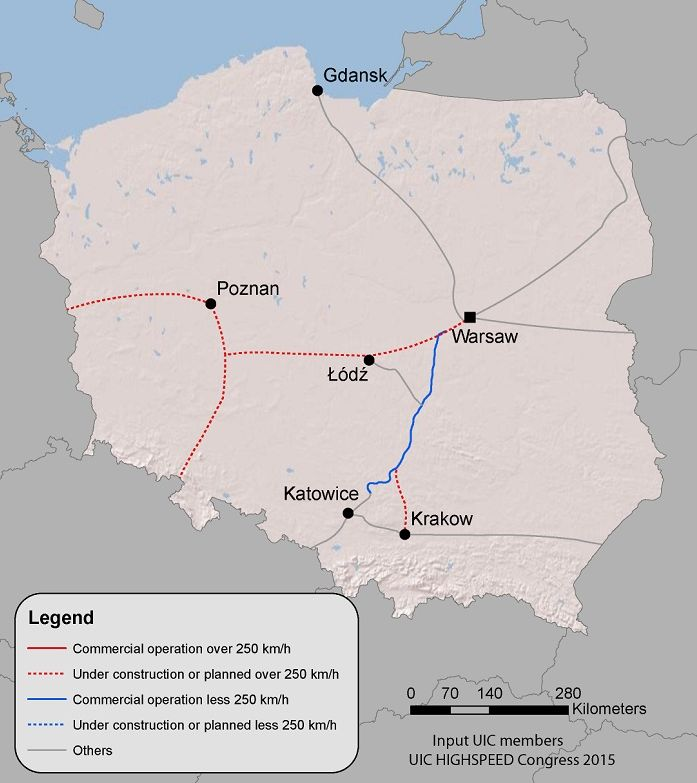
\includegraphics[width=0.7\linewidth]{/mosty_wstep/mapa.jpg}
	\captionsetup{justification=centering}
	\caption{Mapa planowanych i zrealizowanych linii kolejowych dużych prędkości w Polsce - UIC HIGH-SPEED Congress 2015 \parencite{UIC2015}}
	\label{fig:LDP_mapa}
\end{figure}

Pomimo upływu lat nie ulega wątpliwości, że sieć KDP jest kluczowym elementem rozwoju Państwa \parencite{Raczynski2010}. Pozwala zwiększyć atrakcyjność kolei względem pozostałych środków komunikacyjnych, zwiększają spójność państw wchodzących w sieć połączeń, atrakcyjność gospodarczo-społeczną. W 2017 roku przyjęto kolejną uchwałę mówiącej o rozbudowie Kolei Dużych Prędkości w związku z budową Centralnego Portu Komunikacyjnego \parencite{UchwaaNr173}. 


Oczywiście budowa infrastruktury kolejowej wiąże się przekraczaniem przeszkód i budową obiektów inżynierskich. W przypadku KDP jadący tabor musi mieć zagwarantowane restrykcyjne warunki dotyczące bezpieczeństwa przejazdu i komfortu pasażerów. W konsekwencji, przy projektowaniu mostów związane jest to z większym ograniczeniem przemieszczeń i przyspieszeń konstrukcji \parencite{Niemierko}. Dodatkowo wciąż postępujący rozwój technologi, materiałów budowlanych i informatyzacja procesu projektowania sprawiają, że używane są coraz wytrzymalsze materiały w zoptymalizowanych strukturach. Rośnie także zapotrzebowanie na coraz większe, spektakularne konstrukcje pozwalające na przekroczenie dotychczas niepokonanych przeszkód. Sytuacja ta jest szczególnie widoczna w mostach łukowych, popularnych w ciągu tras kolejowych. Pozwalają one na pokonanie większych rozpiętości niż mosty belkowe, a jednocześnie są konkurencyjne cenowo dla mostów kratownicowych (wer.). Nie bez znaczenia, są również aspekty estetyczne. Odczucia obserwatora mostów odnoszą się zarówno do krajobrazowego znaczenia mostu, jak i do aspektu kulturowego i filozoficznego, które w przypadku mostów łukowych są niezwykle silne \parencite{Kido_Cywiński_2019,Kido_Cywiński_2021}. Mosty łukowe z jednej strony naturalnie odnoszone są do pozytywnie odbieranej tęczy \parencite{Prandowski1994}, a z drugiej w miastach mogą stanowić swoistą bramę wjazdową będąc obiektem typu "landmark". W wyniku tych wszystkich czynników budowane konstrukcje są lżejsze i smuklejsze bądź posiadają nietypowe formy. Z reguły wpływa to na zwiększenie podatności na drgania.

\begin{figure}[hbt!]
	\centering
	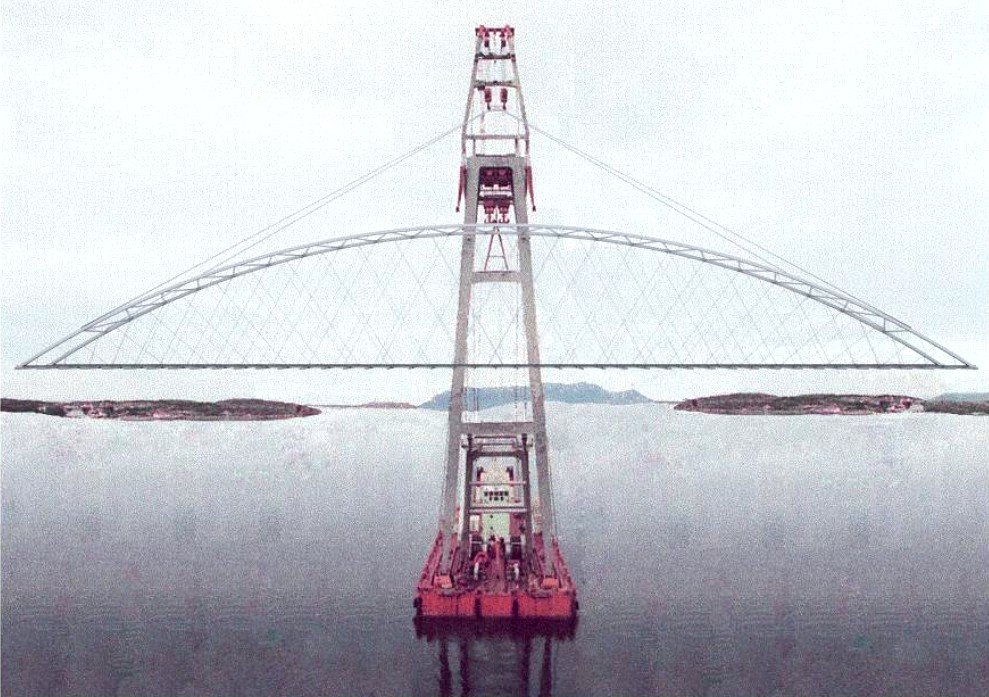
\includegraphics[width=0.7\linewidth]{/mosty_wstep/montaz_akvik_sound_bridge.jpg}
	\captionsetup{justification=centering}
	\caption{Montaż szkieletu mostu drogowego o dźwigarze łukowym i wieszakach typu Network}
	\label{fig:bridges_arch_monatage}
\end{figure}

W tradycyjnym podejściu do projektowania mostów kolejowych największy nacisk stawiano na kwestię wytrzymałości ustroju wyrażoną stanem granicznym nośności z uwzględnieniem trwałości zmęczeniowej. Warunki użytkowe - stan graniczny użytkowania - ograniczały się do sprawdzenia największego ugięcia dźwigarów pod obciążeniem normowym \parencite{PKNf}. W stalowych mostach kolejowych zalecano również sprawdzenie okresu poprzecznych drgań własnych przęsła oraz kątów obrotów na podporach. Uwzględnienie naturalnie dynamicznego zjawiska przejazdu taboru po obiekcie ograniczone było jedynie do zastosowania współczynnika dynamicznego, zwiększającego efekty obciążeń statycznych i nieuwzględniającego efektów rezonansu. Należy stwierdzić, że narzucone normami warunki projektowania sprawdziły się w przypadku mostów kolejowych dla kolei poruszającej się z prędkościami poniżej 160 km/h. W nowszych normatywach jakimi sa Eurokody wyraźnie rozdzielono stan graniczny nośności od stanu granicznego zmęczenia, a także istotnie rozbudowano sprawdzenia stanu granicznego użytkowania oraz weryfikację pracy dynamicznej przęsła. Działania te podjęto na podstawie wniosków i doświadczeń z pracy komitetów naukowych badających efekty przejazdów taboru po mostach. W dużej mierze prace te skupione były na przejazdach z prędkością nawet do 350 km/h. Zidentyfikowano i opisano oddziaływania pionowe i poprzeczne występujące wskutek przejazdu. Obecnie w projektowaniu wymagane jest więc nie tylko by konstrukcja była nośna, ale również należy zagwarantować bezpieczeństwo i komfort użytkowania pasażerów. Narzuca to na barki projektanta szereg nowych obowiązkowych sprawdzeń projektowanej konstrukcji. Dynamika typowych konstrukcji belkowych i płytowych przy przejeździe z dużą prędkością została bardzo dobrze rozpoznana i opisana za pomocą tablic i nomogramów. W pozostałych przypadkach wymagane są zaawansowane i czasochłonne testy numeryczne. 

Mostowe konstrukcje łukowe są bardzo różnorodne. Różnią się położeniem pomostu względem dźwigarów, dystrybucją materiału i sztywności między elementami konstrukcyjnymi czy układem elementów łączących dźwigar łukowy z pomostem. Bogactwo form sprawia, że trudno przewidzieć jaki zestaw parametrów będzie optymalny dla danego usytuowania przeprawy i warunków przejazdu. Wszak w poszukiwaniu najlepszego rozwiązania należy uwzględnić nośność konstrukcji, trwałość, bezpieczeństwo, a aktualnie także również komfort dynamiczny przy przejeździe z dużą prędkością. Przy spełnieniu wszystkich obostrzeń rozwiązanie powinno być również możliwie tanie, aby jej wykonanie było opłacalne i miało szansę powstać. Aktualnie mnogość możliwości ukształtowania konstrukcji, sprawia że ostateczne rozwiązanie jest dalekie od optymalnego technicznie jak i finansowo, co może skutkować jego wykluczeniem z realizacji.


\section*{Cel pracy}
Celem pracy jest określenie wpływu poszczególnych elementów konstrukcyjnych i wyznaczenie ich optymalnych parametrów dla stalowego, kolejowego mostu łukowego z jazdą dołem uwzględniając zachowanie dynamiczne obiektu przy przejeździe pociągów dużej prędkości.
W szczególności wykonane na drodze do głównego rezultatu działania miały na celu:
\begin{enumerate}
	\item zweryfikowanie skuteczności metod operacyjnej analizy modalnej przy identyfikacji modalnej stalowych, kolejowych obiektów łukowych średniej rozpiętości,
	\item opracowanie metodyki kalibracji modelu numerycznego mostu kolejowego za pomocą metod wielokryterialnej optymalizacji globalnej, z wykorzystaniem rezultatów identyfikacji modalnej i standardowych pomiarów prowadzonych w trakcie próbnych obciążeń mostów,
	\item opracowanie metodyki optymalizacji wielokryterialnej mostów kolejowych w ciągu LDP ze szczególnym uwzględnieniem dynamiki konstrukcji,
	\item ocena wpływu poszczególnych parametrów konstrukcji mostu łukowego na zachowanie dynamiczne pod obciążeniem pociągami dużej prędkości.
\end{enumerate}


\section*{Teza pracy}
Możliwe jest znalezienie optymalnego finansowo i dynamicznie rozwiązania konstrukcji mostu łukowego w ciągu linii kolejowych dużych prędkości. Rezultaty optymalizacji mogą pozwolić określić zalecenia doboru parametrów konstrukcji łukowej zapewniające minimalny koszt oraz dostateczną odporność dynamiczną na liniach dużych prędkości.

\section*{Struktura pracy}
Praca składa się z wprowadzenia, pięciu rozdziałów, podsumowania oraz zestawienia bibliograficznego. 

W \textit{Rozdziale 1} przedstawiono wszystkie główne aspekty dotyczące charakterystyki i modelowania mostów łukowych oraz występujących na nich obciążeń dynamicznych. Przedstawiono charakterystykę i klasyfikację mostów łukowych ze szczególnym uwzględnieniem różnic w elementach konstrukcyjnych. W skróconej formie przedstawiono Metodę Elementów Skończonych oraz sposoby kalibracji modelu numerycznego. Na koniec omówiono oddziaływania dynamiczne występujące na mostach kolejowych oraz obowiązujące normatywy w zakresie projektowania tychże mostów. Do każdej z części zaprezentowano obszerny przegląd literatury przedmiotu.

\textit{Rozdział 2} zawiera zbiór podstawowych informacji na temat dynamicznej analizy konstrukcji. W klasyczny sposób rozpoczęto od omówienia ruchu drgającego najprostszego układu - jednego stopnia swobody. Przedstawiono również wielokrotnie użytą w pracy metodę wyznaczania częstotliwości i postaci drgań własnych. Przedstawiono w uporządkowany sposób metody wyznaczania odpowiedzi układu drgającego, zarówno o jednym jak i wielu stopniach swobody. Opisano także miary i modele opisujące efekty tłumienia drgań konstrukcji. Zwrócono uwagę na elementy istotne z punktu widzenia dalszych prac: identyfikacji modalnej konstrukcji i analizy dynamicznej.

Rozdział 3 stanowi opis jednej z rodzin metod identyfikacji modalnej - Operacyjnej Analizy Modalnej. Początkowo przedstawiono koncepcję oraz przytoczono podział i klasyfikację istniejących algorytmów OMA. Zawarto również przegląd literatury mówiącej o zastosowaniach OMA w praktyce inżynierskiej. Do identyfikacji wybranego obiektu badawczego wykorzystano metodę NExT-ERA. Dokonano jej obszernego opisu syntetycznego oraz omówiono właściwości metody. Następnie przedstawiono opis stworzonej aplikacji komputerowej do identyfikacji modalnej bazującej na algorytmie NExT-ERA. Zaprezentowano metody obróbki i łączenia sygnałów, dobór parametrów metody i sposoby oceny poprawności rozwiązania. Wykonano test numeryczny oraz laboratoryjny samej metody jak i stworzonej aplikacji komputerowej.

Rozdział 4 zawiera przedstawienie zagadnienia optymalizacji. Wstępnie omówiono i sklasyfikowano metody optymalizacji w kontekście projektowania konstrukcji. Do dalszych analiz wybrano metodę poszukiwania minimum globalnego algorytmem metaheurystycznym Particle Swarm Optimization (PSO). Opisano metodę oraz dobrane parametry sterujące algorytmem: wielkość roju, warunki brzegowe i topologię roju. Przedstawiono zastosowania algorytmu przy rozwiązywaniu problemów inżynierskich występujące w literaturze. Wykonano przykład teoretyczny metody z jedną funkcją celu. Następnie opisano uogólnienie metody jednokryterialnej do wielokryterialnej z zastosowaniem operatora dominacji w sensie Pareto. Dla wariantu o kilku funkcjach celu również wykonano przykład testowy.

Rozdział 5 jest syntezą wszystkich wcześniej wykonanych prac. Zaprezentowano w nim kompleksową analizę mającą na celu optymalizację konstrukcji istniejącego wiaduktu WK-2 w ciągu Pomorskiej Kolei Metropolitalnej w Gdańsku. Analiza składała się z trzech głównych etapów. Pierwszym była identyfikacja modalna konstrukcji metodą OMA w celu określenia rzeczywistych parametrów modalnych. Następnie przedstawiono procedurę kalibracji modelu numerycznego z zastosowaniem wyników identyfikacji modalnej i badań pod próbnym obciążeniem. Kolejno opisano przeprowadzoną na przygotowanym modelu numerycznym wariantową optymalizację wielokryterialną algorytmem PSO. Przedstawiono rezultaty i wyciągnięto wnioski.

Na końcu rozprawy znajduje się Podsumowanie. Ujęto w nim główne wnioski wynikające z przeprowadzonych prac oraz określono kierunki dalszej pracy nad wykorzystaniem zagadnienia optymalizacji w analizie konstrukcji mostowych.







%Kolejowe mosty łukowe
\chapter{Kolejowe mosty łukowe poddane obciążeniom dynamicznym}
\textit{Streszczenie: W niniejszym rozdziale dokonano ogólnej charakterystyki mostów łukowych oraz problematyki obciążeń dynamicznych. Opis poparto obszernym studium prac traktujących o tych zagadnieniach. Na początku sklasyfikowano obiekty łukowe oraz przedstawiono kluczowe z punkty widzenia dalszych prac elementy konstrukcyjne. Następnie, krótko opisano ideę metody elementów skończonych oraz metody \higg{kalibracji} modeli numerycznych. W dalszej części rozdziału omówiono aktualny stan wiedzy i zapisy prawne dotyczące dynamicznych obciążeń kolejowych. Opisano jakie obciążenia dynamiczne występują na mostach kolejowych oraz zaprezentowano metody ich uwzględniania, zwracając uwagę szczególnie na koleje dużych prędkości.}

\vspace{1cm}

W celu łatwiejszego odbioru dalszych rozważań, na wstępie przedstawiono klasyfikację mostów łukowych. Konstrukcje mostów, których elementem jest dźwigar nośny w postaci łuku mają długą historię. Ewolucja techniki sprawiła, że na przestrzeni lat zrealizowano szeroką gamę obiektów z odmiennych materiałów i o różnych schematach statycznych. Usystematyzowanie tej wiedzy jest kluczowe w podjęciu dalszych rozważań nad dopuszczalnymi rozwiązaniami w procesie optymalizacji. Podobnie należy potraktować oddziaływania dynamiczne na mostach kolejowych. Ich szczegółowe rozpoznanie - przedstawione w poniższym rozdziale - pozwala uwzględnić w analizach tylko te efekty, które są istotne z punktu widzenia dynamiki konstrukcji mostowej.

\section{Układ statyczny i elementy konstrukcyjne mostów łukowych}

Tradycyjnie mosty łukowe wykonywane były jako pełne sklepienia, ze ściankami czołowymi i z wnęką wypełnioną piaskiem, żwirem lub słabym betonem. Ukształtowany w ten sposób ustrój mógł być wykonany z najstarszych surowców, takich jak kamień \parencite{Szczygie1978}. Obecnie tego typu obiekty wykonuje się niezmiernie rzadko. Służyły one do przekraczania małych i średnich rozpiętości (do ok. 40 m) i w dzisiejszych czasach zostały wyparte głównie przez strunobetonowe konstrukcje prefabrykowane \parencite{Ciesla2013} i obiekty gruntowo-powłokowe \parencite{Janusz2009,Tomala2019}. Podobną formę geometryczną, ze ścianami czołowymi działającymi jako elementy konstrukcyjne stanowią łuki tarczowe. Dzięki uwzględnieniu pracy tarczowej ścianek czołowych są one efektywniejsze niż bliźniacze łuki sklepione. Jednakże obecnie mosty łukowe wykonuje się głównie w formie konstrukcji belkowo-płytowych. 


\subsubsection{Schemat statyczny i kształt konstrukcji}
Z punktu widzenia schematu statycznego dźwigara łukowego wyróżnia się łuki bezprzegubowe (utwierdzone), dwuprzegubowe i trójprzegubowe. Wybór schematu statycznego miał niegdyś większe znaczenie ze względu na różny stopień złożoności obliczeniowej. Obecnie analiza układów statycznie niewyznaczalnych nie stanowi problemu dzięki wykorzystaniu metod komputerowych (np. MES). Brak potrzeby dążenia do statycznej wyznaczalności, bez popełnienia błędu obliczeniowego pozwala wyeliminować z wnętrza konstrukcji przeguby. Są one z punktu widzenia trwałości konstrukcji elementami niepożądanymi. Z drugiej strony, układy statycznie wyznaczalne są odporne na obciążenia drugorzędne i należy je stosować w przypadku zagrożenia na przykład przemieszczeniem podpór. Niezależnie od zmian w podejściu do projektowania, przy przyjęciu teoretycznego schematu statycznego warto pamiętać, że aktualną pozostaje reguła przywołana przez profesora Andrzeja Pszenickiego \cite{Pszenicki1954}: \textquote{Zasadą jest, że obliczenie powinno odpowiadać konstrukcji (...).}. Stąd wybór schematu statycznego nie może być jedynie odgórnym założeniem przyjętym przez projektanta, ale również musi uwzględniać możliwości ukształtowania warunków brzegowych rzeczywistej konstrukcji. 

Ze względu na wzajemne usytuowanie pomostu i dźwigarów łukowych można wyszczególnić następujące formy konstrukcji mostu:
\begin{itemize}
	\item most z jazdą górą - pomost usytuowany jest w całości nad łukiem - na przykład rys. \ref{fig:bri_deck_loc_top}, \ref{fig:arch_deck_bridges_a},
	\item most z jazdą dołem - pomost usytuowany jest w całości poniżej łuku - na przykład rys. \ref{fig:bri_deck_loc_middle}, \ref{fig:arch_deck_bridges_d},
	\item most z jazdą pośrednią - pomost usytuowany jest pośrednio - na przykład rys. \ref{fig:bri_deck_loc_bott}, \ref{fig:arch_deck_bridges_e}.
\end{itemize}

\begin{figure}[hbt!]
	\centering
	\subfloat[most łukowy z jazdą górą]{\includegraphics[width=0.7\linewidth,page=4]{/mosty_wstep/mosty.pdf} \label{fig:bri_deck_loc_top}}  \\
	\subfloat[most łukowy z jazdą pośrednią]{\includegraphics[width=0.7\linewidth,page=6]{/mosty_wstep/mosty.pdf} \label{fig:bri_deck_loc_middle}} \\
	\subfloat[most łukowy z jazdą dołem]{\includegraphics[width=0.7\linewidth,page=5]{/mosty_wstep/mosty.pdf} \label{fig:bri_deck_loc_bott}}
	\captionsetup{justification=centering}
	\caption{Klasyfikacja mostów łukowych ze względu na wzajemne położenie pomostu i dźwigara}
	\label{fig:bridges_types_deck_location}
\end{figure}

%\begin{figure}[bt!]
%	\centering
%	\captionsetup{justification=centering}
%	
%	\subfloat[Wiadukt WK-11 w ciągu PKM Gdańsk (fot. materiały archiwalne firmy Keller)]{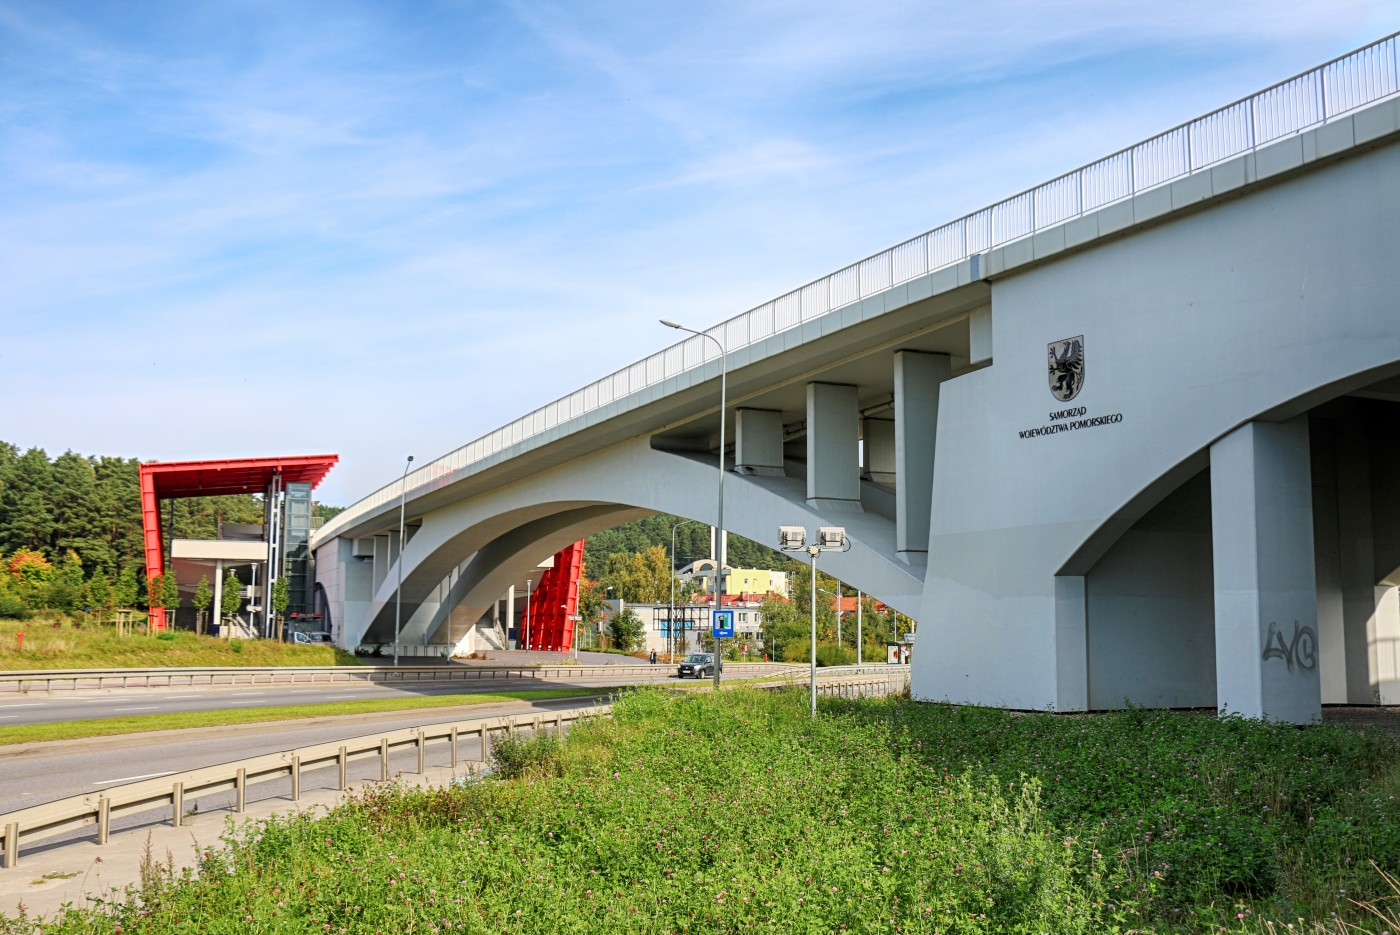
\includegraphics[width=0.48\linewidth]{/mosty_wstep/photos/keller-polska-pale-cfa-pkm-gdansk-8.jpg} \label{fig:arch_deck_bridges_a}} \;
%	%
%	\subfloat[Most im. Marszałka Piłsudzkiego w Krakowie (fot. Jakub Hałun/wikipedia.org)]{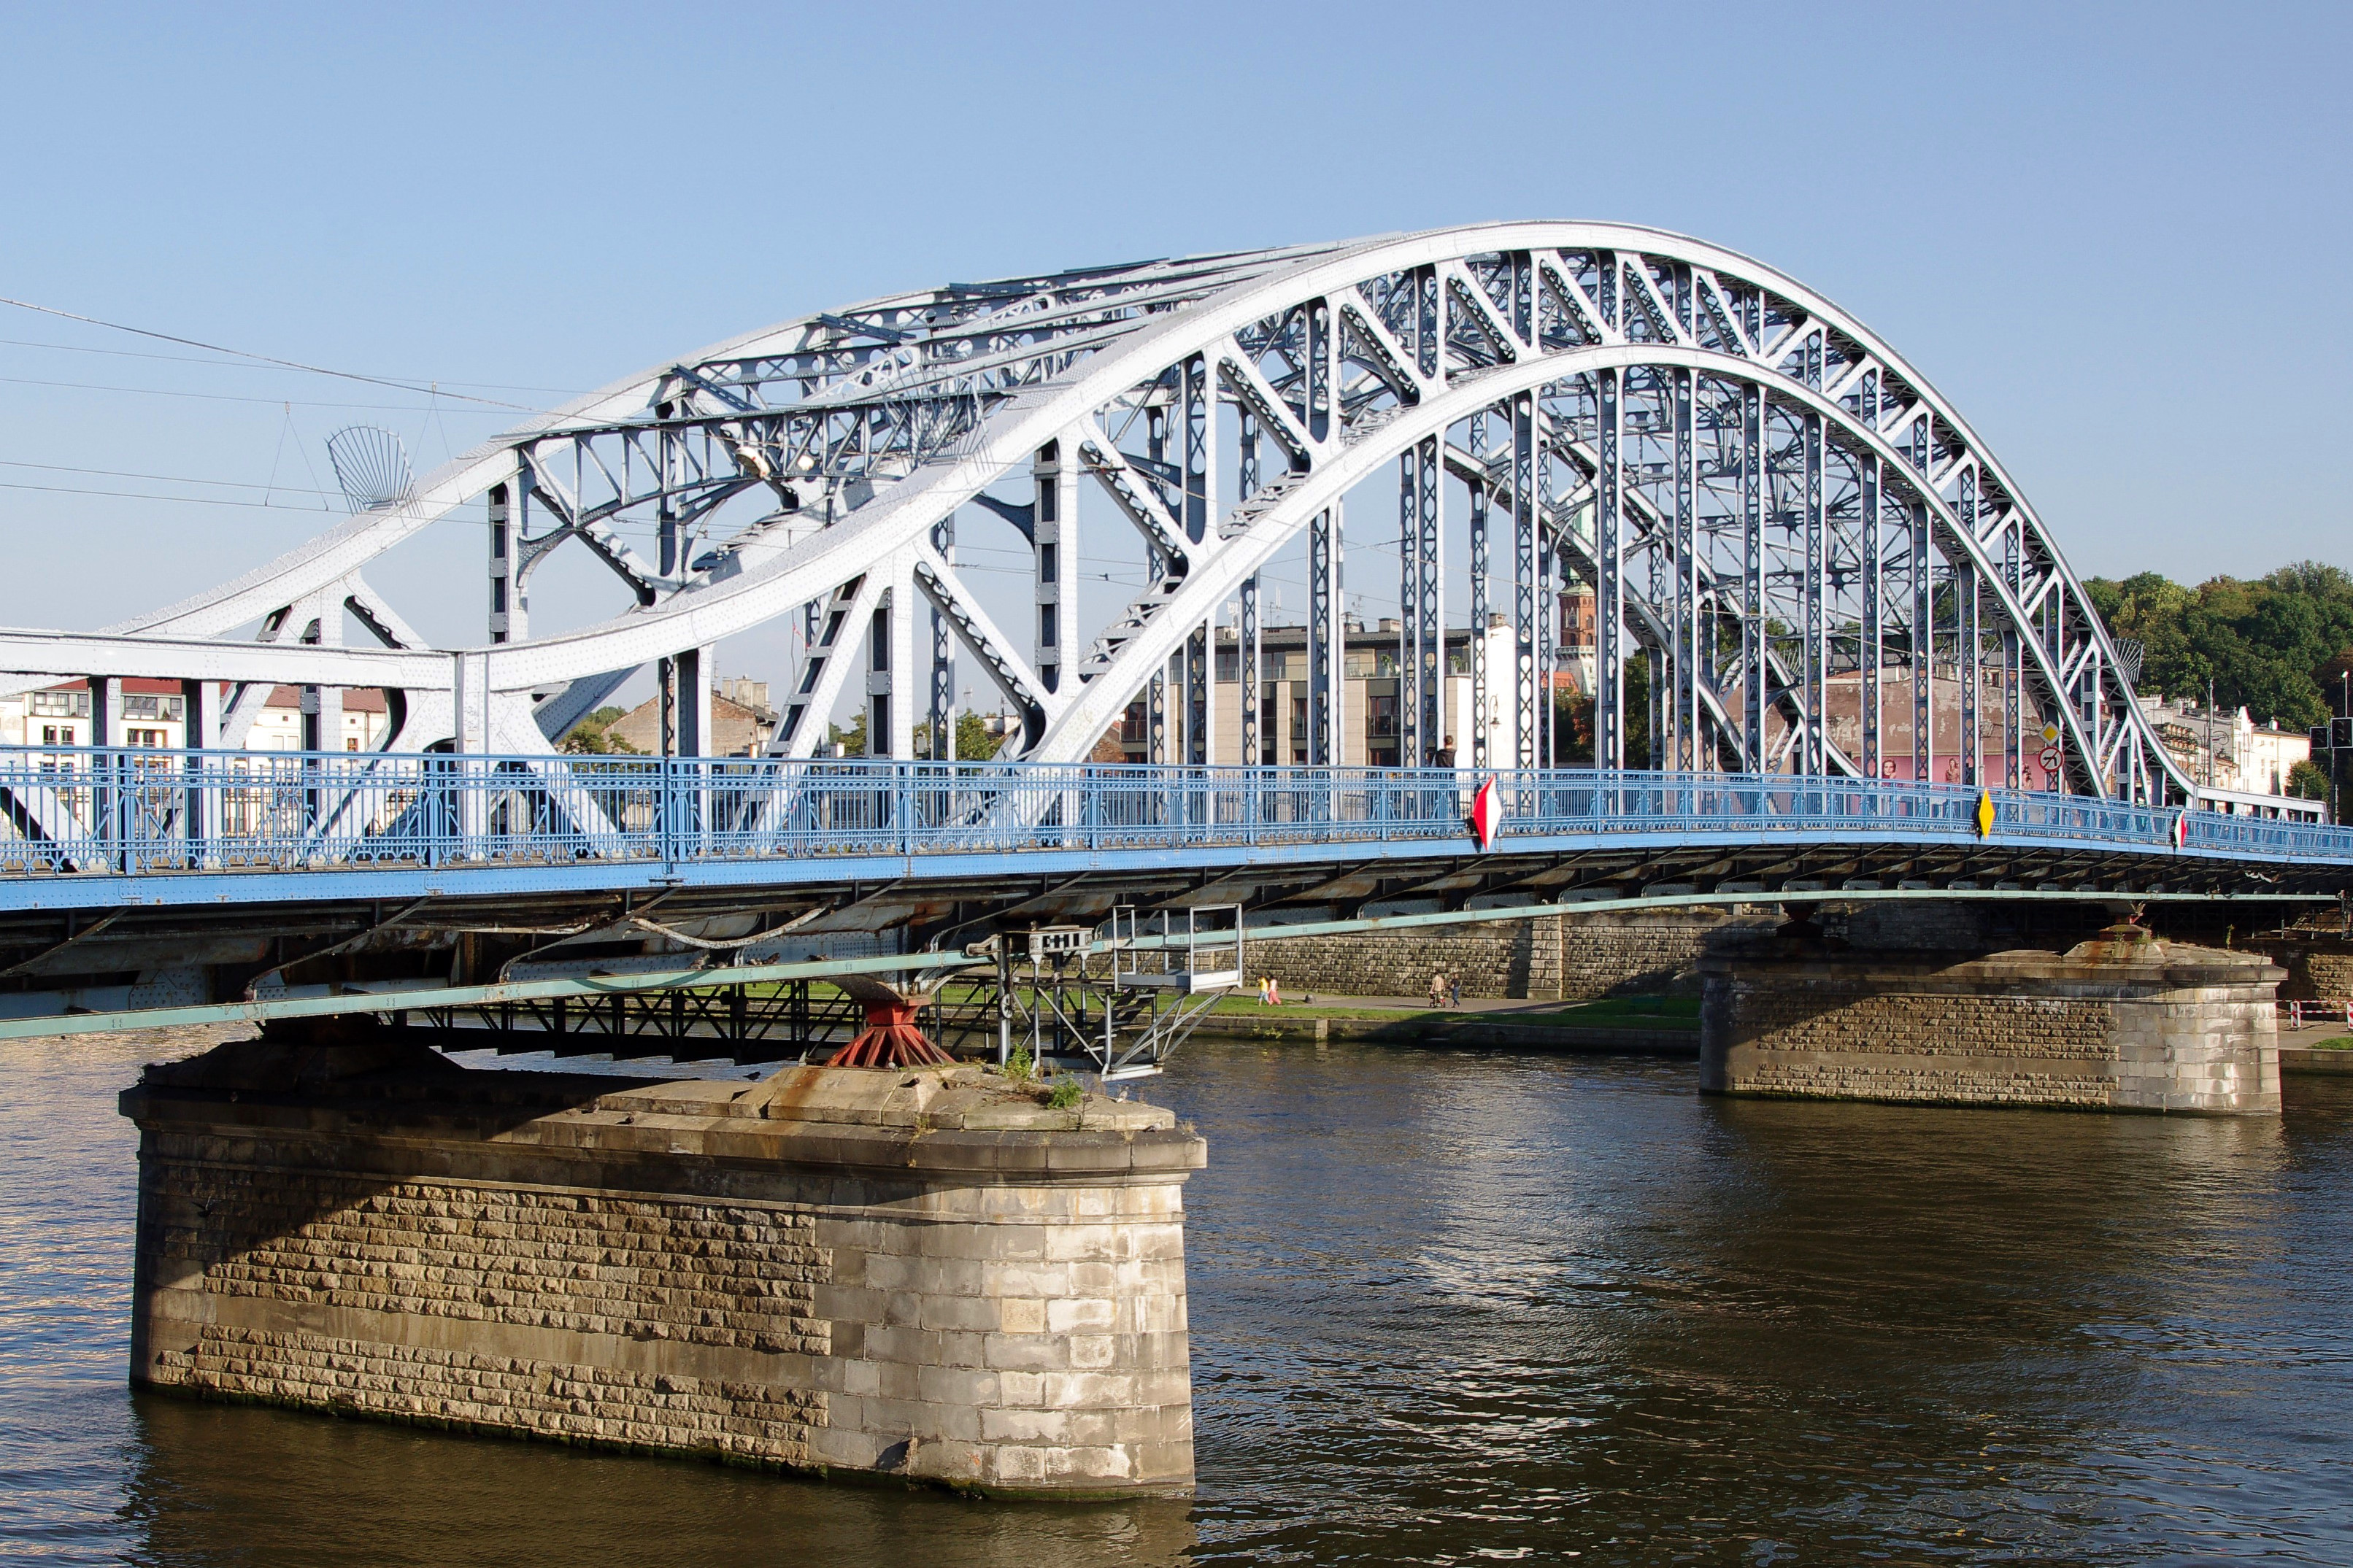
\includegraphics[width=0.48\linewidth]{/mosty_wstep/photos/Krakow_most_Pilsudskiego.jpg} \label{fig:arch_deck_bridges_b}} \\
%	%
%	\subfloat[Most im. Jana Pawła II w Puławach\\(fot. Kamil Lewandowski/Gmina Puławy)]{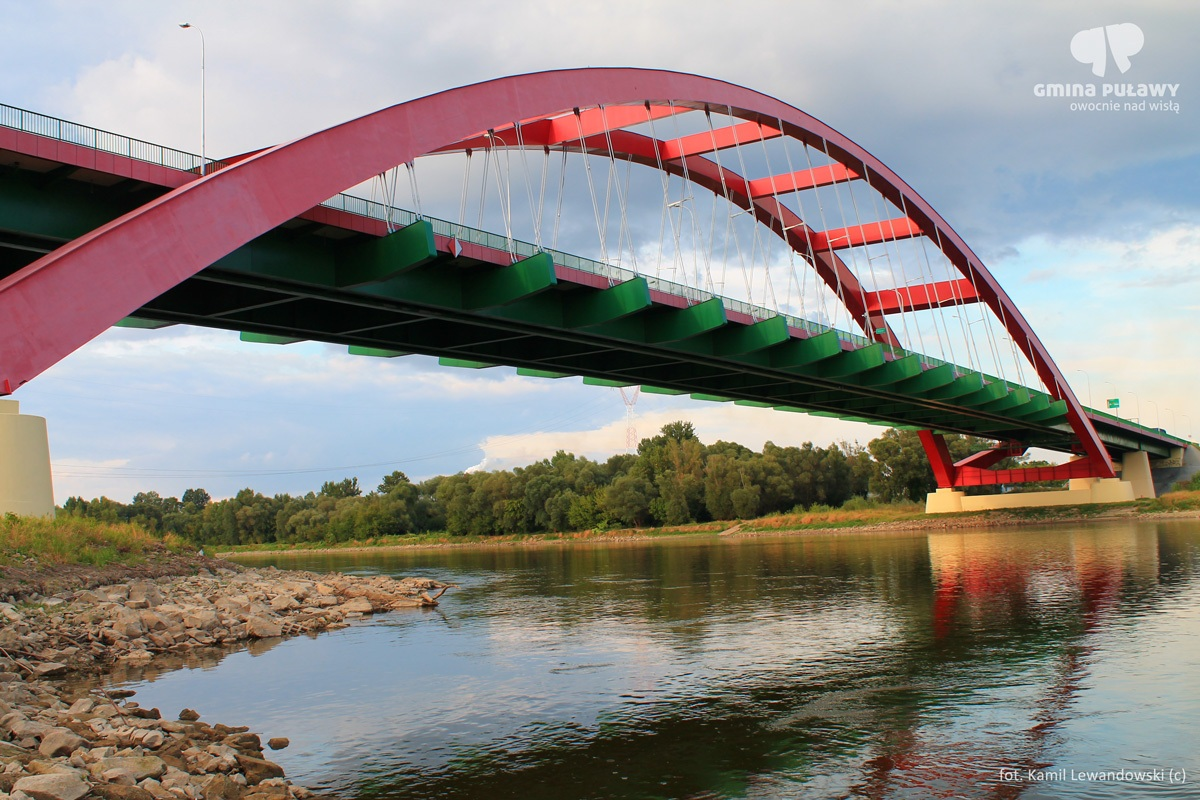
\includegraphics[width=0.48\linewidth]{/mosty_wstep/photos/most_pulawy.jpg} \label{fig:arch_deck_bridges_c}} \;
%	%
%	\subfloat[Most na Dziwnie w ciągu obwodnicy Wolina\\(fot. Radosław Drożdżewski)]{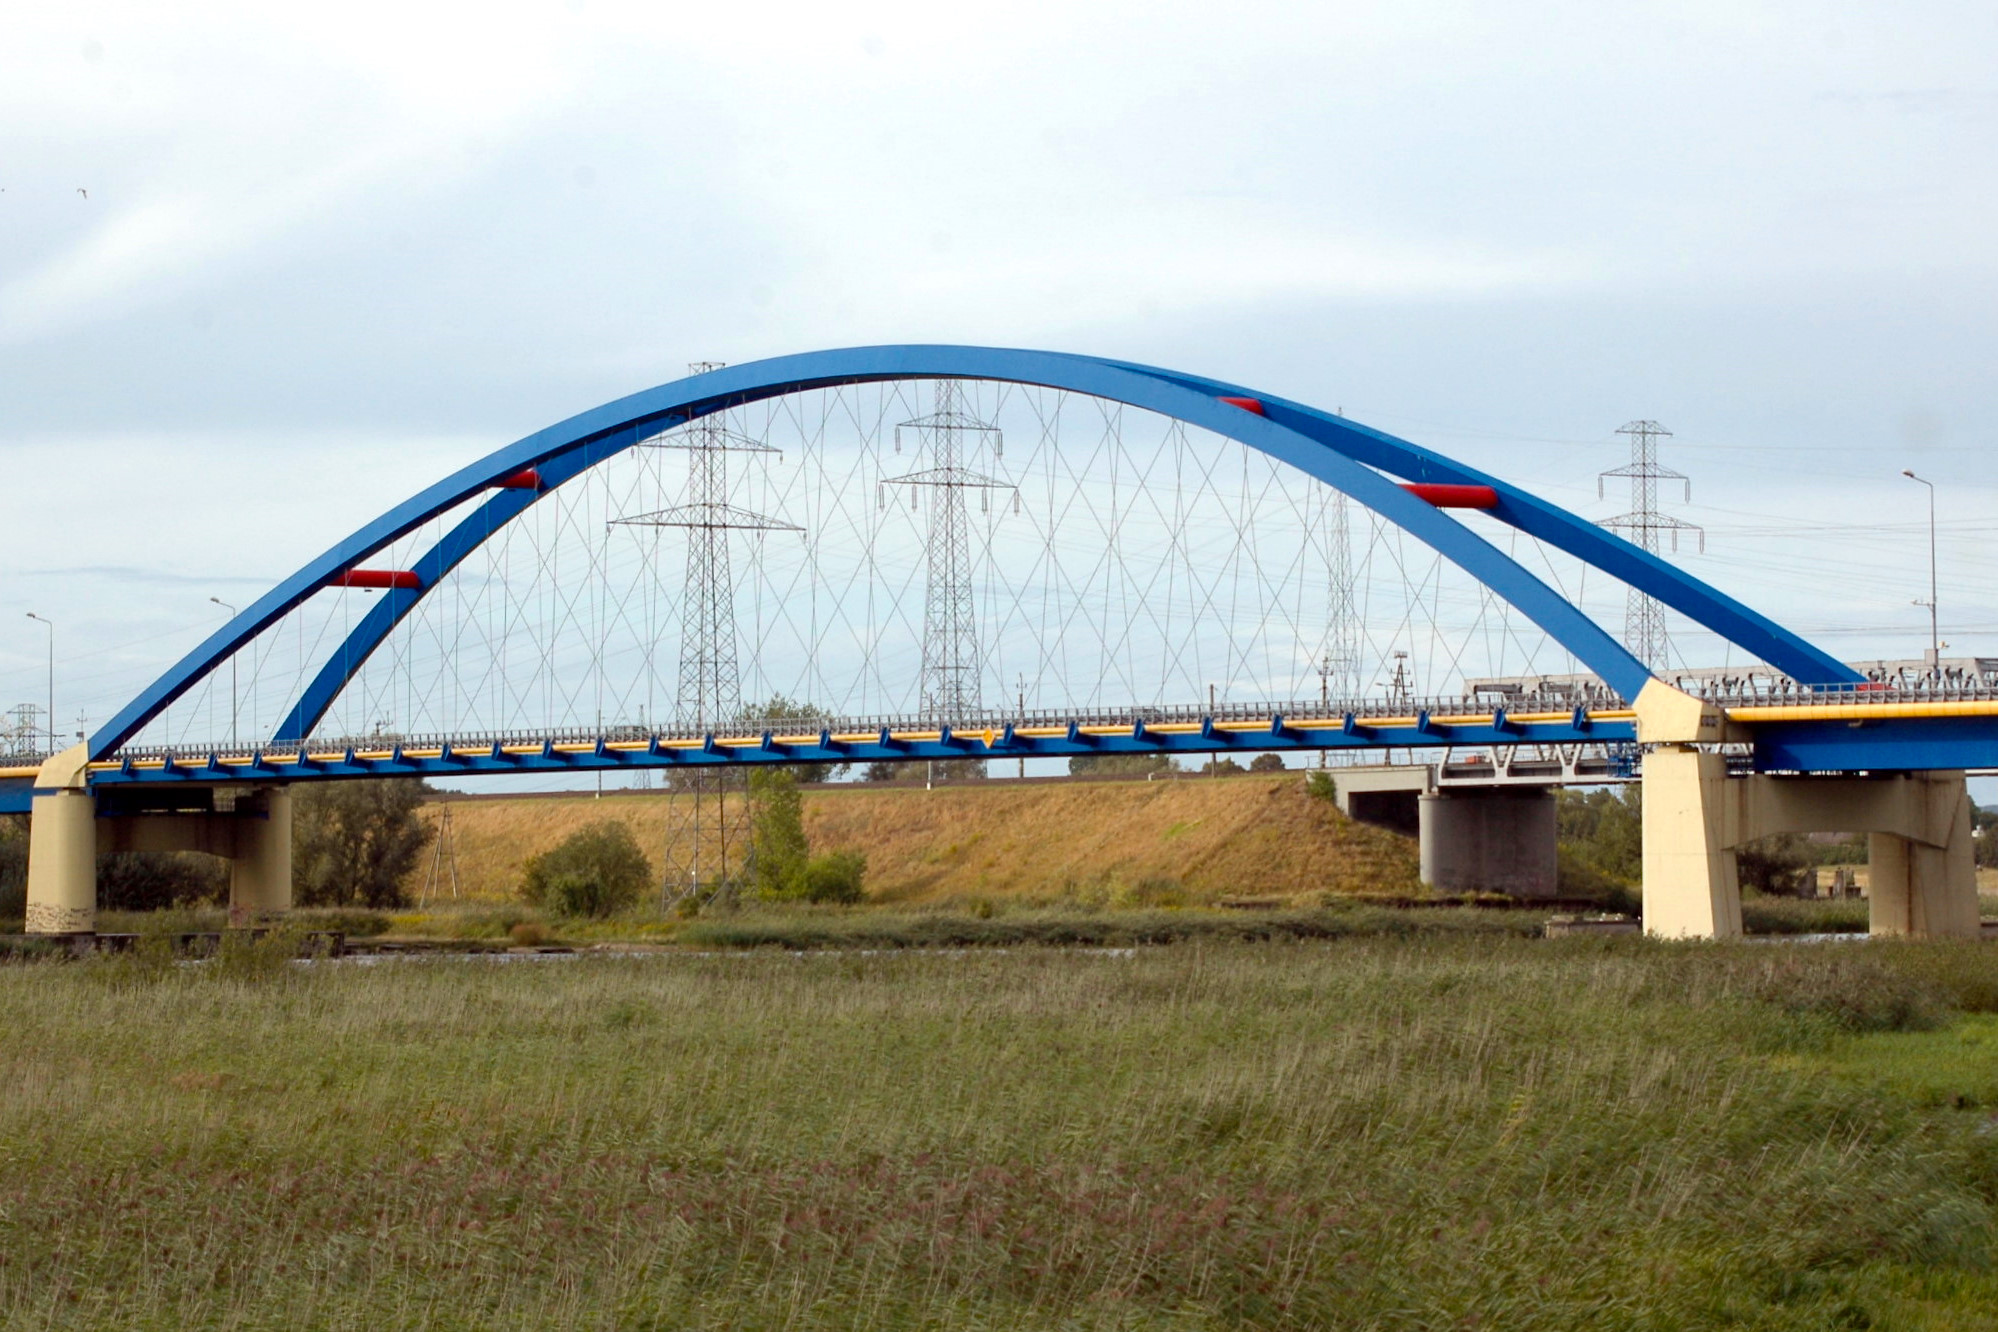
\includegraphics[width=0.48\linewidth]{/mosty_wstep/photos/Wolin_-_most_obwodowy_DK3_d_radoslaw_drozdzewski.jpg} \label{fig:arch_deck_bridges_d}}
%	%
%	\caption{Wybrane polskie mosty łukowe: (a) wiadukt z jazdą górą i dźwigarem żelbetowym, (b) most z jazdą dołem i dźwigarem kratowym, (c) most z jazdą pośrednią i dźwigarem stalowym, (d) most z jazdą dołem i dźwigarem stalowym}
%	\label{fig:arch_deck_bridges}
%\end{figure}

\begin{figure}[p]
	\centering
	\captionsetup{justification=centering}
	
	\subfloat[Wiadukt WK-11 w ciągu PKM Gdańsk (arch. własne)]{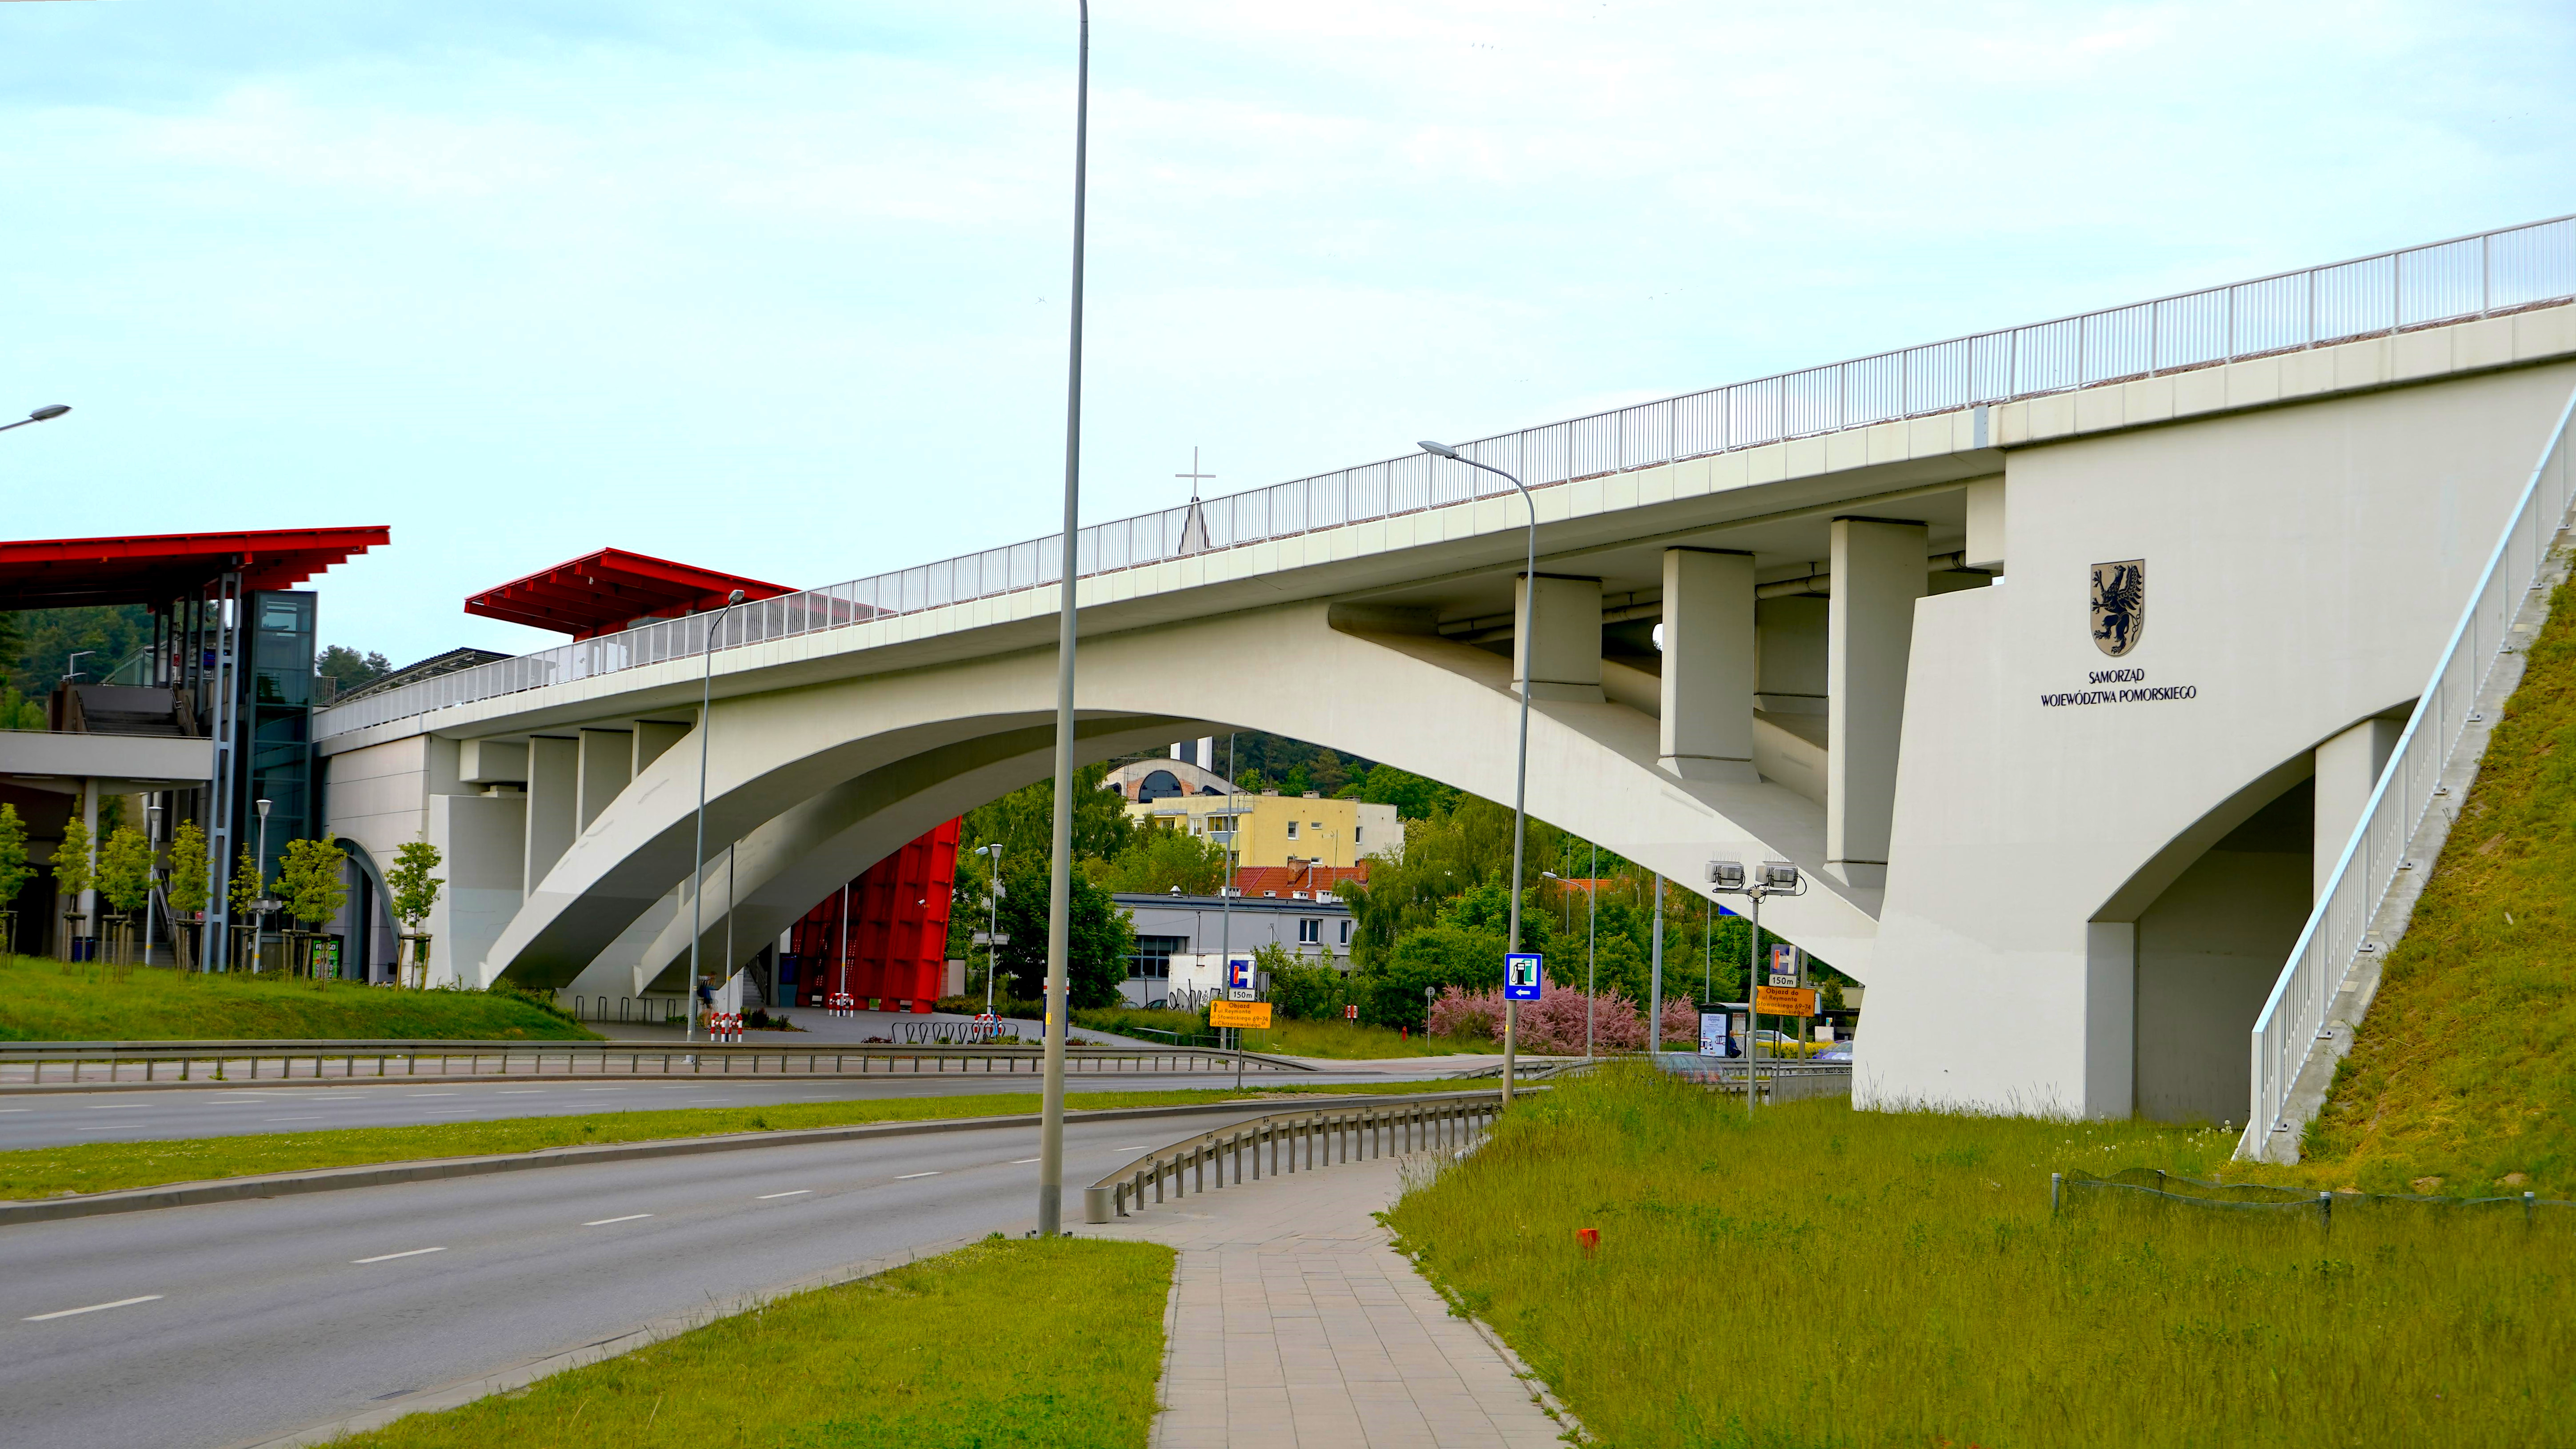
\includegraphics[width=0.48\linewidth]{/mosty_wstep/photos/kolejowy_slowackiego_1.jpg} \label{fig:arch_deck_bridges_a}} \;
	%
	\subfloat[Wiaduk kolejowy nad ul. Hallera w Gdańsku (arch. własne)]{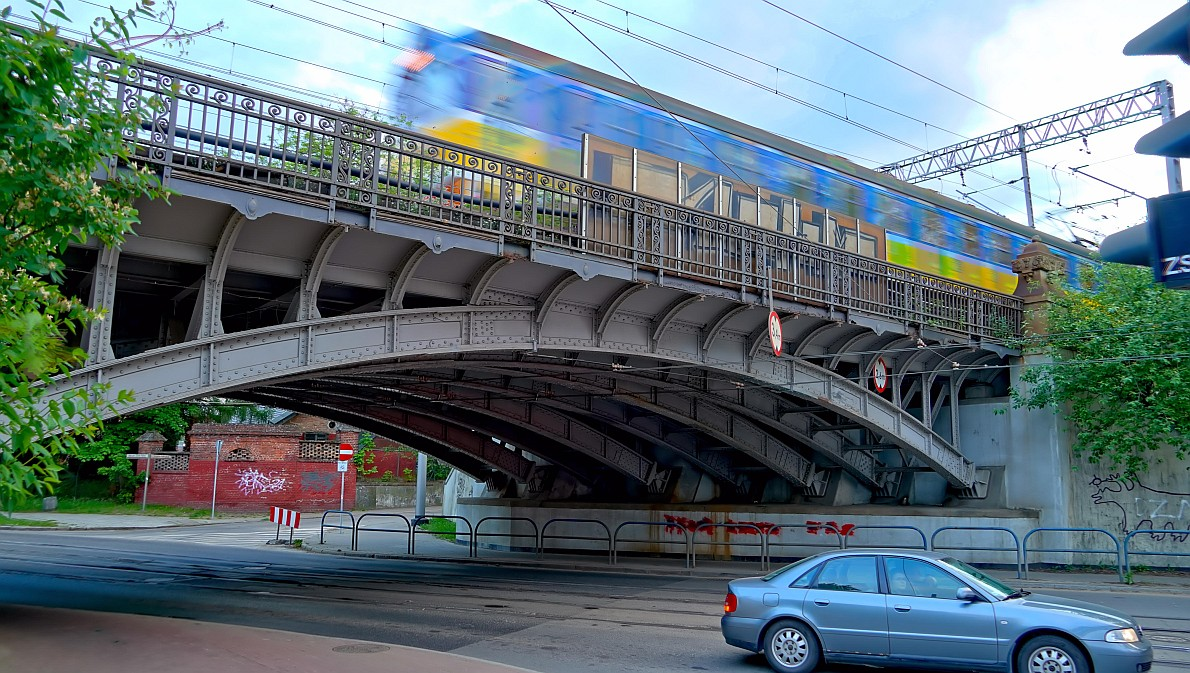
\includegraphics[width=0.48\linewidth]{/mosty_wstep/photos/kolejowy_hallera.jpg} \label{fig:arch_deck_bridges_b}} \\
	%
	\subfloat[Wiaduk drogowy w ciągu al. Żołnierzy Wyklętych w Gdańsku (arch. własne)]{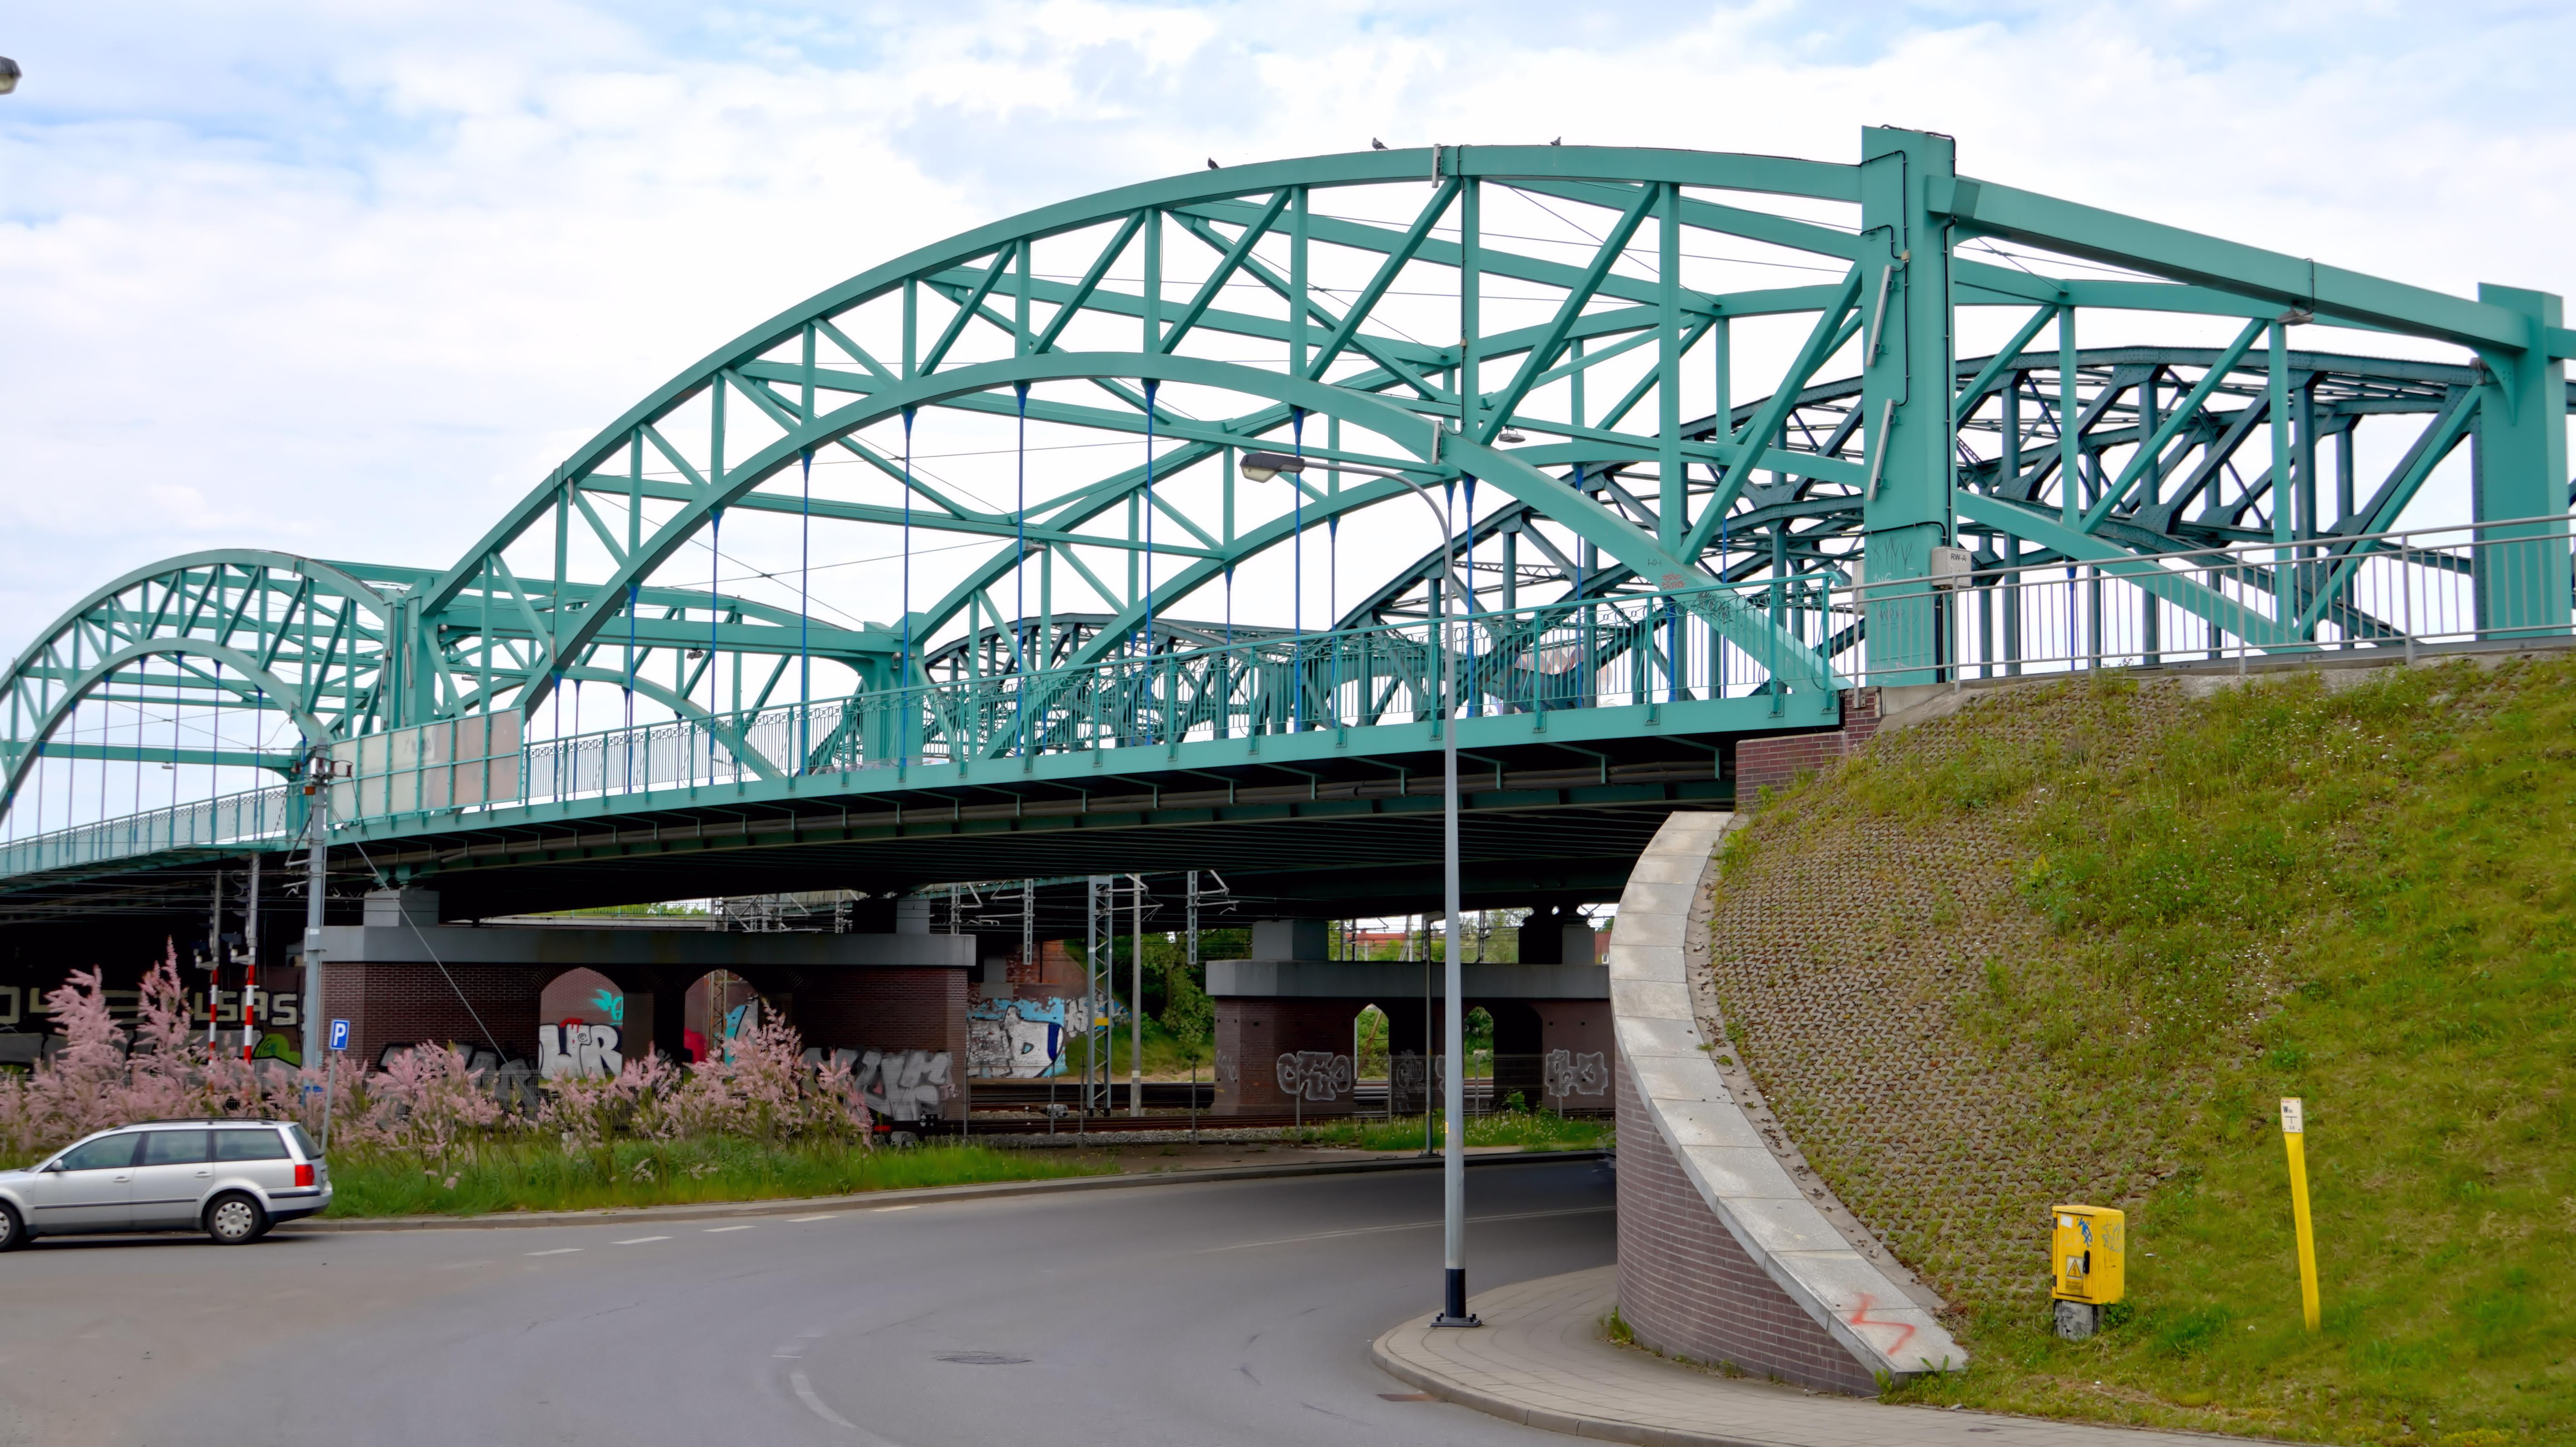
\includegraphics[width=0.48\linewidth]{/mosty_wstep/photos/lukowy_kolo_GB.jpg} \label{fig:arch_deck_bridges_c}} \;
	%
	\subfloat[Most kolejowy przez Martwą Wisłę w Gdańsku (arch. własne)]{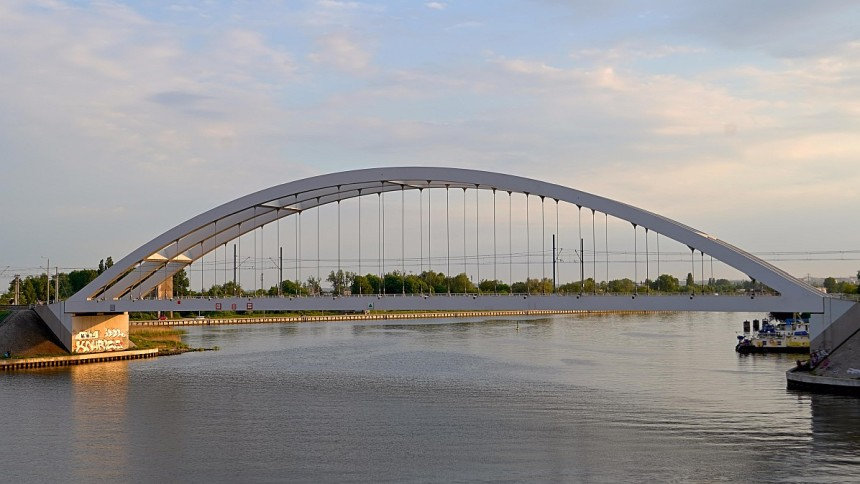
\includegraphics[width=0.48\linewidth]{/mosty_wstep/photos/kolejowy_martwa_wisla.jpg} \label{fig:arch_deck_bridges_d}} \\
	%
	\subfloat[Kładka dla pieszych przez Obwodnicę Trójmiasta (arch. własne)]{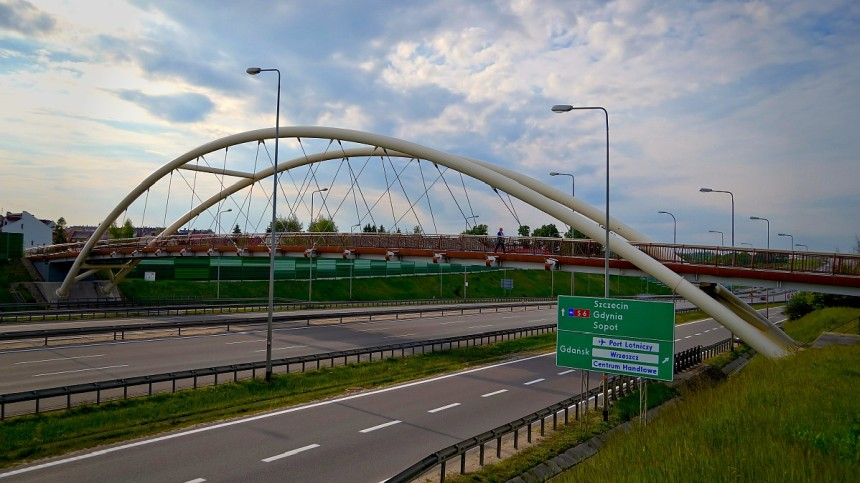
\includegraphics[width=0.48\linewidth]{/mosty_wstep/photos/kladka_obwodnica_1.jpg} \label{fig:arch_deck_bridges_e}} \;
	%
	\subfloat[Wiadukt drogowy w ciągu ul. Armii Krajowej w Bydgoszczy (arch. własne)]{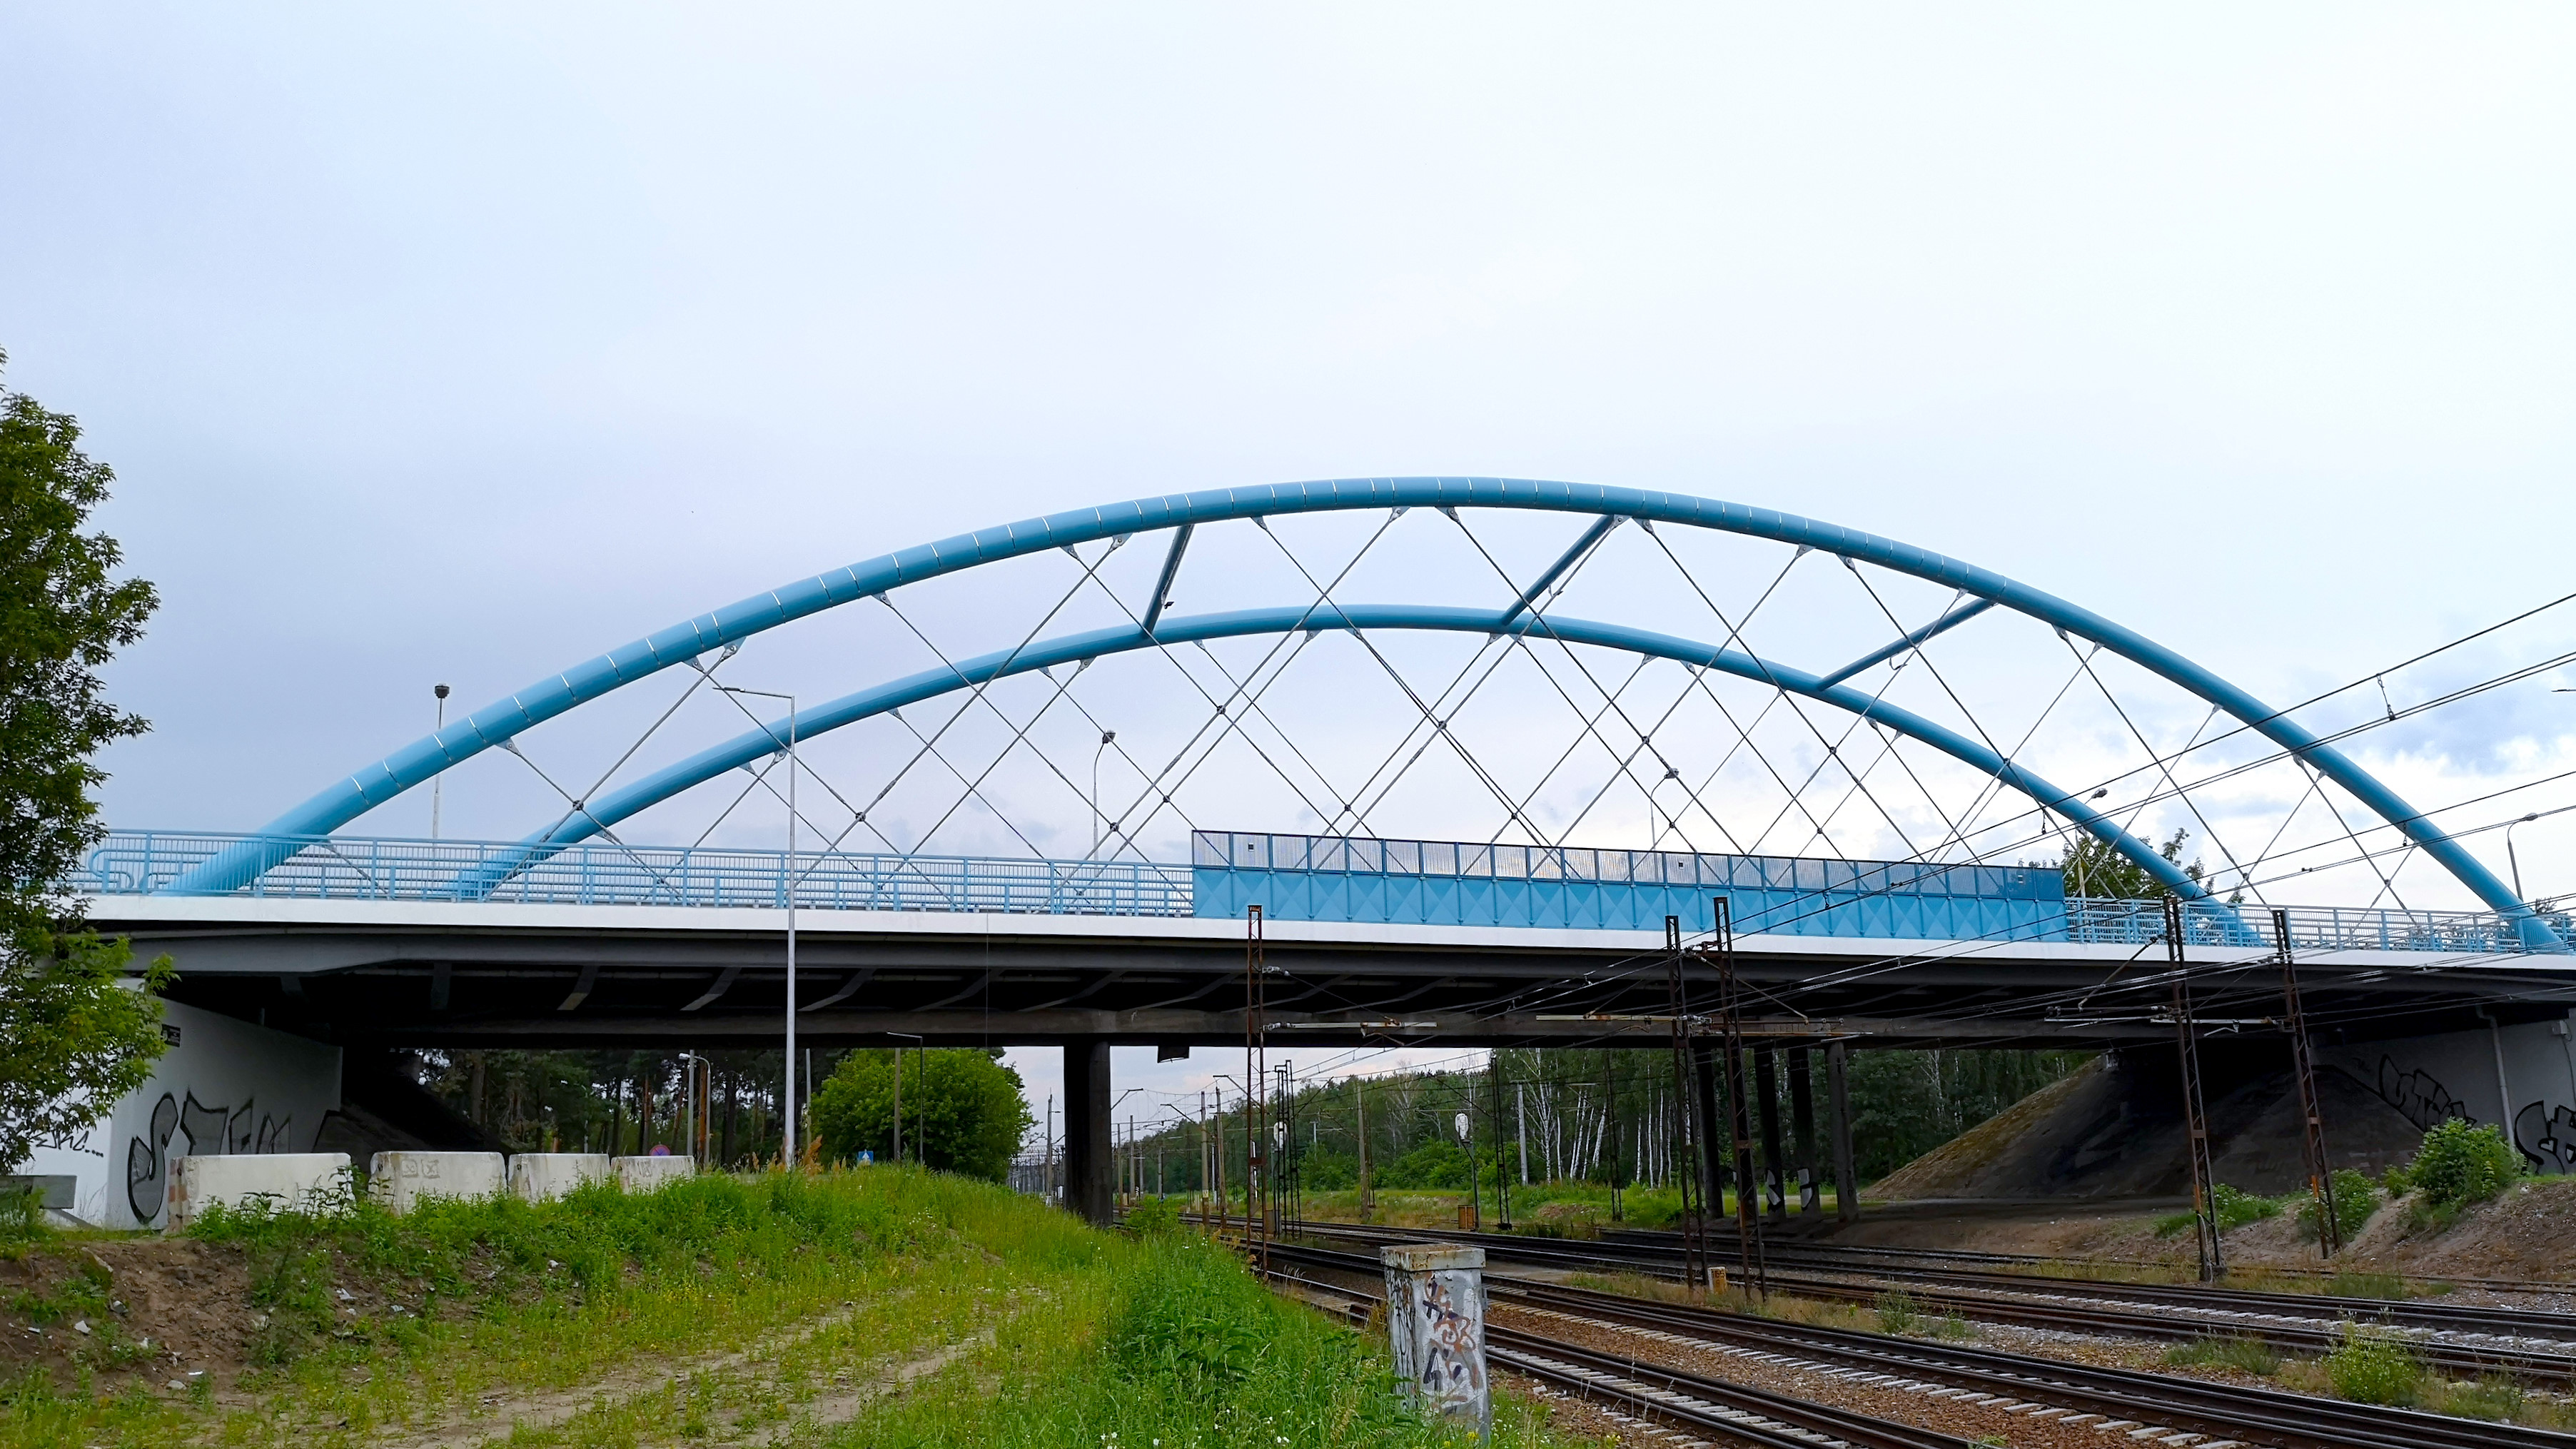
\includegraphics[width=0.48\linewidth]{/mosty_wstep/photos/wiadukt_bydgoszcz.jpg} \label{fig:arch_deck_bridges_f}} \\
	%
	\subfloat[Wiadukt w ciągu Obwodnicy Południowej - węzeł Gdańsk Południe (arch. własne)]{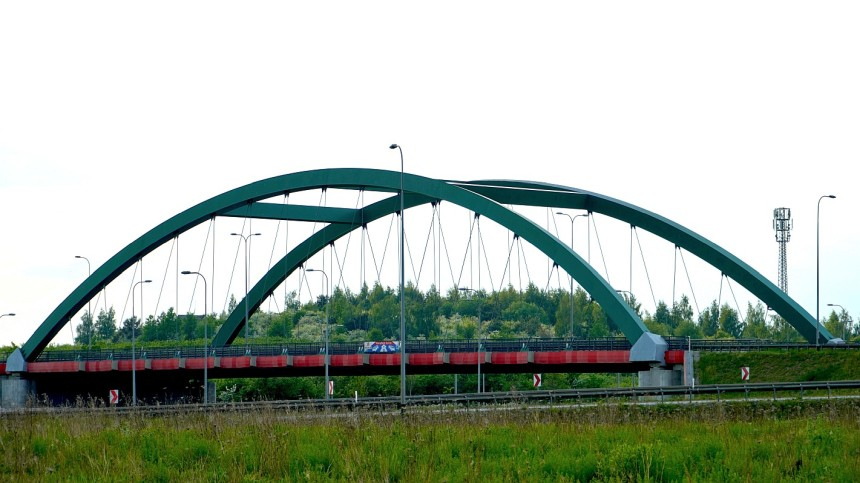
\includegraphics[width=0.48\linewidth]{/mosty_wstep/photos/kolejowy_POG_1_1.jpg} \label{fig:arch_deck_bridges_g}} \;
	%
	\subfloat[Wiadukt WD0 nad Obwodnicą Wałcza w trakcie próbnego obciążenia (arch. własne)]{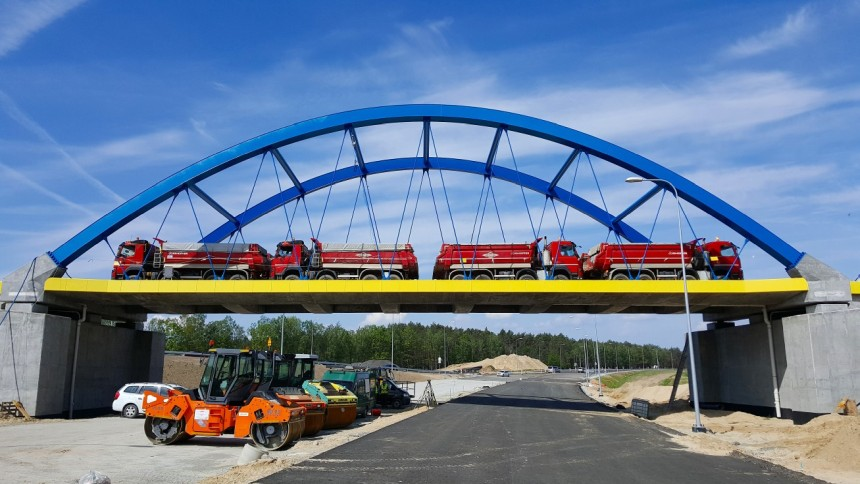
\includegraphics[width=0.48\linewidth]{/mosty_wstep/photos/probne_walcz_1.jpg} \label{fig:arch_deck_bridges_h}}
	%
	\caption{Wybrane polskie mosty łukowe: (a) wiadukt z jazdą górą i dźwigarem żelbetowym, (b) wiadukt z jadą górą i dźwigarem stalowym, (c) wiadukt z jazdą dołem i dźwigarem kratowym, (d) most z jazdą dołem i dźwigarem stalowym, (e) kładka dla pieszych z wieszakami typu Network, (f) wiadukt z wieszkami typu Network, (g) wiadukt z wieszkami Nielsena, (h) wiadukt z wieszkami Nielsena w trakcie próbnego obciążenia}
	\label{fig:arch_deck_bridges}
\end{figure}

Mosty z jazdą górą budowane są kiedy pod obiektem jest na tyle dużo miejsca, że możliwe jest zastosowanie dużej wysokości konstrukcyjnej. Taka sytuacja ma miejsce na przykład w terenach górzystych. W przeciwnym przypadku gdy wymagana jest mała wysokość konstrukcyjna uzasadnione jest stosowanie obiektów z jazdą dołem lub pośrednią. 

Obciążona konstrukcja łukowa z zasady generuje siły poziome na podłoże. Nazywa się je reakcjami rozporowymi lub po prostu rozporem. W przypadku obiektów z jazdą dołem lub jazdą pośrednią możliwe jest wyeliminowanie reakcji poziomych przez zastosowanie ściągu. Rolę ściągu może stanowić odrębny element konstrukcyjny jak również cały pomost. Wykorzystanie pomostu jest obecnie bardzo częstym rozwiązaniem. Dotyczy to zarówno pomostów stalowych jak i betonowych. W przypadku pomostów betonowych stosuje się sprężenie niwelujące efekt rozciągania pochodzącego od rozporu.

Mosty łukowe wykonywane są aktualnie głównie z dwóch materiałów: stali i betonu (w tym betonu sprężonego i kompozytu CFST \teng{Concrete Filled Steel Tubes}). Zależnie od materiału dźwigar łukowy może posiadać różną strukturę. Najczęściej łuki występują w następujących formach \parencite{Cholewo1965}:
\begin{itemize}
	\item pełnościenny stalowy przekrój łuku (Rys. \ref{fig:arch_deck_bridges_b}),
	\item łuk w postaci stalowej kratownicy (Rys. \ref{fig:arch_deck_bridges_c}),
	\item pełny betonowy przekrój lub w postaci skrzynki (Rys. \ref{fig:arch_deck_bridges_a}),
	\item zespolony przekrój ze stalowym płaszczem wypełnionym betonem (CFST) \parencite{Abramski2019}.
\end{itemize}

W przeważającej większości mosty łukowe projektowane są obecnie jako konstrukcje statycznie niewyznaczalne. Z tego względu mogą one różnić się mechanizmem pracy również w zależności od wzajemnej sztywności poszczególnych elementów konstrukcyjnych. \todo{Dodano wariant ze sciagiem}\higr{W klasycznym rozwiązaniu łuk zdecydowanie dominuje sztywnością nad ściągiem i to łuk przenosi zarówno siły osiowe jak i ewentualne momenty zginające. Wówczas rolą ściągu jest przeniesienie przede wszystkim sił rozporu.} Kiedy zarówno łuk jak i dźwigar pomostu odpowiadają za przeniesienie sił normalnych i momentów zginających mamy do czynienia z układem Lohse'a. Przypadek ten wystąpi kiedy łuk i ściąg posiadają znaczącą sztywność giętną. Odmienna sytuacja występuję w przypadku układu Langera, kiedy to wiotki dźwigar łukowy \textit{de facto} jedynie usztywnia dźwigar belkowy. W tej sytuacji łuk przenosi teoretycznie jedynie siły osiowe \parencite{Lin2017}. 

Standardowe rozpiętości dla przęseł łukowych kształtują się w zakresie od 40 do około 400 m w przypadku mostów betonowych i do 500 m w przypadku mostów stalowych \parencite{Madaj2009}. W pracy \cite{Czudek1997} autor przedstawił typowe rozpiętości dla mostów stalowych, w zależności od rodzaju przęsła łukowego. Dla tradycyjnych przęseł łukowych podał zakres od 40 do 300 m, dla łuków typu Langera od 40 do 150 m, dla łuków typu Lohse'a od 60 do 200 m, a dla łuków Nielsena i Network (Rys. \ref{fig:bridges_types_hangers}) od 110 do 200 m. Aktualnie (maj 2021) na światowej liście mostów łukowych o największej rozpiętości pierwsze miejsce zajmuje chiński most \textit{Pingnan Third Bridge} (Rys. \ref{fig:arch_bridges_a} \parencite{Contributors2021,Biliszczuk2015a}. Został on oddany do użytku 28 grudnia 2020 roku, a jego rozpiętość wynosi 575 m. Warto zauważyć, że na liście obiektów o rozpiętości powyżej 300 m znajduje się obecnie 76 pozycji z czego zdecydowaną większość (47 pozycji) stanowią mosty chińskie, a drugą pozycję pod względem liczebności zajmują Stany Zjednoczone Ameryki z 9 obiektami. Pod względem materiałów wykorzystanych do budowy łuku większość przęseł wykonana  jest ze stali (44 pozycje). Pozostałe obiekty zbudowane są z elementów CFST (19 pozycji) i betonu (13 pozycji). Najstarszy na liście obiekt \textit{Bayonne Bridge} został oddany do użytku w 1931 roku i wciąż zajmuje wysoką, szóstą pozycję na liście z rozpiętością 510 m (Rys. \ref{fig:arch_bridges_b}). W Polsce rekordowe przęsło łukowe stanowi most im. gen. Elżbiety Zawackiej w Toruniu (Rys. \ref{fig:arch_bridges_c}). Jest to most drogowy przez Wisłę, złożony z dwóch głównych przęseł łukowych o rozpiętości 270 m każde \parencite{Wachalski2015}. Obszerne omówienie historii mostów łukowych na ziemiach polskich przedstawiono w monografii \cite{Biliszczuk2015}.
 
\begin{figure}[bt!]
	\centering
	\captionsetup{justification=centering}
	\subfloat[Pingnan Bridge\\(fot. Xinhua/Cao Yiming)]{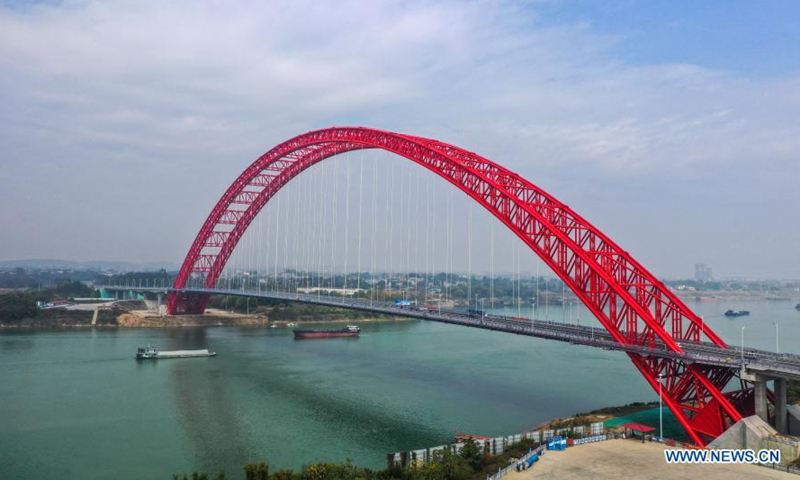
\includegraphics[height = 3.5cm]{/mosty_wstep/photos/pingnan_third_bridge.jpeg} \label{fig:arch_bridges_a}}\;
	\subfloat[Bayonne Bridge\\(fot. Jim Henderson)]{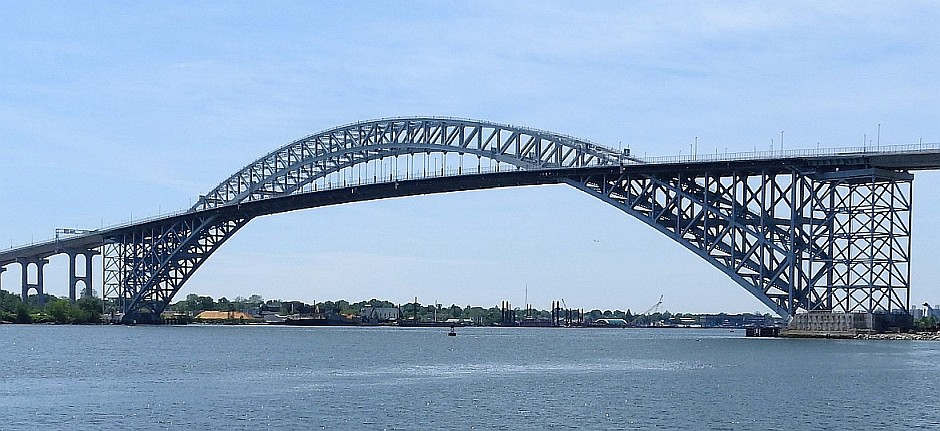
\includegraphics[height = 3.5cm]{/mosty_wstep/photos/High_BB_from_Bayonne_jeh_croped.jpg} \label{fig:arch_bridges_b}}\\
	\subfloat[Most im. gen. Elżbiety Zawackiej\\(fot. Wikipedia User: Pko)]{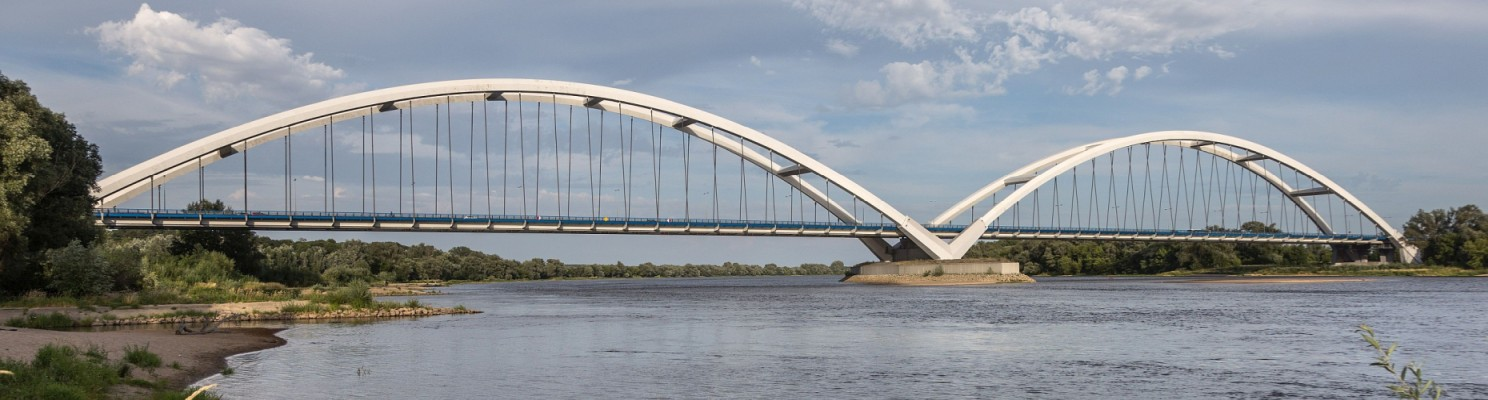
\includegraphics[width = 13.7cm]{/mosty_wstep/photos/Torun_most_Zawackiej_croped.jpg} \label{fig:arch_bridges_c}} \\

	
	\caption{Rekordowe mosty łukowe świata i Polski}
	\label{fig:arch_bridges}
\end{figure}


\subsubsection{Połączenie pomostu i dźwigara łukowego}
Kiedy pomost znajduje się ponad dźwigarem, połączenie pomiędzy pomostem, a dźwigarem łukowym realizuje się za pomocą ścian lub słupków. Kiedy pomost należy podwiesić do dźwigara stosowane są wieszaki. Tradycyjnie łączniki w obu wariantach są ukształtowane jako pionowe. Liczba łączników przyjmowana jest zwykle jako parzysta, tak by klucz łuku znajdował się pośrodku odstępu między wieszakami \parencite{Szczygie1978}. W przypadku konstrukcji z jazdą górą odstępstwa od pionowego ukształtowania słupków zastosował między innymi Morandi (Rys. \ref{fig:bridges_morandi}). 

\begin{figure}[hbt!]
	\centering
	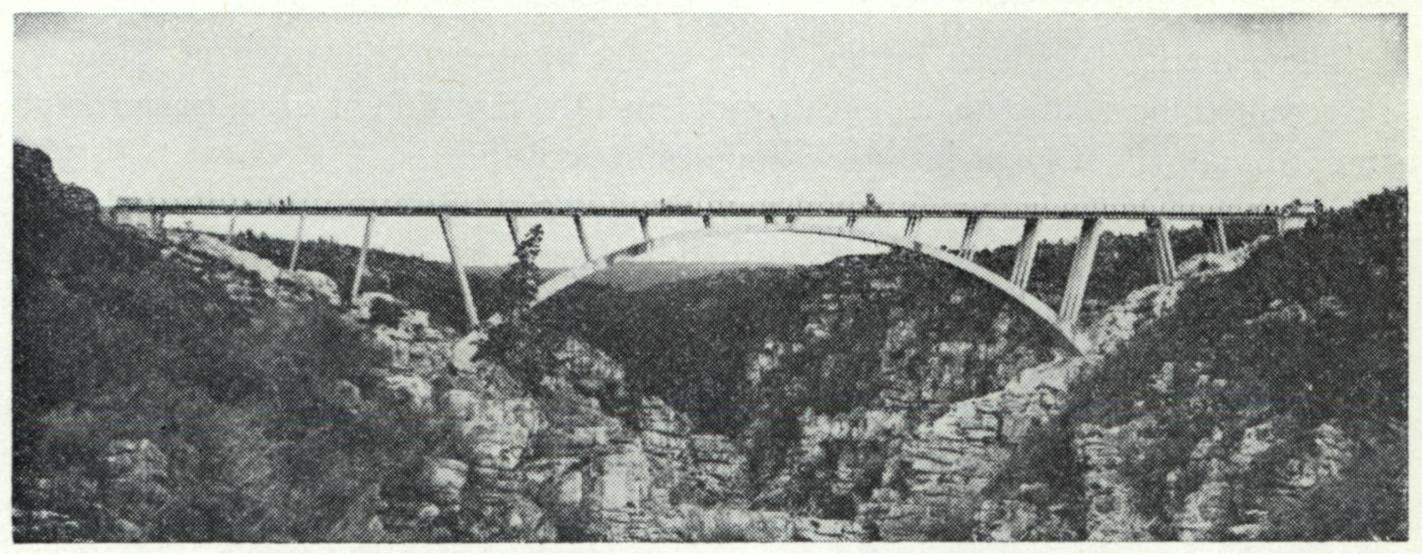
\includegraphics[]{/mosty_wstep/photos/Morandi-works.jpg}
	\captionsetup{justification=centering}
	\caption{Paul Sauer Bridge - most betonowy z jazdą gorą i słupkami ukośnymi. Projektant: Riccardo Morandi \parencite{Morandi1962}}
	\label{fig:bridges_morandi}
\end{figure}

W przypadku obiektów z jazdą dołem występują trzy główne schematy rozkładu wieszaków:
\begin{itemize}
	\item wieszaki proste (Rys. \ref{fig:bridges_types_hangers_a}, \ref{fig:arch_deck_bridges_c}, \ref{fig:arch_deck_bridges_d}),
	\item wieszaki ukośne - Nielsena (Rys. \ref{fig:bridges_types_hangers_b}, \ref{fig:arch_deck_bridges_g},  \ref{fig:arch_deck_bridges_h}),
	\item wieszaki typu Network (Rys. \ref{fig:bridges_types_hangers_c}, \ref{fig:arch_deck_bridges_e}, \ref{fig:arch_deck_bridges_f}).
\end{itemize}

\begin{figure}[h]
	\centering
	\subfloat[wieszki proste]{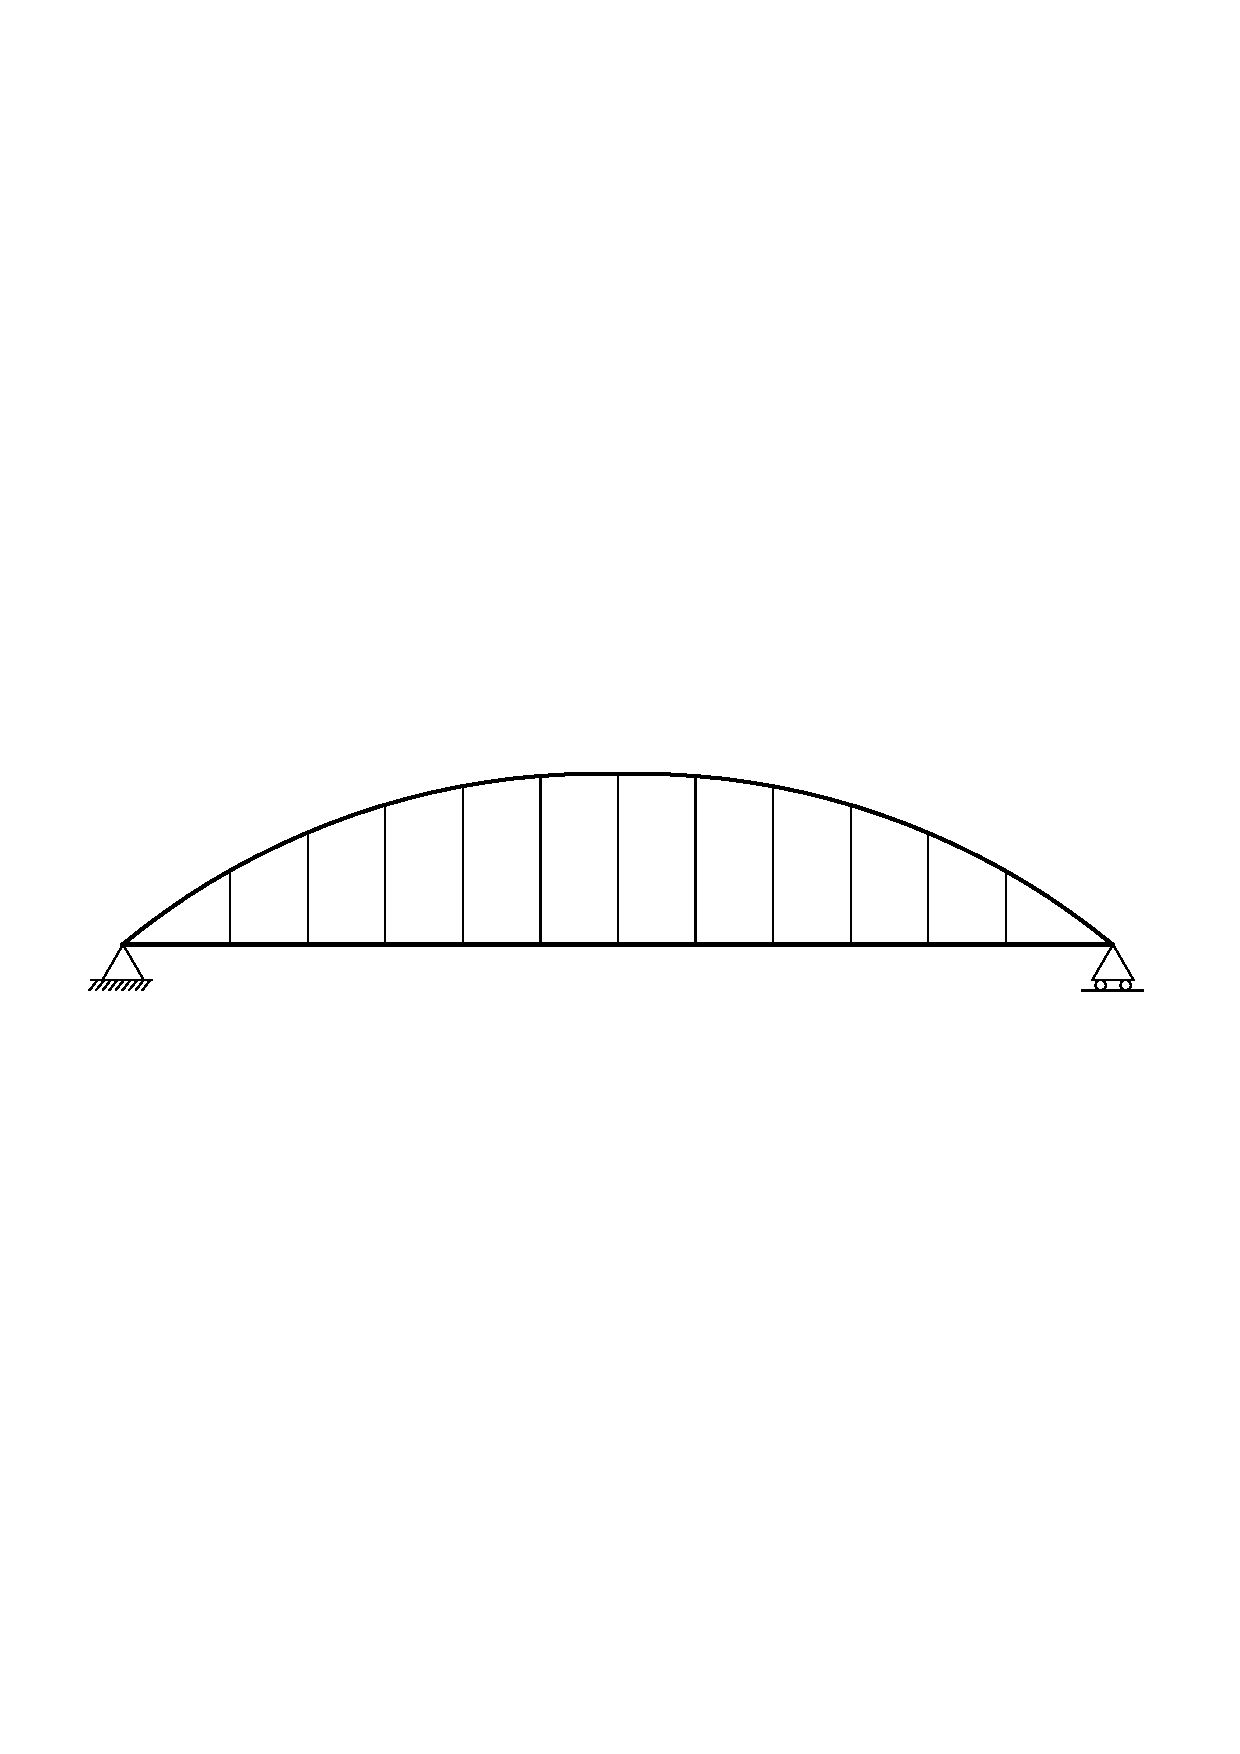
\includegraphics[width=0.7\linewidth,page=1]{/mosty_wstep/mosty.pdf} \label{fig:bridges_types_hangers_a}}  \\
	\subfloat[wieszaki ukośne]{\includegraphics[width=0.7\linewidth,page=2]{/mosty_wstep/mosty.pdf} \label{fig:bridges_types_hangers_b}} \\
	\subfloat[wieszaki typu Network]{\includegraphics[width=0.7\linewidth,page=3]{/mosty_wstep/mosty.pdf} \label{fig:bridges_types_hangers_c}}
	\captionsetup{justification=centering}
	\caption{Układy statyczne mostów łukowych ze ściągiem różniących się układem wieszaków}
	\label{fig:bridges_types_hangers}
\end{figure}

Wieszaki proste są tradycyjnym rozwiązaniem. Względem pozostałych typów charakteryzują się przede wszystkich prostotą wykonania i znacznie mniejszą sztywnością globalną przęsła. System wieszaków ukośnych został zaproponowany przez Octaviusa F. Nielsena w roku 1926. Przyczynkiem do opracowania tego rozwiązania było zjawisko wyłączania się niektórych wieszaków prostych przy obciążeniu ruchomym. W systemie Nielsena nie przewidziano przecinania się wieszaków, a jedynie nachylenie ich pod kątem. Ewolucję tego rozwiązania zaproponował w roku 1955 Per Tveit w swojej pracy magisterskiej. W tym wariancie niektóre z wieszaków przecinają się przynajmniej dwukrotnie \parencite{Tveit2019}. W Polsce funkcjonuje angielska nazwa tego systemu - \textit{Network}. Autor \cite{Tveit2019} jako największą zaletę korzystania z wieszaków typu Network podał, że zapewniają najmniejszą smukłość i lekkość konstrukcji spośród wszystkich wariantów konstrukcji łukowych. Wynika to z większej - w porównaniu do innych systemów - sztywności globalnej konstrukcji, a w konsekwencji powstają mniejsze ugięcia w przęśle i mniejsze obroty na podporach.

\todo{Opis pracy statycznej cięgna. Zostawić czy wywalić?}
W warunkach idealnych podstawowym schematem pracy wieszaka jest osiowe rozciąganie. W rzeczywistości istnieją jednak również inne obciążenia działające na wieszaki, zaburzające stan osiowego rozciągania. Sa to przede wszystkim \parencite{Zobel2015}:
\begin{itemize}
	\item obciążenie poprzeczne od ciężaru własnego (system Nielsena i Network),
	\item obciążenie wiatrem,
	\item wpływ imperfekcji montażowych,
	\item nierównomierna zmiana temperatury,
	\item obciążenie oblodzeniem,
	\item wzbudzenia dynamiczne od drgań konstrukcji i zmian ciśnienia powietrza podczas przejazdu,
	\item ryzyko wyboczenia przy ściskaniu.
\end{itemize}

Elementem strukturalnym, który predestynowany jest do pracy w stanie osiowego rozciągania jest cięgno. Pomimo, że schemat statyczny konstrukcji łukowej najczęściej zakłada przegubowe połączenie pomiędzy wieszakami i dźwigarem w rzeczywistości stosowane są rozwiązania mniej lub bardziej spełniające to założenie. Dwie skrajności stanowią wieszaki sztywno (Rys. \ref{fig:bridges_hangers_fixed}) i przegubowo (Rys. \ref{fig:bridges_hangers_pinned}) połączone z dźwigarem. 

\begin{figure}[hbt!]
	\centering
	\captionsetup{justification=centering}
	\subfloat[]{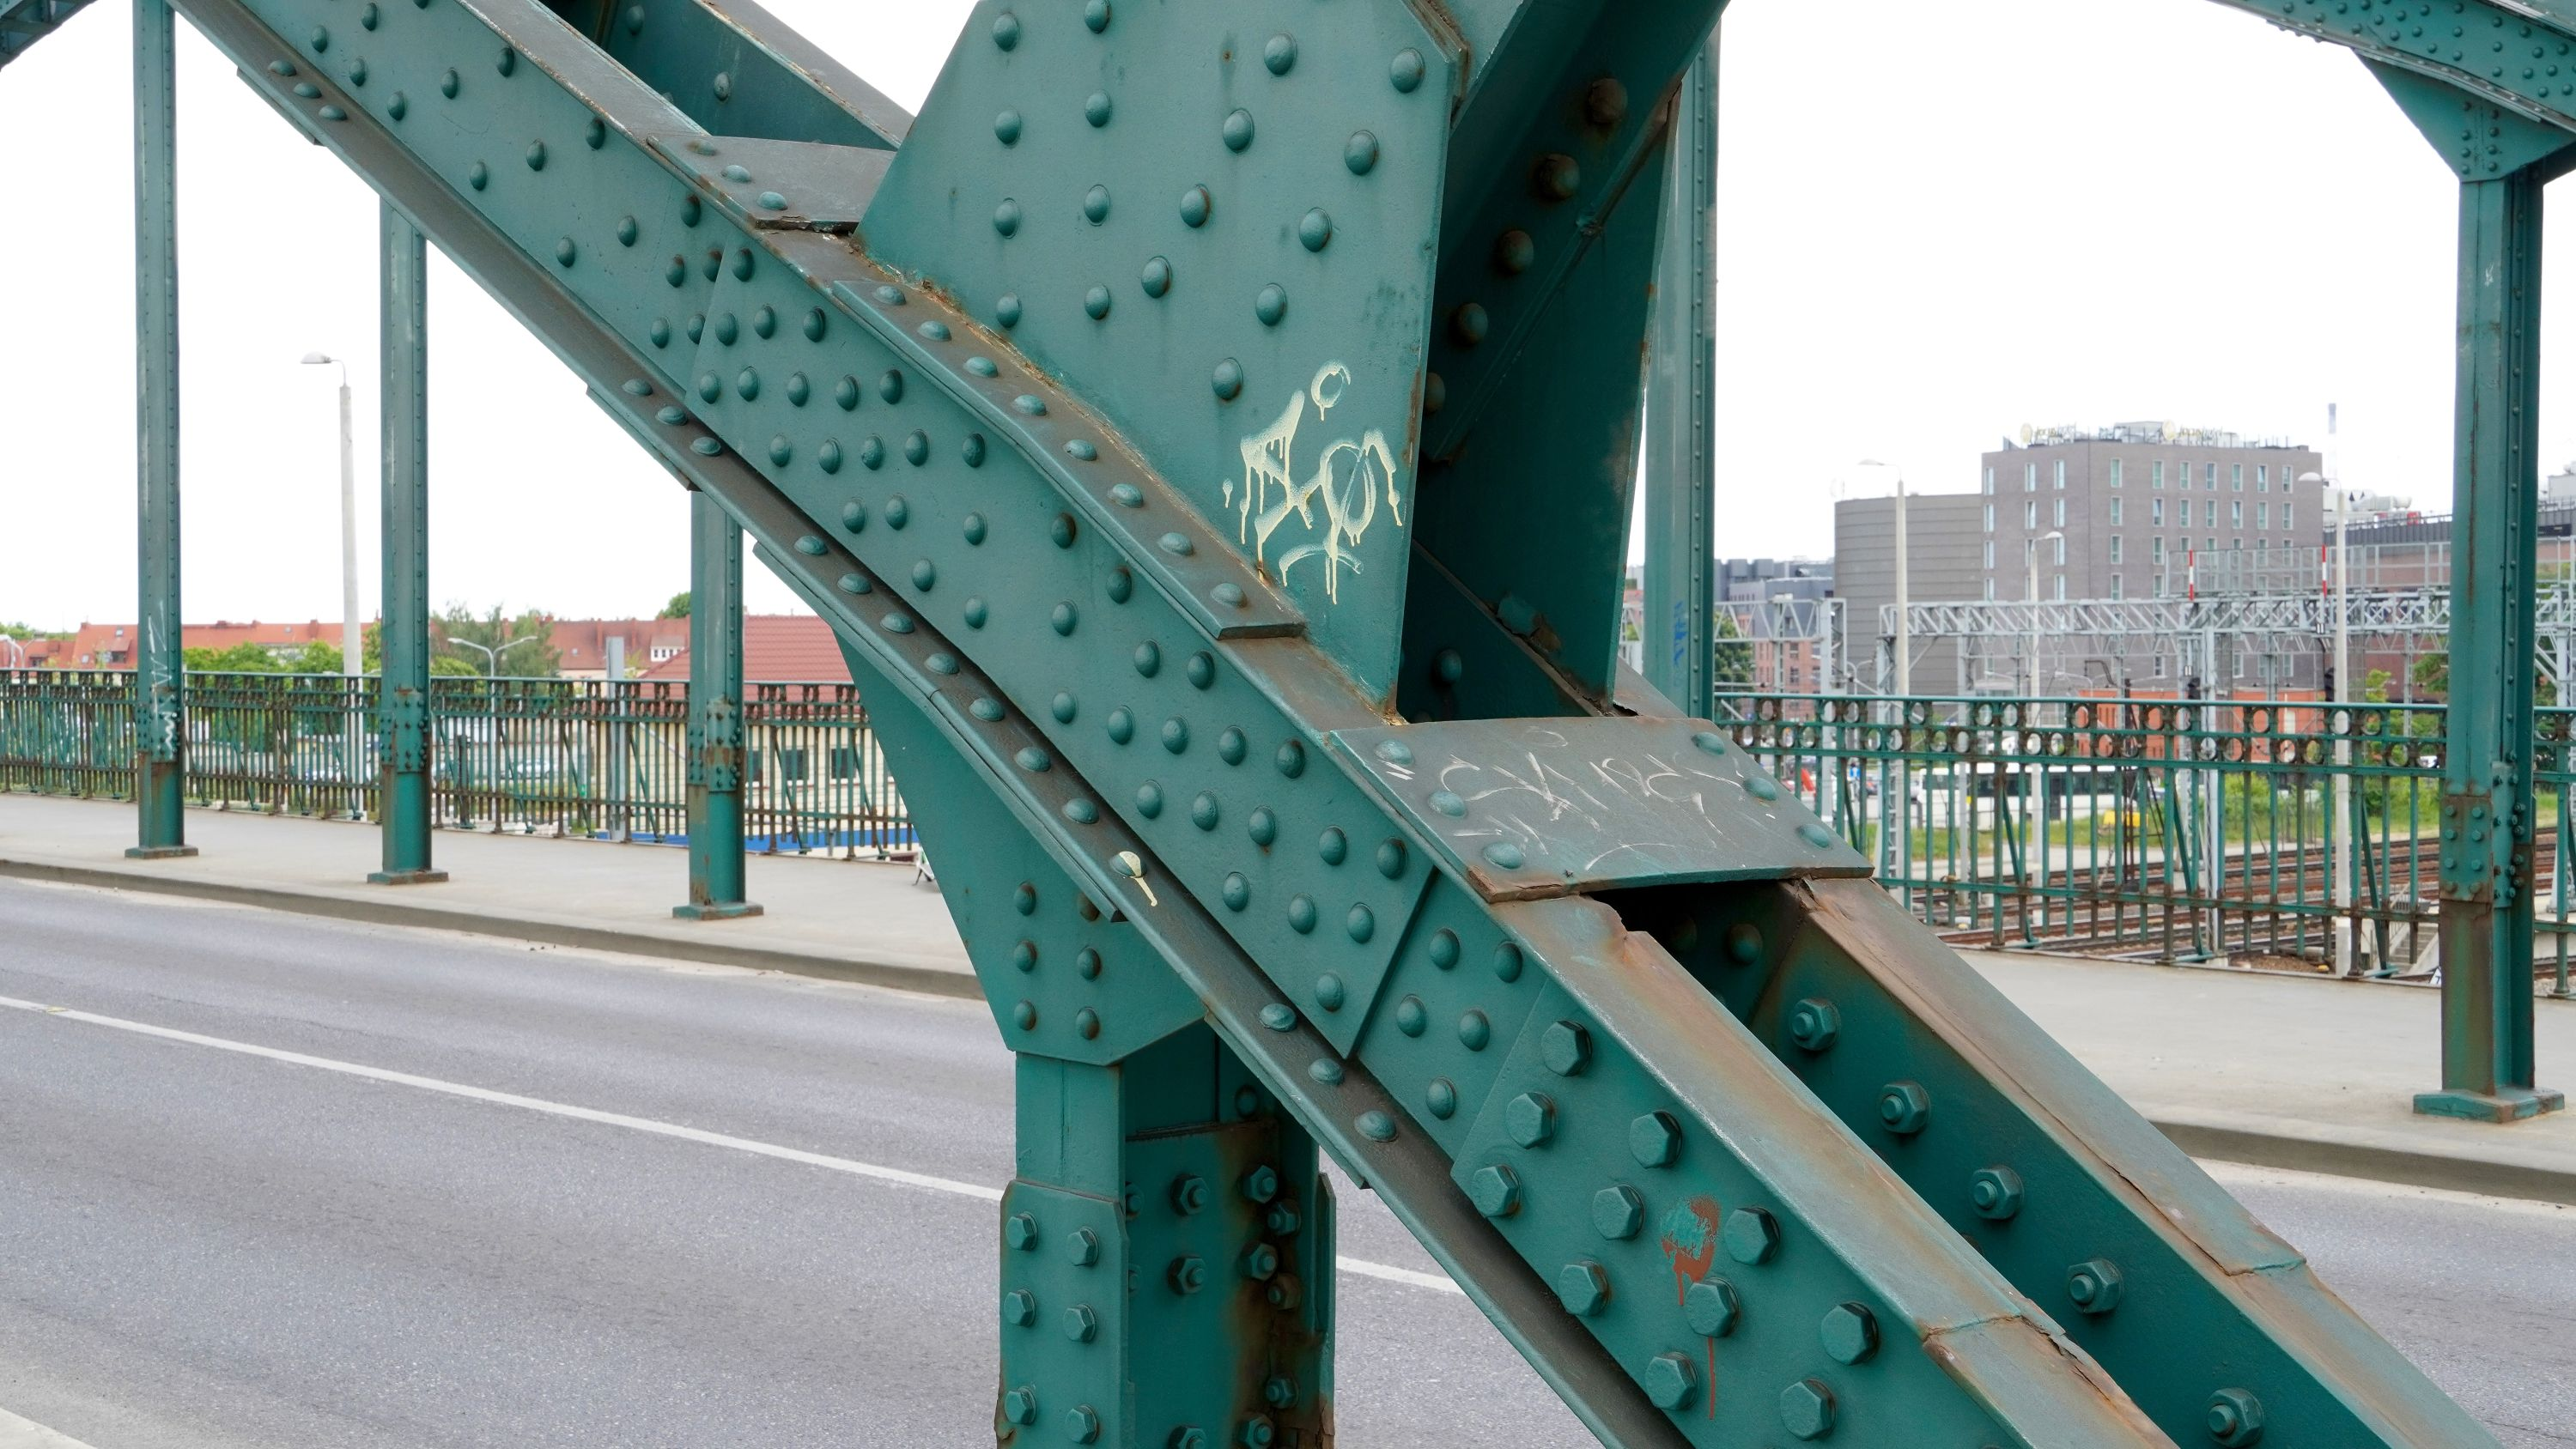
\includegraphics[width=0.48\linewidth]{/mosty_wstep/wieszaki/fot_wieszak_sztywny.jpg} \label{fig:bridges_hangers_fixed}}
	\subfloat[]{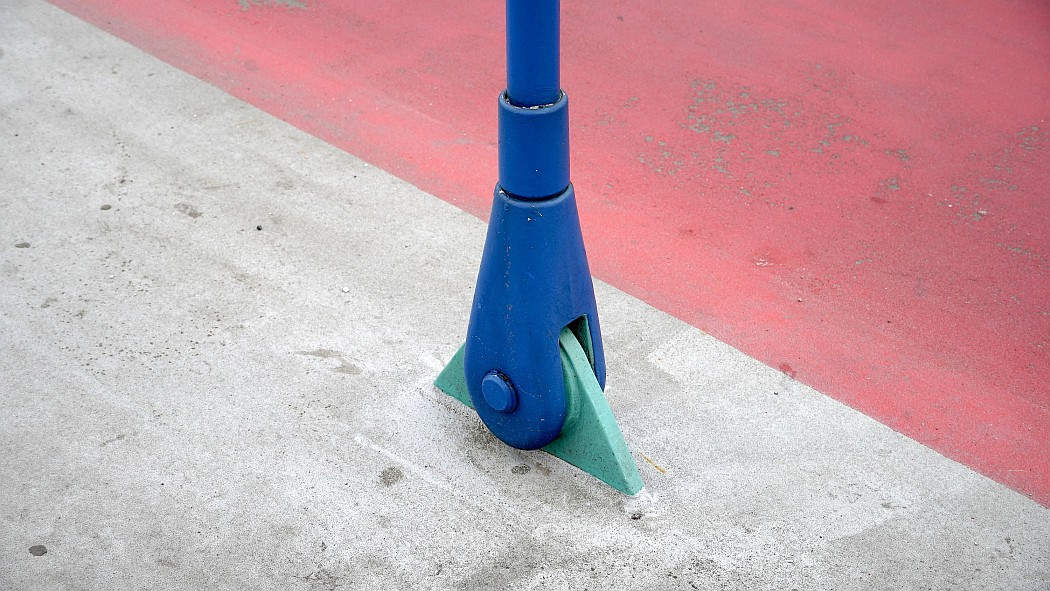
\includegraphics[width=0.48\linewidth]{/mosty_wstep/wieszaki/fot_wieszak_przegub.jpg} \label{fig:bridges_hangers_pinned}}	
	\caption{Przykłady zamocowania wieszaków do dźwigara łukowego: (a) połączenie sztywne, (b) połączenie przegubowe (arch. własne)}
	\label{fig:bridges_hangers_exp}
\end{figure}

Sztywne połączenie może wystąpić dla wieszaków posiadających istotną sztywność giętną (Rys. \ref{fig:bridges_hangers_fixed}) lub na tyle wiotkich, że sztywność giętna jest pomijalna. Pierwsze wykonywane są z profili pełnościennych stalowych lub z betonu \higg{zbrojonego}. W przeszłości wykorzystywano właśnie takie rozwiązanie, ponieważ niemożliwe lub nieracjonalne technologiczne było wykonanie wieszaków cięgnowych. Z taką sytuacją można spotkać się na przykład w łukowych mostach nitowanych (Rys. \ref{fig:arch_deck_bridges_e}  - w tle) z pierwszej połowy XX w. Obecnie \higg{sztywne} wieszaki wykorzystywane są kiedy konstrukcja wymaga usztywnienia poprzecznego łuku, na przykład w przypadku braku stężeń górnych. Należy pamiętać, że w takim przypadku obliczeniowo struktura odbiega w swojej pracy od schematu statycznego łuku i przybliża się do kratownicy Vierendeela. Sztywno połączone z konstrukcją mogą być również wieszaki prętowe o małej sztywności giętnej. Wykonywane są najczęściej jako spawane do blach węzłowych. Rozwiązanie to ma uzasadnienie przede wszystkim ekonomiczne - jest tańsze niż rozwiązania systemowe wieszaków przegubowych. Jednakże ze względu na złożony stan naprężeń w połączeniu należy zwrócić szczególną uwagę na zalecenia konstrukcyjne i technologiczne \parencite{Gunther2000,BundesanstaltfurWasserbauHg.2018,Szafranski2017}. 

Drugą obszerną grupę rozwiązań stanowią wieszaki połączone przegubowo z konstrukcją. Elementy połączone w ten sposób z reguły są wiotkie i traktowane jako cięgna. Obecnie stosowane są następujące typy wieszaków cięgnowych:
\begin{itemize}
	\item pręty okrągłe (Rys. \ref{fig:bridges_hangers_cs_a}),
	\item liny standardowe (Rys. \ref{fig:bridges_hangers_cs_b}) i zamknięte (Rys. \ref{fig:bridges_hangers_cs_c}),
	\item wiązki drutów równoległych lub splotów (Rys. \ref{fig:bridges_hangers_cs_d}), z indywidualnymi lub zbiorczymi zakotwieniami.
\end{itemize}

\begin{figure}[hbt!]
	\centering
	\captionsetup{justification=centering}
	\subfloat[]{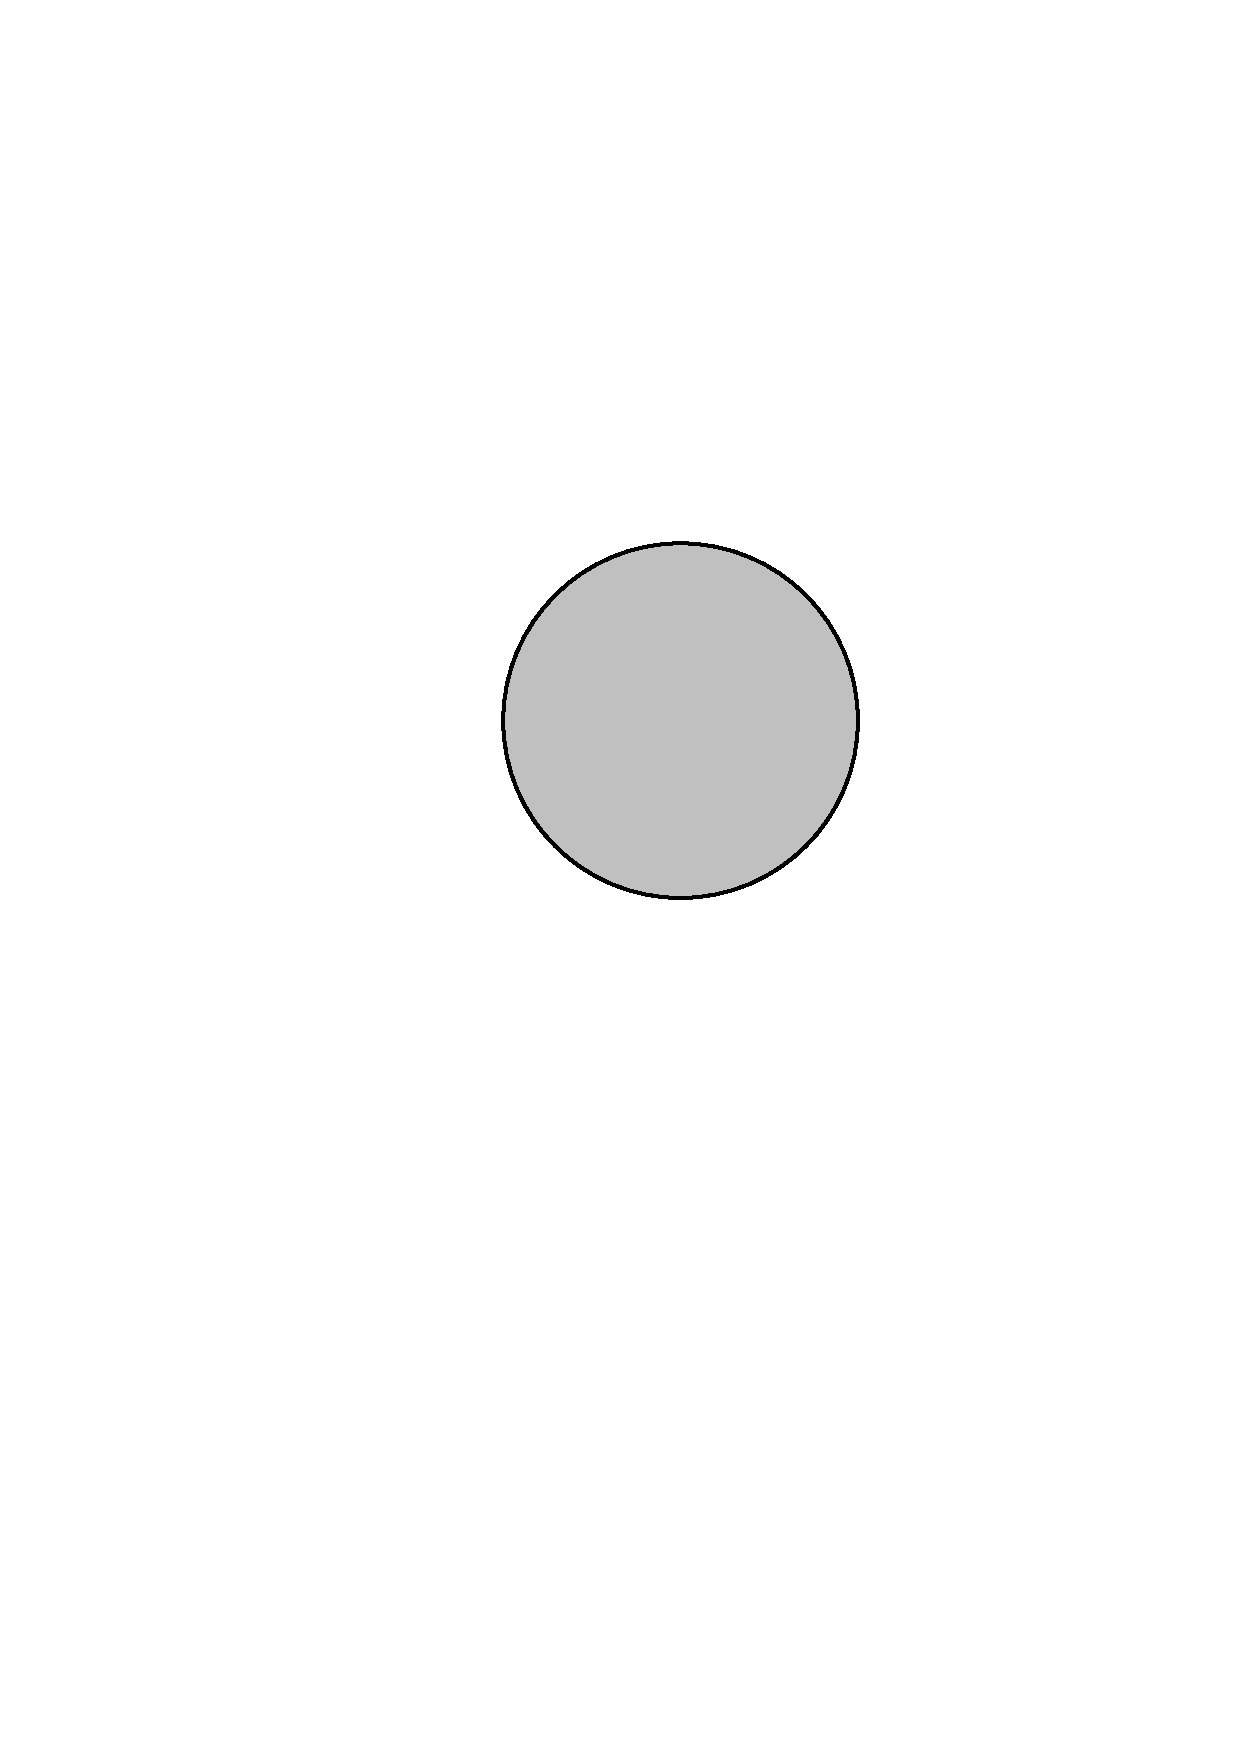
\includegraphics[height=3cm,page=1]{/mosty_wstep/wieszaki/przekroje_wieszaki.pdf} \label{fig:bridges_hangers_cs_a}} \quad
	\subfloat[]{\includegraphics[height=3cm,page=2]{/mosty_wstep/wieszaki/przekroje_wieszaki.pdf} \label{fig:bridges_hangers_cs_b}} \quad
	\subfloat[]{\includegraphics[height=3cm,page=3]{/mosty_wstep/wieszaki/przekroje_wieszaki.pdf} \label{fig:bridges_hangers_cs_c}} \quad
	\subfloat[]{\includegraphics[height=3cm,page=4]{/mosty_wstep/wieszaki/przekroje_wieszaki.pdf} \label{fig:bridges_hangers_cs_d}}	
	\caption{Przekroje poprzeczne stosowanych typów wieszaków: (a) pręty pełne, (b) lina standardowa, (c) lina o konstrukcji zamkniętej, (d) sploty równoległe}
	\label{fig:bridges_hangers_cs}
\end{figure}

Wieszaki cięgnowe połączone z konstrukcją przegubowo w reguły są częścią prefabrykowanych systemów. Dzięki odpowiedniemu systemowi jakości wykonania potwierdzonemu aprobatą, w trakcie projektowania nie ma konieczności konstruowania i sprawdzania poszczególnych elementów połączenia przegubowego i mechanizmów regulacji. Cięgna dobiera się na podstawie katalogów w zależności od wymaganej nośności. Ma to istotne znaczenie zwłaszcza w kontekście wymogów normowych. W zakresie normy \parencite{PN-EN-1993-1-112008} dotyczącej projektowania konstrukcji cięgnowych mieszczą się wszystkie wymienione wyżej typy cięgien połączonych przegubowo. Norma ta przede wszystkim podaje wymagania techniczne dla cięgien, potrzebne do zapewnienia ich bezpieczeństwa, użytkowalności i trwałości. Oczywiście jest ona spójna z filozofią przedstawioną w Eurokodzie 0 i wyróżnia trzy stany graniczne, które muszą być spełnione przy projektowaniu:
\begin{itemize}
	\item Stan Graniczny Nośności \teng{Ultimate Limit State} - porównanie siły osiowej z nośnością obliczeniową przy rozciąganiu,
	\item Stan Graniczny Użytkowania \teng{Serviceability Limit State} - ograniczenie wartości naprężeń i odkształceń,
	\item Stan Graniczny Zmęczenia \teng{Fatigue Limit State} - sprawdzenie zakresów zmienności naprężeń.
\end{itemize}
Dodatkowo w normie zapisano wymóg możliwości regulacji naciągu oraz wymiany cięgien. 

\section{Obliczenia konstrukcji za pomocą Metody Elementów Skończonych} \label{sect:MES}
Metody analityczne wyznaczania sił wewnętrznych czy też odpowiedzi dynamicznej konstrukcji nie mają już wiodącego zastosowania przy rozwiązywaniu rzeczywistych problemów inżynierskich. Model matematyczny oparty na równaniach różniczkowych może być rozwiązany w postaci zamkniętej jedynie w przypadku relatywnie prostych przypadków. Wiele z rzeczywistych układów charakteryzuje się skomplikowanym kształtem, niejednorodnym materiałem, bądź złożonymi warunkami brzegowymi i nie istnieją dla nich rozwiązania ścisłe. Do analizy takich przypadków opracowano znacznie bardziej uniwersalne metody przybliżone, oparte na procesie dyskretyzacji. W \cite{Rakowski2016} autorzy definiują dyskretyzacją jako proces, w którym przekształca się opis pola wyrażony za pomocą nieskończenie wielu parametrów, w opis wyrażony przez skończona liczbę wartości zlokalizowanych w skończonej liczbie punktów (węzłów). Zmienność pola pomiędzy węzłami definiują funkcje kształtu. Istnieją dwie wiodące metody budowy modelu dyskretnego: Metoda Różnic Skończonych (MRS) i Metoda Elementów Skończonych (MES) oraz mniej popularne: Metoda Całkowania Numerycznego (MCN) i Metoda Elementów Brzegowych (MEB). W analizie konstrukcji MES jest zdecydowanie metodą najpopularniejszą, stosowaną w większości programów komercyjnych. W poniższej pracy przy analizie statycznej i dynamicznej posłużono się komercyjnym środowiskiem MES SOFiSTiK w wersji 2018 \cite{SOFISTIK2018,Hartmann2007}. Dla czytelności wywodu, wiadomości o metodach rozwiązywania układów dynamicznych zawarto w rozdziale \ref{sect:dynamic_response_methods}, po przytoczeniu podstawowych informacji o systemach dynamicznych. 

Literatura przedmiotu dotycząca MES jest bardzo rozbudowana. Do podstawowych pozycji opisujących jej rozwój należą \parencite{Kleiber1985,Hughes1987,Zienkiewicz2005,Rakowski2016,Langtangen2019}. Ze względu na obszerność tematu w pracy zaniechano dalszej charakterystyki metody, a skupiono się jedynie na jej zastosowaniu i elementach rozwijających niektóre jej aspekty. Stosowalność MES w analizie konstrukcji została wielokrotnie potwierdzona w literaturze. Autor pracy również wielokrotnie wykorzystywał MES przy rozwiązywaniu rzeczywistych problemów inżynierskich. W następujących pracach opisano niektóre z nich, w których autor brał czynny udział wykorzystując metody numeryczne analizy konstrukcji \parencite{Zotowski2016d,Zotowski2017a,Cudny2017,Zotowski2017h,Zotowski2018a,Zotowski2018d,Zotowski2018c,Binczyk2020a}.

Pomimo długiej historii rozwoju i wielokrotnie potwierdzonej stosowalności MES w analizie konstrukcji zawsze należy pamiętać, że MES jest metodą numeryczną i ma charakter przybliżony. Wynika to z uproszczenia nieskończonego pola w procesie dyskretyzacji i zastosowania funkcji interpolacyjnych. Niedoskonałość metody jest jednym ze źródeł możliwych niedokładności ostatecznego modelu obliczeniowego. Drugie kluczowe przybliżenie wynika z niedoskonałości odwzorowania modelu względem konstrukcji i dotyczy jej kształtu, materiału czy warunków brzegowych. Zagadnienie to zostało szerzej omówione w punkcie \ref{sect:calibration_model}. Istnieją różne metody ograniczenia i kontroli każdego z tych dwóch grup źródeł błędów. W przypadku stosowania elementów dostosowanych\footnote{
	Elementy dostosowane to takie, których funkcje kształtu spełniają wszystkie z trzech kryteriów: kryterium zgodności, kryterium ruchu sztywnego i kryterium stałych odkształceń \parencite{Rakowski2016}}.
błąd wynikający ze stosowania dyskretyzacji i funkcji interpolacyjnych można zmniejszać przez zagęszczenie siatki węzłów (h-convergence) lub poprzez zwiększenie rzędu funkcji interpolacyjnych (p-convergence) \parencite{Zienkiewicz2005}. W poniższej pracy przyjęto pierwszą z nich jako metodę badania zbieżności rozwiązania numerycznego.

\subsection{Kalibracja modeli MES} \label{sect:calibration_model}
Pomimo coraz bardziej intuicyjnych i prostych w użyciu implementacji MES w oprogramowaniu komercyjnym, wciąż wymagane jest od użytkownika doświadczenie i krytyczna ocena wykonywanych obliczeń. Oczywistym jest, że projektant lub badacz chciałby aby stworzony model jak najwierniej odwzorował zachowanie konstrukcji w jego obszarze zainteresowań. Istnieje jednak szereg czynników wpływających na brak zgodności pomiędzy modelem, a konstrukcją. Poza z zasady przybliżonym charakterem obliczeń numerycznych MES, istnieją błędy powstające w procesie modelowania. Można je podzielić na dwie grupy \parencite{Mottershead1993,Mottershead2011}:
\begin{enumerate}
	\item błędy przy tworzeniu modelu i zbytnia idealizacja rzeczywistej konstrukcji przez uproszczone modele mechaniczne,
	\item błędy w przyjęciu parametrów konstrukcji.
\end{enumerate}
\todo{Wyjaśnić punkt 2}

W przypadku analizy konstrukcji budowli, pierwsza grupa obejmuje błędy popełnione przy wykonaniu modelu, takie jak przyjęcie błędnego kształtu, niewłaściwych wartości obciążeń zewnętrznych, braku połączenia między elementami modelu itp. W grupie tej zawrzeć można również błędy założeń teoretycznych, takie jak usztywnienie elastycznych połączeń, brak uwzględnienia wpływu pracy konstrukcji w innych kierunkach niż pionowy, czy też przyjęcie liniowego modelu w przypadku silnie nieliniowej pracy konstrukcji. 

Druga grupa błędów związana jest z niewłaściwym oszacowaniem parametrów modelu. Mogą one skutkować bardzo dużymi różnicami między odpowiedzią konstrukcji rzeczywistej i przewidywaniami modelu. W pracy \cite{Brincker2015} autorzy zestawili możliwe niepewności w oszacowaniu parametrów modeli numerycznych i modalnych co przedstawiono w tabeli \ref{table:uncertainitesModel}). Wartości tych niepewności mogą wynosić od kilku do kilkudziesięciu procent, a w przypadku warunków brzegowych na połączeniu z gruntem trudno wręcz oszacować górną granice. 

\begin{table}[hbt!]
	
	\centering
	\caption{Niepewności najistotniejszych parametrów modeli numerycznych i modalnych na podstawie \cite{Brincker2015}}
	\footnotesize
	\setlength\tabcolsep{0pt}
	%\rowcolors{1}{}{gray!10}
	%\resizebox{\textwidth}{!}{%
		\begin{tabular}{@{}p{0.7\linewidth}  P{0.3\linewidth} @{}}
			\toprule 
			Własność fizyczna  & Poziom niepewności [\%] \\
			\midrule
			Moduł sprężystości i gęstość masy dla stali i innych metali  &    1--5  \\ %\midrule
			Moduł sprężystości i gęstość masy dla betonu, drewna i materiałów zbrojonych włóknami & 5--20\\ %\midrule
			Warunki brzegowe w kontakcie z podłożem gruntowym &    10--$\infty$     \\ %\midrule
			Połączenia śrubowe & 10--$\infty$\\ %\midrule
			Połączenia spawane & 2--10\\ %\midrule
			Masa całkowita & 1--5 \\ %\midrule
			Określana częstotliwość drgań własnych & 0.1--0.05\\ %\midrule
			Pomierzona odpowiedź & 0.2--2\\ %\midrule
			Określane postaci drgań własnych & 2--5\\  %\midrule
			Określane tłumienie & 5--20\\ %\midrule
			Współczynnik skalujący postaci drgań własnych & 5--30\\ 
			\bottomrule
	\end{tabular}
	\label{table:uncertainitesModel}
\end{table}

Redukcja wpływu błędów grupy pierwszej zasadniczo polega na identyfikacji i eliminacji danego błędu. Analizując konstrukcje mostowe stosowane są zabiegi służące wykryciu popełnionych nieprawidłowości. Należą do nich relatywnie proste testy takie jak:
\begin{itemize}
	\item badanie symetrii/antysymetrii efektu obciążenia w przypadku symetrii/antysymetrii układu i obciążenia,
	\item wykonanie analizy modalnej w celu wykrycia miejsce kinematycznych (niepowiązanych elementów modelu) \parencite{Szafranski2013a}, 
	\item sprawdzenie zgodności sumy reakcji z wartością przyłożonego obciążenia. 
\end{itemize}


Niepewności dotyczące parametrów modelu są naturalne i nieodzowne. Podstawowym zadaniem twórcy jest jak najwierniejsze rzeczywistości przyjęcie wartości wielkości fizycznych co niekiedy jest niezwykle trudne i wymaga dużej wiedzy oraz doświadczenia. Jedną z metod na poprawę wartości parametrów jest ich  identyfikacja poprzez badania in situ. W ten sposób można określić na przykład parametry materiałowe lub właściwości podłoża gruntowego. Druga metoda ma charakter pośredni i polega na jak najlepszym dopasowaniu wybranych wartości odpowiedzi modelu do odpowiadających wartości odpowiedzi konstrukcji rzeczywistej. Zestaw procesów prowadzących do tego dopasowania nazywa się kalibracją modelu numerycznego \teng{model updating}. 

Metody \higg{kalibracji} opierają się głównie na modyfikacji parametrów modelu. W pracy \cite{Batou2019} autor podzielił metody \higg{kalibracji} na bezpośrednie - modyfikujące macierz sztywności lub mas - i pośrednie - modyfikujące parametry geometryczne, materiałowe i warunki brzegowe. Za zmianę charakterystyk modelu mogą odpowiadać algorytmy o różnym stopniu skomplikowania. Najbardziej podstawowym jest modyfikacja wybranych atrybutów metodą prób i błędów. \todo{Skreślić całość czy tylko część}\higr{W tym przypadku wyboru, które wartości i w jakim stopniu zmienić dokonuje badacz na podstawie doświadczenia.} Jest ona skuteczna w przypadku układów o relatywnie niewielkich niepewnościach i niewielu parametrach, a także wymaga sporego doświadczenia. Kiedy liczba parametrów jest duża lub bardzo duża stosowanie metody prób i błędów jest nieefektywne. Z tego względu w pierwszym kroku ogranicza się liczebność zmiennych na podstawie rankingu istotności wpływu parametrów na dopasowanie. Pozostawiane do modyfikacji są jedynie te zmienne, które najbardziej wpływają na zmianę odpowiedzi modelu. Najpopularniejszą metodą selekcji jest wykorzystanie analizy wrażliwości \parencite{Friswell2001,Mottershead2011,Petersen2017,Batou2019}.  Kiedy liczba parametrów wciąż pozostaje znacząca, wykorzystywane są metody podziału na mniejsze podproblemy \parencite{Weng2020,Yu2016}. 

W kalibracji stosowane są również metody optymalizacji globalnej, takie jak metoda przeszukiwania lub algorytmy metaheurystyczne, z których najpopularniejsze to algorytm genetyczny (AG) i optymalizacja rojem cząstek (PSO) \parencite{Boulkaibet2015,Tran-Ngoc2018,Dan2015,Qin2018}. Charakteryzują się one zadowalającą efektywnością nawet przy bardzo dużej liczbie zmiennych. W pracy do kalibracji modelu wykorzystano ostatnią z przedstawionych metod, opartą na algorytmie PSO. Informacje na jej temat przedstawiono w rozdziale \ref{sect:PSO_chapter}.

Warto zwrócić uwagę, że kalibracja modelu za pomocą zmiany parametrów, przy jednoczesnym występowaniu błędów z grupy pierwszej, może prowadzić do doboru wartości parametrów o zupełnie nierealnych wielkościach. Stąd też przed przystąpieniem do analizy należy najpierw w miarę możliwości wyeliminować wszystkie błędy związane z tworzeniem modelu i jego zbyt daleko idącymi uproszczeniami.

Kalibracja modelu jest wykorzystywana w wielu rzeczywistych zastosowaniach. Podstawowym celem jest maksymalne dopasowanie modelu do konstrukcji rzeczywistej w trakcie badań naukowych \parencite{Li2020,Brownjohn2001,Zhang2019,Kuzawa2012,Petersen2017,Poprawa2017}. Przygotowany, dobrze odwzorowujący rzeczywistość model może posłużyć do oceny nie tylko jakościowej, ale i ilościowej badanych zjawisk. Kalibracja służy również do oceny stanu konstrukcji i jej zmian, często w połączeniu z systemem monitoringu \parencite{Brownjohn2000,Brownjohn2003,Zoltowski2020}. Działania te najczęściej ukierunkowane są na poszukiwanie i identyfikację uszkodzeń istniejących konstrukcji.



\section{Dynamiczne obciążenie kolejowe}
Ryzyko nadmiernych drgań mostów kolejowych jest rozpatrywane od samych początków budowy dróg szynowych w Anglii na początku XIX w \parencite{Ladislav1996}. Historię badań nad tym zjawiskiem przedstawił w pracy doktorskiej Szafranski \cite{Szafranski2013}, opierając się na obszernych studiach literatury. Podsumowując doświadczenia naukowców i inżynierów, wystąpienie niebezpiecznych amplitud drgań mostów związane jest przede wszystkim ze zjawiskiem rezonansu. W pracy pominięto sytuacje wyjątkowe jak wykolejenia i uderzenia pociągów w elementy konstrukcyjne i skupiono się na typowej eksploatacji mostów. Rezonans mechaniczny może wystąpić w przypadku kiedy pojawia się obciążenie cykliczne, którego częstotliwość oddziaływania pokrywa się z częstotliwością drgań własnych konstrukcji. Kiedy obciążenie jest długotrwałe i w układzie nie ma tłumienia amplitudy drgań mogą teoretycznie rosnąć w nieskończoność. Oczywiście w rzeczywistych konstrukcjach nie mam możliwości nieograniczonego wzrostu amplitud, ponieważ tłumienie układu występuje zawsze, a czas oddziaływania obciążeń ruchomych jest skończony. Niemniej jednak konstrukcje mostowe charakteryzują się zazwyczaj niewielką wartością tłumienia, a obciążenia kolejowe mogą charakteryzować się stosunkowo długim czasem oddziaływania o stałej częstotliwości wymuszenia. W połączeniu z ciągłym rozwojem zarówno taboru kolejowego jak i dróg szynowych, problem wprowadzenia mostu kolejowego w drgania ewoluuje i wymaga od inżynierów ciągłej pracy badawczej.


\subsection{Oddziaływania dynamiczne taboru na mostach kolejowych}
W trakcie bogatej historii badań nad interakcją taboru kolejowego i konstrukcji mostów rozpoznano kilka oddziaływań charakteryzujących się cyklicznością i długim czasem działania, co spełnia znamiona wystąpienia ryzyka rezonansu \parencite{Fryba2001}. Warto zaznaczyć, że ryzyko to nie dotyczy jedynie oddziaływań pionowych, ale również poprzecznych do osi toru. Opisując kompleksowo zagadnienie należy rozpocząć od historycznych oddziaływań, niewystępujących już z uwagi na rozwój techniki. Pierwszym z nich był efekt niedokładnego wyważenia kół osi napędowych lokomotywy parowej. Koło takie posiada przeciwwagę dla elementów połączenia z wiązarami łączącymi koło z osią silnikową. W przypadku braku idealnego wyważenia, koło takie oddziałuje na szynę dodatkową sinusoidalną siłą. Drugie historyczne oddziaływanie było związane z występowaniem połączeń szyn na obiekcie mostowym. Równo i blisko rozstawione koła przejeżdżające przez przerwę połączenia szyn wywoływano cykliczne uderzenie i w konsekwencji drgania całej konstrukcji. To oddziaływanie również nie występuje już w rzeczywistości, ponieważ obecne przepisy zabraniają stosowania złączy szynowych na obiektach inżynieryjnych \parencite{PKPPolskieLinieKolejoweS.A.2005}. \todo{Wezykowanie?}

Spośród obecnie występujących oddziaływań pierwszą przyczyną występowania nadmiernych drgań mogą być duże i wciąż rosnące prędkości eksploatacyjne pociągów. Przy równomiernym lub niemal równomiernym rozstawie osi \higg{lub wózków} i przy stałej prędkości przejazdu, siły przekazywane przez koła na szyny pojawiają się okresowo na obiekcie. Istnieje więc ryzyko, że przy rozstawie osi \higg{lub wózków} $d$ i przy prędkości taboru $c$ czas potrzebny na pojawienie się kolejnych osi na obiekcie $t$ będzie równy okresowi drgań $T_i$. Okres $T_i$ odpowiada częstotliwości drgań własnych konstrukcji $f_i=\frac{1}{T_i}$. Jednakże wzbudzenie może nastąpić również dla wielokrotności (lub ułamka) $k$ okresu drgań. W takim przypadku kolejne siły przykładane są do obiektu co $k$-te wychylenie konstrukcji z położenia równowagi. Prędkość związana z niekorzystną koincydencją $t=kT_i$ nazywana jest prędkością krytyczną \teng{critical speed}. Równaniem (\ref{eq:critical_speed_1}) opisano równość czasu $t$ i okresu $T_i$ grożącą wystąpieniem rezonansu:
\begin{equation} \label{eq:critical_speed_1}
	t=\frac{d}{c}=\frac{k}{f_i}=T_i \quad\text{dla}\quad
	\begin{matrix*}[l]
		i=1,2,3\dots\ \\
		k=1,2\dots,1/2,1/3,\dots
	\end{matrix*}
\end{equation}
Na podstawie równania (\ref{eq:critical_speed_1}) wyznaczyć można prędkość krytyczną $c_{cr}$:
\begin{equation} \label{eq:critical_speed_2}
	c_{cr}=\frac{df_i}{k}\quad \text{dla}\quad
	\begin{matrix*}[l]
		i=1,2,3\dots\ \\
		k=1,2\dots,1/2,1/3,\dots
	\end{matrix*}
\end{equation}
Częstotliwość pojawiania się kolejnych osi jest oczywiście związana z prędkością $c$ i rozstawem osi $d$. W pracy \cite{Fryba2001} autor podaje również drugą formułę na prędkość krytyczną, której osiągnięcie grozi destabilizacją przęsła. Wzór na tę prędkość wyznaczony dla belki swobodnie podpartej podano następujący:
\begin{equation} \label{eq:criticla_speed}
	c_{cr}=\frac{2lf_j}{j}\quad\text{dla}\quad j=1,2,3\dots\ 
\end{equation}
Jak podaje autor, teoretyczne prędkości powodujące destabilizację przęsła są zbyt wysokie i aktualnie nieosiągalne w praktyce. Jednakże należy je rozważyć w kontekście rozwoju technologicznego transportu \parencite{Ladislav2008}.

Drugim niebagatelnym czynnikiem wpływającym na drgania obiektu mostowego przy przejeździe taboru są nierównomierności jezdni \parencite{Ladislav1996,Dias2008}. Są one nieuniknione i wynikają ze zużycia elementów nawierzchni, luzów, osiadania czy niewłaściwego utrzymania. Objawiają się przemieszczeniem wewnętrznych krawędzi szyn od idealnej, projektowanej geometrii. Dla danego punktu wzdłuż osi toru rozróżnia się cztery typy nierównomierności:
\begin{itemize}[noitemsep]
	\item nierównomierność wysokościowa:
	\begin{itemize}
		\item średnia zmiana wysokości osi toru,
		\item różnica wysokości toków szynowych,
	\end{itemize}
	\item nierównomierność poprzeczna:
	\begin{itemize}
		\item średnie przesunięcie poprzeczne osi toru,
		\item zbliżenie/oddalenie się toków szynowych.
	\end{itemize}
\end{itemize}
Nierównomierności wysokościowe wpływają głównie na pionowe drgania konstrukcji, a poprzeczne na poziome i skrętne. Każdy z typów może mieć charakter cykliczny lub losowy. 

Nierównomierności cykliczne opisane mogą być za pomocą szeregów Fouriera \parencite{Ladislav1996}. Inną metodą ich opisu jest użycie gęstości widmowych mocy wyliczonych na podstawie odpowiedzi zmierzonych w trakcie przejazdów testowych \parencite{Claus1998,Dias2008}. Metoda wykorzystująca szeregi Fouriera pozwala również na opisanie jako nierównomierności toru innych, rzeczywistych zjawisk takich jak wypłaszczenie powierzchni tocznej obręczy kół \parencite{Zhou2020} czy efekt zmiany sztywności jezdni na poprzecznicach i podkładach w pomoście z jezdnią otwartą \parencite{Fryba1999}. 

Drgania poziome mogą być związane z siłami podłużnymi lub poprzecznymi. Pierwsze z nich wynikają głównie z przyspieszenia bądź hamowania taboru na moście. Drgania poprzeczne związane są głównie z bocznymi ruchami pojazdu. Mają one swoje źródło głównie w nierównomiernościach poprzecznych toru, mechanizmie wężykowania \parencite{Babe2016}, deformacjach konstrukcji w skutek mimośrodowego obciążenia obiektu i występowaniu siły odśrodkowej \parencite{Dias2008}. Na rysunku \ref{fig:railway_dynamic_forces} przedstawiono schemat podsumowujący rzeczywiste oddziaływania dynamiczne taboru kolejowego na mosty.
\begin{figure}[hbt!]
	\centering
	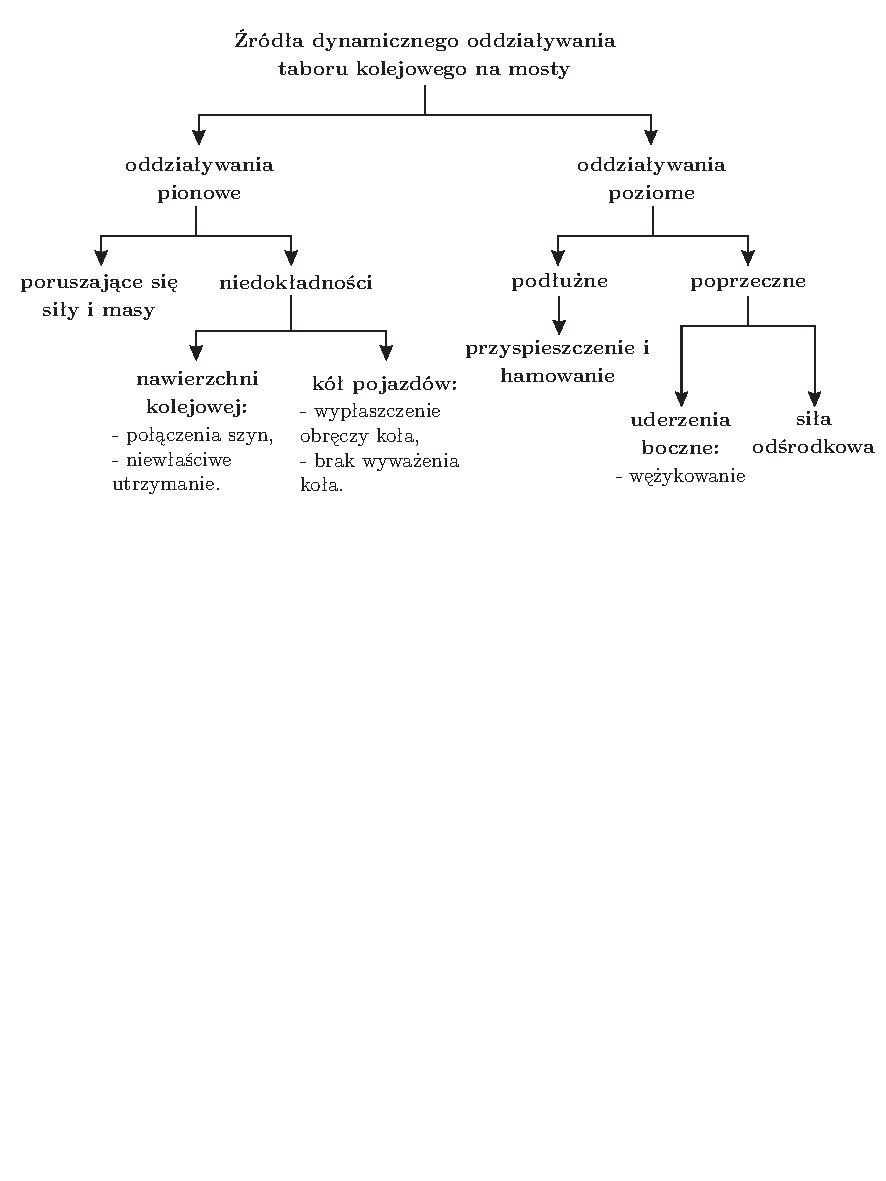
\includegraphics[width=\textwidth]{/dynamic_railway/railway_bridges_forces_croped.pdf} 
	\captionsetup{justification=centering}
	\caption{Zestawienie efektów dynamicznych działających na konstrukcję mostu w trakcie przejazdu taboru kolejowego (na podstawie \parencite{Ladislav1996})}
	\label{fig:railway_dynamic_forces}
\end{figure}


%Pierwsze z nich utożsamiane jest z normowym Stanem Granicznym Nośności, a drugie ze Stanem Granicznym Użytkowania \parencite{rho_{min}}. 


\subsection{Efekty dynamiczne w mostach kolejowych} \label{sect:railway_dynamic_effects}
\todo{Wyjaśnić uwagę}
Obecnie rozważania dotyczące oddziaływań taboru na mostu kolejowe skupiają się przede wszystkim na obiektach projektowanych \higg{na Liniach} Dużych Prędkości. Oczywiście od wielu lat w przypadku wszystkich \higg{obiektów} kolejowych w trakcie projektowania należy sprawdzić dwa główne kryteria: wytrzymałości i trwałości zmęczeniowej konstrukcji oraz bezpiecznego i komfortowego użytkowania. Pierwsze z nich utożsamiane jest z normowym Stanem Granicznym Nośności, a drugie ze Stanem Granicznym Użytkowania \parencite{PKNc}. W ramach pierwszego sprawdzane są zwykle wytrzymałość materiałów, stateczność i deformacje konstrukcji oraz wykonywane są analizy zmęczeniowe \parencite{Ladislav2008}. Drugie kryterium jest znacznie bardziej złożone i restrykcyjne w przypadku mostów w ciągu LDP. Poza relatywnie prostym w zrozumieniu komfortem pasażera, wymaga ono sprawdzenia bezpieczeństwa nawierzchni kolejowej na moście. Zakłada się, że nawierzchnia jest bezpieczna jeśli jest stabilna i wskutek przejazdu nie nastąpi ryzyko zerwania kontaktu pomiędzy szyną i kołem \parencite{Ramondenc2008}. Przy \higg{prawidłowo} utrzymywanym torze, utrata stabilności nawierzchni może nastąpić przede wszystkim w przypadku rozluźnienia podsypki. Pierwszy raz z tym problemem zetknięto się w trakcie utrzymania obiektów mostowych w ciągu trasy francuskiego TGV \parencite{Ramondenc1998}. Zauważono, że tor wymagał znacznie częstszych niż zwykle prac konserwacyjnych. Przeprowadzono badania, w których wykazano, że przy przyspieszeniach pionowych większych niż $0.7g-0.8g$ następuje efekt rozluźnienia podsypki i utrata jej stabilności przez zmniejszenie sił tarcia pomiędzy ziarnami kruszywa \parencite{Zacher2008}. Niestateczność podsypki może skutkować zmniejszeniem siły w styku koła i szyny, a w skrajnym wariancie wykolejeniem się pociągu. Kolejnym czynnikiem mogącym wpłynąć na zaburzenie styku koła z szyną są zmiany geometrii toru wywołane przejazdem taboru po obiekcie. W zależności od typu konstrukcji, schematu statycznego, liczby torów zagadnienie to może różnić się stopniem skomplikowania. Niebezpieczne deformacje mogą wynikać z ugięcia wspornika za osią podparcia mostu, z obrotu konstrukcji na łożysku wskutek ugięcia przęsła, ze skręcenia toru po długości obiektu czy ze zmiany krzywizny w planie. Dodatkowo z uwagi na możliwość wystąpienia rezonansu pomiędzy drganiami poprzecznymi mostu i pojazdem szynowym ogranicza się minimalną częstotliwość poprzecznych drgań własnych mostu \parencite{Goicolea2003,Dias2007,Dias2008}. W pracy 
\parencite{Niemierko} autor podaje, że już na etapie projektowania należy rozważyć następujące wartości związane z bezpieczeństwem i komfortem przejazdu pojazdu szynowego:
\begin{itemize}
	\item przyspieszenia przęsła,
	\item pionowe ugięcia pomostu,
	\item reakcje (uniemożliwić odrywanie na łożyskach),
	\item przemieszczenia wspornika przęsła poza osią podparcia,
	\item kąty skręcenia przęsła,
	\item kąty obrotu na łożyskach,
	\item przemieszczenia wzdłuż osi podłużnej mostu,
	\item ugięcie w poprzek mostu,
	\item kąt obrotu przęsła w poziomie,
	\item częstotliwości drgań własnych konstrukcji.
\end{itemize}

Uwzględnienie efektów dynamicznych przy projektowaniu i w ocenie mostów może odbywać się na wiele sposobów. Obecnie odbywa się to na dwa główne sposoby \parencite{Goicolea2008a}:
\begin{enumerate}
	\item przez zwiększenie odpowiednim współczynnikiem dynamicznym\footnote{
		Dyskusję na temat nazewnictwa dotyczącego różnicy pomiędzy przemieszczeniami statycznymi i dynamicznymi, a w tym m.in.: \enquote{współczynnik dynamiczny}, \enquote{współczynnik nadwyżki dynamicznej} i \enquote{współczynnik przewyższenia dynamicznego} w kontekście projektowania i próbnych obciążeń przeprowadzono w pracy \parencite{Poprawa2018}} 
	efektów oddziaływań statycznych od obciążeń ruchomych,
	\item przez wyznaczenie i ocenę odpowiedzi dynamicznej układu pod obciążeniem ruchomym.
\end{enumerate}

Od wielu lat polskie jak i zagraniczne normy posługują się współczynnikiem dynamicznym do uwzględnienia efektów dynamicznych przy projektowaniu mostów \parencite{Karas2011}. Metoda polega na zwiększeniu efektów oddziaływania pochodzącego od statycznych modeli obciążeń kolejowych, tak żeby uwzględnić nadwyżkę wynikającą z dynamiki przejazdu po obiekcie. W ten sposób bierze się pod uwagę zarówno wzbudzenie dynamiczne wynikające ze zmienności położenia obciążenia w czasie oraz nierównomierności nawierzchni kolejowej i niedoskonałości kół pojazdów. Należy jednak pamiętać, że podane wzory na wyznaczenie współczynnika dynamicznego zostały wyznaczone dla pojedynczej osi obciążenia ruchomego przejeżdżającego przez obiekt i nie uwzględniają warunków rezonansu \parencite{Goicolea2008}. Jest to uzasadnione rozwiązanie, ponieważ zjawisko rezonansu zwykle nie występuje w sposób istotny przy przejazdach z prędkością mniejsza nić 200 km/h. Dodatkowo współczynnik dynamiczny nie jest stosowany do obciążeń odwzorowujących rzeczywisty tabor tylko do modeli obciążenia będących obwiednią szerokiej klasy obciążeń kolejowych: pociągów pasażerskich, towarowych i specjalnych. Należy więc pamiętać o jego ograniczeniach stosowalności, co zaznaczono w obowiązujących przepisach \parencite{PKNj}. 

Druga rodzina metod opiera się na wyznaczeniu odpowiedzi dynamicznej układu pod wpływem przejazdu przez wykonanie analizy dynamicznej. Metody wyznaczania odpowiedzi różnią się stopniem złożoności i liczbą uwzględnianych czynników \parencite{Goicolea2008a}. Obliczenia mogą odbywać się analitycznie lub za pomocą metod numerycznych. \higg{Pojazd może być opisany jako zestaw sił pozbawionych inercji, jako zestaw mass poruszających się bezpośrednio po układzie lub też jako zestaw oscylatorów lepkosprężystych odwzorowujących również zawieszenie pociągu.} Ostatni wariant może być rozbudowywany do większej liczby stopni swobody i o inne elementy interakcji pomiędzy pojazdem, a konstrukcją \parencite{Calcada2008,Szafranski2013,Szafranski2021}. Uwzględnienie resorowania pojazdu szynowego z reguły obniża efekt wzbudzenia obiektu w trakcie przejazdu. Warto jednak zauważyć, że uwzględnienie interakcji pomiędzy taborem, a konstrukcją nie wpływa \higg{istotnie} na rezultaty analizy dla przypadków bez wystąpienia rezonansu, dla dużych rozpiętości przęseł lub konstrukcji ciągłych \parencite{Goicolea2008a}.

Pierwsze rozwiązania analityczne drgań konstrukcji z obciążeniem ruchomym dla elementarnych modeli mechanicznych pojawiły się już XIX w. Prace \parencite{Willis1849,Stokes1849,Saller1921,Timoshenko1922,Inglis1934,Kolousek1973} stanowią kamienie milowe w historii rozwoju metod wyznaczania odpowiedzi układów mechanicznych pod obciążeniem ruchomym. Tematyka rozwiązań analitycznych nie będzie rozwijana w niniejszej pracy z uwagi na obszerność zagadnień i dostępną literaturę krajową \parencite{Szczesniak2018}. Metody analityczne ograniczone są do raczej prostych modeli elementarnych i typowych obciążeń. Pomimo ich niekwestionowanego wkładu w rozwój badania odpowiedzi dynamicznej mostów oraz ich walory edukacyjne, w pracy posiłkowano się bardziej uniwersalnymi metodami numerycznymi. \higg{Metody analityczne mimo ograniczeń w praktyce są niezbędne do weryfikacji metod numerycznych. Wykorzystuje się je do porównania rezultatów przykładów testowych} \teng{benchmark tests} Warto jednak wspomnieć o jednej z najprostszych, a jednocześnie stosunkowo uniwersalnej metodzie wyznaczenia maksymalnych przyspieszeń za pomocą Dynamicznej Sygnatury Pociągu \teng{Dynamic Train Signature} \parencite{Goicolea2008a,ERRI1998}. Chociaż ma ona zastosowanie jedynie do układu belki wolno podpartej, to jej niewątpliwą zaletą jest, że nie wymaga stosowania złożonych metod numerycznych ani zaawansowanego aparatu matematycznego do uzyskania miarodajnych wyników. W metodzie uwzględnia się charakterystyki dynamiczne układu, dynamiczną linię wpływu mostu \teng{dynamic influence line} oraz sygnaturę dynamiczną pociągu. Wspomniana sygnatura dynamiczna pociągu jest funkcją określoną indywidualnie dla danego pociągu i jest niezależna od cech mechanicznych przęsła. Funkcja zależna jest od typowego rozstawu osi pociągu oraz liczby tłumienia układu. Dzięki wyprowadzonym formułom metoda jest przystępna również dla inżynierów niezajmujących się pracą naukową.

W przypadkach złożonych układów mechanicznych, gdzie metody analityczne nie mają zastosowania, aktualnie najbardziej uniwersalną metodą przewidywania odpowiedzi dynamicznej jest wykorzystanie Metody Elementów Skończonych (p. \ref{sect:MES}). Podstawowe metody przewidywania odpowiedzi systemów dynamicznych opierają się na bezpośrednim całkowaniu numerycznym równań ruchu lub superpozycji modalnej. 

Szerszy opis metod wyznaczania odpowiedzi konstrukcji dla układów o jednym lub wielu stopniach swobody zawarto w rozdziale \ref{sect:dynamic_response_methods}.


\subsection{Przepisy normowe i wytyczne}
Po omówieniu przyczyn, efektów i metod przewidywania drgań konstrukcji należy odnieść się do aktualnego stanu prawnego. Obecnie w Polsce obowiązuje szereg norm i zarządzeń opisujących elementy projektowania, dostosowywania i utrzymania obiektów kolejowych w ciągu Linii Dużych Prędkości \parencite{PKNc,PKNj,PolskieLinieKolejoweS.A.2005,standardytechnicznetomIII,PolskiKomitetNormalizacyjny}. Szczegółową analizę zapisów dotyczących uwzględniania zachowania dynamicznego mostów kolejowych według polskich przepisów opisali w swoich pracach \cite{Oleszek2015,Oleszek2015b,Oleszek2016a}. Aktualnie obowiązujące Eurokody w części poświęconej dynamice mostów kolejowych opierają się na badaniach i doświadczeniach członków Europejskiego Instytutu Badawczego Kolejnictwa (ERRI) \parencite{ERRI1998,Muncke2008}, Międzynarodowego Związku Kolei (UIC) \parencite{UnionInternationaleDesCheminsDeFer2006,UnionInternationaleDesCheminsDeFer2009}. Szczegółową historię ewolucji przepisów do postaci aktualnie występującej w normach europejskich oraz ich interpretację przedstawił w pracy doktorskiej James \cite{James2003}. Również bardzo obszerny opis zagadnienia można znaleźć w \parencite{Dias2007,Goicolea2002}.

W pracy \cite{Karas2011a} autor określił przedstawione w Eurokodach podejście dotyczące uwzględniania efektów dynamicznych  jako kompromis. Z jednej strony w niektórych przypadkach stosuje się tradycyjną metodę zwiększenia efektu oddziaływań statycznych za pomocą współczynnika dynamicznego, z drugiej zaś strony niekiedy wymagane jest stosowanie nowoczesnych metod wyznaczania odpowiedzi konstrukcji pod obciążeniem dynamicznym. Ostatecznie jednak norma nakazuje porównanie efektów obliczeń obiema metodami i uznaje za decydujący przypadek bardziej niekorzystny. 

\subsubsection{Algorytm wyboru zakresu analiz}
W normie PN-EN 1991-2 wyraźnie określono w punkcie 6.4.5.1(1), że współczynnik dynamiczny nie uwzględnia efektów rezonansu. Jednocześnie zdając sobie sprawę z czasochłonności pełnej analizy dynamicznej spróbowano ograniczyć jej wykonanie do przypadków nietypowych i realnie zagrożonych nadmiernymi drganiami. Wprowadzono algorytm decydujący o wyborze metody uwzględnienia efektów dynamicznych. Zastosowano szereg kryteriów, po których spełnieniu można pominąć wyznaczenie odpowiedzi dynamicznej konstrukcji, a efekty przejazdu uwzględnia się za pomocą współczynnika dynamicznego. Algorytm opisujący ścieżkę postępowania zawartą w normie przytoczono za normą \parencite{PKNj} na rysunku \ref{fig:ec_algorithm_dyna}, gdzie: $V$ - miejscowa maksymalna prędkość liniowa [km/h], $L$ - rozpiętość przęsła [m], $n_0$ - pierwsza częstotliwość giętnych, \higg{pionowych} drgań własnych mostu [Hz], $n_T$ - pierwsza częstotliwość skrętnych drgań własnych mostu [Hz], $v$ - maksymalna prędkość nominalna [m/s], $(v/n_0)_{lim}$ - współczynnik wg załącznika F normy. \higg{Liczby w nawiasach okrągłych (1) - (7) umieszczone w blokach algorytmu oznaczają uwagi przytoczone w normie w sąsiedztwie diagramu}. Zgodnie z przedstawionym schematem kluczowymi parametrami potrzebnymi do podjęcia decyzji o wykonaniu analizy dynamicznej są:
\begin{itemize}
	\item maksymalna miejscowa prędkość na linii $V$,
	\item schemat statyczny konstrukcji,
	\item rozpiętość przęsła $L$, 
	\item pierwsza częstotliwość giętnych drgań własnych $n_0$,
	\item pierwsza częstotliwość skrętnych drgań własnych $n_T$
\end{itemize}
\begin{figure}[p]
	\centering
	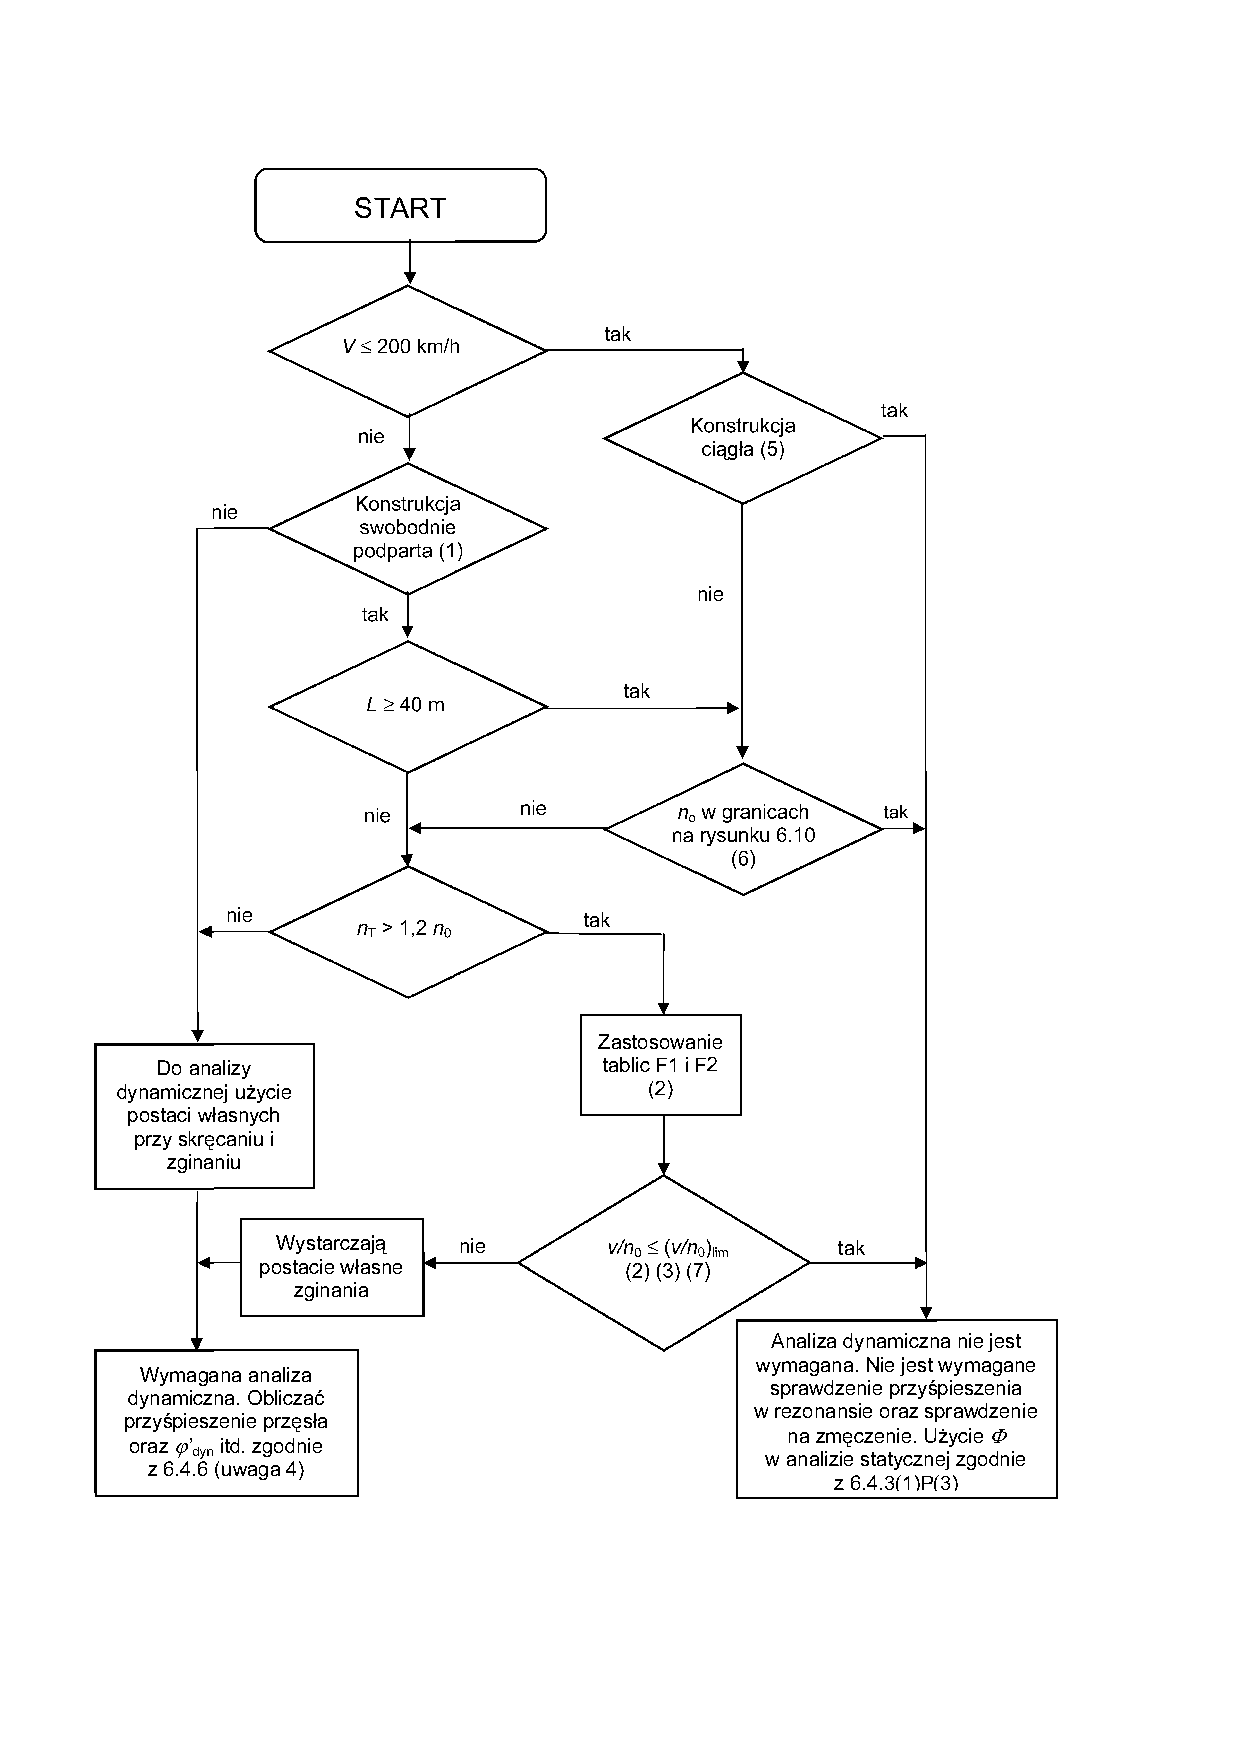
\includegraphics[width=\textwidth]{/dynamic_railway/ec_algorithm_dyna.pdf} 
	\captionsetup{justification=centering}
	\caption{Algorytm określający czy wymagana jest analiza dynamiczna wg \parencite{PKNj}}
	\label{fig:ec_algorithm_dyna}
\end{figure}

Po ustaleniu wszystkich parametrów schemat decyzyjny wskazuje ewentualną konieczność wykonania analizy dynamicznej. Algorytm zależnie od ich wartości realizuje wiele scenariuszy. Można jednak wyodrębnić poszczególne sytuacje, które wynikają z algorytmu i mają potwierdzenie we wcześniej przytoczonych badaniach i opracowaniach dotyczących drgań mostów kolejowych pod obciążeniem ruchomym. Poniżej krótko omówiono kluczowe aspekty mechanizmu decyzyjnego. 

Schemat statyczny wpływa na przebieg procesu wyboru w dwóch miejscach. Po pierwsze konstrukcja może być ciągła lub swobodnie podparta. Po drugie, swobodnie podparte przęsło może różnić się stopniem skomplikowania układu. Roboczo w tej pracy rozróżniono je i nazwano jako konstrukcje \enquote{proste} bądź \enquote{złożone}. Konstrukcja określona jako \enquote{prosta} to zgodnie z normą taka, której schematem statycznym jest \textit{belka swobodnie podparta zachowująca się tylko jak prosta belka podłużna lub prosta płyta z pomijalnymi efektami skosu na podporach niepodatnych}. W przeciwnym wypadku konstrukcja jest \enquote{złożona}.

Do wyznaczenia częstotliwości i postaci drgań własnych niezbędne jest wykonanie analizy modalnej (p. \ref{sect:modal_analysis}). Dla złożonych układów wykonywana jest ona zazwyczaj w programach MES. Dodatkowo, w niektórych sytuacjach proces decyzyjny pozwala pominąć analizę dynamiczną opierając się na nomogramie (rys. \ref{fig:ec_algorithm_dyna_boundary}) oraz Załączniku F do normy PN-EN 1991-2. Nomogram pokazuje obszar stosowalności współczynników dynamicznych w zależności od częstotliwości pierwszej giętnej postaci drgań własnych w funkcji rozpiętości przęsła. Innymi słowy jeżeli pierwsza częstotliwość giętnych drgań własnych obiektu o konstrukcji 'prostej' i danej rozpiętości mieści się pomiędzy dolną, a górną granicą zakreskowanego obszaru, to współczynniki dynamiczne $\phi '$ i $\phi ''$ zdefiniowane przez normę są miarodajne i analiza dynamiczna nie jest wymagana. Granica górna nomogramu jest związana z nierównościami toru, a granica dolna ujmuje dodatkowe oddziaływanie wynikające z samej dynamiki przejazdu. W przypadku prędkości większych niż 200 km/h nomogram ma zastosowanie do dłuższych obiektów \enquote{prostych} ($L\ge 40$ m). Dla mniejszych rozpiętości, przy odpowiednim stosunku częstotliwości drgań skrętnych i giętnych ($n_T>1.2n_0$) możliwe jest pominięcie analizy dynamicznej z wykorzystaniem załącznika F do normy. 
\begin{figure}[hbt!]
	\centering
	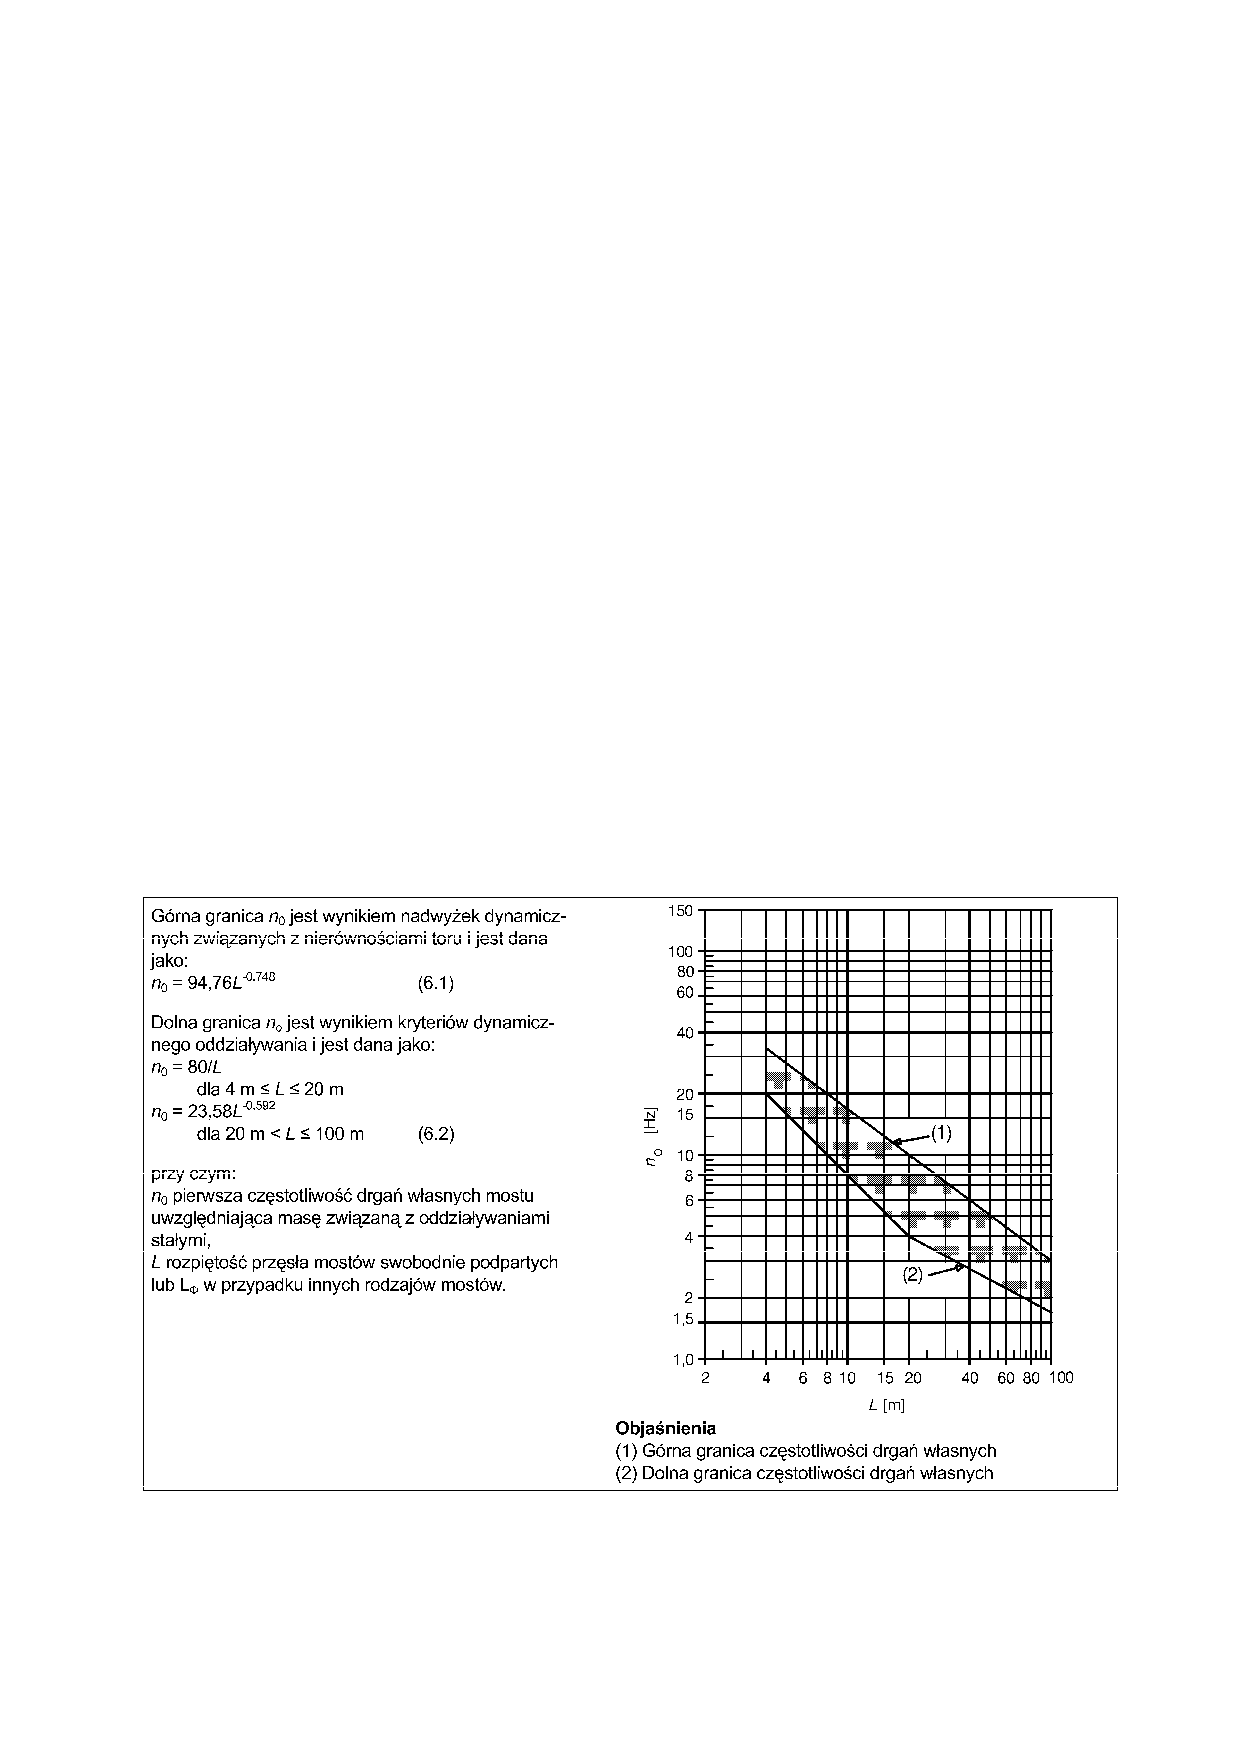
\includegraphics[width=\linewidth]{/dynamic_railway/ec_algorithm_dyna_boundary.pdf} 
	\captionsetup{justification=centering}
	\caption{Granice pierwszej częstotliwości drgań własnych mostu określone w normie \cite{PKNj}, decydujące o konieczności wykonania pełnej analizy dynamicznej}
	\label{fig:ec_algorithm_dyna_boundary}
\end{figure}

W załączniku F zestawiono współczynniki graniczne $(v/n_0)_lim$, gdzie $v$ - maksymalna prędkość nominalna taboru. Współczynniki graniczne zostały zdefiniowane i zestawione w tablicach F.1 i F.2 normy. Wyznaczono je dla 'prostych' obiektów o zróżnicowanych - lecz nieograniczonych - rozpiętościach oraz dla różnych ułamków tłumienia i różnych zastępczych obciążeń równomiernie rozłożonych przypadających na metr bieżący mostu. Według algorytmu jeżeli dla obliczanego obiektu spełnione jest $(v/n_0)>(v/n_0)_{lim}$ to analiza dynamiczna nie jest wymagania, ponieważ efekt obciążenia będzie mniejszy niż przy obciążeniu statycznym LM 71 z odpowiednim współczynnikiem dynamicznym. Wartości graniczne $(v/n_0)_{lim}$ zostały wyznaczone przy uwzględnieniu współczynników bezpieczeństwa dla kryteriów przyspieszenia, ugięcia i wytrzymałości, dla starannie utrzymanego toru i częstotliwości $n_0$ mniejszej niż górna granica nomogramu (rys. \ref{fig:ec_algorithm_dyna_boundary}. Do analiz użyto 7 pociągów rzeczywistych A-F również przedstawionych w załączniku F. 

Nomogram (Rys. \ref{fig:ec_algorithm_dyna_boundary}) oraz tablice w załączniku F, powstały na bazie wielu lat badań i doświadczeń naukowców i inżynierów zajmujących się tematyką drgań mostów kolejowych \parencite{UnionInternationaleDesCheminsDeFer2009,ERRI1998}. Dzięki nim zidentyfikowano przypadki konstrukcji dla których nie ma obowiązku ponownego prowadzenia pełnej analizy dynamicznej. Mimo, że dotyczy to jedynie \enquote{prostych}, powtarzalnych konstrukcji, to w typowych przypadkach pozwala zaoszczędzić projektantom mnóstwo czasu. 


Powyżej wymieniono przypadki kiedy istnieje możliwość zaniechania prowadzenia analiz dynamicznych. Z drugiej strony, przy maksymalnej prędkości większej od 200 km/h analiza dynamiczna musi być wykonana jeśli:
\begin{itemize}
	\item konstrukcja jest \enquote{złożona},
	\item konstrukcja jest \enquote{prosta}, rozpiętość jest mała ($L < 40$ m), a częstotliwość drgań własnych skrętnych jest bliska częstotliwości drgań własnych giętnych ($n_T<1.2n_0$),
	\item konstrukcja jest \enquote{prosta}, rozpiętość jest duża ($L \ge 40$ m), ale częstotliwość giętnych drgań własnych nie mieści się w wyznaczonych granicach (Rys. \ref{fig:ec_algorithm_dyna_boundary}) i częstotliwość drgań własnych skrętnych jest bliska częstotliwości drgań własnych giętnych ($n_T<1.2n_0$).
\end{itemize}




\subsubsection{Obciążenia} \label{sect: eurokod_obciazenia_dyn}
W pracy poruszany jest temat optymalizacji struktury obiektów mostowych, który zdecydowanie częściej może być rozważany na etapie projektowania mostu aniżeli w trakcie jego życia. Z tego względu w dalszej części pracy rozważone zostaną obciążenia służące projektowaniu, a nie sprawdzaniu istniejących konstrukcji. Według rozporządzenia \parencite{PolskiKomitetNormalizacyjny} do projektowania należy używać modeli obciążeń zawartych w omawianej już normie PN-EN 1991-2, a do sprawdzania nośności istniejących obiektów kolejowych modeli obciążeń eksploatacyjnych opisanych w normie PN-EN 15528 \parencite{PolskiKomitetNormalizacyjnya,uszczki2015}. Norma \cite{PolskiKomitetNormalizacyjnya} zawiera instrukcje i przepisy pozwalające zaklasyfikować pojazdy i linie kolejowe do odpowiednich klas.

W normie PN-EN 1991-2 występuje kilka obciążeń kolejowych podzielonych na dwie grupy w zależności od przeznaczenia. Pierwszą grupę stanowią obciążenia do analiz statycznych. W jej skład wchodzą modele obciążenia: UIC 71, SW/0, SW/2 i pociąg bez ładunku. Model UIC 71 został opracowany już w 1971 roku \parencite{UnionInternationaleDesCheminsDeFer2006} i był stosowany również w poprzedniej generacji Polskich Norm \parencite{PKNe}. Z tego względu jest dobrze znany środowisku projektowemu i zwykle nie występują problemy w jego zastosowaniu. Obciążenia statyczne nie stanowią głównego tematu niniejszej pracy i nie będą szerzej omawiane. Ich szczegółowy opis, pochodzenie oraz zasady użycia można znaleźć w normie PN-EN 1991-2 oraz pracach \parencite{James2003,UnionInternationaleDesCheminsDeFer2006}. Druga grupa zawiera modele obciążeń wykorzystywane w analizach dynamicznych lub zmęczeniowych. Zaliczają się do niej:
\begin{itemize}
	\item Pociągi Rzeczywiste (PN-EN 1991-2 załącznik F)
	\item Pociągi Uniwersalne HSLM-A i HSLM-B (PN-EN 1991-2 p. 6.4.6.1.1),
	\item Pociągi Zmęczeniowe\footnote{
		Odniesienie do Pociągów Zmęczeniowych w kontekście analizy dynamicznej znajduje się w punkcie 6.4.6.1.1(7) normy. Mówi on o zalecanych obciążeniach w przypadku kiedy analiza dynamiczna jest wymagana, a maksymalna prędkość jest mniejsza niż 200 km/h. W angielskiej wersji tekstu pojawia się zdanie "Train Types 1 to 12 given in annex D", które wyraźnie odnosi się do Pociągów Zmęczeniowych. W polskiej wersji zdanie to zostało przetłumaczone jako "Pociągi Typowe od 1 do 12 podane w załączniku D". Pojęcie Pociąg Typowy występuje również w załączniku D w odniesieniu do jednego z rodzajów Pociągów Rzeczywistych. Racjonalne wydaje się dosłowne stosowanie przepisu w jego angielskiej formie.} 
	(PN-EN 1991-2 załącznik D). 
\end{itemize}

Opis obciążeń dynamicznych należy rozpocząć od przywołania idei interoperacyjności. Zgodnie z dyrektywą Rady Unii Europejskiej 96/48/WE z 1996 roku opracowano Warunki Techniczne Interoperacyjności \teng{Technical Specifications of the Interoperability (TSI)} \parencite{Muncke2008}. Mają one w założeniu ujednolicić dotychczas zróżnicowane systemy kolejowe państw członkowskich Unii Europejskiej. Dzięki wdrożeniu idei ułatwione ma być podróżowanie pomiędzy krajami Unii, bez utrudnień związanych z zastosowaniem różnych rozwiązań technicznych. Zgodnie z Warunkami TSI wszystkie obiekty kolejowe powinny być zwymiarowane na obciążenie statyczne LM71 oraz pozwolić na Liniach Dużych Prędkości na ruch wszystkich, aktualnie występujących i mogących wystąpić w przyszłości Pociągów Dużych Prędkości.

\higg{Pierwszą grupą obciążeń normowych używanych do analiz dynamicznych są modele odpowiadające pociągom rzeczywistym, tak zwane} \enquote{Pociągi Rzeczywiste}. Pociągi Dużych Prędkości występujące na europejskich LDP mogą być podzielone na trzy typy taboru w zależności od wzajemnego usytuowania wózków i wagonów \parencite{Goicolea2008a}. Schematy \higg{modeli} pociągów zawarto w normie PN-EN 1991-2 załącznik E i przytoczono na rysunku \ref{fig:train_types_EC}. Poszczególne typy można opisać następująco (w nawiasach podano przykłady rzeczywistego taboru):
\begin{itemize} 
	\item pociągi przegubowe - dwa wagony połączone są jednym wózkiem znajdującym się między nimi (THALYS, AVE i EUROSTAR),
	\item pociągi typowe - każdy wagon posiada dwa własne wózki (ICE2, ETR500),
	\item pociągi regularne - brak wózków, wagony są oparte na pojedynczych osiach znajdujących się na połączeniu wagonów (TALGO).
\end{itemize}
\begin{figure}[hbt!]
	\centering
	\subfloat[]{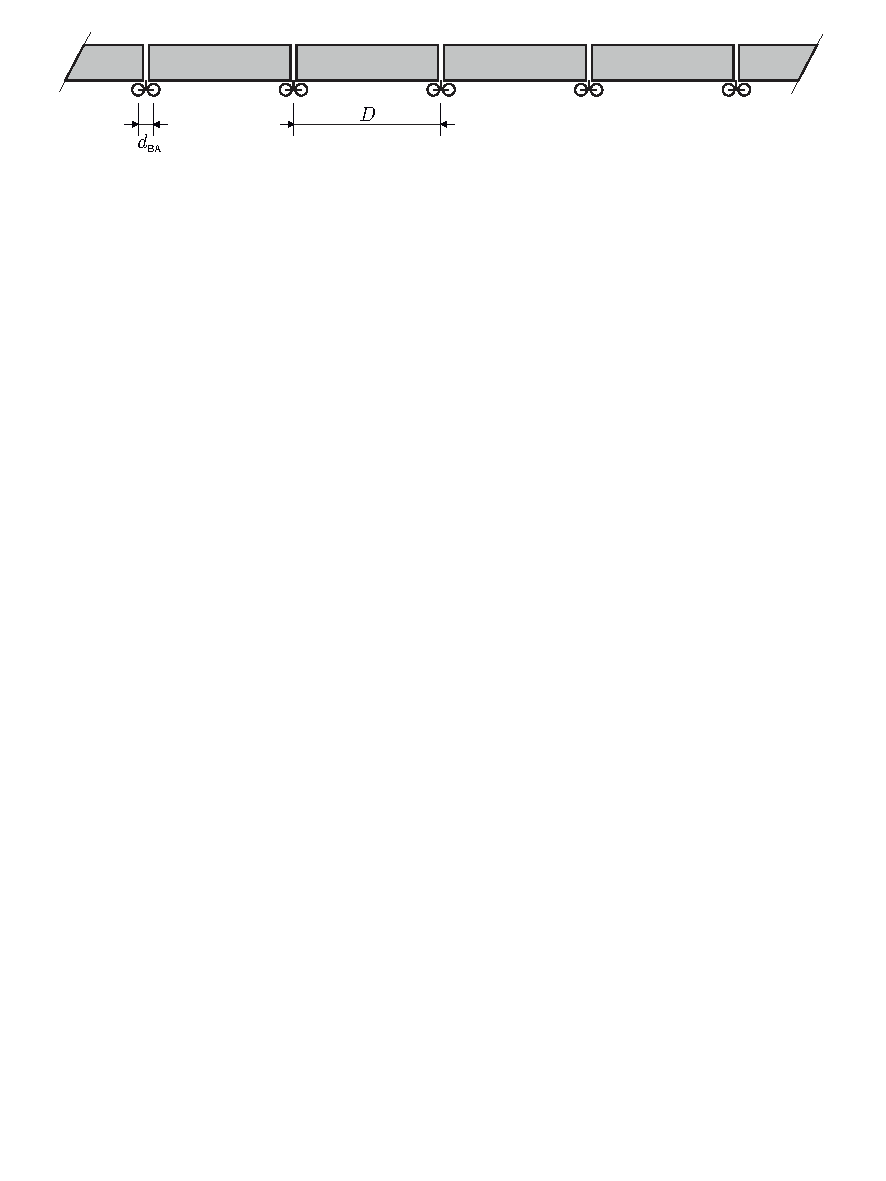
\includegraphics[]{/dynamic_railway/types_of_trains_articulated.pdf}  \label{fig:train_types_EC_art} } \\
	\subfloat[]{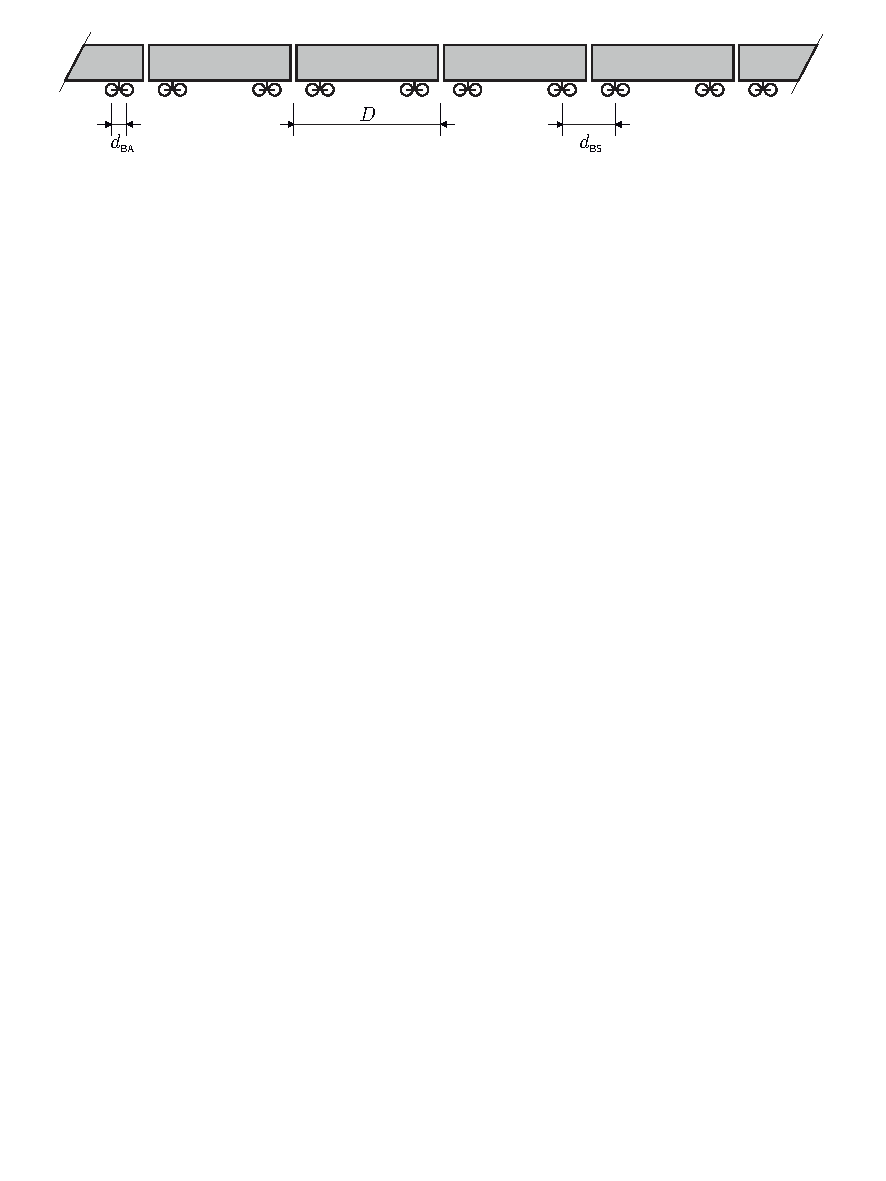
\includegraphics[]{/dynamic_railway/types_of_trains_conventional.pdf}} \\
	\subfloat[]{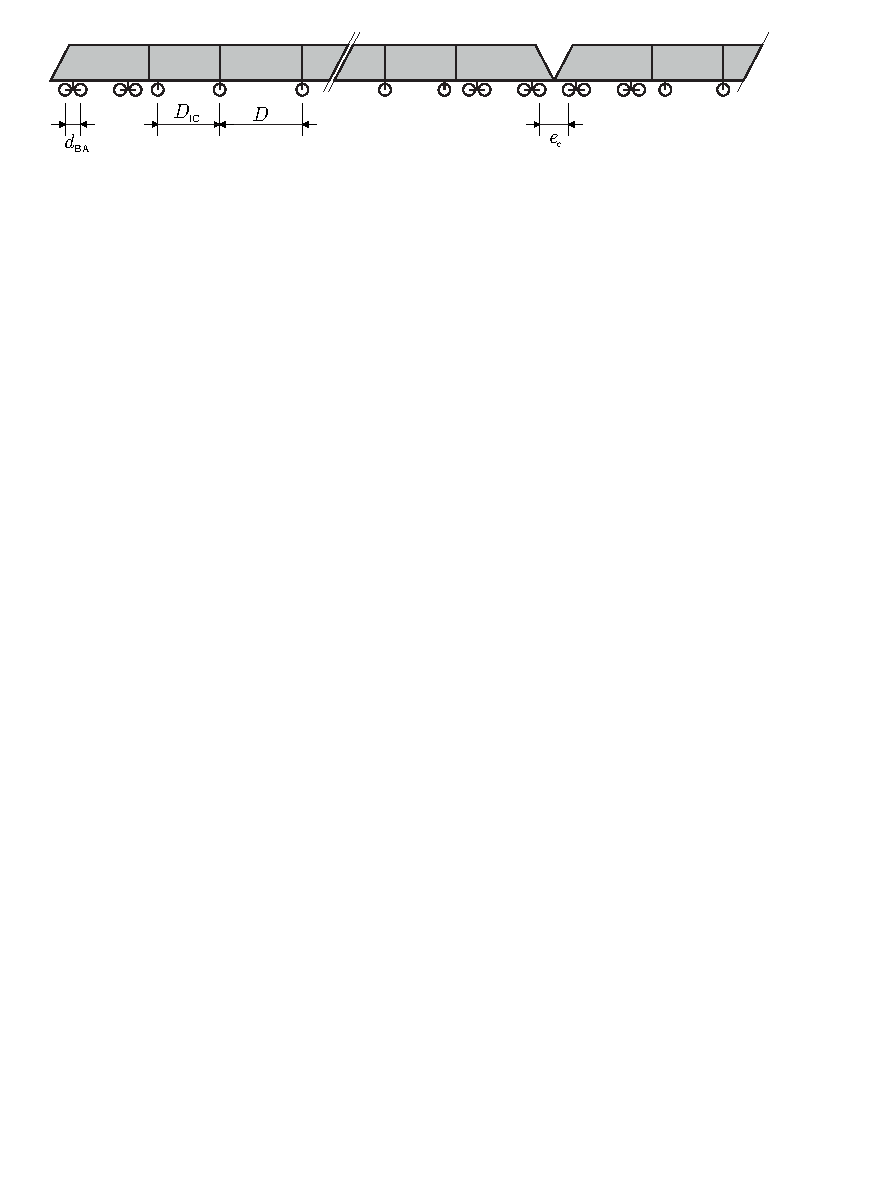
\includegraphics[]{/dynamic_railway/types_of_trains_regular.pdf}}
	\captionsetup{justification=centering}
	\caption{Typy pociągów rzeczywistych kursujących na Europejskich LDP: (a) pociąg przegubowy; (b) pociąg typowy; (c) pociąg regularny. Oznaczenia: $d_{BA}$ - rozstaw osi w wózku, $D$ - odległość miedzy regularnie odległymi osiami lub długość wagonu, $D_{IC}$ - długość wagonu pośredniego, $e_c$ - odległość między sąsiednimi osiami dwóch pojedynczych zestawów pociągów \parencite{PKNj}.}
	\label{fig:train_types_EC}
\end{figure}
Na liniach kolejowych o prędkości maksymalnej mniejszej niż 200 km/h zarządca w indywidualnej dokumentacji technicznej może określić \enquote{Pociągi Rzeczywiste}, które należy uwzględnić w analizach.

\begin{figure}[hbt!]
	\centering
	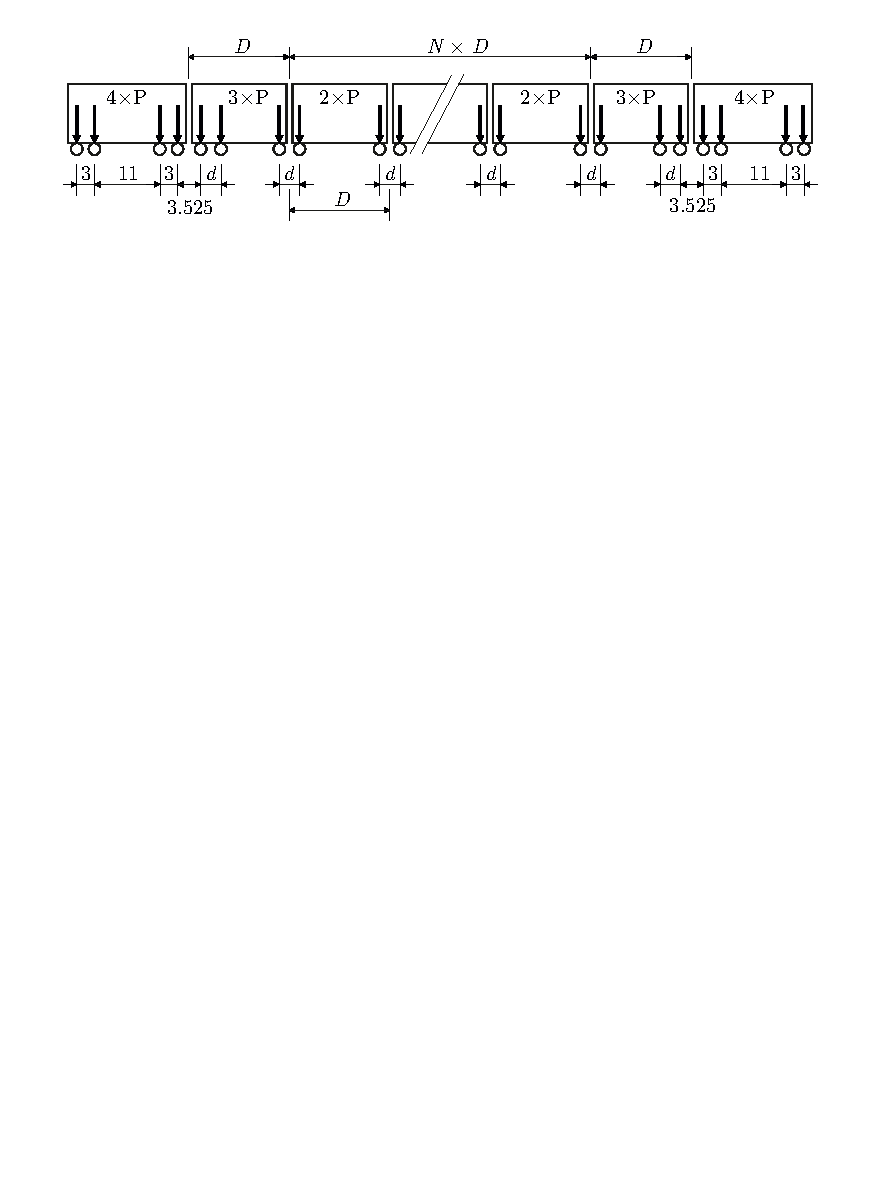
\includegraphics[]{/dynamic_railway/hslm_a.pdf}
	\captionsetup{justification=centering}
	\caption{Model pociagu HSLM-A według PN-EN 1991-2. Na podstawie \cite{PKNj}}
	\label{fig:train_hslm_a}
\end{figure}

\begin{figure}[hbt!]
	\centering
	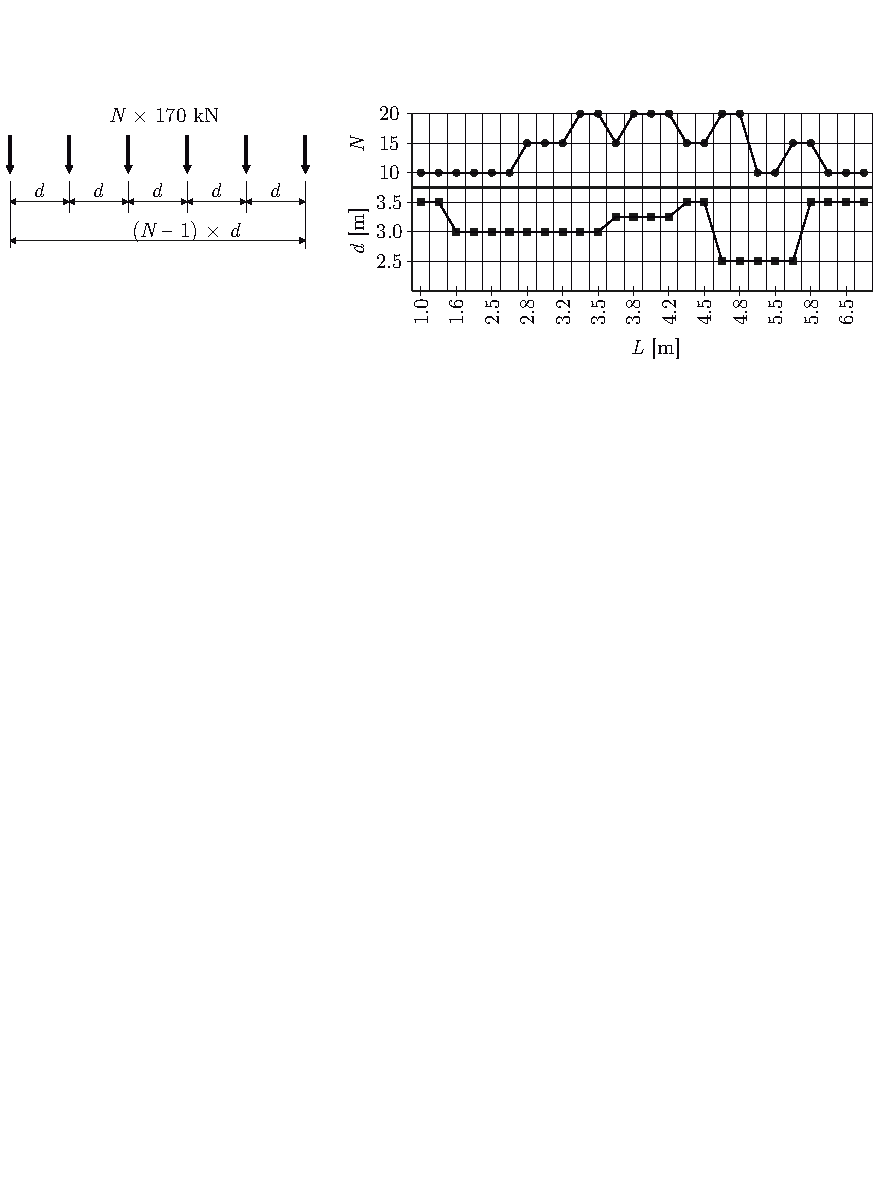
\includegraphics[]{/dynamic_railway/hslm_b.pdf}
	\captionsetup{justification=centering}
	\caption{Model pociagu HSLM-B według PN-EN 1991-2. Na podstawie \cite{PKNj}}
	\label{fig:train_hslm_b}
\end{figure}

\begin{table}[hbt!]
	\caption{Parametry modelu HSLM-A wg \cite{PKNj}}
	\centering
	\footnotesize
	\setlength\tabcolsep{0pt}
	\begin{tabular}{@{} P{0.1\textwidth} *4{P{0.225\textwidth}} @{}}
		\toprule
		HSLM & \begin{tabular}[c]{@{}c@{}}Liczba pośrednich\\ wagonów pasażerskich \\ $N$\end{tabular} & \begin{tabular}[c]{@{}c@{}}Długość wagonu\\ pasażerskiego \\ $D$ {[}m{]}\end{tabular} & \begin{tabular}[c]{@{}c@{}}Rozstaw osi\\ wózków \\ $d$ {[}m{]}\end{tabular} & \begin{tabular}[c]{@{}c@{}}Siła skupiona \\ $P$ {[}kN{]}\end{tabular} \\ \midrule
		A1   & 18                                                                                      & 18                                                                                    & 2.0                                                                         & 170                                                                   \\ %\midrule
		A2   & 17                                                                                      & 19                                                                                    & 3.5                                                                         & 200                                                                   \\ %\midrule
		A3   & 16                                                                                      & 20                                                                                    & 2.0                                                                         & 180                                                                   \\ %\midrule
		A4   & 15                                                                                      & 21                                                                                    & 3.0                                                                         & 190                                                                   \\ %\midrule
		A5   & 14                                                                                      & 22                                                                                    & 2.0                                                                         & 170                                                                   \\ %\midrule
		A6   & 13                                                                                      & 23                                                                                    & 2.0                                                                         & 180                                                                   \\ %\midrule
		A7   & 13                                                                                      & 24                                                                                    & 2.0                                                                         & 190                                                                   \\ %\midrule
		A8   & 12                                                                                      & 25                                                                                    & 2.5                                                                         & 190                                                                   \\ %\midrule
		A9   & 11                                                                                      & 26                                                                                    & 2.0                                                                         & 210                                                                   \\ %\midrule
		A10  & 11                                                                                      & 27                                                                                    & 2.0                                                                         & 210                                                                   \\ \bottomrule
	\end{tabular}
	\label{tab:hslm_a_parameters}
\end{table}

Drugą grupę obciążeń stosowanych w analizach dynamicznych stanowią pociągi uniwersalne \teng{Universal Trains}. W jej skład wchodzą dwa modele: HSLM-A i HSLM-B \teng{High Speed Load Model (HSLM)}. Są to modele teoretyczne, które powstały aby zagwarantować spełnienie warunków interoperacyjności kolei w państwach Unii Europejskiej. Odzwierciedlają szeroki zakres obciążeń wywołanych przez PDP obecnie użytkowane i potencjalnie występujące w przyszłości. 

Model obciążenia HSLM-A został przedstawiony na rysunku \ref{fig:train_hslm_a}, występuje w 10 wariantach oznaczonych od A1 do A10 i różniących się parametrami. Wartości zmiennych modelu HSLM-A przedstawiono w tabeli \ref{tab:hslm_a_parameters}. Schemat obciążenia stanowi potok sił, w większości rozstawionych w regularny sposób jak dla osi kół pociągu. Rozkład sił odpowiada pociągowi o typie przegubowym (rys. \ref{fig:train_types_EC_art}). Całkowita długość pociągu w każdym z wariantów wynosi około 400 m i zależy od liczby wagonów $N$ i ich długości $D$. Obciążenie przypadające na oś oznaczono jako $P$, a jego wartość mieści się w zakresie od 170 kN do 210 kN. Rozstaw osi wózków $d$ również został zróżnicowany od 2 do 3.5 m. Dodatkowo na początku i na końcu modelu znajduje się nieregularny układ sił odwzorowujący lokomotywy. 

Model HSLM-B pokazano na rysunku \ref{fig:train_hslm_b}. Składa się z $N$ sił w regularnym rozstawie $d$. Parametry modelu $d$ i $N$ przyjmuje się w zależności od rozpiętości przęsła $L$ zgodnie z nomogramem umieszczonym również na rysunku \ref{fig:train_hslm_b}. Zalecane jest by Model HSLM-B stosować dla obiektów 'prostych' o rozpiętości poniżej 7 m. Dla pozostałych konstrukcji zalecane jest wyznaczenie odpowiedzi od obciążenia modelem HSLM-A we wszystkich wariantach A1-A10.

\subsubsection{Parametry obciążenia ruchomego}

Analizując dynamicznie obiekty wzdłuż LDP należy zastosować modele obciążenia Pociągami Rzeczywistymi występującymi na linii oraz modele HSLM, jeśli dla linii stosowane są międzyoperacyjne kryteria europejskie dużych prędkości. Dla prędkości liniowej mniejszej niż 200 km/h, jeżeli analiza dynamiczna w ogóle jest wymagana, to do sprawdzenia efektów dynamicznych należy zastosować Pociągi Rzeczywiste A-F (załącznik F normy \cite{PKNj}) oraz Pociągi Zmęczeniowe 1-12 (załącznik D normy \cite{PKNj}).

Prędkości analizowanych przejazdów należy przyjmować od 40 km/h do maksymalnej prędkości obliczeniowej, z krokiem co 10 km/h. Maksymalną prędkość obliczeniową zaleca się przyjmować jako $1.2\,\times\,$\textit{maksymalna dopuszczalna prędkość pojazdu}. W pobliżu prędkości rezonansowych (\ref{eq:criticla_speed}) należy zagęścić dobór ujętych prędkości. Według przepisów \parencite{PKNj,UnionInternationaleDesCheminsDeFer2009} przyspieszenia powinny być wyznaczone w zakresie częstotliwości drgań do $f_{max}=\text{max}\{1.5n_0;n_3; 30\,\text{Hz}\}$, gdzie $n_0$ i $n_3$ oznaczają odpowiednio pierwszą i trzecią postać giętnych drgań własnych konstrukcji. W przypadku mostów zwykle decydujący jest warunek 30 Hz, ponieważ drgania o częstotliwości powyżej 20 Hz dotyczą zazwyczaj elementów drugorzędnych \parencite{Oleszek2015b}. Powyższy warunek ma również potwierdzenie w badaniach nad destabilizacją podsypki \parencite{Zacher2008}.

\subsubsection{Parametry mostów}
Na etapie projektowania istnieje szereg niepewności dotyczących konstrukcji. Odnoszą się one przede wszystkim do wymiarów elementów konstrukcji, ciężarów objętościowych materiałów, modułu sprężystości materiałów i tłumienia całej struktury. Wszystkie z tych czynników wpływają na masę, tłumienie i sztywność układu, co ma bezpośrednie przełożenie na częstotliwości drgań własnych i tłumienia modalne. W konsekwencji, decydują także o możliwości wystąpienia rezonansu i o amplitudach drgań. Najlepszym i najbardziej wiarygodnym źródłem parametrów przyjmowanych w analizach są wyniki eksperymentów na rzeczywistej konstrukcji. Naturalnie jest to możliwe ewentualnie w trakcie modernizacji lub naprawy obiekty, a nie przy projektowaniu. Z tego względu sformułowano następujące zalecenia.

Tolerancje wymiarów konstrukcji ograniczone są przez normy dotyczące danych materiałów (Eurokody od 2 do 4). Przy obliczeniach na etapie projektowania rekomendowane jest przyjmowanie wymiarów nominalnych.

Eurokody \cite{PKNg, PKNj} podają zalecenia dotyczące przyjmowania parametrów materiałowych kiedy nie ma możliwości wyznaczenia ich rzeczywistych (zmierzonych lub zidentyfikowanych) wartości. Według normy \cite{PKNj} w przypadku mostów kolejowych zalecane jest przyjmowanie masy konstrukcji i jej wyposażenia w dwóch wariantach. Dotyczy to głównie podsypki, która na kolejowych mostach stalowych stanowi bardzo istotną składową całkowitego ciężaru własnego. Ogólną regułą jest, że zwiększona masa powoduję obniżenie częstotliwości drgań własnych i zmniejszenie amplitud drgań. Stąd przy obliczeniu maksymalnych przyspieszeń należy przyjąć minimalną szacowaną wartość obciążenia podsypką. Z uwagi jednak na możliwość przeszacowania prędkości krytycznej (proporcjonalnej do częstotliwości drgań własnych) należy również sprawdzić przypadek górnego szacowania ciężaru własnego. Moduł sprężystości materiałów jest z reguły bardzo precyzyjnie określony w przypadku stali. Odwrotnie niż w przypadku masy, zwiększona sztywność powoduje zwiększenie częstotliwości drgań własnych. Z tego względu w przypadku zakładania sztywności elementów betonowych, połączeń czy posadowienia zalecane jest by przyjmować dolne szacowanie.

W dobie obliczeń za pomocą programów MES poprawne odwzorowanie sztywności oraz rozkładów masy (zwłaszcza w konstrukcjach stalowych) nie stanowi większego problemu. Jednakże do analizy dynamicznej należy określić jeszcze parametry tłumienia modalnego układu. Na etapie projektowania określa się je w sposób przybliżony na podstawie norm lub wartości zidentyfikowanych przez badania na podobnych, rzeczywistych konstrukcjach \parencite{Ladislav1996}. W normie \cite{PKNj} podano wartości, które są dolną, a zatem bezpieczną granicą oszacowania. Zalecane wartości przytoczono w tablicy \ref{tab:damping_code_eurocode}. 
\begin{table}[hbt!]
	\centering
	\footnotesize
	\setlength\tabcolsep{0pt}
	\caption{Zalecane wartości liczby tłumienia według normy \cite{PKNj}}
	\begin{tabular}{@{}p{0.4\textwidth} P{0.3\textwidth} P{0.3\textwidth} @{}}
		\toprule
		\multirow{2}{*}{Rodzaj mostu}    & \multicolumn{2}{c}{Dolna granica ułamka tłumienia {[}\%{]}} \\ \cmidrule(l){2-3} 
		& Rozpiętość $L<20$m         & Rozpiętość $L\ge 20$ m         \\ \midrule
		Stalowy i zespolony              & 0.5+0.125(20-L)            & 0.5                            \\ %\midrule
		Betonowy sprężony                & 1.0+0.07(20-L)             & 1.0                            \\ %\midrule
		Dźwigary obetonowane i żelbetowe & 1.5+0.07(20-L)             & 1.5                            \\ \bottomrule
	\end{tabular}
	\label{tab:damping_code_eurocode}
\end{table}
Z reguły w obliczeniach stosowane jest tłumienie proporcjonalne charakteryzujące się liniowym działaniem. Jest to również podejście bezpieczne, ponieważ uwzględnienie nieliniowego tłumienia skutkuje zmniejszeniem amplitud drgań \parencite{Ulker-Kaustell2012a,Oleszek2015}. 
Najczęściej spotykane normowe modele obciążenia wyrażone są za pomocą potoku sił, tworząc bezinercyjne schematy obciążenia. W konsekwencji przy tak wykonanej analizie nie uwzględnia się interakcji pomiędzy pojazdem, a konstrukcją. Z reguły uwzględnienie resorowania i tłumienia zawieszenia również zmniejsza amplitudy odpowiedzi układu w rezonansie. Ma to jednak istotne znaczenie głównie dla krótkich przęseł. W normie \cite{PKNj} efekt ten uwzględniono w sposób uproszczony przez zastosowanie nadwyżki tłumienia, dla obiektów o rozpiętości mniejszej niż 30 m. Całkowite tłumienie $\xi_{total}$ po uwzględnieniu nadwyżki wyrażone jest wzorem \ref{eq:total_damp_ec}, a dodatek tłumienia $\Delta \xi$ określony w funkcji rozpiętości przęsła $L$ zaproponowano w postaci równania \ref{eq:additional_damp_ec}.
\begin{equation} \label{eq:total_damp_ec}
	\xi_{total}=\xi + \Delta \xi
\end{equation}
\begin{equation} \label{eq:additional_damp_ec}
	\Delta \xi =\frac{0.0187L-0.00064L^2}{1-0.0441L-0.0044L^2+0.000255L^3}
\end{equation}








\subsubsection{Kryteria oceny rozwiązania} \label{sect: eurokod_kryteria_oceny}
Jeżeli analiza dynamiczna jest wymagana, norma PN-EN 1991-2 nakazuje wyznaczenie przemieszczeń i przyspieszeń przęsła oraz współczynnika $\phi'_{dyn}$ zdefiniowanego równaniem:
\begin{equation} \label{eq:phi_dyn}
	\phi '_{dyn} = \text{max}\Big| \frac{y_{dyn}}{y_{stat}} \Big| -1
\end{equation}
gdzie: $y_{dyn}$ oznacza maksymalną odpowiedź dynamiczną, a $y_{stat}$ odpowiadającą maksymalną odpowiedź statyczną od obciążenia Pociągiem Rzeczywistym lub modelem HSLM danego elementu konstrukcyjnego. Norma nie precyzuje jakie efekty należy porównywać przy wyznaczeniu współczynnika $phi '_{dyn}$, a bynajmniej nie jest to bez znaczenia dla wyniku. Przykładowo \cite{Klasztorny2005} wskazuje, że dla mostów belkowych stalowych i zespolonych współczynniki dynamiczne wyznaczane na podstawie ugięć są o około 10\% niższe niż dla naprężeń. W rozdziale 6.4.6.5 normy podano aspekty, które trzeba sprawdzić w celu zapewnienia bezpieczeństwa ruchu na obiekcie. Należą do nich sprawdzenie maksymalnych przyspieszeń przęsła w celu ochrony przed niestabilnością toru oraz uwzględnienie przyrostów dynamicznych obciążenia zarówno w nośności doraźnej, jak i zmęczeniowej.
Warunek ochrony przed niestabilnością toru omówiono w dalszej części rozdziału. Nośność doraźną należy określić przez sprawdzenie bardziej niekorzystnej z dwóch sytuacji:
\begin{itemize}
	\item efekty statyczne obciążenia modelem LM 71 powiększone przez odpowiadający mu współczynnik dynamiczny. Jeśli jest to wymagane, należy sprawdzić również obciążenie SW/0 ze współczynnikiem dynamicznym,
	\item efekty statyczne obciążenia Pociągiem Rzeczywistym (RT) lub HSLM, w obu przypadkach powiększone przez współczynnik dynamiczny $\phi '_{dyn}$ dany wzorem (\ref{eq:phi_dyn}) i współczynnik $\phi''$ wynikający z nierównomierności toru, zdefiniowany w załączniku C do PN-EN 1991-2.
\end{itemize}
Podsumowując powyższe, należy wyznaczyć efekty obciążenia zgodnie z poniższą formułą podaną w normie:
\begin{equation} \label{eq:SGN_dyna}
	\phi \times (LM\,71 \text{ \glqq +\grqq }\; SW/0)\quad \text{lub} \quad
	(1+\phi '_{dyn}+0.5 \times \phi'') \times 
	\begin{pmatrix}
		HSLM \\
		\text{lub} \\
		RT
	\end{pmatrix}
\end{equation}

Ważnym i obszernym zagadnieniem dotyczącym trwałości mostów kolejowych jest oszacowanie nośności zmęczeniowej. Norma nakazuje uwzględnienie przy badaniu wpływu zjawiska zmęczenia również efektów dynamicznych. Kiedy nie ma potrzeby wykonywania analiz dynamicznych, następuje to przez powiększenie obciążenia LM 71 o współczynnik dynamiczny. W przypadku prowadzenia analizy dynamicznej jej wyniki także powinny być uwzględnione przy ocenie nośności zmęczeniowej (p. 6.4.6.6 normy). Zjawisko zmęczenia oraz metody jego uwzględniania w mostach opisano w literaturze przedmiotu \parencite{Kocanda1985,Schijve2001,Malm2006,Siwowski2012,Siwowski2014,Szafranski2017}.


Norma PN-EN 1991-2 zwraca szczególną uwagę na sprawdzenie bezpieczeństwa nawierzchni kolejowej. W celu spełnienia wszystkich warunków bezpieczeństwa należy wyznaczyć i ocenić następujące wielkości:
\begin{itemize}
	\item przemieszczenia i przyspieszenia pionowe pomostu,
	\item skręcenie pomostu,
	\item przemieszczenia i przyspieszenia poziome pomostu.
\end{itemize}
Wszystkie kryteria opisano w PN-EN 1990 załącznik A2 w punkcie A2.4.4. Spośród powyższych decydujące jest zazwyczaj sprawdzenie przyspieszeń pionowych. Ze względu na ryzyko destabilizacji podsypki wyznaczone maksymalne pionowe przyspieszenia pomostu należy porównać z wartościami dopuszczalnymi podanymi w Eurokodzie 0 załącznik A.2. Wartości zalecane wynoszą odpowiednio $3.5\,\text{m/s}^2$ dla pomostu z nawierzchnią podsypkową oraz $5.0 \,\text{m/s}^2$ dla nawierzchni bezpodsypkowej. Wartości te wynikają wprost z wyników badań \parencite{Zacher2008} przy uwzględnieniu współczynników bezpieczeństwa. Dla nawierzchni z podsypką zastosowano współczynnik 2.0 i uzyskano $a_{dop}=7/2.0=3.5\,\text{m/s}^2$, a dla bezpodsypkowej 1.4 co prowadzi do wyniku $a_{dop}=7/1.4=5.0\,\text{m/s}^2$.
W przypadku mostów o dużych rozpiętościach decydujący może być również warunek narzucony na częstotliwość pierwszej, poziomej postaci drgań. \cite{PKNc} w regule opisuje, że najniższa częstotliwość poprzecznych drgań własnych mostu nie może być niższa niż 1.2 Hz. Warunek powstał na podstawie badań sześciu stalowych, łukowych bądź kratownicowych mostów kolejowych o pomoście otwartym i o zróżnicowanej rozpiętości od 31 do 119m \parencite{ERRI1996}. Jednakże w pracy \cite{Dias2008} autorzy na podstawie badań i analiz dynamicznych pod obciążeniem pionowym i poprzecznym dowiedli, że warunek ten nie powinien być stosowany bezrefleksyjnie i możliwe jest projektowanie obiektów o niższych częstotliwościach poprzecznych drgań własnych.

Trzecim kryterium, które należy sprawdzić dla obiektów kolejowych jest komfort pasażerów. W normie PN-EN 1990 przyjęto trzy klasy komfortu pasażerów: bardzo dobrą, dobrą i dostateczną. Przynależność do danej klasy komfortu zależy od maksymalnych wartości przyspieszeń działających na pasażera, a wiec mierzonych wewnątrz pojazdu. Wartości progowe przyspieszeń dla poszczególnych klas przytoczono w tablicy \ref{tab:comfort_classes}. 
\begin{table}[hbt!]
	\caption{Zalecane klasy komfortu według \parencite{PKNc}}
	\footnotesize
	\centering
	\begin{tabular}{@{}cc@{}}
		\toprule
		\multicolumn{1}{c}{Poziom komfortu} & \begin{tabular}[c]{@{}c@{}}Przyspieszenia pionowe\\ $b_v \;\text{[m/s}^2\text{]}$\end{tabular} \\ \midrule
		Bardzo dobry                        & 1.0                                                                                         \\ %\midrule
		Dobry                               & 1.3                                                                                         \\ %\midrule
		Dostateczny                         & 2.0                                                                                         \\  \bottomrule
	\end{tabular}
	\label{tab:comfort_classes}
\end{table}
Naturalnie w celu wyznaczenia przyspieszeń wewnątrz pojazdu w trakcie analiz dynamicznych należy posłużyć się modelem interakcji pomiędzy pojazdem, a mostem. Analiza dynamiczna w podstawowej formie jest zadaniem złożonym, a jej trudność jeszcze wzrasta przy włączeniu do współpracy pomostu i taboru. Z tego względu w normie znalazła się również uproszczona metoda oszacowania komfortu na podstawie pionowych przemieszczeń statycznych przęsła. Posiada ona jednak ograniczenia stosowania. Dotyczy ona jedynie przęseł o schemacie statycznym belki swobodnie podpartej lub belki ciągłej o niewielkim zróżnicowaniu rozpiętości i sztywności oraz o rozpiętościach mniejszych niż 120 m. Na wykresie \ref{fig:simpl_comfort_clas} przytoczono nomogram zawarty w normie. Przedstawiono na nim krzywe graniczne $L/\delta$ w funkcji prędkości przejazdu $V $ [km/h] i rozpiętości przęsła $L$ [m], dla konstrukcji w formie trzech przęseł swobodnie podpartych ustawionych jedno za drugim. Symbol $\delta$ oznacz przemieszczenia pionowe przęsła pod obciążeniem statycznym LM 71, z uwzględnieniem współczynnika dynamicznego i dla współczynnika klasy obciążenia $\alpha =1$. Jeżeli wyznaczony wskaźnik $L/\delta$ mieści się poniżej odpowiedniej krzywej i powyżej wartości 600 to zagwarantowany jest bardzo dobry komfort pasażerów. W normie podano szereg modyfikacji wartości podanych na wykresie, pozwalających ocenić spełnienie pozostałych klas komfortu, przypadki z inną liczbą przęseł swobodnie podpartych i dla belek ciągłych.

\begin{figure}[hbt!]
	\centering
	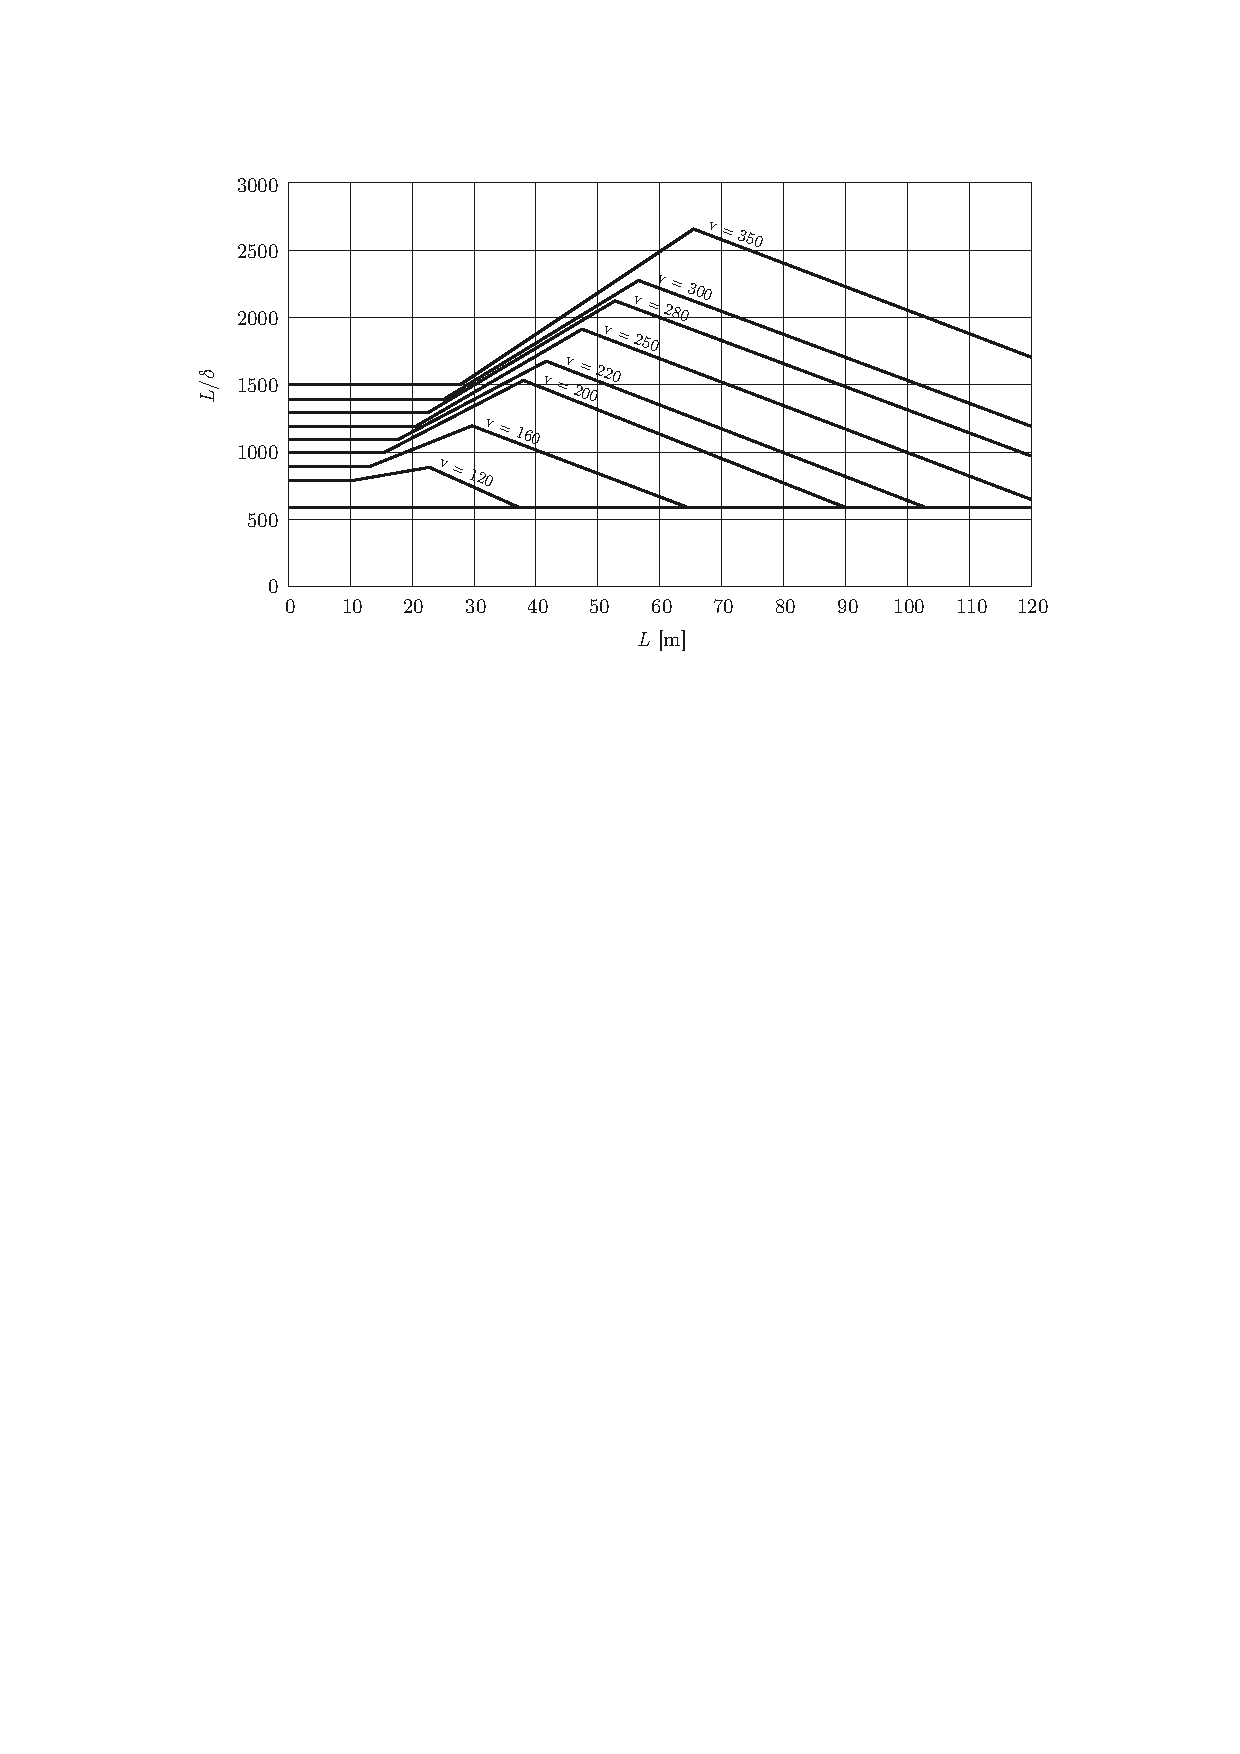
\includegraphics[]{/dynamic_railway/simp_comfort_class.pdf}
	\captionsetup{justification=centering}
	\caption{Nomogram do oceny komfortu w pojeździe na podstawie ugięć dla układu w postaci ciągu trzech przęseł swobodnie podpartych przy bardzo dobrym poziomie komfortu}
	\label{fig:simpl_comfort_clas}
\end{figure}

Dla sytuacjach niemieszczących się w obszarze stosowalności metody uproszczonej konieczne jest przeprowadzenie szczegółowej analizy dynamicznej. Norma wskazuje, że należy w niej uwzględnić:
\begin{itemize}
	\item szereg prędkości do wartości maksymalnej,
	\item obciążenie charakterystyczne pociagów rzeczywistych,
	\item dynamiczne współdziałanie mas między wagonami, a konstrukcją,
	\item charakterystyki modalne zawieszenia wagonu,
	\item liczbę wagonów wystarczającą do wywołania maksymalnych możliwych efektów,
	\item efekt działania nierównomierności toru na współdziałanie pojazdu z mostem.
\end{itemize}

Obiekt kolejowy uznaje się za poprawnie zaprojektowany jeśli spełnione są wszystkie Stany Graniczne Nośności i Użytkowania według PN-EN 1990 i PN-EN 1991-2, a zatem: warunki nośności doraźnej konstrukcji, trwałości zmęczeniowej, bezpieczeństwa nawierzchni kolejowej i odpowiedniego komfortu pasażerów.



	
%Dynamiczna Analiza Konstrukcji
\chapter{Analiza modalna i odpowiedź układów dynamicznych} \label{sect:modal_analysis_and_response}

\textit{Streszczenie: W niniejszym rozdziale przytoczono klasyfikację metod analizy modalnej oraz przewidywania odpowiedzi dynamicznej mostów. Zaprezentowano syntetyczny opis teoretycznej analizy modalnej oraz metody wyznaczania parametrów dynamicznych konstrukcji na bazie modelu numerycznego. W dalszej części scharakteryzowano metody analityczne i numeryczne wyznaczania odpowiedzi dynamicznej modelu o jednym i wielu stopniach swobody. Na końcu rozdziału omówiono metodę uwzględniania tłumienia w analizie konstrukcji.}

\vspace{1cm}
%\section{Wiadomości wstępne} \label{section: modalAnalysisIntro}


Podstawowym celem pracy jest określenie zależności pomiędzy przyjętymi rozwiązaniami konstrukcyjnymi łukowych mostów kolejowych, a ich zachowaniem dynamicznym, a także wybór rozwiązania najlepszego. Predykcja odpowiedzi, jak wspomniano wcześniej, możliwa jest dzięki analizie numerycznym modeli MES poddanych odpowiednim obciążeniom. Jednakże trzeba zdawać sobie sprawę z niepewności, które mogą wystąpić przy konstruowaniu założeń. Rodzaje niepewności omówiono w rozdziale (\ref{sect:calibration_model}). Powiedziano również, że jedną z metod eliminacji niektórych z nich jest kalibracja modelu numerycznego. Niemniej, aby model dostosować do działania rzeczywistej konstrukcji należy mieć punkt odniesienia. Potrzebna jest więc jakaś miara zachowania statycznego lub dynamicznego obiektu. W przypadku analizy statycznej takim odniesieniem mogą być pomiary statyczne ugięć, zarejestrowane na przykład w trakcie próbnego obciążenia. W przypadku analizy dynamicznej, do porównania będą służyć charakterystyki modalne: częstotliwości i postaci drgań własnych oraz tłumienia. Parametry te można zaczerpnąć z literatury na etapie projektowania. Na etapie badania rzeczywistej konstrukcji warto zidentyfikować je w sposób eksperymentalny. W poniższym rozdziale przytoczono podstawowe zagadnienia związane z analizą modalną i identyfikacją charakterystyk modalnych układu i  obliczeniami odpowiedzi dynamicznej. Metody te zostaną w dalszej części pracy zastosowane w obliczeniach numerycznych i optymalizacyjnych.

\section{Analiza modalna} \label{section: modalAnalysisIntro}
W odpowiedzi na zapotrzebowanie przewidywania i kontroli drgań konstrukcji, w sposób naturalny rozwinęła się dziedzina nauki zajmująca się opisem i modelowaniem zjawisk dynamicznych. Podstawowym narzędziem służącym identyfikacji parametrów modalnych i testowaniu zachowania dynamicznego struktury jest analiza modalna \teng{modal analysis}. W najogólniejszym sensie analiza modalna służy określeniu częstotliwości drgań własnych oraz odpowiadających postaci i tłumień. Często analiza modalna bywa określana jako identyfikacja modalna \teng{modal identification}, a pojęcia te są traktowane zamiennie. Bywa, że niektórzy badawcze ograniczają znaczenie pojęcia analizy modalnej jedynie do wybranych metod jakie wchodzą w skład tego szerokiego pojęcia. W niniejszej pracy analizą modalną nazwane są wszystkie techniki służące poszukiwaniu parametrów modalnych konstrukcji.

W pracy \parencite{Zhang2004} autor definiuje identyfikację modalną jako gałąź szerszego pojęcia identyfikacji systemów, a jej celem jest budowa modelu matematycznego systemu dynamicznego poprzez pomiar i analizę zestawu danych wejściowych i wyjściowych. Modelem matematycznym w zagadnień dynamiki budowli jest zazwyczaj równanie lub zbiór równań, które opisują ruch modelu mechanicznego. Aby metody analizy modalnej miały zastosowanie, model matematyczny musi spełniać następujące założenia \parencite{Maia1997}:
\begin{itemize}
	\item system jest liniowy,
	\item parametry systemu są niezależne od czasu,
	\item system jest obserwowalny,
	\item obowiązuje zasada wzajemności Maxwell'a.
\end{itemize}

Ewins w  pracy \cite{Ewins2000} podaje trzy główne powody przeprowadzania analizy modalnej:
\begin{itemize}
	\item ocena źródła drgań i ich przebiegu,
	\item weryfikacja modeli teoretycznych i przewidywanie zjawisk dynamicznych,
	\item identyfikacja charakterystyk materiałowych ciała poddanego wymuszeniu dynamicznemu (np. tłumienie, tarcie, wytrzymałość zmęczeniowa). 
\end{itemize}
Każdy z powyższych celów może być jedynie środkiem do osiągnięcia zupełnie innego. W rzeczywistości tak właśnie jest najczęściej, o czym świadczy mnogość aplikacji analizy modalnej w bardzo różnych zagadnieniach dotyczących konstrukcji. 


\subsection{Klasyfikacja metod analizy modalnej}

Identyfikacja modalna jest zbiorem technik, które są rozwijane dynamicznie od lat 60' XX w. Gwałtowny przyrost zainteresowania tym tematem wywołał głównie rozwój technik cyfrowych \parencite{Ewins2000}. Do tej pory powstało wiele różnych technik, których krótką klasyfikację z podziałem na główne kryteria podano w tym podrozdziale.

Matematyczne modele modalne mogą charakteryzować się różnym stopniem skomplikowania. Jak już wspomniano, parametrami które mogą opisywać model są postaci drgań własnych oraz powiązane z nimi częstotliwości i tłumienia modalne, a także masa i sztywność modalna. Metody analizy modalnej różnią się chociażby tym, które z tych informacji mogą dostarczyć. Z tego względu wybór odpowiedniej metody powinien być świadomy i poparty przeglądem wielu technik, z których wybrana zostanie ta odpowiadająca potrzebom. Aspektami mogącymi wpłynąć na wybór metody są między innymi: czas potrzebny do implementacji (pierwszego użycia), informacje możliwe do uzyskania z modelu, możliwy wpływ założeń i uproszczeń, liczba parametrów potrzebnych do stworzenia modelu czy też stabilność rozwiązania. Podstawowe pozycje literaturowe, w których zawarto dokładny opis metod ze wskazówkami do ich użycia to \parencite{Ewins2000,Maia1997,Zhang2004,Brincker2015,Rainieri2014}. Poniżej dokonano jedynie klasyfikacji i omówienia podstawowych kryteriów podziału.

Najogólniej analizę modalną można podzielić na dwie główne gałęzie zależne od typu stosowanej procedury ogólnej, zależnej od rodzaju danych wejściowych i oczekiwanych rezultatów. Te dwie obszerne grupy nazywa się teoretyczną i eksperymentalną analizą modalną \parencite{Lengvarsky2013}. W niniejszej pracy wielokrotnie używane będą oba podejścia, dlatego autor zdecydował się na krótki ich opis. Ogólny schemat procedur teoretycznej i doświadczalnej analizy modalnej pokazano na rysunku \ref{fig:theExpProc}.  

\begin{figure}[hbt!]
	\centering
	\subfloat[Procedura teoretyczna]{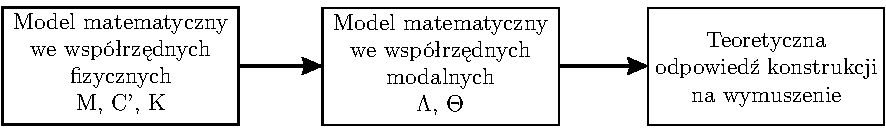
\includegraphics[width=\textwidth]{/modal_analysis/schemat_theory_exper_a.pdf}
		\label{fig:theExpProcA}
	} \\
	\subfloat[Procedura doświadczalna]{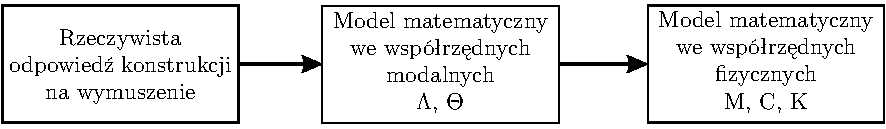
\includegraphics[width=\textwidth]{/modal_analysis/schemat_theory_exper_b.pdf}
		\label{fig:theExpProcB}}
	\captionsetup{justification=centering}
	\caption{Porównanie procedur teoretycznej i doświadczalnej analizy modalnej}
	\label{fig:theExpProc}
\end{figure}

Metody teoretyczne opierają się na rozwiązaniach analitycznych lub numerycznych (rys. \ref{fig:theExpProcA}). Badanie zachowania dynamicznego rozpoczyna się od definicji struktury, najczęściej za pomocą modelu dyskretnego opisanego macierzami $\mathbf{M}, \mathbf{C}', \mathbf{K}$, oznaczającymi odpowiednio macierz mas, tłumienia i sztywności. Na etapie dzisiejszej wiedzy, w przypadku metod teoretycznych macierz tłumienia przyjmowana jest na podstawie doświadczeń lub badań eksperymentalnych i stąd została oznaczona apostrofem $\mathbf{C'}$. Za pomocą przekształceń matematycznych tworzony jest model matematyczny we współrzędnych modalnych. Uzyskiwane są charakterystyki modalne układu $\mathbf{\Lambda}$ i $\mathbf{\Phi}$, odpowiednio częstości drgań własnych, postaci drgań własnych i dodatkowo parametry opisujące przyjęty model tłumienia. Metody analityczne znajdują realne zastosowanie w przypadku obiektów, których opis ciągły nie jest złożony, a dyskretny ograniczony jedynie do niewielkiej liczby stopni swobody. Rzeczywiste konstrukcje są układami o nieskończonej liczbie stopni swobody. Niemniej, sprowadzenie ich do skończonej (choć zazwyczaj bardzo dużej) liczby stopni swobody pozwala otrzymać zadowalająco dokładne rezultaty. W przypadku dużej liczby stopni swobody najszerzej stosowane są metody przybliżone opierające się obliczeniach numerycznych. Teoretyczna analiza modalna ma wiele zalet. Pozwala uzyskać parametry modalne relatywnie szybko i tanio. Wynika to z powszechności narzędzi do modelowania i obliczania konstrukcji. W obrębie modelowania realnych struktur współczesne oprogramowanie pozwala budować modele numeryczne praktycznie bez ograniczeń. Pomimo wielu niewątpliwych zalet, teoretyczna analiza modalna posiada ograniczenia, z których należy zdawać sobie sprawę. Przede wszystkim jakość rezultatów zależy wprost od jakości wprowadzonych przez użytkownika danych. W przypadku zagadnień dynamicznych kolejnym bardzo ważnym ograniczeniem jest brak analitycznej możliwości określenia tłumienia konstrukcji. Taką możliwość daje jedynie badanie doświadczalne. Metody analityczne i numeryczne są obszernie opisane w wielu publikacjach \parencite{Chmielewski1998,Chopra2012a,Rucka2014}. W dalszej części rozdziału zaprezentowano absolutne podstawy i założenia teoretycznej analizy modalnej.


%\cite{Brincker2015} wskazuje na następujące źródła błędów i szacowane poziomy niepewności rezultatów analizy w zależności od rodzaju popełnionego błędów w definicji modelu MES (tab):

Doświadczalna analiza w odróżnieniu od wersji teoretycznej angażuje do identyfikacji warsztat badawczy. Jak przedstawiono na rysunku (rys. \ref{fig:theExpProcB}) ten typ analizy ma niejako odwrotny kierunek niż teoretyczna analiza modalna. W tym przypadku odpowiedź konstrukcji jest mierzona i na jej podstawie wyznaczane są wielkości opisujące model matematyczny: $\mathbf{\Lambda}$ i $\mathbf{\Phi}$. Następnie dopiero na ich podstawie możliwe jest przekształcenie na model matematyczny wyrażony we współrzędnych fizycznych: $\mathbf{M}, \mathbf{C}, \mathbf{K}$. Doświadczalna analiza modalna dzieli się na dwie główne odnogi związane z zakresem rejestrowanych danych w trakcie wykonywania eksperymentu. Pierwsza z nich to Eksperymentalna Analiza Modalna (EMA) \teng{Experimental Modal Analysis}, która wymaga pomiaru sił wymuszających oraz odpowiedzi konstrukcji na to wymuszenie. Druga to Operacyjna Analiza Modalna (OMA) \teng{Operational Modal Analysis}, która estymuje parametry modalne wyłącznie na podstawie pomierzonych efektów nieznanego wymuszenia. 

Kwestia pomiaru sił wymuszających wpływa na podstawowe różnice pomiędzy EMA i OMA \cite{Bien2007}. EMA najczęściej prowadzona jest w kontrolowanych warunkach i przez to z reguły pozwala uzyskać dokładniejsze informacje na temat zachowania dynamicznego konstrukcji. Jednakże w przypadku rzeczywistych budowli trudno jest stworzyć takie kontrolowane warunki. W przypadku mostów, obiekt musiałby na czas badań zostać wyłączony z eksploatacji. Okazuje się to często niemożliwe z przyczyn proceduralnych, a do tego zawsze jest kosztowne. Drugim zasadniczym zagrożeniem powodzenia eksperymentu EMA jest potrzeba stworzenia takiego systemu wymuszenia, które wywoła mierzalną odpowiedź konstrukcji. W przypadku dużych konstrukcji inżynierskich może okazać się to trudne do zrealizowania. Oddziaływania środowiskowe często wywołują efekty porównywalne z kontrolowanym wymuszeniem. Z kolei w OMA badania prowadzone mogą być przy normalnej eksploatacji, a losowe oddziaływania środowiskowe zazwyczaj tylko polepszają jakość wyników. Niemniej jednak, teoretyczne założenia OMA prawie zawsze są spełnione jedynie w sposób przybliżony. Wpływa to na zwiększenie wymaganej długości prowadzenia pomiarów, a interpretacja wyników wymaga większego doświadczenia. 

W dalszej części tego rozdziału opisano najważniejsze - według autora - pojęcia, których zrozumienie było kluczowe do wyznaczania parametrów modalnych modelu numerycznego i odpowiedzi dynamicznej konstrukcji. Do identyfikacji modalnej istniejącej konstrukcji wykorzystano Operacyjną Analizę Modalną. Rodzinę metod OMA wraz z zastosowaniem i aplikacją przedstawiono w rozdziale \ref{sect:OMA}.

\section{Teoretyczna analiza modalna}
\label{section: eigen}
Metody teoretycznej analizy modalnej rzeczywistych konstrukcji w praktyce mają zastosowanie głównie w formie rozwiązań numerycznych prowadzonych na modelach MES. Poniżej (\ref{eq: mot_dam}) przedstawiono macierzowe równanie równowagi sił w dynamice dla tłumionego układu o skończonej liczbie stopni swobody.
\begin{equation} \label{eq: mot_dam}
\vect{M} \vect{\ddot{x}}(t) +\vect{C} \vect{\dot{x}}(t)+ \vect{Kx}(t) = \vect{F}(t)
\end{equation}
gdzie $\vect{M},\vect{C},\vect{K}$ to odpowiednio macierze mass, tłumienia i sztywności, $\vect{x}$ to wektor współrzędnych uogólnionych (przemieszczeń lub obrotów), $\vect{F}(t)$ to wektor uogólnionych sił wymuszających. Pozbawiając wzór (\ref{eq: mot_dam}) czynnika odpowiadającego za tłumienie, otrzymamy formułę (\ref{eq: mot_und}) opisującą ruch nietłumiony wymuszonego układu dynamicznego. 
\begin{equation} \label{eq: mot_und}
\vect{M} \vect{\ddot{x}}(t) +\vect{Kx}(t) = \vect{F}(t)
\end{equation}

Drgania swobodne są procesem fizycznym spowodowanym zaburzeniem stanu równowagi statycznej, przez zaistnienie niezerowych warunków początkowych. Macierzowe równanie ruchu drgań swobodnych, tłumionych opisane jest wzorem (\ref{eq: mot_dam_free}), a nietłumionych wzorem (\ref{eq: mot_und_free}). Równania te nie zawierają składnika sił wymuszających.
\begin{equation} \label{eq: mot_dam_free}
\vect{M} \vect{\ddot{x}}(t) +\vect{C} \vect{\dot{x}}(t)+ \vect{Kx}(t) = \vect{0}
\end{equation}

\begin{equation} \label{eq: mot_und_free}
\vect{M} \vect{\ddot{x}}(t) +\vect{Kx}(t) = \vect{0}
\end{equation}

Okazuje się, że parametry modalne systemu są ściśle powiązane z rozwiązaniem algebraicznego problemu własnego równań drgań swobodnych. 

\subsection{Zagadnienie własne} \label{sect:modal_analysis}
Identyfikacja modalna modelu numerycznego, polegająca na wyznaczeniu częstotliwości i postaci drgań własnych, sprowadza się do rozwiązania zagadnienia własnego. Bardzo pozytywnym aspektem tej zależności jest to, że istnieje wiele prostych w aplikacji, wydajnych i dokładnych algorytmów pozwalających rozwiązać numerycznie zagadnienie własne \parencite{Golub2013}. Dzięki temu, właśnie ta metoda identyfikacji modalnej cieszy się największą popularnością wśród producentów oprogramowania do obliczania konstrukcji. Użytkownicy oprogramowania mogą bez większego wysiłku dokonać identyfikacji parametrów modalnych nawet złożonych modeli numerycznych. Poniżej zaprezentowano zasady formułowania i właściwości zagadnienia własnego dla układu bez tłumienia (\ref{eq: mot_und_free}) i układu z tłumieniem (\ref{eq: mot_dam_free})
\subsubsection{Układ nietłumiony}
Z reguły przyjmuje się, że rozwiązanie zagadnienia własnego wykorzystuje równanie drgań swobodnych nietłumionych (\ref{eq: mot_und_free}). Należy zaznaczyć, że drgania własne nie opisują procesu fizycznego, a są jedynie matematyczną idealizacją drgań układu. W przypadku drgań własnych nietłumionym, dla każdego z modów układ oscyluje wokół położenia równowagi statycznej z częstotliwością drgań własnych, a wszystkie stopnie swobody drgają w tej samej fazie. Oznacza to, że każdy z punktów osiąga swoje ekstremalne położenie w tej samej chwili. Podobnie wszystkie punkty znajdują się w położeniu równowagi statycznej w tym samym czasie. Poniżej przedstawiono rozwiązanie zagadnienia własnego dla nietłumionego układu $N$ dynamicznych stopni swobody.

Złóżmy, że rozwiązanie równania (\ref{eq: mot_und_free}) ma postać $\vect{x}(t)=\vect{\phi}e^{j\omega t}$ gdzie $\omega$ to częstość drgań własnych, $j=\sqrt{-1}$, a $\phi$ to niezerowy wektor postaci drgań własnych. Po podstawieniu rozwiązania i jego drugiej pochodnej ($\vect{\ddot{x}}(t)=-\vect{\phi} \omega^2 e^{j\omega t}$) do równia (\ref{eq: mot_und_free}) otrzymamy równanie (\ref{eq: char_equation1}).

\begin{equation} \label{eq: char_equation1}
-\vect{M}\vect{\phi}\omega^2 e^{j\omega t} +\vect{K\phi}e^{j\omega t} = \vect{0}
\end{equation}
Dzieląc strony równania przez niezerową wartość $e^{j\omega t}$ otrzymujemy układ liniowych równań algebraicznych:
\begin{equation} \label{eq: char_equation2}
-\vect{M}\omega^2 \vect{\phi} +\vect{K\phi} = \vect{0}
\end{equation}
w którym dwie niewiadome do ustalenia to: $\phi$ - niezerowy wektor postaci drgań własnych oraz $\omega$ - częstość drgań własnych. Równanie to można zapisać w formie (\ref{eq: char_equation3}) z indeksami określającymi poszczególne mody drgań własnych. Liczba par odpowiadających sobie częstości $\omega_i$ i postaci drgań własnych $\phi_i$ jest równa liczbie $N$ stopni swobody. 
\begin{equation} \label{eq: char_equation3}
\omega^2_i \vect{M}\phi_i = \vect{K}\phi_i\qquad i=1,2,...,N
\end{equation}
Z kolei równanie (\ref{eq: char_equation4}) to reprezentacja uogólnionego problemu własnego, w którym $\lambda_i$ to wartość własna, a $u_i$ to wektor własny.  
\begin{equation} \label{eq: char_equation4}
\lambda_i \vect{A}u_i = \vect{B}u_i
\end{equation}
Z porównania wzorów (\ref{eq: char_equation3}) i (\ref{eq: char_equation4}) wyraźnie widać analogię $\lambda_i=\omega^2_i$. Wynika z tego, że rozwiązanie numeryczne uogólnionego problemu własnego pozwala wprost uzyskać częstości $(\lambda_i=\omega^2_i)$ i postaci drgań własnych $(u_i=\phi_i)$.

Układ równań (\ref{eq: char_equation3}) ma nietrywialne rozwiązania tylko, jeśli spełniona jest zależność:
\begin{equation} \label{eq: char_equation_det}
\det[\vect{K}-\omega^2_i \vect{M}] = \vect{0}
\end{equation}
Formuła (\ref{eq: char_equation_det}) jest znana jako równanie charakterystyczne zagadnienia własnego. Rozwijając wyznacznik, otrzymamy wielomian stopnia $N$ względem $\omega^2_i$. Pierwiastkami równania (\ref{eq: char_equation_det}) są częstości drgań własnych $\omega_i$. Znając częstości własne $\omega_i$, z równania (\ref{eq: char_equation3}) można obliczyć odpowiadające wektory własne $\phi_i$ z dokładnością do stałego czynnika. Taki wynik bywa nieprzystępny w ocenie więc wektory poddawane mogą być normalizacji. Do najczęściej stosowanych metod normalizacji należy taka modyfikacja wektora, aby maksymalna wartość bezwzględna spośród wszystkich współrzędnych wektora była równa jedności. Innym przykładem może być normalizacja wektorów tak, aby wartość elementu dla danego stopnia swobody, we wszystkich wektorach była równa jedności.

Jeżeli macierze $\vect{M}$ i $\vect{K}$ ($\vect{A}$ i $\vect{B}$ wg (\ref{eq: char_equation4})) są symetryczne i dodatnio określone o wartościach rzeczywistych to wartości oraz wektory własne są również rzeczywiste. W przypadku konstrukcji budowlanych macierz $\vect{K}$ jest zawsze dodatnio określona ponieważ warunki brzegowe zapewniają brak ruchu ciała jako bryły sztywnej. Nie jest to oczywiste dla innych niż struktur, takich jak na przykład samolot w locie \parencite{Chopra2012a}.


Postaci drgań własnych (wektory własne) odpowiadające różnym częstościom własnym spełniają warunki ortogonalności. W przypadku gdy $\omega_i \neq \omega_j$ prawdziwe są zależności (\ref{eq: eigenvect_orto}). Ortogonalność wektorów własnych może być wykorzystana do weryfikacji obliczonych wektorów. 
\begin{equation} \label{eq: eigenvect_orto}
\vect{\phi}_i^{T}\vect{K\phi}_j = 0 \qquad \vect{\phi}_i^{T}\vect{M\phi}_j = 0
\end{equation}

Obliczone z równania \ref{eq: char_equation_det} wartości oraz wektory własne możemy przedstawić w postaci dwóch specjalnych macierzy. $N$ obliczonych wartości własnych zestawionych w macierz diagonalną tworzy tak zwaną macierz widmową (\ref{eq: mat_spect}). Z kolei $N$ wektorów własnych zestawionych kolumnowo nazywamy macierzą modalną (\ref{eq: mat_modal}).

\begin{equation}  \label{eq: mat_spect}
\vect{\Omega}^2 =  
\begin{bmatrix} 
	\omega_{1}^2 & 0 			& \dots  & 0      \\ 
	0 		     & \omega_{2}^2 & \dots  & 0      \\
	\vdots       & \vdots       & \ddots & \vdots \\
	0 			 & 0 		    & \dots  & \omega_{N}^2 


\end{bmatrix}
\end{equation}

\begin{equation} \label{eq: mat_modal}
	\vect{\phi} = [\phi_{i,j}]= 
	\begin{bmatrix} 
		\phi_{11} & \phi_{12} & \dots & \phi_{1N} \\ 
		\phi_{12} & \phi_{22} & \dots & \phi_{2N} \\
		\vdots    & \vdots    & \ddots & \vdots \\
		\phi_{N1} & \phi_{N2} & \dots & \phi_{NN} 
	
	
	\end{bmatrix}
	\qquad
	1\leq i,j \leq N.
\end{equation}

Dla układu o $N$ stopniach swobody możemy wyznaczyć $N$ par częstotliwości i postaci drgań własnych. Jednak w rzeczywistości rozwiązanie ogranicza się do wyznaczenia jedynie ograniczonej do kilkunastu (maksymalnie kilkuset) pierwszych par. Określenie \enquote{pierwszych} właściwe jest w przypadku kiedy wyznaczone częstości uporządkujemy w szeregu rosnącym:
\begin{equation} \label{eq: eigenvalues_list}
0 \leq \omega_1  \leq \omega_2 \dots  \omega_{N-1} \leq  \omega_N
\end{equation}

W większości przypadków zagadnienie własne jest rozwiązywane numerycznie za pomocą komputerów. Metody numeryczne wykorzystują iteracyjne algorytmy do rozwiązania zagadnienia własnego. Chopra  definiuje trzy główne kategorie algorytmów \cite{Chopra2012a}: 
\begin{itemize}
	\item metody iteracji wektora wykorzystujące właściwości równania (\ref{eq: char_equation3}),
	\item metody transformacyjne korzystające z ortogonalności wektorów własnych,
	\item metody iteracyjne wykorzystujące równanie charakterystyczne (\ref{eq: char_equation_det}).
\end{itemize}
Dla dużych systemów korzystne okazuje się łączenie algorytmów z tej samej bądź różnych kategorii, co podnosi wydajność metody rozwiązania. W oprogramowaniu komercyjnym stosowane są złożone algorytmy takie jak metoda iteracji podprzestrzeni, metoda Lanczosa czy metoda gradientów Ritza. Wybór metody zależy również od wybranego solvera (silnika programu rozwiązującego równania). Algorytmy te różnią się pod względem wydajności, maksymalnej dokładności rozwiązania czy zbieżności. Ich wydajność może zależeć od liczby zadanych do wyznaczenia wartości własnych czy wielkości zadania. Więcej szczegółów odnośnie stosowanych metod rozwiązania zagadnienia własnego można odnaleźć w literaturze \parencite{Bathe2006,Wilson1983,Wilson1997,Fialko2000,Papadrakakis1993,Hughes1987,Chopra2012a}. W przypadku dobrej jakości oprogramowania komercyjnego informacje na temat używanych algorytmów powinny dostępne w dokumentacji programu.

\subsubsection{Układ tłumiony}
Drgania swobodne tłumione układu MDOF określone są równaniem (\ref{eq: mot_dam_free}), które przywołano dla wygody poniżej:
\begin{equation} \label{eq: mot_dam_free2}
\vect{M} \vect{\ddot{x}}(t) +\vect{C} \vect{\dot{x}}(t)+ \vect{Kx}(t) = \vect{0}
\end{equation}
Rozwiązanie tego równania jest uzależnione od postaci tłumienia. Może być ono klasyczne lub nieklasyczne. Tłumienie klasyczne zwane również proporcjonalnym \teng{classical damping, proportional damping} występuje w przypadku kiedy spełnione jest równanie (\ref{eq: class_damp}). 
\begin{equation} \label{eq: class_damp}
\vect{CM}^{-1}\vect{K} = \vect{KM}^{-1}\vect{C}
\end{equation}
Kiedy macierz $\vect{C}$ jest diagonalna to warunek (\ref{eq: class_damp}) jest spełniony. W takim przypadku wszystkie częstości drgań własnych są rzeczywiste i identyczne do tych wyznaczonych dla układu nietłumionego. W przypadku przeciwnym mamy do czynienia z tłumieniem nieklasycznym bądź nieproporcjonalnym \teng{nonclassical damping, nonproportional damping}. Dla tej sytuacji macierz $\vect{C}$ nie jest diagonalna, a wartości własne są zespolone. Szczegółowe informacje oraz metody rozwiązania przypadków dynamiki konstrukcji nieklasycznie tłumionych podano w \parencite{Caughey1961,Chopra2012a}. W pracy \cite{Inman1995} autorzy pokazali na przykładzie, że obliczanie struktur charakteryzujących się tłumieniem nieklasycznym za pomocą zagadnienia własnego, bez uwzględnienia macierzy tłumienia możne prowadzić do błędnych rezultatów. Tak wyznaczone częstotliwości drgań będą różnić się od rzeczywistych, co może pociągnąć za sobą błędne wnioski odnośnie zakresu częstotliwości grożących rezonansem.
\subsection{Transformacja do współrzędnych normalnych} \label{section: transform_normal}
Rozważmy ponownie równanie ruchu układu MDOF (\ref{eq: mot_dam_free2}). Wiemy, że każdy wektor o długości $N$ może być przedstawiony jako kombinacja liniowa $N$ liniowo niezależnych wektorów. Przedstawmy zatem wektor przemieszczeń $\vect{x}$ jako kombinację wektorów własnych: $\vect{\phi}$.
\begin{equation} \label{eq: normal_coord_komb}
	\vect{x} = \sum_{r=1}^{N} \vect{\phi}_r q_r=\vect{\phi q}
\end{equation} 
gdzie współczynniki $q_r$ nazywane są współrzędnymi normalnymi \teng{modal coordinates, normal coordinates} i $\vect{q}=<q_1\,\,q_2\,\, \dots\,\, q_N>^T$. Załóżmy, że zagadnienie własne zostało rozstrzygnięte i wyznaczyliśmy macierz modalną $\vect{\phi}$ (\ref{eq: mat_modal}). Aby uzyskać wartości współczynników $q_n$ dla danego $\vect{x}$, przemnóżmy obie strony równania (\ref{eq: normal_coord_komb}) przez $\vect{\phi}_n^T\vect{M}$:
\begin{equation} \label{eq: normal_coord_komb2}
	\vect{\phi}_n^T\vect{M}\vect{x} = \sum_{r=1}^{N} (\vect{\phi}_n^T\vect{M}\vect{\phi}_r) q_r
\end{equation} 

Ortogonalność wektorów własnych (\ref{eq: eigenvect_orto}) sprawia, że wszystkie składniki powyższej sumy są równe 0 poza tymi, w których $r=n$. Pomińmy więc znak sumy i zapiszmy 
\begin{equation} \label{eq: normal_coord_kom3}
	\vect{\phi}_n^T\vect{M}\vect{x} = (\vect{\phi}_n^T\vect{M}\vect{\phi}_n) q_n
\end{equation} 

\begin{equation} \label{eq: normal_coord_kom4}
	q_n = \frac{\vect{\phi}_n^T\vect{M}\vect{x}}{\vect{\phi}_n^T\vect{M}\vect{\phi}_n} 
\end{equation} 
Transformacja do współrzędnych normalnych zostanie wykorzystana przy przewidywaniu odpowiedzi wymuszonych, liniowych układów MDOF z tłumieniem proporcjonalnym (p. \ref{section: mdof_response}).

%Należy wspomnieć, że uogólniony problem własny nie jest jedyną metodą rozwiązania macierzowego równania ruchu. Przy spełnieniu powyższych warunków możliwe jest również przekształcenie uogólnionego problemu własnego w odpowiedni standardowy (prosty) problem własny:
%\begin{equation} \label{eq: eige_stan_1}
%\vect{A}u_i = \lambda_i u_i
%\end{equation}
%Aby doprowadzić równanie \ref{eq: char_equation3} do postaci standardowego problemu własnego wymagane jest wyznaczenie macierzy odwrotnej $\vect{M}^{-1}$. W przypadku kiedy jest to możliwe (na przykład przy pomocy dekompozycji Choleskiego) należy pomnożyć lewostronnie strony równania przez $\vect{M}^{-1}$ co pozwala uzyskać postać (\ref{eq: eige_stan_2}). Ponownie widoczne jest podobieństwo pomiędzy równaniami i powiązanie $(\lambda_i=\omega^2_i)$. Sprowadzenie do standardowego problemu własnego bywa korzystne z punktu widzenia rozwiązania numerycznego. 
%\begin{equation} \label{eq: eige_stan_2}
%\vect{M}^{-1}\vect{K}\phi_i=\omega^2_i\phi_i
%\end{equation}
\section{Metody wyznaczania odpowiedzi dynamicznej konstrukcji} \label{sect:dynamic_response_methods}
Wykorzystując przedstawiony w tym rozdziale opis matematyczny ruchu drgającego układów dyskretnych, poniżej zawarto metody przewidywania odpowiedzi tychże układów. W rozdziale dotyczącym efektów dynamicznych w mostach kolejowych (p. \ref{sect:railway_dynamic_effects}) wspomniano o rozwoju metod wyznaczania odpowiedzi dynamicznej pod obciążeniem ruchomym. Poniżej przywołano charakterystykę niektórych z nich. Szczególną uwagę zwrócono na metodę Newmarka, która została wielokrotnie wykorzystana w pracy. Przegląd metod pozwalających wyznaczyć odpowiedź konstrukcji poddanej wymuszeniu wypada zacząć klasycznie od układu z jednym stopniem swobody. 



\subsection{Odpowiedź systemów dynamicznych o jednym stopniu swobody} \label{section: sdof_response}

W przypadku liniowego układu SDOF obciążonego siłą zewnętrzną, równanie ruchu jest liniowym równaniem różniczkowym drugiego rzędu (\ref{eq: eq_mot_sdof}). Znając warunki początkowe $x(0)$ i $\dot{x}(0)$ możemy traktować zadanie jako w pełni sformułowane. Dla konstrukcji wstępnie nieobciążonej dynamicznie przemieszczenie i prędkość początkowe można przyjąć jako równe zeru.
\begin{equation} \label{eq: eq_mot_sdof}
	m\ddot{x}+c\dot{x}+k{x}=f(t)
\end{equation}
Dla tak sformułowanego problemu istnieją cztery podstawowe metody wyznaczenia odpowiedzi dynamicznej:
\begin{itemize}[noitemsep]
	\item klasyczne rozwiązanie równań różniczkowych,
	\item wykorzystanie całki Duhamela,
	\item rozwiązanie w dziedzinie częstotliwości,
	\item wykorzystanie metod numerycznych.
\end{itemize}
Dla porządku powyższe metody zostaną w dalszej części krótko opisane. Dokładny opis metod jest przedstawiony w podstawowych pozycjach literaturowych dotyczących dynamiki budowli \parencite{Clough1975,Chmielewski1998,Chopra2012a,Bajer2012}. 

\subsubsection{Metoda klasyczna}

Rozwiązanie liniowego równania różniczkowego o stałych współczynnikach jakim jest równanie ruchu składa się z rozwiązania całki ogólnej i szczególnej, a następnie zsumowaniu ich. Równanie ruchu jest rzędu drugiego, stąd do wyznaczenia pozostają dwie zmienne całkowania. Z kolei do ich wyznaczenia wykorzystane są warunki początkowe.

\subsubsection{Całka Duhamela}

Metoda rozwiązania równania ruchu układu SDOF za pomocą całki Duhamela polega na przekształceniu funkcji obciążenia $f(t)$ na sekwencję nieskończenie krótkich impulsów. Przykładając impulsowe, jednostkowe wymuszenie (delta Diraca) do układu (\ref{eq: eq_mot_sdof}), dla odpowiednich warunków początkowych otrzymuje się rozwiązanie w postaci odpowiedzi impulsowej, inaczej zwanej impulsową funkcją przejścia \teng{inpulse response function (IRF)}. Aby uzyskać odpowiedź układu w czasie $t$ sumuje się wszystkie odpowiedzi impulsowe do chwili czasowej $t$. W przypadku całkowalnej funkcji wymuszenia, całka Duhamela może być alternatywą do rozwiązania metodą klasyczną. Dla eksperymentalnych funkcji wymuszenia, całkę Duhamela można wyznaczyć metodami numerycznymi. W tym przypadku odpowiedź będzie wyznaczona w dyskretnych chwilach czasowych. Należy jednak wspomnieć, że w przypadku angażowania metod numerycznych całka Duhamela nie jest najwydajniejszym rozwiązaniem. Dodatkowo, ze względu na wykorzystywaną superpozycję, rozwiązanie to jest ograniczone wyłącznie do układów liniowych.

\subsubsection{Metoda przejścia do dziedziny częstotliwości}

Metoda przejścia do dziedziny częstotliwości \teng{frequency-domain method} wykorzystuje właściwości przekształceń Laplace'a lub Fourier'a. Dla układu SDOF (\ref{eq: eq_mot_sdof}) wykonuje się wybrane przekształcenie funkcji wymuszenia $f(t)$ uzyskując $F(\omega)$. $F(\omega)$ można określić jako amplitudy wszystkich składników harmonicznych, które składają się na wymuszenie $f(t)$. Przekształcenie $X(\omega)$ rozwiązania równania różniczkowego $x(t)$ można z kolei opisać następująco
\begin{equation}
	X(\omega)=H(\omega)F(\omega)
\end{equation}
gdzie $H(\omega)$ to odpowiedź zespolona w dziedzinie częstotliwości nazywana też funkcją przenoszenia lub transmitancją \teng{complex frequency-response function (FRF)}. Funkcja przenoszenia $H(\omega)$ opisuje odpowiedź układu w dziedzinie częstotliwości przy wymuszeniu harmonicznym. Ostatnim krokiem metody jest wyznaczenie rozwiązania $x(t)$ poddając $X(\omega)$ odwrotnemu przekształceniu Fourier'a bądź Laplace'a. Tak uzyskany rezultat $x(t)$ można traktować jako określenie odpowiedzi harmonicznych układu na każdy ze składników wymuszenia. Cząstkowe odpowiedzi są następnie sumowane w celu uzyskania całkowitej odpowiedzi $x(t)$. Ponownie, metoda ta bezpośrednio może być stosowana tylko dla prostych funkcji wymuszenia $f(t)$. Jeżeli funkcja wymuszenia jest określona dyskretnie, odpowiednie przekształcenia można przeprowadzić z użyciem algorytmu dyskretnej transformaty Fouriera, lub jego szybszym wariancie FFT \teng{Fast Fourier Transform}.

\subsubsection{Metody numeryczne}

Zastosowanie powyższych metod wyznaczania odpowiedzi dynamicznej ograniczone jest tylko do układów liniowych. Wspomniano również, że stają się niepraktyczne lub wręcz niemożliwe do zastosowania w przypadku skomplikowanych, zmiennych w czasie funkcji wymuszenia $f(t)$. W takich niekorzystnych okolicznościach z pomocą przychodzą metody numeryczne. Co więcej, okazuje się, że w przypadkach układów liniowych metody te są równie wydajne co metody analitycznych. 

Stworzono wiele metod i algorytmów numerycznych służących skutecznemu rozwiązaniu równań ruchu. Powstało również wiele pozycji traktujących o tym zagadnieniu \parencite{Humar1974,Hughes1987,Bathe2006,Bajer2012,Rakowski2016}. Z tego względu przytoczono tylko podstawowe pojęcia i założenia dotyczące istoty rozwiązań numerycznych.

Do rozwiązywania równań ruchu najczęściej używane są metody numeryczne oparte na bezpośrednim całkowaniu względem czasu. Bazują one na koncepcji kroku czasowego \teng{time-step} (p. \ref{section: mdof_response}). Popularność metod bezpośredniego całkowania wynika z ich uniwersalności. Należy jednak pamiętać, że nie jest to rozwiązanie ścisłe. Metody dostarczają jedynie przybliżonych rozwiązań w danych krokach czasowych, dlatego też muszą spełniać następujące kryteria:
\begin{itemize}
	\item zbieżności \teng{convergence} - wraz ze zmniejszeniem kroku czasowego, rozwiązanie powinno zmierzać do rozwiązania dokładnego,
	\item stabilności \teng{stability} - rozwiązanie powinno być stabilne pomimo występowania błędów zaokrągleń,
	\item dokładności \teng{accuracy} - rozwiązanie powinno być dostatecznie bliskie rozwiązania dokładnego.
\end{itemize}
Wśród metod numerycznych, które okazały się skuteczne w rozwiązaniach problemów dynamicznych możemy wyróżnić następujące \parencite{Rakowski2016}:
\begin{itemize}
\item uogólniona metoda różnic skończonych,
\item metoda SSPj (Zienkiewicz-Wood)
\item metoda Newmarka,
\item metoda Wilsona, 
\item metoda Houbolta.
\end{itemize}
Pomimo, że powyższe metody są opisane dla układu SDOF, są łatwo uogólniane i praktycznie wykorzystywane do obliczania układów MDOF. Algorytm metody Newmark lub podobny do niego algorytm Wilsona są najpowszechniej używane w obliczeniach konstrukcji inżynierskich.

\subsection{Odpowiedź systemów dynamicznych o skończonej liczbie stopni swobody} \label{section: mdof_response}

Systemy o skończonej liczbie stopni swobody mogą charakteryzować się tłumieniem klasycznym (proporcjonalnym) bądź nieklasycznym (nieproporcjonalnym). Mogą być liniowe lub nieliniowe geometrycznie i materiałowo. Czynniki te mają wpływ na wybór metody przewidywania odpowiedzi takiego układu. Przypomnijmy, że macierzowe równanie ruchu dla układu o $N$ stopniach swobody możemy zapisać jako $N$ równań różniczkowych w formie (\ref{eq: mot_dam})
%\begin{equation} \label{eq: mot_und_num}
%	\vect{M} \vect{\ddot{x}}(t) +\vect{C} \vect{\dot{x}}(t)+ \vect{Kx}(t) = \vect{F}(t)
%\end{equation}
 Modelem z tłumieniem proporcjonalnym, z wystarczającym przybliżeniem, można opisać większość badanych struktur. Odpowiedź układów ograniczonych do kilku stopni swobody może być wyznaczana przez rozwiązanie równania różniczkowego (\ref{eq: mot_dam}). W przypadku większej liczby stopni swobody zwykle wykorzystuje się metody numeryczne. Jak wiemy z rozdziału \ref{section: eigen}, dla takich układów zawsze możliwe jest wyznaczenie częstotliwości i postaci drgań własnych. Co więcej, opisujące je macierzowe równanie ruchu można przekształcić za pomocą metody transformacji własnej do postaci zależnej od współrzędnych modalnych. W takiej formie równanie to jest zbiorem równań rozwikłanych. Z tego względu można wyznaczyć odpowiedź dla każdego modu (zestawu jednej częstotliwości i postaci własnej oraz towarzyszącego tłumienia) osobno, a następnie złożyć je w celu wyznaczenia odpowiedzi całkowitej. Dodatkowo, każda odpowiedź modalna może być wyznaczona przez analizę układu SDOF. Te z kolei, mogą być rozwiązane wszystkimi przytoczonymi wcześniej wymienionymi metodami - w tym numerycznymi.
 
 W przypadku kiedy mamy do czynienia z układem o tłumieniu nieproporcjonalnym, klasyczne parametry modalne nie mogą być wyznaczone, a równania ruchu nie mogą być rozwikłane. Takie systemy można analizować dwiema metodami: poprzez przekształcenie równań ruchu na wektory własne obliczone w zespolonym zagadnieniu własnym lub poprzez bezpośrednie całkowanie nierozwikłanych równań różniczkowych. Druga metoda wykorzystuje metody numeryczne co wynika z braku zamkniętych rozwiązań analitycznych nawet dla analitycznie opisanych funkcji obciążenia. Metody numeryczne muszą być stosowane również w przypadku kiedy układ jest nieliniowy (niezależnie czy materiałowo, czy geometrycznie). W przypadku braku założenia o liniowości wybór metody nie jest uzależniony od tego, czy tłumienie jest proporcjonalne, czy też nie jest.
 
 Zachowując porządek i kompletność wywodu poniżej przedstawiono krótki zarys dwóch podstawowych metod wyznaczania odpowiedzi układów dyskretnych o skończonej liczbie stopni swobody.
 
 \subsubsection{Metoda superpozycji modalnej}
Rozpatrzmy układ MDOF, liniowy o tłumieniu proporcjonalnym dany równaniem (\ref{eq: mot_dam}). Wiemy, że wektor przemieszczeń $\vect{x}$ może być zapisany za pomocą współrzędnych normalnych (p. \ref{section: transform_normal}) co powtórzono dla wygody poniżej:

\begin{equation} \label{eq: superposition_modal_1_przytocz}
	\vect{x}(t) = \sum_{r=1}^{N} \vect{\phi}_r q_r(t)=\vect{\Phi q}(t)
\end{equation} 
Podstawmy \ref{eq: superposition_modal_1_przytocz} do równania (\ref{eq: mot_dam}):
\begin{equation} \label{eq: superposition_modal_2_podstaw}
	\sum_{r=1}^{N} \vect{M} \vect{\phi}_r \ddot{q}_r(t) +\sum_{r=1}^{N} \vect{C}\vect{\phi}_r \dot{q}_r(t) + \sum_{r=1}^{N} \vect{K}\vect{\phi}_r q_r(t) = \vect{F}(t)
\end{equation} 
Następnie przemnóżmy z lewej strony każdy składnik przez $\vect{\phi}_n^T$ otrzymując:
\begin{equation} \label{eq: superposition_modal_3_przemnoz}
	\sum_{r=1}^{N} \vect{\phi}_n^T \vect{M} \vect{\phi}_r \ddot{q}_r(t) +\sum_{r=1}^{N} \vect{\phi}_n^T \vect{C}\vect{\phi}_r \dot{q}_r(t) + \sum_{r=1}^{N} \vect{\phi}_n^T \vect{K}\vect{\phi}_r q_r(t) = \vect{\phi}_n^T \vect{F}(t)
\end{equation} 
Podobnie jak w punkcie \ref{section: transform_normal}, ortogonalność wektorów własnych $\vect{\phi}$ sprawia, że wszystkie składniki sum, w których $r\neq n$, zerują się. Możemy więc zapisać zredukowane równanie w postaci
\begin{equation} \label{eq: superposition_modal_4_orto}
	 (\vect{\phi}_n^T \vect{M} \vect{\phi}_n )\ddot{q}_n(t) + (\vect{\phi}_n^T \vect{C}\vect{\phi}_n) \dot{q}_n(t) + (\vect{\phi}_n^T \vect{K}\vect{\phi}_n) q_n(t) = \vect{\phi}_n^T \vect{F}(t)
\end{equation} 
Zauważmy, że iloczyny zawarte w nawiasach są skalarami. Uprośćmy więc zapis do następującej formy:
\begin{equation} \label{eq: superposition_modal_5_uprosc}
	\mathcal{M}_n\ddot{q}_n(t) + \mathcal{C}_n\dot{q}_n(t) + \mathcal{K}_n q_n(t) = \mathcal{F}_n(t)
\end{equation} 
gdzie:
\begin{equation} \label{eq: superposition_modal_6_podstawki}
	\mathcal{M}_n= \vect{\phi}_n^T \vect{M} \vect{\phi}_n \qquad 
	\mathcal{C}_n= \vect{\phi}_n^T \vect{C} \vect{\phi}_n \qquad 
	\mathcal{K}_n= \vect{\phi}_n^T \vect{K} \vect{\phi}_n \qquad
	\mathcal{F}_n(t)= \vect{\phi}_n^T \vect{F}(t)
\end{equation} 
Okazuje się, że wszystkie powyższe przekształcenia doprowadzają do tego, że (\ref{eq: superposition_modal_5_uprosc}) jest równaniem o jednym stopniu swobody dla $n$-tej współrzędnej normalnej odpowiadającej $n$-tej postaci drgań. Z tego względu współczynniki $\mathcal{M}_n,\:\mathcal{C}_n,\:\mathcal{K}_n,\:\mathcal{F}_n(t)$ nazywane są odpowiednio uogólnioną masą, uogólnionym tłumieniem, uogólnioną sztywnością i uogólnioną siłą dla $n$-tej postaci własnej \teng{generalized mass, generalized damping, generalized stiffness, generalized force}. Równanie to możemy rozwiązać wszystkimi metodami dotyczącymi układów SDOF przedstawionymi w (p. \ref{section: sdof_response}). Warto też zwrócić uwagę, że wartości $\mathcal{M}_n,\:\mathcal{C}_n,\:\mathcal{K}_n,\:\mathcal{F}_n(t)$ są uzależnione jedynie od pojedynczej postaci drgań $\vect{\phi}_n$. Naturalnie więc, jeśli znamy tylko jeden mod $\vect{\phi}_n$, możemy wyznaczyć odpowiadający mu parametr $q_n$ bez znajomości pozostałych modów.
Jeśli współczynniki normalne $q_n$ zostały wyznaczone dla $N'$ wybranych (najczęściej kilku istotnych) modów, to wkład $n$-tego modu w całkowitą wartość przemieszczeń $\vect{x}(t)$ wyznaczyć można następująco
\begin{equation} \label{eq: modal_sup_contr}
	\vect{x}_n(t) = \vect{\phi}_n q_n(t)
\end{equation}
a wykorzystując równania (\ref{eq: superposition_modal_1_przytocz}) i (\ref{eq: modal_sup_contr}) można obliczyć przemieszczenie całkowite
\begin{equation}
		\vect{x}(t) = \sum_{r=1}^{N'} \vect{x}_n(t)
\end{equation}

Sumowanie wkładu poszczególnych postaci drgań w przemieszczenie całkowite jest par excellence superpozycją. Stąd też nazwa: \enquote{metoda superpozycji modalnej}. Należy wspomnieć o paru istotnych założeniach mogących wpłynąć na wybór tej metody. Jak już wcześniej wspomniano, może być ona wykorzystana tylko w układach liniowych (ze względu na superpozycję) i tłumionych proporcjonalnie. W przypadku tłumienia nieproporcjonalnego przekształcenie równania (\ref{eq: superposition_modal_3_przemnoz}) do (\ref{eq: superposition_modal_4_orto}) nie będzie prawdziwe. Warto również pamiętać, że wynikowe przemieszczenia $\vect{x}(t)$ są niezależne od normalizacji wektorów własnych, natomiast współrzędne normalne $q_n(t)$ są od niej ściśle zależne. 

\subsubsection{Metoda całkowania bezpośredniego równań ruchu - Newmarka}
Metoda Newmarka jest algorytmem opartym na koncepcji kroku czasowego i metodach numerycznych. Zgodnie z koncepcją kroku czasowego całkowity czas podzielony jest na serię kroków czasowych $\Delta t$. Konsekwencją tego jest dyskretyzacja siły wymuszającej i odpowiedzi układu poprzez określenie ich wyłącznie w wybranych chwilach czasowych. Rozpatrzmy ponownie równanie ruchu (\ref{eq: mot_dam}):
%\begin{equation}
%	\vect{M}\vect{\ddot{x}}+\vect{C}\vect{\dot{x}}+\vect{K}\vect{x} = \vect{F}(t)
%\end{equation} 
Dokonajmy dyskretyzacji i przedstawmy siłę wymuszającą $F(t)$ określoną dla $t\in<0,t_k>$ jako zestaw dyskretnych wartości w chwilach czasowych $t_i$:
\begin{equation}
	\vect{F}_i=\vect{F}(t_i) \qquad i = 0,1,2\dots N-1,N
\end{equation}
gdzie $t_N\leq t_k$. Krokiem czasowym nazywamy różnice pomiędzy kolejnymi zdyskretyzowanymi chwilami czasowymi:
\begin{equation}
	\Delta t_i = t_{i+1}-t_i
\end{equation}
Krok czasowy jest zazwyczaj przyjmowany jako stały, ale nie jest to konieczne. Tak jak wymuszenie, odpowiedź również podlega dyskretyzacji w chwilach $t_i$, a więc równanie ruchu można zapisać w nowej formie
\begin{equation} \label{eq: motion_time_step}
	\vect{M}\vect{\ddot{x}}_i+\vect{C}\vect{\dot{x}}_i+\vect{K}\vect{x}_i = \vect{F}_i
\end{equation}
Znając warunki początkowe $\vect{x}(0)$ i $\vect{\dot{x}}(0)$ algorytmy wykorzystywane w metodach numerycznych potrafią wyznaczyć rozwiązania równania w kolejnych krokach $i = 1,2\dots N-1,N$. Należy zaznaczyć, że w metodzie \enquote{kroku czasowego} równanie ruchu nie jest spełnione w całej dziedzinie czasu, a jedynie w określonych krokiem $\Delta t$ chwilach czasowych $t_i$.

Rodzina metod numerycznych opartych na koncepcji kroku czasowego została rozwinięta przez Nathana M. Newmarka \parencite{Newmark1959}. Wykorzystuje ona dwa podstawowe równania:
\begin{subequations} \label{eq: newmark}
	\begin{align}
		\vect{\dot{x}}_{i+1} &= \vect{\dot{x}}_{i} + [(1-\gamma)\Delta t)]\vect{\ddot{x}}_{i} + (\gamma\Delta t)\vect{\ddot{x}}_{i+1} 
		\label{eq: newmark_a}\\
		\vect{x}_{i+1} &= \vect{x}_{i} + (\Delta t)\vect{\dot{x}}_{i} + [(0.5-\beta)(\Delta t)^2)]\vect{\ddot{x}}_{i}+ (\beta(\Delta t)^2)\vect{\ddot{x}}_{i+1} 
		\label{eq: newmark_b}
	\end{align}
\end{subequations}
gdzie współczynniki $\beta$ i $\gamma$ definiują zmienność przyspieszeń w trakcie kroku czasowego i istotnie wpływają na stabilność i dokładność metody. Ze względu na oba te warunki, przy braku modyfikacji algorytmu, parametry powinny mieć następujące wartości: $\gamma = \frac{1}{2}$, a $ \frac{1}{6}\leq \beta \leq \frac{1}{4}$. Na skrajach zalecanego przedziału wartości parametru $\beta$ występują dwa przypadki szczególne, w których przyspieszenie ma określony charakter w kroku czasowym:
\begin{itemize}
	\item przyspieszenie stałe - $\gamma = \frac{1}{2},\: \beta = \frac{1}{4}$
	\item przyspieszenie zmienne liniowo - $\gamma = \frac{1}{2},\: \beta = \frac{1}{6}$
\end{itemize}

Dla wartości parametrów $\gamma\ge 0.5$ i $\beta\ge0.25(\gamma+0.5)^2$ metoda Newmarka jest bezwarunkowo stabilna \parencite{Rakowski2016}. Parametr $\gamma$ odpowiada za występowanie tłumienia numerycznego, a parametr $\beta$ za stabilność metody \parencite{Bajer2012}. Wartość parametru $\gamma=0.5$ nie wprowadza żadnego tłumienia numerycznego. Przyjęcie $\beta=0$ powoduje uproszczenie równań do metody różnic centralnych.

Metoda numeryczna do wyznaczenia trzech niewiadomych $\vect{\ddot{x}}_{i+1}$, $\vect{\dot{x}}_{i+1}$ i $\vect{x}_{i+1}$ wymaga układu trzech równań macierzowych. Zatem dwa zaproponowane równania \ref{eq: newmark_a} i \ref{eq: newmark_b}, połączone z równaniem równowagi (\ref{eq: motion_time_step}) zapewnionym na końcu kroku czasowego, pozwalają wyznaczyć przemieszczenia, prędkość i przyspieszenia w chwili $t_{i+1}$. W równaniach (\ref{eq: newmark}) składniki z indeksem $i+1$ występują po obu stronach równania. Jest to tak zwana metoda niejawna \teng{implicite}, która wymaga iteracyjnego sposobu rozwiązania. Ciekawostką jest, że przyjęcie parametru $\beta=0$ modyfikuje równania w sposób, który dla układów liniowych pozwala rozwiązać układ w jednym kroku - metoda jawna \teng{explicite}. 

\section{Miary i modele tłumienia}
Drgania układów rzeczywistych zawsze są tłumione, a jedynie wielkość tłumienia decyduje o konieczności jego uwzględnienia. Wśród polskich autorów obszerne rozważania na temat tłumienia drgań mostów przeprowadził autor prac \cite{Salamak2003,Salamak2007}. Określa on tłumienie drgań w prosty sposób jako rozproszenie energii mechanicznej drgającego układu. Tłumienie można podzielić z punktu widzenia jego źródła na konstrukcyjne i zewnętrzne. Pierwsze wynika między innymi z wewnętrznego tarcia wiskotycznego materiałów w trakcie deformacji czy też niejednorodności materiału i jego spękań. Tłumieniem zewnętrznym określa się wszystkie czynniki działające z zewnątrz na konstrukcję. Mogą być związane z tarciem niechybnie występującym na łożyskach, w tłuczniu i w połączeniach, z interakcją pomiędzy konstrukcją, a powietrzem, czy z wiskoelastycznych właściwości posadowienia.

W przypadku liniowych układów zazwyczaj przyjmuje się tłumienie klasyczne, proporcjonalne opisane jak w równaniu (\ref{eq: mot_dam}). Założenie to jest powszechnie używane mimo, że na przykład wartość tłumienia jest zależna od amplitudy drgań \parencite{Ladislav1996}. Obecnie nie ma możliwości analitycznego wyznaczenia wartości tłumienia dla projektowanej konstrukcji. Niemniej istnieją opracowania, informujące o zalecanych wartościach tłumienia jakie należy przyjąć przy projektowaniu danej konstrukcji. Wynikają one z badań już istniejących obiektów. Przykładowe wartości oraz wzory empiryczne można odnaleźć w pracach \parencite{Salamak2003, Fryba1999,Bachmann2012,Yamaguchi1997}. 

W literaturze można odnaleźć kilka miar tłumienia. Pierwszą z nich jest liczba tłumienia \teng{damping ratio} nazywana również ułamkiem tłumienia lub tłumieniem względnym. Definiuje się ją jako stosunek współczynnika tłumienia wiskotycznego do tłumienia krytycznego. Dla jednego stopnia swobody (por. (\ref{eq: eq_mot_sdof})) liczę tłumienia można zapisać formułą (\ref{eq: damping_ratio_def}).
\begin{equation} \label{eq: damping_ratio_def}
	\zeta = \frac{c}{c_{kr}}=\frac{c}{2m\omega}
\end{equation}
Tłumieniem krytycznym nazywamy wartość tłumienia, po przekroczeniu której ruch staje się aperiodyczny. Dla tłumienia równego tłumieniu krytycznemu liczba tłumienia jest równa 1. W przypadku rzeczywistych mostów liczba tłumienia zazwyczaj nie przekracza 10\% \parencite{Salamak2003}. 

Inną miarą tłumienia jest Logarytmiczny Dekrement Tłumienia (LDT). Określa się go jako logarytm naturalny stosunku dwóch kolejnych amplitud drgań swobodnych danego modu:
\begin{equation} \label{eq: LDT_1}
	LDT = \ln{\frac{a_n}{a_{n+1}}}
\end{equation}
Przy małym tłumieniu wartości dwóch kolejnych amplitud mogą różnić się nieznacznie, a więc błąd powstały przy odczycie może być duży. W takim przypadku zalecane jest wyznaczenie średniego dekrementu z odleglejszych w czasie amplitud, Odczytując wartość $n$-tej amplitudy i $n+m$-tej amplitudy wartość LDT można wyznaczyć z równania:
 \begin{equation} \label{eq: LDT_N}
 	\text{LDT} = \frac{1}{m}\ln{\frac{a_n}{a_{n+m}}}
 \end{equation}
Zależność pomiędzy LDT, a liczbą tłumienia określona jest następująco:
 \begin{equation} \label{eq: LDT_dampingratio}
	\text{LDT} = \ln{\frac{q(t)}{q(t+T)}}=\ln{\frac{e^{-\zeta\omega t}}{e^{-\zeta\omega(t+T)}}} =\ln{e^{\zeta\omega T}}=\zeta\omega T = \zeta\omega\frac{2\pi}{\omega_d}=\frac{2\pi\zeta}{\sqrt{1-\zeta^2}}
\end{equation}
gdzie: $\omega_d$ - częstość drgań tłumionych $(\omega_d=\sqrt{1-\zeta^2})$, $T$ - okres drgań tłumionych $T=\frac{2\pi}{\omega_d}$. W przypadku drgań konstrukcji budowlanych liczba tłumienia jest z reguły niewielka $(\zeta<0.1)$. Z tego względu częstość drgań własnych tłumionych i nietłumionych są zbliżone. W takim przypadku zależność pomiędzy LDT, a liczbą tłumienia często upraszcza się do postaci przybliżonej:
\begin{equation}
\text{LDT} \approx 2\pi\zeta
\end{equation}

Spośród metod pozwalających na uwzględnienie tłumienia w obliczeniach najpopularniejszą jest tłumienie masowo-sztywnościowe Rayleigh'a \parencite{Chopra2012a}. Opiera się ono na stworzeniu macierzy tłumienia $\matr{C}$ bazując na liniowej kombinacji macierzy mas $\matr{M}$ i macierzy sztywności $\matr{K}$:
\begin{equation} \label{eq: rayleigh_damping}
	\matr{C}=a_0\matr{M}+a_1\matr{K}
\end{equation}
W przypadku zastosowania tłumienia Rayleigh'a liczba tłumienia odpowiadająca danemu modowi wyznaczona jest z wzoru:
\begin{equation} \label{eq: damping_rayleigh}
	\zeta_n = \frac{a_0}{2}\frac{1}{\omega_n} + \frac{a_1}{2}\omega_n
\end{equation}
Z kolei przyjmując z góry wartość liczby tłumienia można wyznaczyć wartości parametrów $a_0$ i $a_1$. Dla danych częstości drgań własnych $\omega_i$ i $\omega_j$ współczynniki Rayleigh'a wyznacza się z wzorów:
\begin{equation} \label{eq: raileigh_parameters}
	a_0 = \zeta\frac{2\omega_i\omega_j}{\omega_i+\omega_j} \qquad a_1 = \zeta\frac{2}{\omega_i+\omega_j}
\end{equation}
Wpływ składowych macierzy tłumienia pochodzących od macierzy mas i macierzy sztywności najlepiej zobrazować na przykładzie jednego stopnia swobody. Jakościowo wpływ ten przedstawiono na rysunku \ref{fig: rayleigh_chart}.
\begin{figure}[hbt!] 
	\centering
	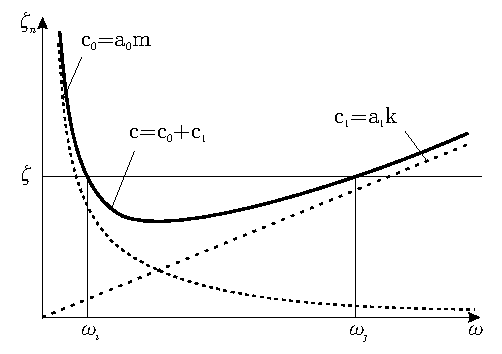
\includegraphics[]{/rayleigh/rayleigh_chart.pdf}
	\captionsetup{justification=centering}
	\caption{Wizualizacja wpływu masy i sztywności na macierz tłumienia według Rayleigh'a}
	\label{fig: rayleigh_chart}
\end{figure}
Z rysunku \ref{fig: rayleigh_chart} można wysnuć przydatne z praktycznego punktu widzenia wnioski. Założone tłumienie $\zeta$ jest spełnione jedynie dla dwóch konkretnych częstości $\omega_i$ i $\omega_j$ użytych w formułach \ref{eq: raileigh_parameters}. Składnik $c_1=a_1 k$ wzrasta liniowo wraz ze wzrostem częstości. Z kolei składnik $c_0 = a_0 m$ maleje nieliniowo wraz ze wzrostem częstości. Sumaryczna wartość obu składników dla przedziału $<\omega_i ,\omega_j>$ jest mniejsza niż zakładana. Z kolei dla częstości spoza przedziału, tłumienie jest większe niż zakładane. Jeżeli przedział interesujących częstości jest dobrany prawidłowo, to takie podejście jest bezpieczne z punktu widzenia projektanta. Jest tak ponieważ, odpowiedź modelu konstrukcji jest zawyżona względem odpowiedzi rzeczywistej struktury \parencite{Oleszek2015}.




%Identyfikacja modalna
\chapter{Identyfikacja cech dynamicznych konstrukcji}

\textit{Streszczenie: W niniejszym rozdziale przytoczono klasyfikację metod analizy modalnej. W dalszej części skupiono uwagę na Operacyjnej Analizie Modalnej. Przedstawiono generalne założenia OMA oraz zastosowania udokumentowane w literaturze. Następnie opisano wybrany do wykorzystania w pracy algorytm NExT-ERA. Przedstawiono jego syntetyczną formę wraz z zaleceniami dotyczącymi użycia. W dalszej części rozdziału opisano stworzoną do identyfikacji modalnej aplikację komputerową korzystającą z algorytmu NExT-ERA. Na końcu przedstawiono testy numeryczne oraz eksperymentalne metody i aplikacji komputerowej.}

\textbf{Przerzucić tutaj wstępu z dynamiki.}

\section{Operacyjna analiza modalna (OMA)}
\subsection{Koncepcja OMA}
W ogólności doświadczalna analiza modalna to proces korelacji charakterystyk dynamicznych modelu matematycznego, z fizycznymi właściwościami systemu opisanego rezultatami pomiarów. Przypomnijmy, że w OMA do procesu estymacji parametrów modalnych używane są tylko pomiary odpowiedzi konstrukcji. Różni ją to od EMA, w której mierzone są zarówno wymuszenia jak i odpowiedź. 
Fundamentem wszystkich metod OMA jest założenie, że badana struktura obciążona jest wymuszeniem o widmie zbliżonym do białego szumu. Oznacza to, żę energia konstrukcji jest rozłożona w szerokim paśmie częstotliwości, które zawiera wszystkie interesuje badacza mody do identyfikacji. Z oczywistych względów idealne wymuszenie o charakterystyce białego szumu nie jest możliwe. Większość metod radzi sobie z tym brakiem, jednak najważniejsze jest, żeby wszystkie interesujące mody były odpowiednio wzbudzone, tak aby ich wkład był wychwycony przez przyrządy pomiarowe. \cite{Brincker2015} tłumaczą tę koncepcję za pomocą fikcyjnego, kolorowego filtru obciążenia. Zaproponowano, że kolorowe obciążenie może być traktowanego jako wynik obciążenia kolorowego filtru (zgodnego z obciążeniem) przez idealnie biały szum. Udowodniono, że takie podejście nie zmienia fizycznych modów systemu. Należy jednak pamiętać, że metody OMA w tym przypadku dokonają identyfikacji modalnej zarówno struktury fizycznej, jak i filtra obciążenia. Koncepcję zaprezentowano na rysunku \ref{fig: color_filter_oma}. Najważniejszą konsekwencją jest możliwość występowania wśród wyników identyfikacji nie tylko modów związanych z konstrukcją, ale też wynikających z warunków obciążenia. Należy pamiętać również, że pomierzone wartości obarczone są szumem pomiarowym. Nie niesie on żadnej istotnej, fizycznej informacji, ale jest nieunikniony w trakcie rzeczywistych pomiarów. Tak więc wynik identyfikacji zawiera w sobie trzy składowe:
\begin{itemize}[noitemsep]
	\item parametry modalne związane z drganiami własnymi konstrukcji,
	\item myślowy filtr obciążenia, kolorujący biały szum do rzeczywistego, nieznanego obciążenia,
	\item szum pomiarowy.
\end{itemize} 
W idealnych warunkach, kiedy filtr obciążenia ma biały kolor, a szum pomiarowy byłby zerowy, OMA zidentyfikuje wyłącznie mody konstrukcji.
\begin{figure}[h] 
	\centering
	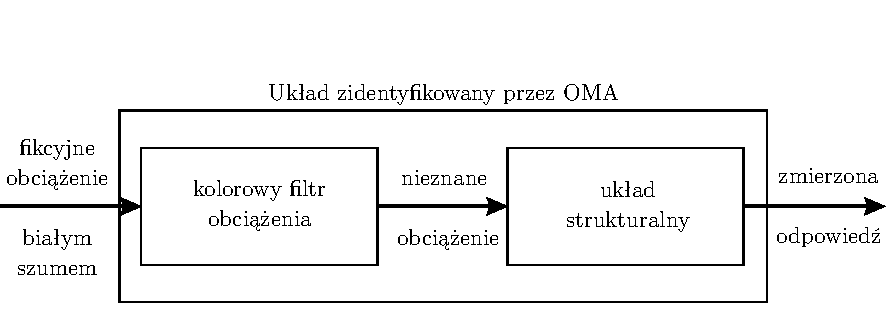
\includegraphics[]{/modal_analysis/filter_coloring.pdf}
	\captionsetup{justification=centering}
	\caption{Schemat układu identyfikowanego przez OMA przy koncepcji kolorowego filtru obciążenia}
	\label{fig: color_filter_oma}
\end{figure}

Operacyjna Analiza Modalna jest obwarowana pewnymi założeniami. Są one rozwinięciem założeń podanych w punkcie \ref{section: modalAnalysisIntro}. Układ poddany analizie OMA musi spełniać następujące warunki:
\begin{itemize}
	\item liniowość - odpowiedź układ na zadaną kombinację obciążeń, jest sumą odpowiedzi odpowiadających każdemu obciążeniu traktowanemu osobno - zasada superpozycji,
	\item stacjonarność - charakterystyki dynamiczne konstrukcji nie zmieniają się w czasie. Innymi słowy, współczynniki równań różniczkowych opisujących odpowiedź struktury są niezależne od czasu.
	\item obserwowalność - dobór lokalizacji punktów pomiarowych musi być tak zaprojektowany, żeby był w stanie dostrzec interesujące obserwatora mody. Niezależnie od tego w trakcie analizy spełnione muszą być również kryteria obserwowalności sterowalności opisane w punkcie \ref{section: hankelMatrix}.
\end{itemize}


\subsection{Metody operacyjnej analizy modalnej}

Metody identyfikacji modalnej dzielą się na dwa główne rodzaje związane z dziedziną w której działa algorytm:
\begin{itemize}[noitemsep]
	\item metody w dziedzinie czasu \teng{time-domain methods (TDM)},
	\item metody w dziedzinie częstotliwości \teng{frequency-domain methods (FDM)}.
\end{itemize}
Metody EMA w dziedzinie czasu wykorzystują do estymacji parametrów modalnych funkcje odpowiedzi impulsowej \teng{inpulse response function (IRF)}. W OMA, nośnikiem informacji o odpowiedzi swobodnej układu \teng{free decays} są funkcje korelacji \teng{correlation functions}. Identyfikacja parametrów polega w tym przypadku na dopasowaniu parametrów modalnych do informacji zawartej w funkcjach korelacji. Stosowane są do tego modele parametryczne wykorzystujące techniki regresji. Główną różnicą pomiędzy dostępnymi algorytmami TD jest właśnie zastosowana metoda regresji. Zasadniczo wszystkie metody TD stosowane w EMA mogą być użyte w OMA właśnie z zastosowaniem funkcji korelacji. 


Podobną analogię jak w metodach TD można zauważyć dla metod w dziedzinie częstotliwości. W algorytmach EMA w dziedzinie częstotliwości bazą do identyfikacji są funkcje odpowiedzi częstotliwościowej \teng{frequency-response function (FRF)}. W OMA rolę tę pełnią funkcje gęstości widmowej \teng{spectral density functions}.

Przed wyborem dziedziny w której badacz chce się poruszać, warto poznać elementy charakterystyczne dla grupy algorytmów TD i FD. Podstawową wadą metod TD jest to, że wszystkie mody, które występują w sygnale są ujęte w funkcjach korelacji. W konsekwencji wszystkie mody zawsze są rozważane w trakcie rozwiązania problemu. Z kolei ich zaletą, w porównaniu do metod FD, jest większa odporność na wystąpienie błędów systematycznych w estymowanych parametrach modalnych. Niejako w kontrze do metod TD, zaletą metod FD jest to, że każdy z modów występuje w wąskim przedziale częstotliwości. Dzięki temu możliwe jest rozważanie tylko przedziałów częstotliwości, w których występują interesujące badacza mody. Z drugiej strony wadą metod FD jest wykorzystywanie do identyfikacji funkcje gęstości widmowej, które są wyznaczane za pomocą różnych metod (CYTOWANIE) obciążonych błędami systematycznymi. Błędy te nieuchronnie przenoszą się na wynikowe parametry modalne, a określenie ich wpływu jest problematyczne. \cite{Maia1997} sugerują, że metody w dziedzinie czasu są z reguły lepszym wyborem w przypadku dużego przedziału interesujących badacza częstotliwości, albo dużej liczby modów w tym zakresie. Natomiast metody w dziedzinie częstotliwości dostarczają lepszych wyników kiedy zakres częstotliwości jest niewielki, a liczba modów relatywnie mała. 

Drugie kryterium podziału algorytmów dotyczy liczby modów, które mogą być jednocześnie analizowane za pomocą danej metody. Podział jest zbliżony do tego dotyczącego teoretycznej analizy modalnej. Metoda może identyfikować albo jeden stopień swobody \teng{single degree-of-freedom} albo wiele stopni swobody \teng{multiple degree-of-freedom}.

Metody TDM i FDM możemy podzielić również na bezpośrednie \teng{direct} i pośrednie \teng{indirect}. Różnica polega na sposobie wyznaczania FRF. Metody bezpośrednie pozwalają wyznaczyć ją bezpośrednio z równania ruchu. Natomiast metody pośrednie estymują FRF na podstawie wcześniej zidentyfikowanego modelu modalnego.

Ostatnim ogólnie przyjętym kryterium podziału jest liczba punktów poddanych wymuszeniu i mierzonych w trakcie serii pomiarowej. Koresponduje to z liczbą analizowanych jednocześnie przez metodę identyfikacji funkcji FRF. Kiedy mówimy o jednoczesnej analizie tylko jednej funkcji FRF mamy do czynienia z metodą jedno-wejście-jedno-wyjście (SISO) \teng{single-input-single-output}. Kiedy mierzymy wymuszenie w jednym punkcie, a odpowiedź badamy w kilku różnych punktach na konstrukcji, otrzymując kilka funkcji FRF, metodę klasyfikuje się jako jedno-wejście-wiele-wyjść (SIMO) \teng{single-input-multi-output}. W powyższej technice obowiązuje założenie, że parametry modalne uzyskane z każdej funkcji FRF będą takie same. Innymi słowy są to parametry globalne dla całej konstrukcji. Naturalnym rozwinięciem są metody które mogą analizować wszystkie dostępne funkcje FRF jednocześnie, uzyskane w skutek wymuszenia i pomiaru wielu różnych punktów. Metody te określane są jako wiele-wejść-wiele-wyjść (MIMO) \teng{multi-input-multi-output}.

\cite{Maia1997} opisali szczegółowo wiele z metod zarówno eksperymentalnej jaki i doświadczalnej analizy modalnej. Z kolei \cite{Brincker2015} sklasyfikowali najpopularniejsze, używane współcześnie metody identyfikacji OMA. Spośród algorytmów działających w dziedzinie czasu należy wymienić:
\begin{itemize}[noitemsep]
	\item Poly Reference (PR) \parencite{Norton2009,Vold1982},
	\item Autoregressive Moving Average (ARMA) \parencite{Shi1987,Huang2000,Giorcelli1994},
	\item Ibrahim Time Domain (ITD) \parencite{Ibrahim1983,Pappa1985a},
	\item Eigensystem Realization Algorithm (ERA) \parencite{Juang1985,Pappa1985,Juang1988},
	\item Stochastic Subspace Identification (SSI). \parencite{VanOverschee1996,Peeters1999a,Peeters2000}. 
\end{itemize}

Warto zaznaczyć, żę metoda ERA przy zastosowaniu postulatów NExT stanowi jeden z pośrednich wariantów metody SSI, używający funkcji korelacji jako źródła informacji przy identyfikacji.

Z kolei najpopularniejsze algorytmy w dziedzinie częstotliwości to:
\begin{itemize}[noitemsep]
	\item Basic Frequency Domain (Peak-Picking) \parencite{Felber1994},
	\item Frequency-Domain-Decomposition (FDD) \parencite{Brincker2000,Brincker2001a,Brincker2001b},
	\item The Least Squares Complex Frequency Method (LSCF) \parencite{Verboven2005},
	\item The Poly-Reference Least Squares Complex Frequency Method (p-LSCF) \parencite{Peeters2005}.
\end{itemize}



Wszystkie z powyższych algorytmów są bardzo dobrze opisane i udokumentowane w literaturze. Trudno orzec, który z nich jest obiektywnie najlepszy. Wiele zależy od doświadczenia i wiedzy autora oraz specyfiki zadania. Jak powiedział Sam Ibrahim: "Jeśli nie występują blisko położone mody i szumy - wszystko zadziała" \teng{"If there are no closely spaced modes and no noise - everything works"}. Wybór metody może więc zależeć od preferencji, umiejętności programowania czy dostępnych narzędzi. W literaturze można napotkać wiele indywidualnych aplikacji algorytów (CYTOWANIE). Istnieją również komercyjne programy, które pozwala na identyfikację modalną. Do najpopularniejszych należą ARTeMIS - SVS \parencite{Extractor1999} i MACEC - dodatek do programu MATLAB \parencite{Reynders2014}.

Do identyfikacji parametrów modalnych konstrukcji, które są częścią tej pracy autor zdecydował o zastosowaniu algorytmu NExT-ERA. Wynika to z doświadczenia zespołu mostów Politechniki Gdańskiej przy stosowaniu tej metody oraz z dostępnej szerokiej literatury pokazującej skuteczne zastosowanie tej metody w przypadku badania mostów. W kolejnym rozdziale omówiono szczegóły metody oraz implementację jej algorytmu w autorskiej aplikacji napisanej w języku Python.

\section{Przykłady zastosowań Operacyjnej Analizy Modalnej}
Operacyjna analiza modalna została zastosowana w wielu przykładach testowych i przy rozwiązaniu rzeczywistych problemów inżynierskich. Identyfikacja OMA najczęściej służy jako element detekcji zmian i uszkodzeń konstrukcji lub jako punkt odniesienia przy kalibracji modeli numerycznych. Ze względu na swoje właściwości używana jest przy badaniu dużych budowli i konstrukcji, których sztuczne wymuszenie byłoby problematyczne. W literaturze można znaleźć wiele przykładów identyfikacji modalnej rzeczywistych mostów \parencite{L.Hermans1999,Siringoringo2008,Degrauwe2008,Liu2009,Bayraktar2009,Brownjohn2010,Dohler2011,Magalhaes2012,Benedettini2015,Brownjohn2017,Brownjohn2018,Poprawa2018,Barbieri2019,Qin2019,Favarelli2021}, turbin wiatrowych \parencite{Carne2010,Sarrafi2018}, budynków \parencite{Zhu2018,Xie2021}, statków powietrznych \parencite{SHEN2003,Moncayo2010} czy budowli wieżowych \parencite{Cabboi2017,Szafranski2020}. 

\section{Metoda NExT-ERA}
Metoda NExT-ERA jest jedną z metod operacyjnej analizy modalnej. Składnik NExT pochodzi od słów \textbf{N}atural \textbf{Ex}citation \textbf{T}echnique. NExT jest właściwie klasą metodą OMA. Zawiera w sobie algorytmy początkowo stworzone do eksperymentalnej analizy modalnej wejście-wyjście \teng{input-output} (np. ERA, LSCE, ITD), a które następnie rozszerzone zostały do analizy problemu jedynie na podstawie sygnałów odpowiedzi konstrukcji \teng{output-only}. Taką możliwość ujawniło odkrycie faktu, że funkcje korelacji odpowiedzi konstrukcji, wywołanej losowymi wymuszeniami mogą być wyrażone jako suma zanikających sinusoid. Potwierdzono również, że funkcje korelacji zawierają informację na temat parametrów modalnych struktury. Zauważono więc, że można zastąpić tradycyjnie używane funkcje odpowiedzi impulsowej (IRF), funkcjami korelacji losowych drgań konstrukcji pod wymuszeniem środowiskowym. W ten sposób tradycyjne metody EMA zostały skutecznie zaadaptowane do OMA \parencite{Rainieri2014}. W dalszej części rozdziału zostaną przedstawione najważniejsze zagadniania dotyczące identyfikacje metodą NExT-ERA. 

\subsection{Funkcje korelacji, a odpowiedź swobodna układu} \label{sect: correlationFunction}
Przyjmijmy, że $X$ oznacza zmienną losową, a $x(t)$ realizację tej zmiennej losowej w czasie. $x(t)$ w tej pracy może być utożsamiany z zaobserwowanym sygnałem. Wprowadźmy prostą definicję kowariancji. Jest to funkcja, która dostarcza informacji o zależności pomiędzy dwoma zmiennymi i dana jest wzorem:
\begin{equation}
	\mathrm{cov}[X,Y] = \mathrm{E}[XY]=\int_{-\infty}^{\infty}\int_{-\infty}^{\infty}xyp_{xy}(x,y)\,dxdy
\end{equation}
gdzie: $\mathrm{E}[\,]$ - wartość oczekiwana, $p_{xy}(x,y)$ - wspólna funkcja gęstości prawdopodobieństwa \teng{joint probability density function}. Używając metody uśredniania w czasie $[0,T]$ możemy zapisać kowariancję jako:
\begin{equation}
	\mathrm{cov}[x(t),y(t)] = \mathrm{E}[x(t)y(t)]=\frac{1}{T}\int_{0}^{T}x(t)y(t) \,dt
\end{equation}
Korelacją możemy określić zależność jak dla kowariancji, w której usunięto czynnik stały (wartość średnią) i opisać równaniem (\ref{eq: correlationDef}). W OMA zwykle sygnały na samym początku analizy są pozbawiane czynnika stałego, stąd użycie właśnie funkcji korelacji jest dla tej rodziny metod analizy modalnej kluczowe.
\begin{equation} \label{eq: correlationDef}
	\mathrm{cor}[x(t),y(t)] = \mathrm{E}[(x(t)-\mu_x)(y(t)-\mu_y)]=\frac{1}{T}\int_{0}^{T}(x(t)-\mu_x)(y_{}(t)-\mu_y) \,dt
\end{equation}

W OMA funkcja korelacji wykorzystywana jest jako autokorelacja \teng{autocorrelation} i cross-korelacja \teng{cross-correlation}. Dla pojedynczego sygnału $x(t)$ można rozważyć jak wygląda korelacja pomiędzy punktem $x(t)$, a punktem $x(t+\tau)$, czyli odległym w czasie o $\tau$. Przedstawienie graficzne problemu pokazano na rysunku \ref{fig: autocorrelationExample}. Intuicyjnie widać, że wartość korelacji dla punktów bliskich sobie będzie duża, a dla punktów bardzo od siebie odległych będzie maleć. Autokorelacją nazwiemy funkcję daną równaniem (\ref{eq: autocorrelationDef}), gdzie funkcję $y$ w równaniu (\ref{eq: correlationDef}) zastąpiono $x(t+\tau)$. 
\begin{figure}[h] 
	\centering
	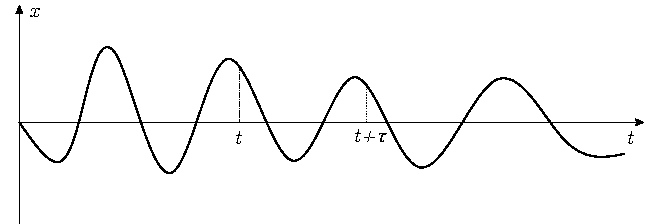
\includegraphics[]{/korelacja/korelacja.pdf}
	\captionsetup{justification=centering}
	\caption{Autokorelacja, jako korelacja wartości funkcji $x(t)$ w czasie $t$ i $t+\tau$}
	\label{fig: autocorrelationExample}
\end{figure}
\begin{equation} \label{eq: autocorrelationDef}
	R_x(\tau)=\mathrm{E}[x(t)x(t+\tau)]
\end{equation}
Funkcję cross-korelacji opiszemy analogicznie jak autokorelacji, z tą różnicą, że pod uwagę weźmiemy dwa losowe sygnały $x(t)$ i $y(t)$.
\begin{equation} \label{eq: crosscorrelationDef}
	\begin{aligned}
		R_{xy}(\tau)=\mathrm{E}[x(t)y(t+\tau)]\\	
		R_{yx}(\tau)=\mathrm{E}[y(t)x(t+\tau)]
	\end{aligned}
\end{equation}

Nie znając funkcji gęstości prawdopodobieństwa, funkcje autokorelacji  i cross-korelacji można wyznaczyć za pomocą uśredniania w czasie co opisano równaniami odpowiednio (\ref{eq: timeAveAutocorrelation}) i (\ref{eq: timeAveCrosscorrelation}). W dalszej części pracy podane zostaną inne przykłady metod wyznaczania funkcji korelacji.
\begin{equation} \label{eq: timeAveAutocorrelation}
	R_x = \frac{1}{T}\int_{0}^{T}x(t)x(t+\tau) \,dt
\end{equation}

\begin{equation} \label{eq: timeAveCrosscorrelation}
	\begin{aligned}
		R_{xy} = \frac{1}{T}\int_{0}^{T}x(t)y(t+\tau) \,dt \\
		R_{yx} = \frac{1}{T}\int_{0}^{T}y(t)x(t+\tau) \,dt 
	\end{aligned}
\end{equation}
Jedną z istotnych właściwości funkcji korelacji jest możliwość wyznaczenia jej przez splot między sygnałem $x(-t)$ i $y(t)$, co zapisano równaniem (\ref{eq: splotCorrelation}). Główną zaletą tego rozwiązania jest prostota obliczeń, ponieważ splot dwóch funkcji jest łatwy do wyznaczenia w dziedzinie częstotliwości \parencite{Brincker2015}.
\begin{equation} \label{eq: splotCorrelation}
	R_{xy}(\tau)=x(-t)*y(t)
\end{equation}
W praktyce wykonywanych jest wiele pomiarów. Załóżmy, że dla zestawu $N$ pomiarów, zmierzone odpowiedzi mogą być zestawione w wektor:
\begin{equation}
	\vect{y}(t) = \{y_1(t),y_2(t),y_3(t), \hdots ,y_N(t)\}^T
\end{equation}
Wyniki autokorelacji i cross-korelacji pomiędzy wszystkimi zmierzonymi sygnałami można zagregować i zapisać macierzowo (\ref{eq: matCorelationDef}). Na przekątnej macierzy znajdują się funkcje autokorelacji, a poza przekątną cross-korelacji.
\begin{equation} \label{eq: matCorelationDef}
	\matr{R}^T(\tau)=\mathrm{E}[\vect{y}(t)\vect{y}^T(t+\tau)]
\end{equation}
Macierzą korelacji \teng{correlation matrix} nazywa się macierz (\ref{eq: matCorelationDef}) dla $\tau=0$ co można zapisać wzorem (\ref{eq: correlationMatrixDef}).
\begin{equation} \label{eq: correlationMatrixDef}
	\matr{C}=\mathrm{E}[\vect{y}(t)\vect{y}^T(t)]=\matr{R}(0)
\end{equation}

Funkcje korelacji posiadają dwie wspomniane wcześniej właściwości kluczowe dla OMA. Po pierwsze teoretycznie pozwalają wyodrębnić wszystkie informacje na temat parametrów modalnych konstrukcji z sygnału losowego. Po drugie mogą być utożsamiane z drganiami swobodnymi, gasnącymi układu \parencite{James1995}. Oba założenia zostały wyjaśnione i udowodnione poniżej.

Założenie o reprezentacji wszystkich parametrów modalnych przez funkcje korelacji opiera się na wykorzystaniu właściwości funkcji korelacji, rozkładu normalnego oraz Centralnego Twierdzenia Granicznego \teng{central limit theorem}. Centralne Twierdzenie Graniczne mówi, że dla niezależnych zmiennych losowych $X_i$ o jednakowym rozkładzie, fluktuujących wokół wartości oczekiwanej $\mu$ i o skończonej wariancji $\sigma^2$ to wyrażenie (\ref{eq:centralLimitTheorem})
\begin{equation} \label{eq:centralLimitTheorem}
	\frac{\frac{1}{n}\sum_{i=1}^{M} X_i - \mu}{\frac{\sigma}{M}}
\end{equation}
zbiega według rozkładu do rozkładu Gaussa przy nieskończonej liczbie M.
\cite{Brincker2015} przedstawili uzasadnienie użycia tego twierdzenia w przypadku OMA w następujący sposób. Rozważmy zestaw zmiennych losowych $\{x_1,x_2,...,x_M\}$, które są niezależne i posiadają identyczny rozkład, ze średnią wartością $\mu$ i wariancją $\sigma^2$. Liniowa kombinacja tych zmiennych losowych jest dana wzorem:
\begin{equation} \label{eq:CLTsum}
	y = \sum_{i=1}^{M} a_i x_i
\end{equation}
Centralne twierdzenie graniczne mówi o tym, że dla dużej liczby zmiennych losowych $M$ rozkład $y$ jest w przybliżeniu normalny, z wartością średnią $\mu_y=\mu\sum a_i$, wariancją $\sigma_y^2=\sigma^2\sum \sigma^2$ i przy $M \xrightarrow{} \infty$ zbiega do rozkładu normalnego. Odwołując się do dynamiki budowli możemy zapisać, że odpowiedź układu $y(t)$ jest splotem siły wymuszającej $x(\tau)$ i funkcji odpowiedzi impulsowej $h(t)$ co pokazano równaniem:
\begin{equation} \label{eq:convolutionResponse}
	y(t)=\int_{-\infty}^{\infty}h(t-\tau)x(\tau) \,d\tau
\end{equation}

Dla sygnału dyskretnego z krokiem czasowym $\Delta t$ i ograniczając się jedynie do $N_m$ istotnych z punktu widzenia pamięci systemu próbek, zależność może być przedstawiona następująco:
\begin{equation}
	y(n) = \sum_{k=n-N_m}^{n} h(n-k)x(k)\Delta t
\end{equation}
Można zauważyć, że dla wymuszenia szumem białym odpowiedź dynamiczna $y(n)$ jest sumą, którą można przedstawić wzorem (\ref{eq:CLTsum}), gdzie poszczególne składniki obciążenia $x(k)$ nie muszą mieć rozkładu normalnego, ale ostateczna odpowiedź będzie mieć rozkład Gaussa. Wynika to wprost z Centralnego Twierdzenia Granicznego. Warto nadmienić, że założenie o wymuszeniu białym szumem zapewnia nam niezależność składników obciążenia $x(k)$. 

Bazując na powyższym, w OMA zwykle zakładamy, że mierzone sygnały posiadają wartość średnią równą zero oraz są Gaussowskie \teng{Gaussian signals} lub bliskie Gaussowskim \parencite{Brincker2015}. Przypomnijmy, że jednowymiarowa funkcja gęstości prawdopodobieństwa rozkładu normalnego dana jest wzorem:
\begin{equation}
	p(x) = \frac{1}{\sqrt{2\pi\sigma^2}}e^{-\frac{(x-\mu)^2}{2\sigma^2}}
\end{equation}
, a przyjmując dodatkowo wartość średnią równą
zero wzór można wyrazić następująco:
\begin{equation} \label{eq:normalDensZeroMean}
	p(x) = \frac{1}{\sqrt{2\pi\sigma^2}}e^{-\frac{x^2}{2\sigma^2}}
\end{equation}
Dla wektora losowego, zawierającego zmienne losowe o zerowej wartości średniej $\vect{x}^T=\{x_1,x_2,x_3,\hdots,x_M\}$, funkcja gęstości prawdopodobieństwa może być zapisana jako:
\begin{equation}\label{eq: normalDistributionCorr}
	p(x) = \frac{1}{(2\pi)^\frac{M}{2} \matr{|C|}}e^{\vect{x}^T\matr{C}^{-1}\vect{x}/2}
\end{equation}
gdzie $|\matr{C}|$ jest wyznacznikiem macierzy korelacji (\ref{eq: correlationMatrixDef}). Podstawowym wnioskiem wynikającym z tej zależności jest to, że jednowymiarowy rozkład Gaussa może być opisany za pomocą średniej wartości, odchylenia standardowego i w przypadku wielowymiarowych danych o zerowej wartości średniej, jedynie przez przez macierz korelacji (\ref{eq: normalDistributionCorr}).

Aby wytłumaczyć dlaczego funkcje korelacji w OMA mogą być odpowiednikiem funkcji odpowiedzi impulsowej (IRF), a funkcje gęstości widmowej odpowiednikami funkcji odpowiedzi częstotliwościowej (FRF) przytoczmy wymagane definicje i zależności z dynamiki budowli. Szczegółowe wyprowadzenia i objaśnienia znajdują się między innymi w pracach \parencite{Brincker2015,Rainieri2014,Chopra2012a,Ewins2000}. Funkcja odpowiedzi impulsowej układu, zwykle oznaczone jako $h(t)$ jest odpowiedzią układu poddanego wymuszeniu przez impulsową siłę, o bardzo krótkim czasie działania, w chwili czasowej $t=0$. Matematycznie impulsową siłę opisuje funkcja nazywaną deltą Diraca $\delta(t)$. Dla systemów liniowych i czasowo niezależnych, jeżeli przesunięta w czasie zostanie chwila przyłożenia impulsu o $\tau$, to otrzymamy odpowiedź $y(t)$, która będzie również przesunięta w czasie o $\tau$. Z definicji wiemy, że impuls jest iloczynem intensywności obciążenia i czasu jego działania. Rozważmy ciągłe obciążenie oznaczone jako $x(t)$, które jest superpozycją potoku impulsów o zmiennej amplitudzie, ale o równie krótkich czasach trwania. W takim przypadku impuls siły od czasu $\tau$ do $\tau+d\tau$ obliczamy jako $x(\tau)d\tau$, a odpowiedź układu jako $h(t-\tau)x(\tau)d\tau$. Układ jest liniowy a więc obowiązuje zasada superpozycji. Wynika z tego, że suma wpływu całego obciążenia może być wyznaczona jako suma wszystkich składowych odpowiedzio i opisana całką Duhamel'a jako (\ref{eq: duhamelIntegralIRF}) oraz w postaci splotu (\ref{eq: convolutionIntegralIRF}) miedzy funkcją IRF $h(t)$ i wymuszeniem $x(t)$.
\begin{equation} \label{eq: duhamelIntegralIRF}
	y(t)=\int_{-\infty}^{\infty} h(t-\tau)x(\tau)d\tau
\end{equation}
\begin{equation} \label{eq: convolutionIntegralIRF}
	y(t)=h(t)*x(t)
\end{equation}
Funkcję IRF można wyznaczyć wykonując przekształcenie Laplace'a równania ruchu przedstwaionego równaniem (\ref{eq: mot_und}). Dla przejrzystości przytoczono je poniżej (\ref{eq: motionIRF}), dla układu z jednym stopniem swobody, wymuszenia deltą Diraca i podstawiając w miejsce odpowiedzi układu funkcję IRF:
\begin{equation} \label{eq: motionIRF}
	m\ddot{h}(t)+c\dot{h}(t)+kh(t)=\delta(t)
\end{equation}
Wykonując transformatę Laplace'a obu stron otrzymamy:
\begin{equation} \label{eq: laplaceTransofrmMOVEQ}
	(ms^2+cs+k)H(s)=1
\end{equation}
Wykorzystując właściwości transformaty i przekształcając odpowiednio równanie (\ref{eq: laplaceTransofrmMOVEQ}) otrzymamy formułę (\ref{eq: laplaceTransofrmMOVEQ2}). Na jej podstawie można wprost wyznaczyć funkcje IRF podaną równaniem (\ref{eq: IRFfunction}).
\begin{equation} \label{eq: laplaceTransofrmMOVEQ2}
	H(s) = \frac{1}{m(s-\lambda)(s-\lambda^*)}
\end{equation}
\begin{equation} \label{eq: IRFfunction}
	h(t)=\frac{1}{m}\frac{e^{\lambda t}-e^{\lambda^*t}}{\lambda-\lambda^*}
\end{equation}



Z kolei funkcja FRF w sensie fizycznym reprezentuje amplitudę i przesunięcie fazowe drgań ustalonych systemu SDOF, poddanego wymuszeniu harmonicznemu o jednostkowej amplitudzie i częstotliwości $\omega_d$. Matematycznie FRF $H(\omega)$ można opisać również jako transformatę Laplace'a z IRF obliczoną dla urojonej współrzędnej $s=i\omega$ (\ref{eq: laplaceTransofrmMOVEQ2}) i zapisać następująco:
\begin{equation} \label{eq: FRFfunction}
	H(\omega)=\frac{1}{m(i\omega-\lambda)(i\omega-\lambda^*)}
\end{equation}
Podobnie jak IRF, FRF łączy wymuszenie z odpowiedzią układu. Jeśli równanie ruchu (\ref{eq: mot_und}) stronami przekształcimy transformatą Fouriera to otrzymamy:
\begin{equation} \label{eq: FRF_moteq}
	(m(i\omega)^2+ci\omega + k)Y(\omega)=X(\omega)
\end{equation}
Szczegółowe rozwiązanie za pomocą reprezentacji biegunów układu można znaleźć w literaturze \parencite{Brincker2015}. Ostatecznie otrzymujemy:
\begin{equation} 
	m(i\omega-\lambda)(i\omega-\lambda^*)Y(\omega)=X(\omega)
\end{equation}
Po przekształceniu wyraźnie widać relację pomiędzy odpowiedzią, a wymuszeniem układu za pośrednictwem FRF:
\begin{equation} \label{eq: FRF_final}
	Y(\omega)=\frac{1}{m(i\omega-\lambda)(i\omega-\lambda^*)}X(\omega)=H(\omega)X(\omega)
\end{equation}
gdzie $X(\omega)$ i $Y(\omega)$ są odpowiednio transformatami Fouriera wymuszenia $x(t)$ i odpowiedzi $y(t)$ układu. Porównując równania (\ref{eq: FRF_moteq})(\ref{eq: FRF_final}) łatwo można zauważyć że FRF zawiera w sobie informację na temat bezwładności, tłumienia i sztywności układu.




Zarówno IRF jak i FRF można uogólnić do układów MDOF o $N$ stopniach swobody. Zapis zależności wymuszenie-odpowiedź dla układu MIMO (wiele-wejść-wiele-wyjść) przedstawiono dla dziedziny czasu (\ref{eq: mimoIRFyx}) i częstotliwości (\ref{eq: mimoFRFyx}).

\begin{equation} \label{eq: mimoIRFyx}
	\vect{y}(t)=\matr{H}(t)*\vect{x}(t)
\end{equation}
\begin{equation} \label{eq: mimoFRFyx}
	\vect{\tilde{y}}(\omega)=\matr{\tilde{H}}(i\omega)\vect{\tilde{x}}(\omega)
\end{equation}
gdzie $\matr{H}(t)$ jest macierzą zawierającą funkcje IRF, $\vect{x}(t)$ jest wektorem sił wymuszających, $\vect{\tilde{y}}(\omega)$ i $\vect{\tilde{x}}(\omega)$ są transformatami Fouriera odpowiednio $\vect{x}(t)$ i $\vect{y}(t)$, a $\matr{\tilde{H}}(i\omega)$ jest macierzą FRF. Wyrażenia na odpowiednio IRF $\matr{H}(t)$ i FRF $\matr{\tilde{H}}(i\omega)$ podano poniżej.
\begin{equation} \label{eq: IRFmimo}
	\matr{H}(t)=\sum_{n=1}^{N}(\vect{A}_n e^{\lambda_n t} + \vect{A}_n^* e^{\lambda_n t})
\end{equation} 
\begin{equation} \label{eq: FRFmimo}
	\matr{\tilde{H}}(i\omega)=\sum_{n=1}^{N}(\frac{\vect{A}_n}{i\omega-\lambda_n} + \frac{\vect{A}_n^*}{i\omega-\lambda_n^*})
\end{equation}
gdzie $\vect{A}_n=Q_n \vect{\psi}_n\vect{\psi}_n^T$, $\vect{\psi}_n$ to n-ta postać drgań własnych, $Q_n$ to współczynnik skalujący mody, a $\lambda_n=\sigma_n+i\omega_{d,n}$ jest n-tym biegunem układu zawierającym informacje na temat częstotliwości drgań własnych tłumionych $f_{d,n}=\omega_{d,n}/(2\pi)$ i liczby tłumienia $\xi_r=-\sigma_n/\sqrt{\sigma_n^2+\omega_{d,n}^2}$ n-tego moda.






Gęstość widmowa jest kolejnym kluczowym pojęciem potrzebnym do pełnego zrozumieniu znaczenia funkcji korelacji dla OMA. Gęstość widmowa \teng{auto spectral density} dla przebiegu czasowego $x(t)$ jest zdefiniowana jako transformata Fouriera z funkcji korelacji $R_x(\tau)$ \ref{eq: spectralDensity}. Istnieje również zależność odwrotna, w której odwrotną transformata Fouriera z gęstości widmowej pozwala otrzymać funkcję korelacji \ref{eq: correlationInversSpectralDensity}. Początkowy wyraz funkcji korelacji $R_x(0)$ jest reprezentacją twierdzenia Parsevela i pozwala stwierdzić, że gęstość widmowa pokazuje rozkład energii w funkcji częstotliwości. Stąd gęstość widmową nazywa się również zamiennie gęstością widmową mocy \teng{power spectral density} (PSD) \parencite{Brincker2015}.
\begin{equation} \label{eq: spectralDensity}
	G_x(\omega) = \frac{1}{2\pi}\int_{-\infty}^{\infty}R_x(\tau)e^{-i\omega\tau}\,d\tau
\end{equation}
\begin{equation} \label{eq: correlationInversSpectralDensity}
	R_x(\omega) = \int_{-\infty}^{\infty}G_x(\omega)e^{i\omega\tau}\,d\omega
\end{equation}
Podobnie zdefiniować można gęstość widmową pomiędzy dwoma sygnałami $x(t)$ i $y(t)$ \teng{cross spectral density}, jako przekształcenie Fouriera funkcji cross-korelacji $R_{xy}(t)$. 

\begin{equation} \label{eq: crossspectralDensity}
	G_{xy}(\omega) = \frac{1}{2\pi}\int_{-\infty}^{\infty}R_{xy}(\tau)e^{-i\omega\tau}\,d\tau
\end{equation}
\begin{equation} \label{eq: crosscorrelationInversSpectralDensity}
	R_{xy}(\omega) = \int_{-\infty}^{\infty}G_{xy}(\omega)e^{i\omega\tau}\,d\omega
\end{equation}
Wykorzystanie właściwości splotu funkcji korelacji (\ref{eq: splotCorrelation}) i  splotu\footnote{Transformata Fouriera splotu dwóch funkcji w dziedzinie czasu $h(t)$ i $g(t)$ jest równa iloczynowi transformat Fouriera każdej z funkcji osobno. Innymi słowy transformacie Fouriera wyrażenia $h(t)*g(t)$ odpowiada iloczyn $H_k G_k$, gdzie: $H_k$ - transformata Fouriera funkcji $h(t)$, $G_k$ - transformata Fouriera funkcji $g(t)$.} oraz symetrii Hermitowskiej\footnote{Jeżeli $H(\omega)$ jest transformatą Fouriera rzeczywistej funkcji $h(t)$, to prawdziwe jest równanie $H(\omega)=H^*(-\omega)$. Równanie to jest nazywane symetrią Hermitowską \parencite{Boashash2015}.} transformaty Fouriera pozwala uzyskać następującą właściwość gęstości widmowej (\ref{eq: specDensSplot}). Należy nadmienić, że zależność ta będzie spełniona przy założeniu okresowego (lub bardzo długiego) sygnału \parencite{Brincker2015}.
\begin{equation} \label{eq: specDensSplot}
	G_{xy}(\omega) = X^*(\omega)Y(\omega)
\end{equation}


Rozważamy ponownie układ SISO o odpowiedzi $y(t)$ przy wzbudzeniu $x(t)$: $y(t)=x(t)*h(t)$ (\ref{eq: convolutionIntegralIRF}). Wykorzystując równanie (\ref{eq: specDensSplot}) zapiszemy równanie na gęstość widmową odpowiedzi:
\begin{equation} \label{g}
	G_{y}(\omega) = Y^*(\omega)Y(\omega)
\end{equation}
Wykorzystując transformatę Fouriera oraz przemienność i łączność splotu zapisać można następujące równanie pokazujące zależność pomiędzy gęstością widmową odpowiedzi i wymuszenia układu.
\begin{equation} \label{eq: sisofundamentaltheorem}
	G_{y}(\omega) = G_x(\omega)|H^*(i\omega)|^2
\end{equation}
Równanie (\ref{eq: sisofundamentaltheorem}) jest nazywane twierdzeniem podstawowym \teng{fundamental theorem} metody OMA. Dla układu MIMO twierdzenie to przyjmuje następującą formę w dziedzinie częstotliwości:
\begin{equation} \label{eq: matrixoutputspectraldensity}
	\begin{split}
		\matr{G}_{y}(\omega) &=\matr{\tilde{H}}^*(i\omega)\matr{G}_x(\omega)\matr{\tilde{H}}^T(i\omega)\\
		&=\matr{\tilde{H}}^*(i\omega)\matr{G}_x(\omega)\matr{\tilde{H}}^T(i\omega)
	\end{split}
\end{equation}
z kolei w dziedzinie czasu odpowiadająca macierz korelacji przedstawia się następująco:
\begin{equation} \label{eq: matrixoutputcorrelation}
	\matr{R}_y(\tau)=\matr{H}(-\tau)*\matr{R}_x(\tau)*\matr{H}^T(\tau)
\end{equation}

Jak już wielokrotnie wspomniano, w OMA zakłada się wymuszenie Gaussowskim, stacjonarnym szumem białym o zerowej wartości średniej. Podstawowym efektem tego założenia wymuszenia $x(t)$ w postaci białego szumu jest brak korelacji pomiędzy wymuszeniem w chwili $t$ i w chwili $t+\tau$. Wyjątkiem jest przypadek $\tau=0$. Stąd sygnał posiada zerową wartość średnią, a funkcja korelacji jest deltą Diraca co zapiszemy:
\begin{equation}
	R_x(\tau)=\mathrm{E}[x(t)x(t+\tau)] = 2\pi G_{x0} \delta(\tau)
\end{equation} 
gdzie $G_{x0}$ jest współczynnikiem skalującym. Zakładając dalej, że biały szum działa jedynie w ograniczonym spektrum od $0$ do $B$, a $\sigma_x^2$ to niezmiennie wariancja sygnału, otrzymamy przekształconą wersję () funkcji korelacji. Na jej podstawie można stwierdzić, że PSD wymuszenia (będąca transformatą Fouriera funkcji korelacji) jest wartością stałą\footnote{Transformata Fouriera delty Diraca jest równa jedności: $\int_{-\infty}^{\infty} \delta(t) e^{i\omega t}\,dt = e^{-i\omega\times 0}=1$ \parencite{Zielinski2002}} .
\begin{equation} \label{eq: whitenoisecorrelationSISO}
	R_x(\tau)=2\pi \frac{\sigma_x^2}{2B} \delta(\tau)
\end{equation} 

Chcąc rozwinąć tę zależność do układu MIMO załóżmy sygnały wymuszenia $x_1(t)$ i $x_2(t)$ jako szumy białe. Sformułowanie macierzy korelacji z wykorzystaniem równania (\ref{eq: whitenoisecorrelationSISO}) prowadzi do następującej zależności:
\begin{equation} \label{eq: whitenoisecorrelationMIMO}
	\matr{R}_x(\tau)=\mathrm{E}[\vect{x}(t)\vect{x}^T(t+\tau)]=2\pi \frac{\delta(\tau)}{2B}\matr{C}
\end{equation} 
gdzie $\matr{C}$ jest macierzą kowariancji sygnałów. Macierz gęstości widmowej sygnałów wymuszenia szumem białym ma postać:
\begin{equation} \label{eq: spectraldensitymatrixWHITENOISE}
	\matr{G}_x(\omega)=\begin{cases}
		\frac{\matr{C}}{2B}, & 0\le\omega\le B\\
		0, & \omega>B
	\end{cases}
\end{equation} 


Podsumowując powyższy ciąg myślowy możliwa jest dekompozycja równania (\ref{eq: matrixoutputcorrelation}) w dziedzinie czasu i równania (\ref{eq: matrixoutputspectraldensity}) w dziedzinie częstotliwości. Dekompozycję w dziedzinie czasu przeprowadzili po raz pierwszy \cite{James1993,James1995}. Z kolei dekompozycję w dziedzinie częstotliwości przedstawili \cite{Brincker2000,Brincker2001a}. W powyższych pracach przedstawiono pełny tok postępowania. Poniżej przytoczono rezultaty końcowe w postaci opisu macierzy korelacji sygnałów odpowiedzi układu (\ref{eq: decomposedRx}) i macierzy korelacji gęstości widmowej odpowiedzi (\ref{eq: decomposedGx}).

\begin{equation} \label{eq: decomposedRx}
	\matr{R}_y(\tau)=\begin{cases}
		\sum_{n=1}^{N} (\vect{\phi_n}{\vect{\gamma}_n}^Te^{\lambda_n \tau} + \vect{\phi_n}^*{\vect{\gamma}_n}^He^{\lambda_n^* \tau}), & \tau\ge 0\\
		\sum_{n=1}^{N} (\vect{\gamma_n}{\vect{\phi}_n}^Te^{-\lambda_n |\tau|} + \vect{\gamma_n}^*{\vect{\phi}_n}^He^{-\lambda_n^* |\tau|}), & \tau< 0.
	\end{cases}
\end{equation} 

\begin{equation} \label{eq: decomposedGx}
	\matr{G}_y(\omega)=\sum_{n=1}^{N}\frac{\vect{\phi_n}{\vect{\gamma}_n}^T}{i\omega-\lambda_r}+\frac{\vect{\phi_n}^*{\vect{\gamma}_n}^H}{i\omega-\lambda_r^*}+\frac{{\vect{\gamma}_n}\vect{\phi_n}^T}{-i\omega-\lambda_r}+\frac{{\vect{\gamma}_n}^*\vect{\phi_n}^H}{-i\omega-\lambda_r^*}
\end{equation} 


gdzie oznaczenia przyjęto jak w równaniach (\ref{eq: IRFmimo}) i (\ref{eq: FRFmimo}), a $\vect{\gamma}_n$ oznacza wektor referencyjny związany z n-tym modem. Wektor ten zależny jest od wszystkich parametrów modalnych systemu oraz lokalizacji i macierzy korelacji wymuszeń \parencite{Rainieri2014, Peeters2000}. 

Równanie (\ref{eq: decomposedRx}) pokazuje, że funkcje korelacji odpowiedzi mogą być wyrażone za pomocą sumy zespolonych funkcji eksponencjalnych. \cite{SHEN2003} wskazują na podobieństwo jego formy do równania (\ref{eq: IRFmimo}). \cite{Kennedy1995}, w swojej kluczowej dla metody NExT pracy, rozwinęli to równanie do postaci ukazującej funkcję korelacji jako sumę zanikających sinusoid, o charakterystyce takiej samej jak w przypadku IRF. Podsumowując, funkcje korelacji mogą być użyte jako funkcje odpowiedzi impulsowej (IRF) w metodach TD identyfikacji parametrów modalnych.


\subsection{Eigenystem Realization Algorithm}
Metoda ERA została opracowana w latach 80' XX w. przez naukowców z NASA Langley Research Center: Richarda Pappa i Jer-Nan Juang'a. Przedstawili oni koncept identyfikacji modalnej i redukcji modelu układu dynamicznego na podstawie danych pomiarowych. Nowością, którą wprowadzili autorzy było połączenie pojęć z teorii kontroli i algorytmu rozkładu względem wartości osobliwych. Fundamentalne prace opisujące metodą zostały opisane w \parencite{Pappa1985,Juang1985,Juang1988,Juang1994}. Algorytm ERA był wielokrotnie testowany, na przykaład pod względem odporności na zaszumienie danych pomiarowych \parencite{Juang1986, Li2011}. Spośród polskich autorów, szczegółowy opis metody zawarli w swoich pracach \cite{Szafranski2013} i \cite{Dudek2008}.

\subsubsection{Liniowy model dynamiczny w przestrzeni stanów}
Model przestrzeni stanów\footnote{Według \cite{Kaczorek2016} stanem układu nazywamy zbiór liniowo niezależnych wielkości $x_1, x_2, x_3,\dots,x_n$ określających w pełni skutki przeszłych oddziaływań $(t<t_0)$ na układ, który jest wystarczający do wyznaczenie przebiegów chwilowych dowolnych wielkości w tym układzie dla $t>t_0$, gdy znane są wymuszenia i parametry obwodu. Wielkości $x_1, x_2, x_3,\dots,x_n$ nazywa się zmiennymi stanu, a wektor $\vect{x}=[x_1, x_2, x_3,\dots,x_n]$ wektorem stanu tego obwodu.} \teng{state-space model} używany jest do przekształcenia równania różniczkowego drugiego rzędu (\ref{eq: mot_dam}), do dwóch równań rzędu pierwszego.     Dla przejrzystości macierzowe równanie ruchu przytoczono ponownie poniżej:
\begin{equation}
	\vect{M} \vect{\ddot{x}}(t) +\vect{C} \vect{\dot{x}}(t)+ \vect{Kx}(t) = \vect{F}(t)
\end{equation}
gdzie: $\vect{M}$, $\vect{C}$, $\vect{K}$ to odpowiednio macierze mas, tłumienia i sztywności, $\vect{x}(t)$ jest wektorem przemieszczenia, a $\vect{F}(t)$ jest wektorem wymuszenia. 
Wektor wymuszenia można poddać faktoryzacji do macierzy $\vect{\bar{B}}$ oraz wektora $\vect{u}(t)$ (\ref{eq: }). Macierz $\vect{\bar{B}}$ opisuje lokalizację punków wymuszenia, a wektor $\vect{u}(t)$ intensywność tego wymuszenia w funkcji czasu.
\begin{equation}
	\vect{F}(t) = \vect{\bar{B}}\vect{u}(t)
\end{equation} 
Macierzowe równanie ruchu może być więc przekształcone następująco:
\begin{equation} \label{eq: STATEmanipulated_mot_eq}
	\vect{\ddot{x}}(t) +\vect{M}^{-1} \vect{C} \vect{\dot{x}}(t)+ \vect{M}^{-1}\vect{Kx}(t) = \vect{M}^{-1}\vect{\bar{B}}\vect{u}(t)
\end{equation}
Zdefiniujmy wektor stanu jako:
\begin{equation} \label{eq: stateVector}
	\vect{s}(t) = \begin{Bmatrix}
		\vect{\dot{x}}(t) \\
		\vect{x}(t)
	\end{Bmatrix}
\end{equation}
Liczba komponentów tworzących wektor stanu jest nazywana rzędem modelu. Podstawiając go do równania (\ref{eq: STATEmanipulated_mot_eq}) dodatkowo wykorzystując oczywistą równość $\vect{M}\vect{\dot{x}}(t)=\vect{M}\vect{\dot{x}}(t)$ otrzymamy:
\begin{equation}
	\vect{\dot{s}}(t) = 
	\begin{bmatrix}
		-\vect{M}^{-1}\vect{C} & -\vect{M}^{-1}\vect{K} \\
		\vect{I} & \vect{0}
	\end{bmatrix} \vect{s}(t) + 
	\begin{bmatrix}
		-\vect{M}^{-1}\vect{\bar{B}} \\
		\vect{0}
	\end{bmatrix} \vect{u}(t)
\end{equation}
Stąd możemy zdefiniować następujące macierze: $\vect{A}_c$ i $\vect{B}_c$:
\begin{equation}
	\vect{A}_c = 
	\begin{bmatrix}
		-\vect{M}^{-1}\vect{C} & -\vect{M}^{-1}\vect{K} \\
		\vect{I} & \vect{0}
	\end{bmatrix} 
\end{equation}
\begin{equation}
	\vect{B}_c = 
	\begin{bmatrix}
		-\vect{M}^{-1}\vect{\bar{B}} \\
		\vect{0}
	\end{bmatrix}\phantom{\qquad\qquad\quad}
\end{equation}
Dzięki tak sformułowanym elementom zapiszmy równanie stanu \teng{state equation} następująco:
\begin{equation} \label{eq: stateEquation}
	\vect{\dot{s}}(t)= \vect{A}_c\vect{s}(t)+\vect{B}_c\vect{u}(t)
\end{equation}
W równaniu (\ref{eq: stateEquation}) $\vect{s}(t)$ jest wektorem stanu (\ref{eq: stateVector}), czyli zestawem wielkości opisujących w sposób jednoznaczny stan modelowanego układu, a $\vect{u}(t)$ jest wektorem wejścia (sterowania) i opisuje sygnał wejściowy. Macierze $\vect{A}_c$ i $\vect{B}_c$, nazywane są odpowiednio macierzą stanu (systemu) \teng{state matrix} i macierzą wejścia \teng{input influecne matrix}. Są to macierze stałych współczynników, które odwzorowują modelowany układ dynamiczny i parametry elementów tworzących ten układ.

Drugim równaniem pozwalającym na stworzenie modelu w przestrzeni stanów jest równanie obserwacji \teng{observation equation} lub inaczej równanie wyjścia. W ogólności ma ono postać:
\begin{equation} \label{eq: observationEquationCont}
	\vect{y}(t) = \vect{C_a}\vect{\ddot{x}}(t) + \vect{C_v}\vect{\dot{x}}(t) +\vect{C_d}\vect{x}(t)
\end{equation}
gdzie: $\vect{y}(t)$ jest wektorem mierzonej odpowiedzi w $m$ punktach pomiarowych, a $\vect{\ddot{x}}(t)$, $\vect{\dot{x}}(t)$ i $\vect{x}(t)$ to odpowiednio mierzone przyspieszenia, prędkości i przemieszczenia w danych $m$ punktach. Z kolei macierze $\vect{C_a}$, $\vect{C_v}$ i $\vect{C_d}$ określają lokalizację mierzonych, odpowiadających im przyspieszeń, prędkości i przemieszczeń. Należy zaznaczyć, że rzeczywista konstrukcja składa się z nieskończonej liczby stopni swobody. Nawet w przypadku dyskretyzacji do układu MDOF, jak to ma miejsce w przypadku obliczeń numerycznych, liczba stopni swobody jest ogromna. Z tego względu, w trakcie pomiarów znacznie redukuje się liczbę mierzonych stopni swobody właśnie do $m$. Podstawiając równanie (\ref{eq: STATEmanipulated_mot_eq}) do (\ref{eq: observationEquationCont}), po przekształceniach można otrzymać następujące równanie obserwacji:
\begin{equation} \label{eq: observationEquation}
	\vect{y}(t) = \vect{C}_c\vect{s}(t)+\vect{D}_c\vect{u}(t)
\end{equation}
w którym:
\begin{equation}
	\vect{C}_c = 
	\begin{bmatrix} 
		\vect{C}_v-\vect{C}_a\vect{M}^{-1}\vect{C}  &  \vect{C}_d-\vect{C}_a\vect{M}^{-1}\vect{K}
	\end{bmatrix}
\end{equation}
\begin{equation}
	\vect{D}_c = \vect{C}_a\vect{M}^{-1}\vect{\bar{B}} \phantom{\qquad\qquad\qquad\qquad\qquad\quad.}
\end{equation}
Macierz $\vect{C}_c$ jest nazywana macierzą wyjścia \teng{output influence matrix}, a $\vect{D}_c$ macierzą przenoszenia lub transmisyjną \teng{direct transmission matrix}. Równania stanu (\ref{eq: stateEquation}) i obserwacji (\ref{eq: observationEquation}) łącznie tworzą ciągły, deterministyczny model przestrzeni stanów:
\begin{equation} \label{eq: con_state_space_model}
	\begin{aligned}
		\vect{\dot{s}}(t)= \vect{A}_c\vect{s}(t)+\vect{B}_c\vect{u}(t) \\
		\vect{y}(t) = \vect{C}_c\vect{s}(t)+\vect{D}_c\vect{u}(t)
	\end{aligned}
\end{equation}

Wielkości mierzone w trakcie eksperymentu są próbkowane jedynie w dyskretnych chwilach czasowych. W takim razie, naturalnym dla rzeczywistych zastosowań jest przekształcenie modelu ciągłego przestrzeni stanów w model dyskretny. Zakładając stały czas próbkowania równy $\Delta t$, równania ciągłe mogą być zdyskretyzowane i rozwiązane jedynie w chwilach czasowych $t_k=k\Delta t$ dla $k\in N$. Dla poprawności zapisu dyskretnego, wymagane jest założenie o stałych wartościach elementów wektora wejścia $\vect{u}(t)$ w trakcie pojedynczego kroku czasowego, tj. $\vect{u}(t)=\vect{u}_k$ dla $t \in [k\Delta t, (k+1)\Delta t]$. Przy spełnieniu powyższych założeń możemy zapisać dyskretny model przestrzeni stanów:
\begin{equation} \label{eq: dis_state_space_model}
	\begin{aligned}
		\vect{\dot{s}}_{k+1}= \vect{A}\vect{s}_k+\vect{B}\vect{u}_k \\
		\vect{y}_k = \vect{C}\vect{s}_k+\vect{D}\vect{u}_k
	\end{aligned}
\end{equation}
gdzie macierze $\vect{A}$, $\vect{B}$, $\vect{C}$, $\vect{D}$ są odpowiednio macierzami stanu, wejścia, wyjścia i przenoszenia dla dyskretnego modelu przestrzeni stanów.

\subsubsection{Odpowiedź impulsowa w przestrzeni stanów}
Przyjmijmy układ dynamiczny opisany równaniem (\ref{eq: dis_state_space_model}), w którym $\vect{s}_k$ - jest n-wymiarowym wektorem stan, $\vect{u}_k$ - m-wymiarowym wektorem sterowania, a $\vect{y}_k$ - p-wymiarowym wektorem obserwacji. Parametry Markova takiego systemu $\vect{G}_k$ można zdefiniować następująco \parencite{Schutter2000}:
\begin{equation} \label{eq: markovParameters}
	\vect{G}_k= \begin{cases}
		\vect{D}, & \text{dla }k=0 \\
		\vect{C}\vect{A}^{k-1}\vect{B}, & \text{dla }k=1,2, \dots
	\end{cases}
\end{equation}
Jeżeli spełnione jest równanie (\ref{eq: markovParameters}) to zestaw macierzy $\vect{A}$, $\vect{B}$, $\vect{C}$, $\vect{D}$ jest realizacją łańcucha $G(k)\; \text{dla } k=1,2\dots,\infty$. Realizację nazywa się minimalną, kiedy rząd modelu jest minimalny (\ref{eq: stateVector}).

Zakładając warunek początkowy $\vect{s}(0)=\vect{0}$ i wymuszenie wszystkich punktów układu jednostkowym impulsem w postaci:
\begin{equation}
	\delta_k = \begin{cases}
		1, & \text{dla }k=0 \\
		0, & \text{dla } k>0 
	\end{cases}
\end{equation}
otrzymamy odpowiedź układu postaci:
\begin{equation} \label{eq: impulseInputLTI}
	\vect{Y}_k= \begin{cases}
		\vect{D}, & \text{dla }k=0 \\
		\vect{C}\vect{A}^{k-1}\vect{B}, & \text{dla }k=1,2, \dots
	\end{cases}
\end{equation}
Równanie (\ref{eq: impulseInputLTI}) nazywa się odpowiedzią impulsową układu. Można zauważyć, że elementy sekwencji parametrów Markova odpowiadają wprost elementom odpowiedzi impulsowej układu \parencite{Phan1991}.
W przypadku identyfikacji modalnej rzeczywistej konstrukcji wyznaczenie macierzy opisujących układ jest celem. Dysponując pomierzonym sygnałem odpowiedzi swobodnej (wzbudzonej impulsem) możliwe jest sformułowanie parametrów Markova i poszukiwanie rozwiązania w postaci macierzy układu. W przypadku OMA odpowiedź impulsowa układu może być zastąpiona funkcjami korelacji co udowodniono w (\ref{sect: correlationFunction}).
Niezależnie od źródła danych, sygnały można złożyć w parametry Markova w identyczny sposób. W dalszej części wywodu elementy algorytmu ERA opisywane będą w sposób tradycyjny, operując na sygnale z odpowiedzi swobodnej układu. 

Załóżmy, że $y_k^i$ jest odpowiedzią konstrukcji w chwili czasowej $k\Delta t$, zmierzoną w punkcie pomiarowym $n$, jednym z wszystkich $m$ punktów pomiarowych. Parametry Markova $\vect{Y}_k$ zdefiniujemy zestawiając odpowiedź układu z wszystkich punktów pomiarowych dla danej chwili czasowej $k\Delta t$:
\begin{equation}
	\vect{Y}_k = \begin{Bmatrix}
		y_k^1 \\ y_k^2 \\ y_k^3 \\ \vdots \\ y_k^m 
	\end{Bmatrix},
	\qquad \text{dla } k=1,2,3,\dots
\end{equation}
\subsubsection{Sformułowanie macierzy Hankela} \label{section: hankelMatrix}
Algorytm metody ERA rozpoczyna się od sformułowania uogólnionej, blokowej\footnote{Macierz blokową można opisać jako macierz złożoną z innych macierzy. Na przykład mając 4 macierze $N \times N$: $\vect{A}_1$, $\vect{A}_2$, $\vect{A}_3$, $\vect{A}_4$, można sformułować macierz $2N\times2N$ postaci $\vect{A}=\big[\begin{smallmatrix}
		\vect{A}_1 & \vect{A}_2\\
		\vect{A}_3 & \vect{A}_4
	\end{smallmatrix}\big]$, która posiada dwa blokowe wiersze i dwie blokowe kolumny.
}  
macierzy Hankela\footnote{W ogólności macierzą Hankela nazywamy taką macierz $\vect{A}$ o wymiarach $r\times s$, że spełniona jest równość: $\vect{A_{r+1,s-1}}=\vect{A_{r-1,s+1}}$ 
} 
dyskretnego układu dynamicznego $\vect{H}$ o wymiarach $r\times s$. Wymiary $r$ i $s$ nazywane są parametrami projektowymi \parencite{Szafranski2013} i oznaczają: $r$ - liczbę blokowych wierszy, $s$ - liczbę blokowych kolumn macierzy Hankela. Jeżeli spełnione są warunki $s>n$ i $r>n$ to właściwością macierzy Hankela jest to, że w przypadku pomiarów pozbawionych szumów rząd macierzy Hankela jest równy rzędowi systemu oraz dwukrotnej liczbie modów systemu.
\begin{equation} \label{eq: genericHankelMatrix}
	\begin{split}
		\vect{H}_{k-1}&=\begin{bmatrix}
			\vect{Y}_k		&	\vect{Y}_{k+1} 	& \dots	& \vect{Y}_{k+s-1} \\
			\vect{Y}_{k+1}	&	\vect{Y}_{k+2}	& \dots	& \vect{Y}_{1+k+s-1} \\
			\vect{Y}_{k+2}	&	\vect{Y}_{k+3} 	& \dots	& \vect{Y}_{2+k+s-1} \\	
			\vdots			&	\vdots			& \ddots & \vdots\\
			\vect{Y}_{r-1+k}	&	\vect{Y}_{r-1+k+1} 	& \dots	& \vect{Y}_{r-1+k+s-1} 	
		\end{bmatrix} \\ 
		&= \begin{bmatrix}
			\vect{C}\vect{A}^{k-1}\vect{B}	&	\vect{C}\vect{A}^{k}\vect{B} 	& \dots	 & \vect{C}\vect{A}^{k+s-2}\vect{B} \\
			\vect{C}\vect{A}^{k}\vect{B}	&	\vect{C}\vect{A}^{k+1}\vect{B} 	& \dots	 & \vect{C}\vect{A}^{k+1+s-2}\vect{B} \\
			\vect{C}\vect{A}^{k+1}\vect{B}	&	\vect{C}\vect{A}^{k+2}\vect{B} 	& \dots	 & \vect{C}\vect{A}^{k+3+s-2}\vect{B} \\	
			\vdots							&	\vdots							& \ddots & \vdots\\
			\vect{C}\vect{A}^{r-2+k}\vect{B}	&	\vect{C}\vect{A}^{r-2+k+1}\vect{B} 	& \dots	 & \vect{C}\vect{A}^{r+k+s-3}\vect{B} 	
		\end{bmatrix}\in \mathcal{R}^{rm\times sp}\\
		&= \vect{P}_r \vect{A}^{k-1}\vect{Q}_s\qquad \text{dla } k\ge 1
	\end{split}
\end{equation}
Macierze $P_r$ i $Q_s$ to odpowiednio macierze obserwacji i sterowania układu i są zdefiniowane następująco:
\begin{equation}
	\vect{P}_r = \begin{bmatrix}
		\vect{C} \\ 
		\vect{CA} \\
		\vect{CA}^2\\
		\vdots \\
		\vect{CA}^{r-1}\\
	\end{bmatrix}
	\qquad
	\vect{Q}_s = \begin{bmatrix}
		\vect{B} & \vect{AB} & \vect{A}^2\vect{B} & \dots & \vect{A}^{s-1}\vect{B}    
	\end{bmatrix}	
\end{equation}
Problem wyboru wartości parametrów $s$ i $r$ nie jest ściśle rozwiązany. Zestawienie różnych badań dotyczących doboru parametrów projektowych przedstawił w pracy \cite{Szafranski2013}. Na pewno należy spełnić zależność $s>n$ i $r>n$. Z uwagi na występowanie w sygnale pomiarowym szumów i niepewności związanych ze wstępnym oszacowaniem rzędu modelu parametry trzeba zawyżyć. Jednym z powszechniej używanych zaleceń jest przyjęcie $r=(5\div10)n$ $s=(2\div3)r$ \parencite{Dudek2008}. Część badaczy zaleca aby parametr $s$ dobrać tak, żeby macierz Hankela zawierała większość lub wszystkie parametry Markova odpowiadające wyraźnemu sygnałowi $s = (\frac{2}{3}\div 1)N_s-r-2$ gdzie $N_s$ oznacza liczbę próbek wyraźnego sygnału \parencite{Caicedo2011,Nayeri2009}.

\subsubsection{Realizacja minimalna modelu w przestrzeni stanów}

Jak już wspomniano realizacją układu nazywamy zestaw macierzy $(\vect{A},\vect{B},\vect{C},\vect{D})$. Podstawowym zdaniem jest znalezienie takiej realizacji, dla której zmierzona odpowiedź układu będzie możliwa od odtworzenia przez równania modelu w przestrzeni stanów. W przypadku odpowiedzi swobodnej, nie ma miejsca dodatkowe wymuszenie w trakcie pomiaru, więc prawdziwa jest zależność $\vect{D}=\vect{Y}_0$. Wszystkich możliwych realizacji, pozwalających spełnić powyższy warunek, jest nieskończenie wiele \parencite{Juang1985}. Naturalnym wyzwaniem jest wiec znalezienie takiej realizacji, dla której rząd modelu będzie minimalny, a rząd modelu jest wprost związany z wymiarami macierzy $(\vect{A},\vect{B},\vect{C},\vect{D})$. Pierwsze prace dotyczące poszukiwania realizacji minimalnej zostały podane w \parencite{Kalman1963,Ho1966}.

Aby ułatwić zrozumienie poszukiwania minimalnej realizacji przywołajmy twierdzenia o obserwowalności i sterowalności realizacji:

Twierdzenie o obserwowalności. Realizacja w postaci zestawu macierzy $(\vect{A},\vect{B},\vect{C},\vect{D})$ nazywana jest obserwowalną jeżeli macierz obserwacji $\vect{P}_r$ jest rzędu $n$, gdzie $n$ jest rzędem systemu. Jeżeli realizacja jest obserwowalna to zawsze możliwe jest odtworzenie początkowego stanu $s_0$ na podstawie znanych odpowiedzi i wymuszenia układu dla $k>0$.

Twierdzenie o sterowalności. Realizacja w postaci zestawu macierzy $(\vect{A},\vect{B},\vect{C},\vect{D})$ nazywana jest sterowalną jeżeli macierz sterowania $\vect{Q}_s$ jest rzędu $n$, gdzie $n$ jest rzędem systemu. Jeżeli realizacja jest sterowalna to zawsze możliwe jest takie przyjęcie parametrów wymuszenia, żeby w skończonej liczbie kroków doprowadzić układ ze stanu początkowego, do pożądanego stanu.

Dodatkowo Kalman sformułował następujace twierdzenie: Realizacja $(\vect{A},\vect{B},\vect{C},\vect{D})$ jest minimalna, wtedy i tylko wtedy gdy jest sterowalna i obserwowalna.
Podsmowując, minimalna realizacja musi spełniać warunki sterowalności i obserwowalności. Aby to zapewnić odpowiednie wymiary macierzy Hankela. W przypadku gdybyśmy zbudowali macierz Hankela z parametrów Markova pozbawionych szumów, rząd macierzy byłby równy rzędowi modelu $n$, pod warunkiem, że wymiary $rm$ i $sp$ są większe niż $n$. W rzeczywistości, pomiary obarczone są szumami związanymi z pracą aparatury pomiarowej i samym przebiegiem pomiaru. Dodatkowo w rzeczywistych konstrukcjach zawsze występuje pewien stopień nieliniowości i model liniowy być może nigdy nie jest w stanie perfekcyjnie jej opisać. Konsekwencją wystąpienia szumów w pomierzonym sygnale jest powiększenie rzędu model względem układu odpowiadającego sygnałom nie obarczonych szumem. Zadaniem analityka jest więc określić najmniejszy rząd modelu, dla którego realizacja pozwoli na wystarczająco wierny opis układu, przy jednoczesnym spełnieniu kryteriów błędu.

\subsubsection{Dekompozycja według wartości osobliwych (SVD)}
Pierwszym właściwym krokiem algorytmu ERA jest sformułowanie macierzy Hankela $\vect{H}_0$ oraz $\vect{H}_1$. Posługując się wzorem (\ref{eq: genericHankelMatrix}) sformułujmy:
\begin{equation} \label{eq: HankelMatrixZero}
	\vect{H}_0 =\begin{bmatrix}
		\vect{Y}_0		&	\vect{Y}_{1} 	& \dots	& \vect{Y}_{s-1} \\
		\vect{Y}_1		&	\vect{Y}_{2}	& \dots	& \vect{Y}_{s} \\
		\vect{Y}_2		&	\vect{Y}_{3} 	& \dots	& \vect{Y}_{s+1} \\	
		\vdots			&	\vdots			& \ddots & \vdots\\
		\vect{Y}_{r-1}	&	\vect{Y}_{r} 	& \dots	& \vect{Y}_{r+s-2} 	
	\end{bmatrix} 
\end{equation}
\begin{equation} \label{eq: HankelMatrixShift}
	\vect{H}_1 =\begin{bmatrix}
		\vect{Y}_1		&	\vect{Y}_{2} 	& \dots	& \vect{Y}_{s} \\
		\vect{Y}_2		&	\vect{Y}_{3}	& \dots	& \vect{Y}_{s+1} \\
		\vect{Y}_3		&	\vect{Y}_{4} 	& \dots	& \vect{Y}_{s+2} \\	
		\vdots			&	\vdots			& \ddots & \vdots\\
		\vect{Y}_{r}	&	\vect{Y}_{r+1} 	& \dots	& \vect{Y}_{r+s-1} 	
	\end{bmatrix} 
\end{equation}
Wykorzystując opis macierzy Hankela za pomocą macierzy obserwacji i sterowania możemy zapisać że:
\begin{equation} \label{eq: HankelZeroOne}
	\begin{split}
		\vect{H}_0 &= \vect{P}_r \vect{A}^{1-1}\vect{Q}_s=\vect{P}_r\vect{Q}_s \\
		\vect{H}_1 &= \vect{P}_r \vect{A}^{2-1}\vect{Q}_s=\vect{P}_r\vect{A}\vect{Q}_s \\
	\end{split}
\end{equation}
Zauważmy, że dwie kolejne macierze Hankela pozwalają na proste wyznaczenie macierzy systemu $\vect{A}$. 
Jako metodę do oceny rzędu macierzy Hankela wykorzystano algorytm rozkładu według wartości osobliwych SVD \teng{Singular Value Decmoposition}. Dla macierzy $\vect{H}_0$ zapiszemy:
\begin{equation} \label{eq: SVDHzero}
	\vect{H}_0 = \vect{R}\vect{\Sigma} \vect{S}^T = \begin{bmatrix}
		\vect{R}_1 & \vect{R}_2
	\end{bmatrix}\begin{bmatrix}
		\vect{\Sigma}_1 & \vect{0} \\
		\vect{0} & \vect{0} 
	\end{bmatrix}\begin{bmatrix}
		\vect{S}_1^T \\
		\vect{S}_2^T 
	\end{bmatrix}
\end{equation}
w którym, $\vect{\Sigma}$ jest prostokątną macierzą diagonalną o wymiarach $(rm\times s)$ i zawiera wartości osobliwe macierzy $\vect{H}_0$. Wartości osobliwe $d_i$ rozmieszczone na przekątnej ułożone są w sposób niemalejący, tak że $d_1\ge d_2\ge d_3\ge\dots\ge d_n$. Z kolei kolumny macierzy $\vect{R}$ i $\vect{S}$ są ortonormalnymi wektorami osobliwymi odpowiadającymi poszczególnym wartościom osobliwym $\vect{d}_i$. Macierz wartości osobliwych można zapisać w następującej formie:
\begin{equation}
	\vect{\Sigma} = \begin{bmatrix}
		\vect{\Sigma}_n & \vect{0} \\
		\vect{0} & \vect{0}
	\end{bmatrix}
\end{equation}

gdzie $\vect{\Sigma}_1$ jest macierzą diagonalną o $n$ wartościach niezerowych na przekątnej, a pozostałe elementy macierzy $\vect{\Sigma}$ są zerowe. Taką formę będzie miała macierz w przypadku braku szumów w sygnale i perfekcyjnym spełnieniu wszystkich założeń identyfikacji. Liczba wartości osobliwych będzie równa rzędowi macierzy Hankela i rzędowi modelu. Niestety w rzeczywistości takie warunki nie mają nigdy miejsca. W takim przypadku liczba niezerowych wartości osobliwych będzie większa niż $n$. Analiza SVD pozwala jednak efektywnie ocenić rząd macierzy. Wartości osobliwe, które odpowiadają fizycznej informacji na temat systemu są zawsze relatywnie duże, a wartości wywołane przez nieidealne warunki pomiaru relatywnie małe. Ostatecznie można dokonać podziału na wartości znaczące (oznaczające rząd modelu) i nieznaczące. Za pomocą macierzy można tę sytuację odwzorować następująco:
\begin{equation}
	\vect{\Sigma}_N = \begin{bmatrix}
		\vect{\Sigma}_n & \vect{0} \\
		\vect{0} & \vect{\bar{\Sigma}}
	\end{bmatrix} = \text{diag}[d_1,d_2,d_3,\dots d_n,d_{n+1},\dots,d_N]
\end{equation}
gdzie $d_i(i=1,\dots,n)) $ oznaczają istotne, a $d_i(i=n,\dots,N))$ nieistotne wartości osobliwe. Postawienie wyraźnej granicy pomiędzy wartościami istotnymi i nieistotnymi nie jest oczywiste. Rozrysowując wartości osobliwe na wykresie, zwykle widać miejsce gdzie dwie kolejne wartości różnią istotnie. Taki skok utożsamiany jest z końcem wartości istotnych. Niestety nie jest to regułą i aby w pełni odwzorować układ warto nieznacznie zwiększyć rząd modelu w trakcie identyfikacji \parencite{Szafranski2013,Hollkamp2001}. Podobnie zapiszmy dla macierzy $\vect{S}$ i $\vect{R}$:
\begin{equation}
	\vect{R}_N = \begin{bmatrix}
		\vect{R}_n & \vect{\bar{R}} 
	\end{bmatrix} 
	\qquad 
	\vect{S}_N = \begin{bmatrix}
		\vect{S}_n & \vect{\bar{S}} 
	\end{bmatrix}
\end{equation}
Porównując równania (\ref{eq: genericHankelMatrix}) i (\ref{eq: SVDHzero}) i przyjmując $k=1$ otrzymamy:
\begin{equation} 
	\vect{P}_r\vect{Q}_s=\vect{R}\vect{\Sigma} \vect{S}^T = \vect{R}\vect{\Sigma}^{1/2}\vect{\Sigma}^{1/2} \vect{S}^T
\end{equation}
Następnie wykorzystując powyższy podział i równanie \ref{eq: HankelZeroOne} otrzymamy następującą zależność:
\begin{equation} 
	\vect{H}_1 =\vect{R}\vect{\Sigma}^{1/2}\vect{A}\vect{\Sigma}^{1/2} \vect{S}^T
\end{equation}
Przekształcenia pozwalają uzyskać formułę na wyznaczenie macierzy systemu $\vect{A}$:
\begin{equation} 
	\vect{A} =\vect{\Sigma}^{-1/2}\vect{R}^T\vect{H}_1\vect{S}\vect{\Sigma}^{-1/2}
\end{equation}

Zakładając że $\vect{0}_i$ jest macierzą zerową rzędu $i$, a $\vect{I}_i$ jest macierzą jednostkową rzędu $i$ zdefiniujmy macierze pomocnicze:
\begin{equation} 
	\vect{E}^T_p =\begin{bmatrix}
		\vect{I}_p & \vect{0}_p & \dots & \vect{0}_p	
	\end{bmatrix} \qquad
	\vect{E}^T_m = \begin{bmatrix}
		\vect{I}_m & \vect{0}_m & \dots & \vect{0}_m	
	\end{bmatrix} 
\end{equation}
Po wykorzystując wzór (\ref{eq: genericHankelMatrix}) i wykonując przekształcenia możliwe jest wyznaczenie macierzy systemu będących minimalną realizacją. Po wykonaniu SVD i przyjęciu jedynie istotnych wartości osobliwych jako rzędu modelu $n$ zapisać można równania na przybliżone wartości macierzy modelu w przestrzeni stanów, które dla odróżnienia oznaczono przez $(\hat{\cdot})$:
\begin{equation}
	\begin{split}
		\vect{\hat{A}} &= \vect{\Sigma}_n^{-1/2}\vect{R}_n^T\vect{H}_1\vect{S}_n\vect{\Sigma}_n^{-1/2} \\
		\vect{\hat{B}} &= \vect{\Sigma}_n^{1/2}\vect{S}_n^T\vect{E}_m \\
		\vect{\hat{C}} &= \vect{E}_p^T\vect{R}_n\vect{\Sigma}_n^{1/2}
	\end{split}
\end{equation}
Przybliżone macierze dla wybranego rzędu $n$ są wartościami estymowanymi w sensie metody najmniejszych kwadratów \parencite{Juang1994, Rainieri2014}.
\subsubsection{Identyfikacja parametrów modalnych}
Rozwiązując zagadnienie własne dla macierzy $\vect{\hat{A}}$ otrzymamy zestaw niezależnych zespolonych wartości własnych $\lambda_i$ i wektorów własnych $\phi_i$. Zestawiając je podobnie jak macierz widmową $\vect{\Lambda}$ (\ref{}) i modalną $\vect{\Phi}$ (\ref{}) otrzymamy minimalną realizację ($\vect{\hat{A}}$, $\vect{\hat{B}}$, $\vect{\hat{C}}$) we współrzędnych modalnych ($\vect{\Lambda}$, $\vect{\Phi}^{-1}\vect{\hat{B}}$, $\vect{\hat{C}}\vect{\Phi}$). Poszczególne elementy realizacji we współrzędnych modalnych dostarczają różnych informacji na temat zidentyfikowanych charakterystyk modalnych. $\vect{\Lambda}$ zawiera informacje o tłumieniu i częstotliwościach drgań własnych układu. $\vect{\Phi}^{-1}\vect{\hat{B}}$ definiuje początkowe amplitudy modalne. Z kolei $\vect{\hat{C}}\vect{\Phi}$ zawiera w sobie postaci drgań własnych wyznaczone dla punktów pomiarowych \parencite{Li2011}.
Przed wyznaczeniem częstości drgań własnych i tłumienia należy przetranformować macierz $\vect{\Lambda}$ z formy dyskretnej do formy ciągłej $\vect{\Lambda}_c$ \parencite{Szafranski2013}.
\begin{equation}
	\vect{\Lambda}_c = \frac{1}{\Delta t} \text{ln}\vect{\Lambda}
\end{equation} 
w którym $\Delta t$ oznacza krok czasowy próbkowania, taki że $\Delta t = 1/f_s$ dla $f_s$ będącej częstotliwością próbkowania pomiaru. Częstość drgań własnych $\omega_{ni}$ oraz tłumienie $\xi_i$ wyznaczyć można na podstaw wartości własnych zebranych w macierzy $\vect{\Lambda}_c$, a postaci drgań własnych $\psi_i$ z macierzy $\vect{\Phi}$ za pomocą następujących formuł:
\begin{equation}
	\omega_{ni} = |\lambda_{ci}|= \sqrt{\text{Re}(\lambda_{ci})^2+\text{Im}(\lambda_{ci})^2}
\end{equation}
\begin{equation}
	\xi_{i} = -\frac{\text{Re}(\lambda_{ci})}{\omega_{ni}} 
\end{equation}
\begin{equation}
	\psi_{j,i} = |\phi_{j,i}|\text{sign}\Big(\text{Re}(\phi_{j,i})\Big)
\end{equation}

gdzie $i=1,2,3,\dots,n$ ($n$ - rząd modelu), $j=1,2,3,\dots,m$, ($m$ - liczba punktów pomiarowych), $|\cdot|$ oznacza moduł liczby zespolonej, $\text{Re}(\cdot)$ i $\text{Im}(\cdot)$ oznaczają odpowiednio część rzeczywistą i urojoną liczby zespolonej, a $\text{sign}(\cdot)$ jest funkcją zwracającą $+1$ dla liczb dodatnich i $-1$ dla liczb ujemnych.

\section{Aplikacja do identyfikacji modalnej OMA}
Na rynku istnieją komercyjne aplikacje komputerowe, stworzone do identyfikacji modalnej. Należą do nich przede wszystkim ARTeMIS - SVS i MACEC - dodatek do programu MATLAB. Programy te służą zarówno naukowcom jak i szeroko pojętemu przemysłowi. Nie powinno więc dziwić, że są skomercjalizowane i płatne. W trakcie realizacji pracy doktorskiej podjęto decyzję o napisaniu własnej aplikacji komputerowej służącej identyfikacji modalnej. Zdaniem autora takie podejście zapewnia pełną kontrolę nad algorytmem i parametrami identyfikacji oraz nad sposobem przedstawienia wyników. Niebagatelnym profitem napisania programu autorskiego jest również lepsze zrozumienie mechanizmów i wrażliwości elementów algorytmu.
W początkowej fazie tworzenia zaplanowano następującą funkcjonalność programu:
\begin{itemize}[noitemsep]
	\item wczytywanie i podgląd sygnałów pomiarowych, grupowanie sygnałów w serie pomiarowe, ze wskazaniem sygnałów referencyjnych i lokalizacją punktów pomiarowych,
	\item przetwarzanie sygnałów: okienkowanie, usuniecie składowej stałej i trendu, filtrowanie, zmiana próbkowania,
	\item wyznaczenie funkcji odpowiedzi impulsowych sygnałów wykorzystując algorytm NExT, z możliwością podziału na serie pomiarowe z punktem referencyjnym oraz uśredniania serii pomiarowych,
	\item identyfikacja modalna za pomocą algorytmu ERA,
	\item elementy kontroli obliczeń: zmiana parametrów metod, wybór elementów przetwarzania sygnałów,
	\item elementy wizualizacji wyników: wykresy sygnałów, animacja postaci drgań własnych, postaci we współrzędnych biegunowych, diagramy stabilizacyjne metody NExT-ERA.
\end{itemize}
Aplikację napisano w języku Python 3.6 głównie z użyciem bibliotek NUMPY i SCIPY do obliczeń oraz MATPLOTLIB do wizualizacji rezultatów. Dodano interfejs graficzny wykorzystujący technologię Qt. Elementy interfejsu pokazano na rysunku \ref{fig: okno_programu_widok}.

\begin{figure}[h]
	\centering
	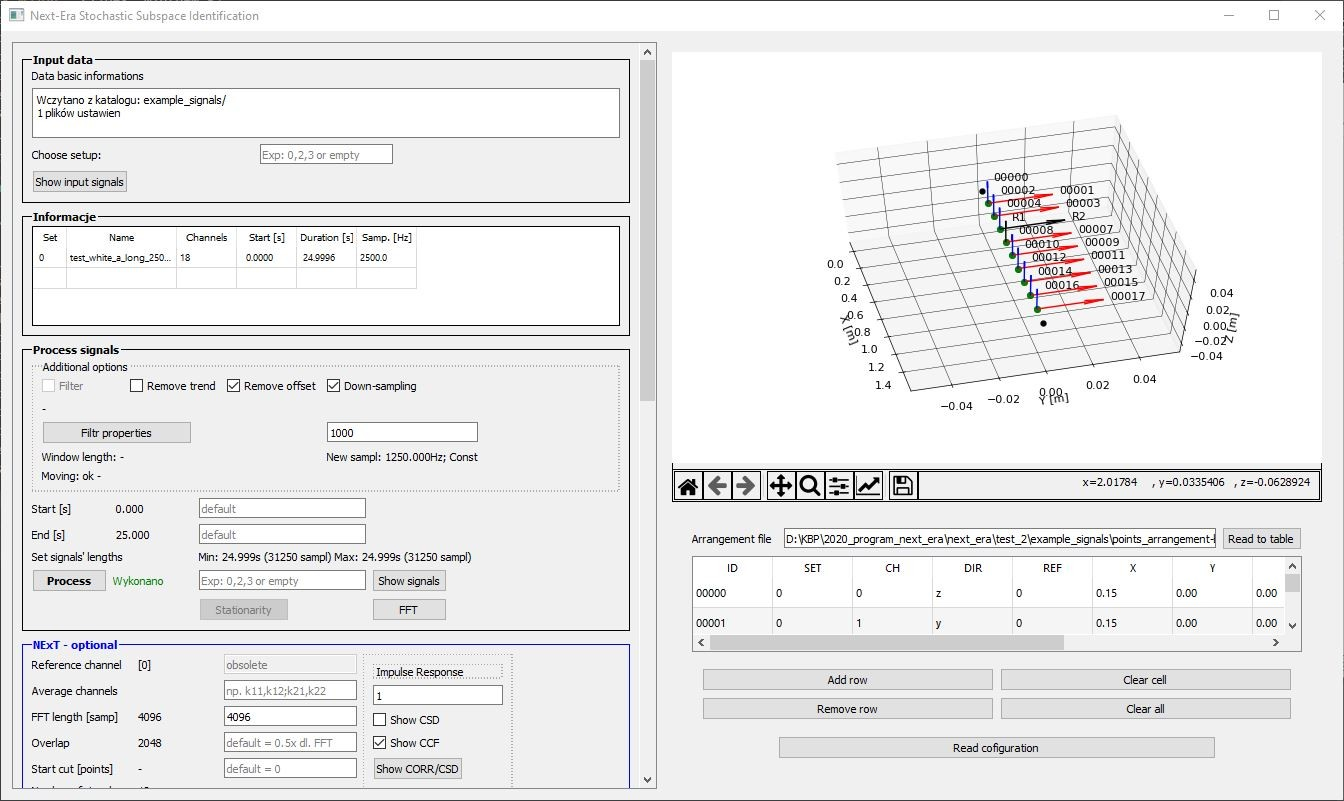
\includegraphics[width=\linewidth]{/program/okno_programu.JPG}
	\captionsetup{justification=centering}
	\caption{Widok na okno główne stworzonej aplikacji do identyfikacji modalnej}
	\label{fig: okno_programu_widok}
\end{figure}

\subsection{Algorytm programu}

Algorytm programu przedstawiono na grafice [].
Poniżej omówiono podstawowe informacje na temat użytych metod przetwarzania sygnałów.

Wstępnie sygnały wyjściowe mogą być poddane standardowemu przetwarzaniu sygnału. Do zastosowanych metod należy filtrowanie, usuwanie składowej stałej i obniżenie próbkowania \teng{downsampling, resampling}. Filtrowanie może posłużyć do odrzucenia niechcianych składowych z sygnału i ograniczyć identyfikację jedynie do określonego obszaru. Odcięcie składowej stałej jest koniecznym elementem przygotowania sygnałów do identyfikacji. Bez tego zabiegu, tak jak w przypadku Transformaty Fouriera występuje istotny pik na zerowej odciętej, tak utrudniona może być identyfikacja modów o niskiej częstotliwości. Zmiana częstotliwości próbkowania jest bardzo przydatną funkcją. Podobnie do filtrowania zmniejsza zakres analizowanej dziedziny, ale w odróżnieniu do filtrowania zmniejsza również liczbę próbek sygnału. Należy pamiętać, że resampling nie jest tożsamy pominięciu części próbek z sygnału. Wpływ obróbki sygnału na wyniki identyfikacji oraz zalecenia dotyczące przyjmowanych parametrów opisał \cite{Caicedo2011} 


Pierwszym głównym etapem w algorytmie NExT-ERA jest wyznaczenie funkcji korelacji wprowadzonych sygnałów. Wyznaczanie funkcji korelacji metodą bezpośrednią jest wymagające obliczeniowo. Z tego powodu wykorzystuje się zależność pomiędzy gęstością widmową mocy, a funkcją korelacji (\ref{eq: spectralDensity} i \ref{eq: correlationInversSpectralDensity}). Wyznaczenie gęstości widmowej mocy jest możliwe za pomocą znacznie bardziej efektywnych algorytmów. Jednym z nich jest metoda Welch'a \parencite{Welch1967,Brincker2015}, którą zastosowano w programie. Umożliwiono również łączenie i uśrednianie wielu serii pomiarowych w jeden wynik identyfikacji. Wykorzystano do tego algorytm przedstawiony w \cite{Brownjohn2010}. W przypadku łączenia serii pomiarowych w jeden wynik, konieczne jest zastosowanie punktów referencyjnych. Punkty referencyjne są to punkty stałe w trakcie całych pomiarów, muszą występować w każdej serii pomiarowej i nie mogą znajdować się w węźle żadnej postaci drgań. Innymi słowy punkt referencyjny musi mieć niezerową wartość w wektorze określającym postać drgań, którą należy zidentyfikować. W zastosowanym algorytmie istnieje możliwość wyboru po jednym punkcie referencyjnym dla każdego z kierunków drgań: X, Y, Z. Łączenie serii pomiarowych odbywa się w następujący sposób:
\begin{itemize}
	\item Algorytmem Welch'a wyznaczane są funkcje wzajemnych gęstości widmowych mocy pomiędzy sygnałem referencyjnym, a pozostałymi sygnałami na powiązanym kierunku.  Wzajemne gęstości widmowe związane z danym punktem referencyjnym są zestawione w jeden wektor.
	\item Wyznaczane są funkcje auto gęstości widmowych mocy dla sygnałów w punktach referencyjnych. Użyty jest do tego ten sam algorytm co w przypadku wzajemnych funkcji gęstości widmowej mocy, z tą różnicą że sygnały wejściowe są identyczne. 
	\item Funkcje wzajemnej gęstości widmowej mocy zestawione w jednym wektorze dzielone są przez funkcję auto gęstości widmowej punktu referencyjnego. W tym przypadku wymagane jest aby długość wektora wszystkich wektorów była równa. Identycznie postępuje się z każdym wektorem gęstości widmowych mocy.
	\item Auto gęstości widmowe mocy dla danego punktu referencyjnego są uśredniane. Auto gęstości widmowe mocy są sumowane ze wszystkich ustawień, a wynik jest podzielony przez liczbę ustawień.
	\item Po procesie uśredniania gęstości widmowych mocy punktów referencyjnych następuje działanie odwrotne. Wcześniej podzielone wzajemne gęstości widmowe mocy mnożone są przez uśrednione auto gęstości widmowe mocy punktów referencyjnych.
	\item Wynikowe gęstości widmowe mocy przekształcane są za pomocą odwrotnej Transformaty Fouriera do sygnałów w dziedzinie czasu. Otrzymany wynik odpowiada funkcjom cross-korelacji i może być użyty w metodzie ERA.
	
\end{itemize}

Uśrednianie serii pomiarowych z tym samym ustawieniem punktów pomiarowych odbywa się przez sumowanie gęstości widmowych mocy z powtórzonych serii pomiarowych i podzieleniu przez liczbę powtórzonych serii. Pomimo zestawienia funkcji gęstości widmowych mocy w wektory, wszystkie wspomniane wyżej operacje mnożenia i dzielenia funkcji gęstości widmowych mocy polegają na działaniu na poszczególne prążki spektrum, a nie na klasycznym rozumieniu mnożenia i dzielenia wektorów. 

\subsection{Elementy oceny poprawności rozwiązania}
Ważnym elementem w procesie identyfikacji modalnej jest ocena poprawności uzyskanego rozwiązania. W tym celu najczęściej wykorzystywane są diagramy stabilizacyjne. W przypadku pomiarów obarczonych szumem, przyjęty rząd modelu musi być zadeklarowany jako większy niż miało by to miejsce w idealnych warunkach. Diagram stabilizacyjny pozwala na określenie minimalnego rzędu modelu, przy którym występują wszystkie interesujące mody i są one stabilne. Zastosowanie diagramów stabilizacyjnych opisano między innymi w (!!!). W programie zastosowano dwie wersje diagramów: niefiltrowaną i filtrowaną. Wersja niefiltrowana obrazuje wszystkie wyznaczone mody: rzeczywiste i fikcyjne. Odróżnia je w zależności od wyników dla niższego rzędu modelu. Jeśli istnieje w modelu o rząd niższym mod spełniający odpowiednie kryteria to jest on uznany za rzeczywisty. Dla rzędu modelu $n$ i obliczonego modu $i$ zastosowane w programie domyślne kryteria to:
\begin{itemize}
	\item częstotliwość $f$ w dwóch kolejnych krokach nie może się różnić o więcej niż 1\%,
	\begin{equation}\label{eq: stabdiag_crit_freq}
		\Delta f =  \Big| 1-\frac{f_{n,i}}{f_{n+1,i}}\Big|  \le 0.01
	\end{equation}
	\item tłumienie $\xi$ w dwóch kolejnych krokach nie może się różnić o więcej niż 5\%,
		\begin{equation}\label{eq: stabdiag_crit_ksi}
		\Delta \xi =  \Big| 1-\frac{\xi_{n,i}}{\xi_{n+1,i}}\Big|  \le 0.05
	\end{equation}
	\item parametr MAC dla postaci w dwóch kolejnych krokach musi być większy niż 0.95,	
	\item parametr MPC postaci modu musi być większy niż 0.9.
	\begin{equation}\label{eq: stabdiag_crit_MPC_MAC}
		\text{MAC}_i^{n,n+1} \ge 0.95 \qquad \text{MPC}_i \ge 0.90
	\end{equation}
\end{itemize}
Diagram niefiltrowany obrazuje rozkład zidentyfikowanych modów w domenie częstotliwości. Wstępnie pozwala ocenić czy istnieją mody stabilne (częstotliwość i tłumienie), o rzeczywistych wektorach postaci (MPC) i o niezmiennej formie (MAC). W przypadku dużego rzędu modelu i bliskich sobie modów trudno jednoznacznie odnaleźć jedynie poprawne rozwiązania. Z tego względu stworzono również wersję filtrowaną diagramu stabilizacyjnego. Diagram filtrowany w znacznie bardziej czytelny sposób pozwala przedstawić jedynie mody uznane za rzeczywiste. Jego generacja opiera się na następujących krokach:
\begin{itemize}
	\item Podział dziedziny częstotliwości na wąskie pasma (np. 1\% dolnej granicy pasma) i podział wszystkich punktów według przynależności do poszczególnych pasm,
	\item Odrzucenie punktów, dla których tłumienie jest zbyt duże ($\text{LDT}\ge0.3$) lub ujemne,
	\item Wyznaczenie parametru MAC pomiędzy wszystkimi punktami w paśmie oraz parametru MPC dla każdego modu w paśmie.
	\item Wyznaczenie wartości średniej i odchylenia standardowego częstotliwości, tłumienia i parametrów MAC i MPC dla punktów pasma. Jeżeli wartości średnie pomniejszone o odchylenie standardowe są spełniają dopuszczalne warunki, to zestaw punktów uznany jest za określający rzeczywisty mod. Jeżeli nie, wyszukiwany jest punkt charakteryzujący się najgorszym parametrem MAC lub MPC albo zbyt różniącą się liczbą tłumienia i jest odrzucany. Następnie ponownie oceniana jest wartość średnia i odchylenie standardowe. Proces ten toczy się do momentu odrzucenia wszystkich punktów lub spełnienia kryteriów uznania mod za rzeczywisty.
	\item Ostatecznie jako rzeczywiste i stabilne określane są mody, dla których liczba punktów w paśmie jest większa od wartości minimalnej. Domyślnie jest to 20\% maksymalnego rzędu modelu na diagramie.
\end{itemize}
Wskaźniki MAC i MPC są istotną częścią algorytmu programu i służą ocenie poprawności wyników. Poniżej przytoczono ich definicje i podstawowe właściwości. 

\subsubsection{Model Phase Colinearity (MPC)}
Wynikiem przeprowadzonej analizy modalnej są postaci i częstotliwości o wartościach zespolonych. Postaci zidentyfikowane na podstawie pomiarów wartości rzeczywistych powinny stanowić wektory o współrzędnych rzeczywistych. W przypadku modów normalnych wszystkie punkty konstrukcji drgają dokładnie w fazie lub w przeciw fazie względem siebie. Przeciwnie, kiedy postaci są wektorami zespolonymi, przemieszczenia osiągają wartości ekstremalne w różnych chwilach czasowych dla różnych stopni swobody. \cite{Ewins2000,Chopra2012a} podają przykładowe przyczyny powstania postaci o wektorach zespolonych. Są to m.in. efekt żyroskopowy, efekty aerodynamiczne, nieliniowość czy nieproporcjonalne tłumienie. Zidentyfikowane mody zwykle występują w postaci zespolonej. Wynika to z relatywnie niskiego wskaźnika sygnału do szumu \parencite{Rainieri2014}. Mimo to, "stopień zespolenia" jest zwykle niewielki i w praktycznych zastosowaniach błąd wynikający z tej cechy może być zaniedbany. Mimo to ważnym jest żeby rozróżnić, które mody są normalne, a które w dużej mierze zespolone. Jedną z najprostszych metod jest wykreślenie współrzędnych składników postaci w układzie biegunowym. Metoda została szerzej opisana w \parencite{Ewins2000}. Zasadą jest, że jeśli w konstrukcji występuje tłumienie proporcjonalne to składniki danej postaci układają się na linii prostej w zespolonym układzie współrzędnych \parencite{Rainieri2014}).
Do ilościowego określenia stopnia przestrzennej spójności modu \cite{Pappa1992} opracowali wskaźnik MPC (\textit{Modal Phase Collinearity}). Jest on dla $i$-tego moda określony wzorem \ref{eq:mpc_ratio}
\begin{equation}
	{S}_{xx}={\mathbf{\Phi}'}_{i}^{\mathsf{T}} {\mathbf{\Phi}} '_{i} \quad
	%\end{equation}
	%\begin{equation}
	{S}_{yy}={\mathbf{\Phi}''}_{i}^{\mathsf{T}} {\mathbf{\Phi}}''_{i} \quad
	%\end{equation}
	%\begin{equation}
	{S}_{xy}={\mathbf{\Phi}'}_{i}^{\mathsf{T}} {\mathbf{\Phi}}''_{i}
\end{equation}
\begin{equation}
	{\mu}=\frac{S_{xx}-S_{yy}}{2S_{xy}} \quad \quad
	\beta=\mu+\mathrm{sgn}(S_{xy})\sqrt{\mu^{2}+1} \quad \quad
	\tau=\tan^{-1}{(\beta)} \quad
\end{equation}
\begin{equation}
	\lambda_{1}=S_{xx}+\frac{S_{xy}(2(\mu^{2}+1)\sin^{2}{(\tau)}-1)}{\mu}
\end{equation}
\begin{equation}
	\lambda_{2}=S_{yy}+\frac{S_{xy}(2(\mu^{2}+1)\sin^{2}{(\tau)}-1)}{\mu}
\end{equation}
\begin{equation} \label{eq:mpc_ratio}
	\mathrm{MPC}_{i}=\left[2\cdot\left(\frac{\lambda_{1}}{\lambda_{1}+\lambda_{2}}-0.5\right)\right]^{2}
\end{equation}
gdzie $\mathrm{sgn}(\cdot)$ oznacza funkcję zwracającą znak liczby. Wskaźnik MPC jest bezwymiarowy i przyjmuje wartości z zakresu od 0 (dla modów z zupełnie nieskorelowanymi kątami fazowymi) do 1 (dla modów jednofazowych).
\subsubsection{Modal Assurance Criterion (MAC)}

Kryterium MAC (Modal Assurance Criterion) pozwala ocenić miarę dopasowania (stopień liniowości) dwóch wektorów modalnych \parencite{Allemang1982}. Jest to podstawowe i najbardziej popularne kryterium służące porównaniu wektorów modalnych \cite{Rainieri2014}. Jego wartość waha się od 0 (dla braku dopasowania) do 1 (dla idealnego dopasowania). Definicja wskaźnika dana jest wzorem \ref{eq: MAC_definition}.
\begin{equation} \label{eq: MAC_definition}
	\text{MAC}_n = \frac{ (\vect{\psi_{n,a}}^H\vect{\psi_{n,e}})^2}
	{\vect{\psi_{n,a}}^H\vect{\psi_{n,a}}\vect{\psi_{n,e}}^H\vect{\psi_{n,e}}}
\end{equation}
gdzie $\vect{\psi_{n,a}}$ i $\vect{\psi_{n,e}}$ to wektory postaci drgań własnych, a $(\cdot)^H$ oznacza sprzężenie Hermitowskie wektora.
Należy pamiętać, że kryterium MAC nie wskazuje czy rozwiązanie jest poprawne lub czy wektory modalne są ortogonalne. Wynik pokazuje jedynie dopasowanie dwóch wektorów. Wskaźnik MAC jest nieodporny na błędy zawarte jednocześnie w obu wektorach. Z tego względu za każdym razem należy kontrolować założenia metody. Zbiór wskazówek do stosowania kryterium MAC w swojej pracy zawarł \cite{Allemang2003}. Poza swoistą instrukcją użycia wskaźnika, wskazuje on następujące główne przyczyny niemiarodajnych wyników przy korzystaniu z kryterium MAC:
\begin{itemize}[noitemsep]
	\item traktowanie kryterium MAC jako informacji o ortogonalności wektorów,
	\item nieprawidłowe matematyczne sformułowanie kryterium, głównie zastąpienie sprzężenia Hermitowskiego transpozycją. Zmiana ta jest słuszna wyłącznie przy rzeczywistych wektorach modalnych,
	\item duże różnice w wartościach współrzędnych wektorów. Kryterium jest bardzo wrażliwe na duże wartości, a niewrażliwe na małe wartości,
	\item przyjęcie zbyt małej liczby współrzędnych wektora,
	\item wypełnienie zerami współrzędnych wektora, na temat których nie ma żadnej informacji.
\end{itemize}

Ze względu na ograniczenia kryterium MAC, od momentu jego powstania powstał szereg pokrewnych wskaźników. Są to między innymi: Coordinate Modal Assurance Criterion (COMAC) \parencite{Ewins2000}, Enhanced Coordinate Modal Assurance Criterion (ECOMAC) \parencite{Hunt1992} czy Inverse Modal Assurance Criterion (IMAC) \parencite{MITCHELL1998}. Każde z kryteriów zostało zmodyfikowane w celu wyeliminowania konkretnego ograniczenia oryginalnej wersji. Zestawienie i opis wielu z nich przedstawiono miedzy innymi w pracach \parencite{Allemang2003,Rainieri2014,Szafranski2013,Salamak2003} 

Poza diagramem stabilizacyjnym, w niniejszej pracy kryterium MAC zostało również użyte przy doborze lokalizacji czujników w trakcie pomiarów na konstrukcji rzeczywistej. Jest to kolejne z popularnych zastosowań współczynnika MAC \parencite{Allemang2003}. Polega na takim doborze punktów pomiarowych, aby zidentyfikowane w tych punktach postaci drgań były od siebie maksymalnie różne. Opis przyjętego rozwiązania i wyniki obliczeń przedstawiono w wynikach badań w rozdziale \ref{sect: identyfikacja_modalna_wk2}.




\subsection{Testy numeryczne metody NEXT-ERA}
Każda aplikacja komputerowa przed użyciem powinna być poddana testom. W przypadku aplikacji służącej celom naukowym, gdzie zakłada się pewien poziom wiedzy i świadomości użytkownika zdecydowano, że testom poddane zostanie jedynie jądro programu - algorytm NExT-ERA. W tym celu założono wykonanie dwóch testów: numerycznego i laboratoryjnego. Test numeryczny ma opierać się na wykonaniu modelu obliczeniowego w oprogramowaniu MES, a następnie obciążeniu go losowo (w przybliżeniu szumem białym) i wykonaniu analizy dynamicznej. Test laboratoryjny ma polegać na pomiarze i analizie drgań środowiskowych rzeczywistego obiektu badawczego. Celem testu nie jest uzyskanie idealnej zgodności pomiędzy wynikami z badania numerycznego i laboratoryjnego, a jedynie sprawdzenie działania programu. Wyniki uzyskane z testu numerycznego są pozbawione wpływu wielu niedokładności, takich jak szumów, nieliniowych warunków brzegowych, nieosiowo ustawionych czujników czy wzajemnego wpływu składowych ortogonalnych na mierzone wartości. Dlatego traktowane są głównie jako test algorytmu. Mogą również służyć jako punkt odniesienia do wyników badań laboratoryjnych. Z kolei badania laboratoryjne pozwolą sprawdzić czy program i system pomiarowy są odporne na rzeczywiście występujące obciążenia procesu identyfikacji.

Przedmiotem badań była konstrukcja o schemacie statycznym bliskim belce swobodnie podpartej. Głównym elementem układu jest kształtownik stalowy o przekroju ceowym C40 i o długości 1.5m. Obiekt został opisany szerzej w punkcie \ref{sect: next_era_lab_test}).  Model numeryczny wykonano w programie MES bazujac na inwentaryzacji wymiarów obiektu laboratoryjnego. Założono, że głównym aspektem porównawczym z badaniami laboratoryjnymi mają być mody giętne pionowe. Z tego powodu znacznie uproszczono względem rzeczywistości strefy podporowe. Nie wykonano żadnej kalibracji modelu, aby odpowiadał lepiej strukturze rzeczywistej. Do budowy wykorzystano środowisku MES SOFiSTiK. Dla odwzorowania całego układu użyto jednowymiarowych elementów belkowych. Wizualizację oraz schemat statyczny pokazano na rysunku \ref{fig: test_beam_wis_model}.
\begin{figure}[h]
	\centering
	\subfloat[Wizualizacja]{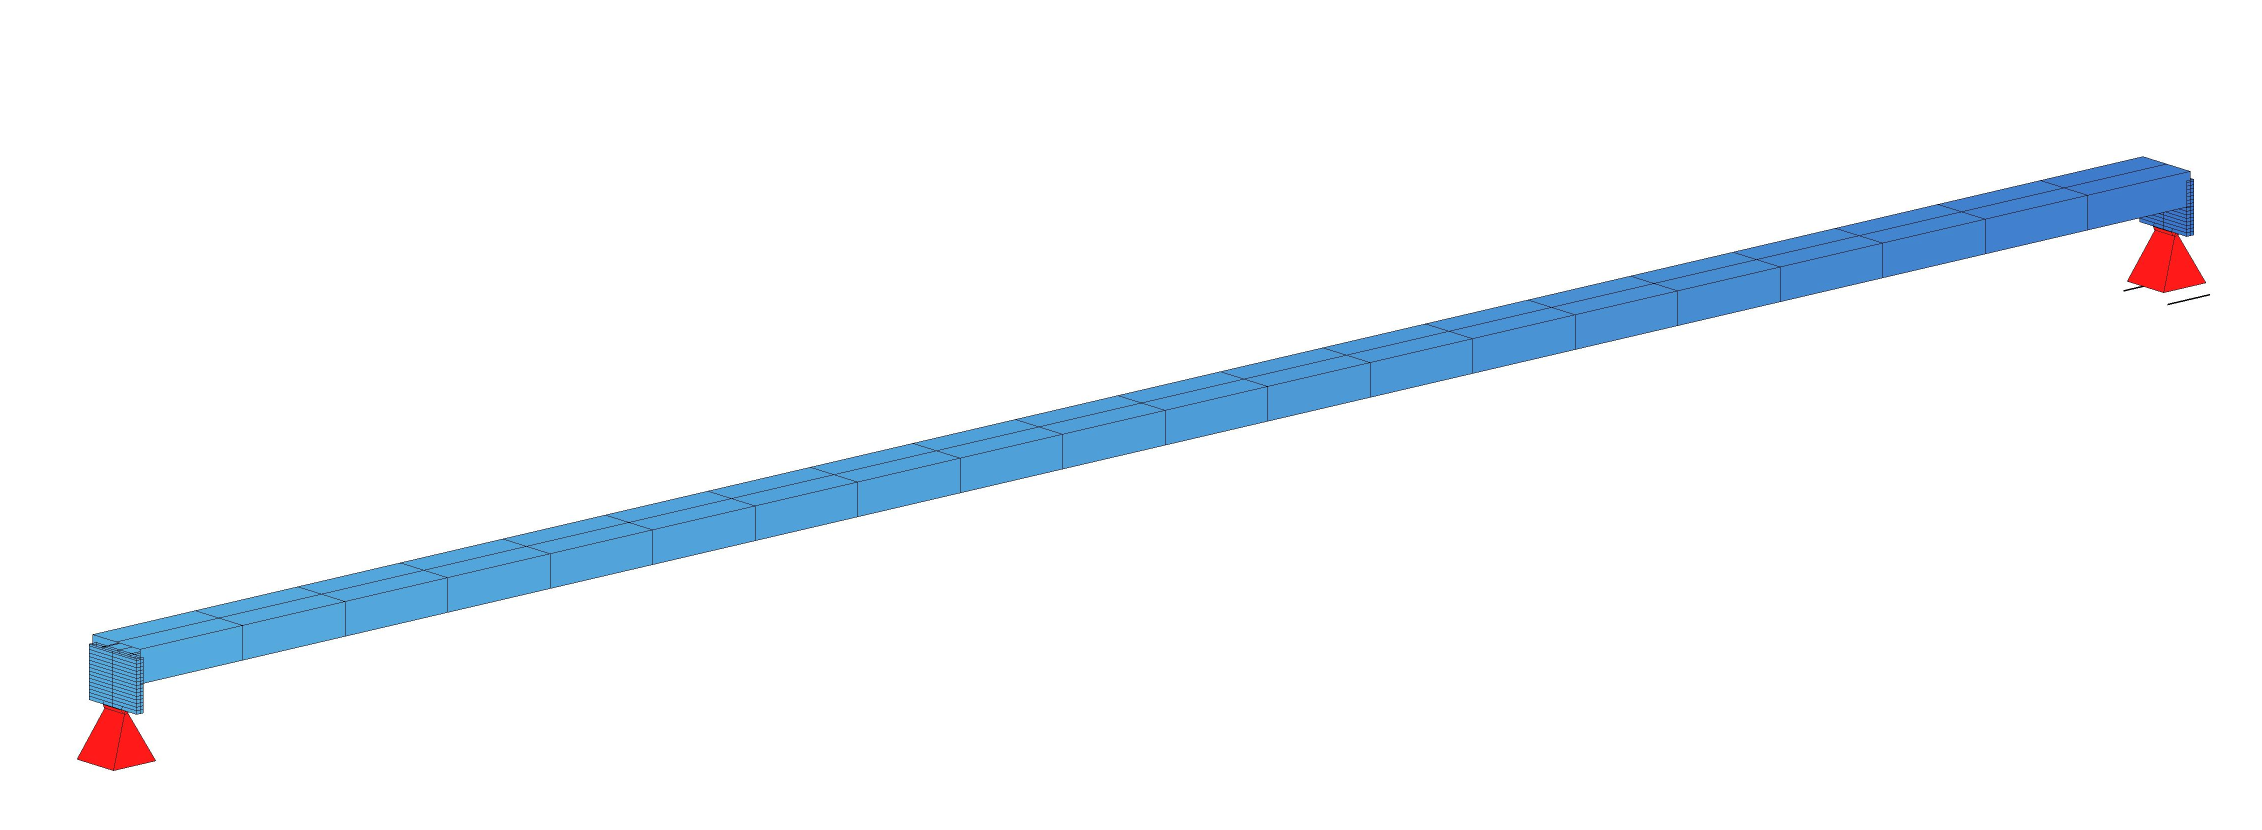
\includegraphics[width=0.5\linewidth]{/test_blue/sof_wis/wis_small002.png}}%
	\subfloat[Schemat statyczny]{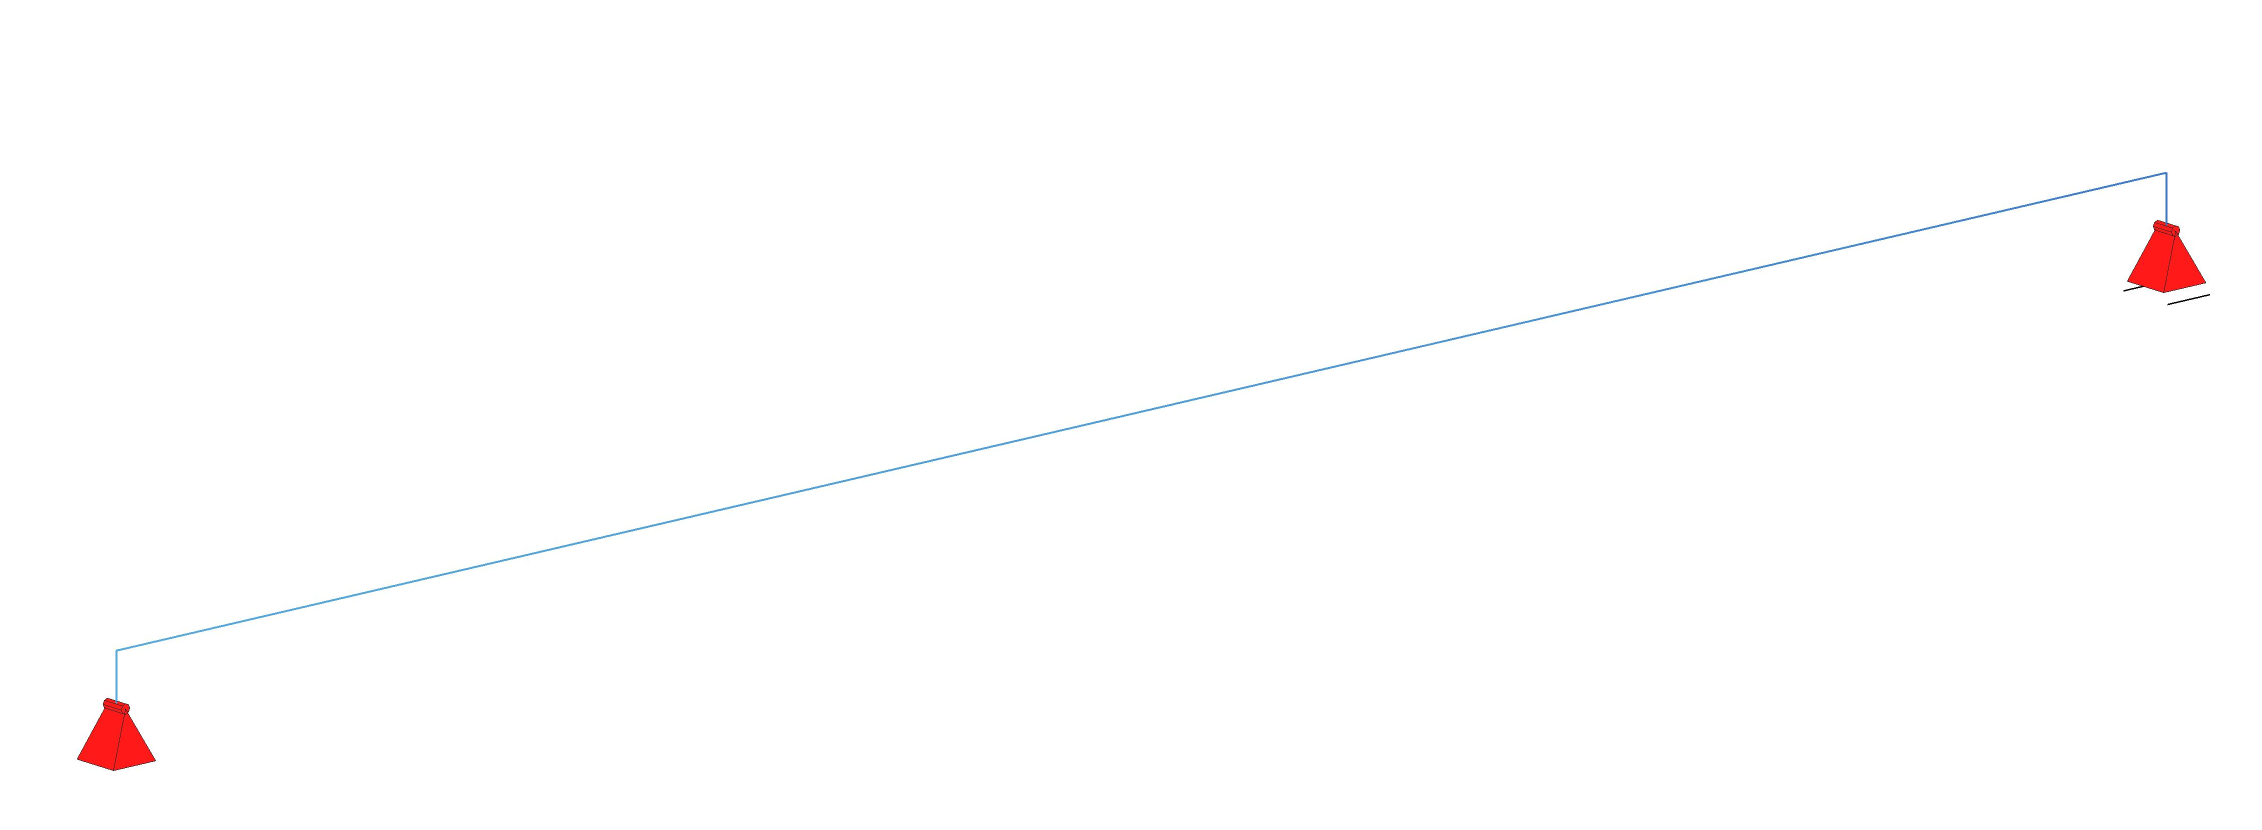
\includegraphics[width=0.5\linewidth]{/test_blue/sof_wis/wis_small001.png}}%
	\captionsetup{justification=centering}
	\caption{Wizualizacja i schemat statyczny testowego modelu numerycznego}
	\label{fig: test_beam_wis_model}
\end{figure}




Przed przystąpieniem do analizy wygenerowano 5000 losowych przypadków obciążenia. Losowy charakter uzyskano za pomocą następujących założeń dla każdego przypadku obciążenia:
\begin{itemize}
	\item w każdym węźle pośrednim może, ale nie musi, być przyłożona siła pionowa lub poprzeczna,
	\item jeśli siła została przyłożona, jej wartość jest losowana z zakresu od -3 do 3 N dla każdego węzła indywidualnie,
	\item w trakcie analizy, w każdym kroku czasowym losowany jest jeden przypadek obciążenia z wygenerowanych 5000.
\end{itemize}
Rozwiązano problem własny dynamiki przedmiotowego modelu i otrzymano rezultaty jak na rysunku \ref{fig: modal_mods_blue_beam}.

\begin{figure}[h]
	\centering
	\subfloat[Mod 1, $f_1=19.70 \text{Hz}$]{\label{fig: test_blue_sof_mod1}%
		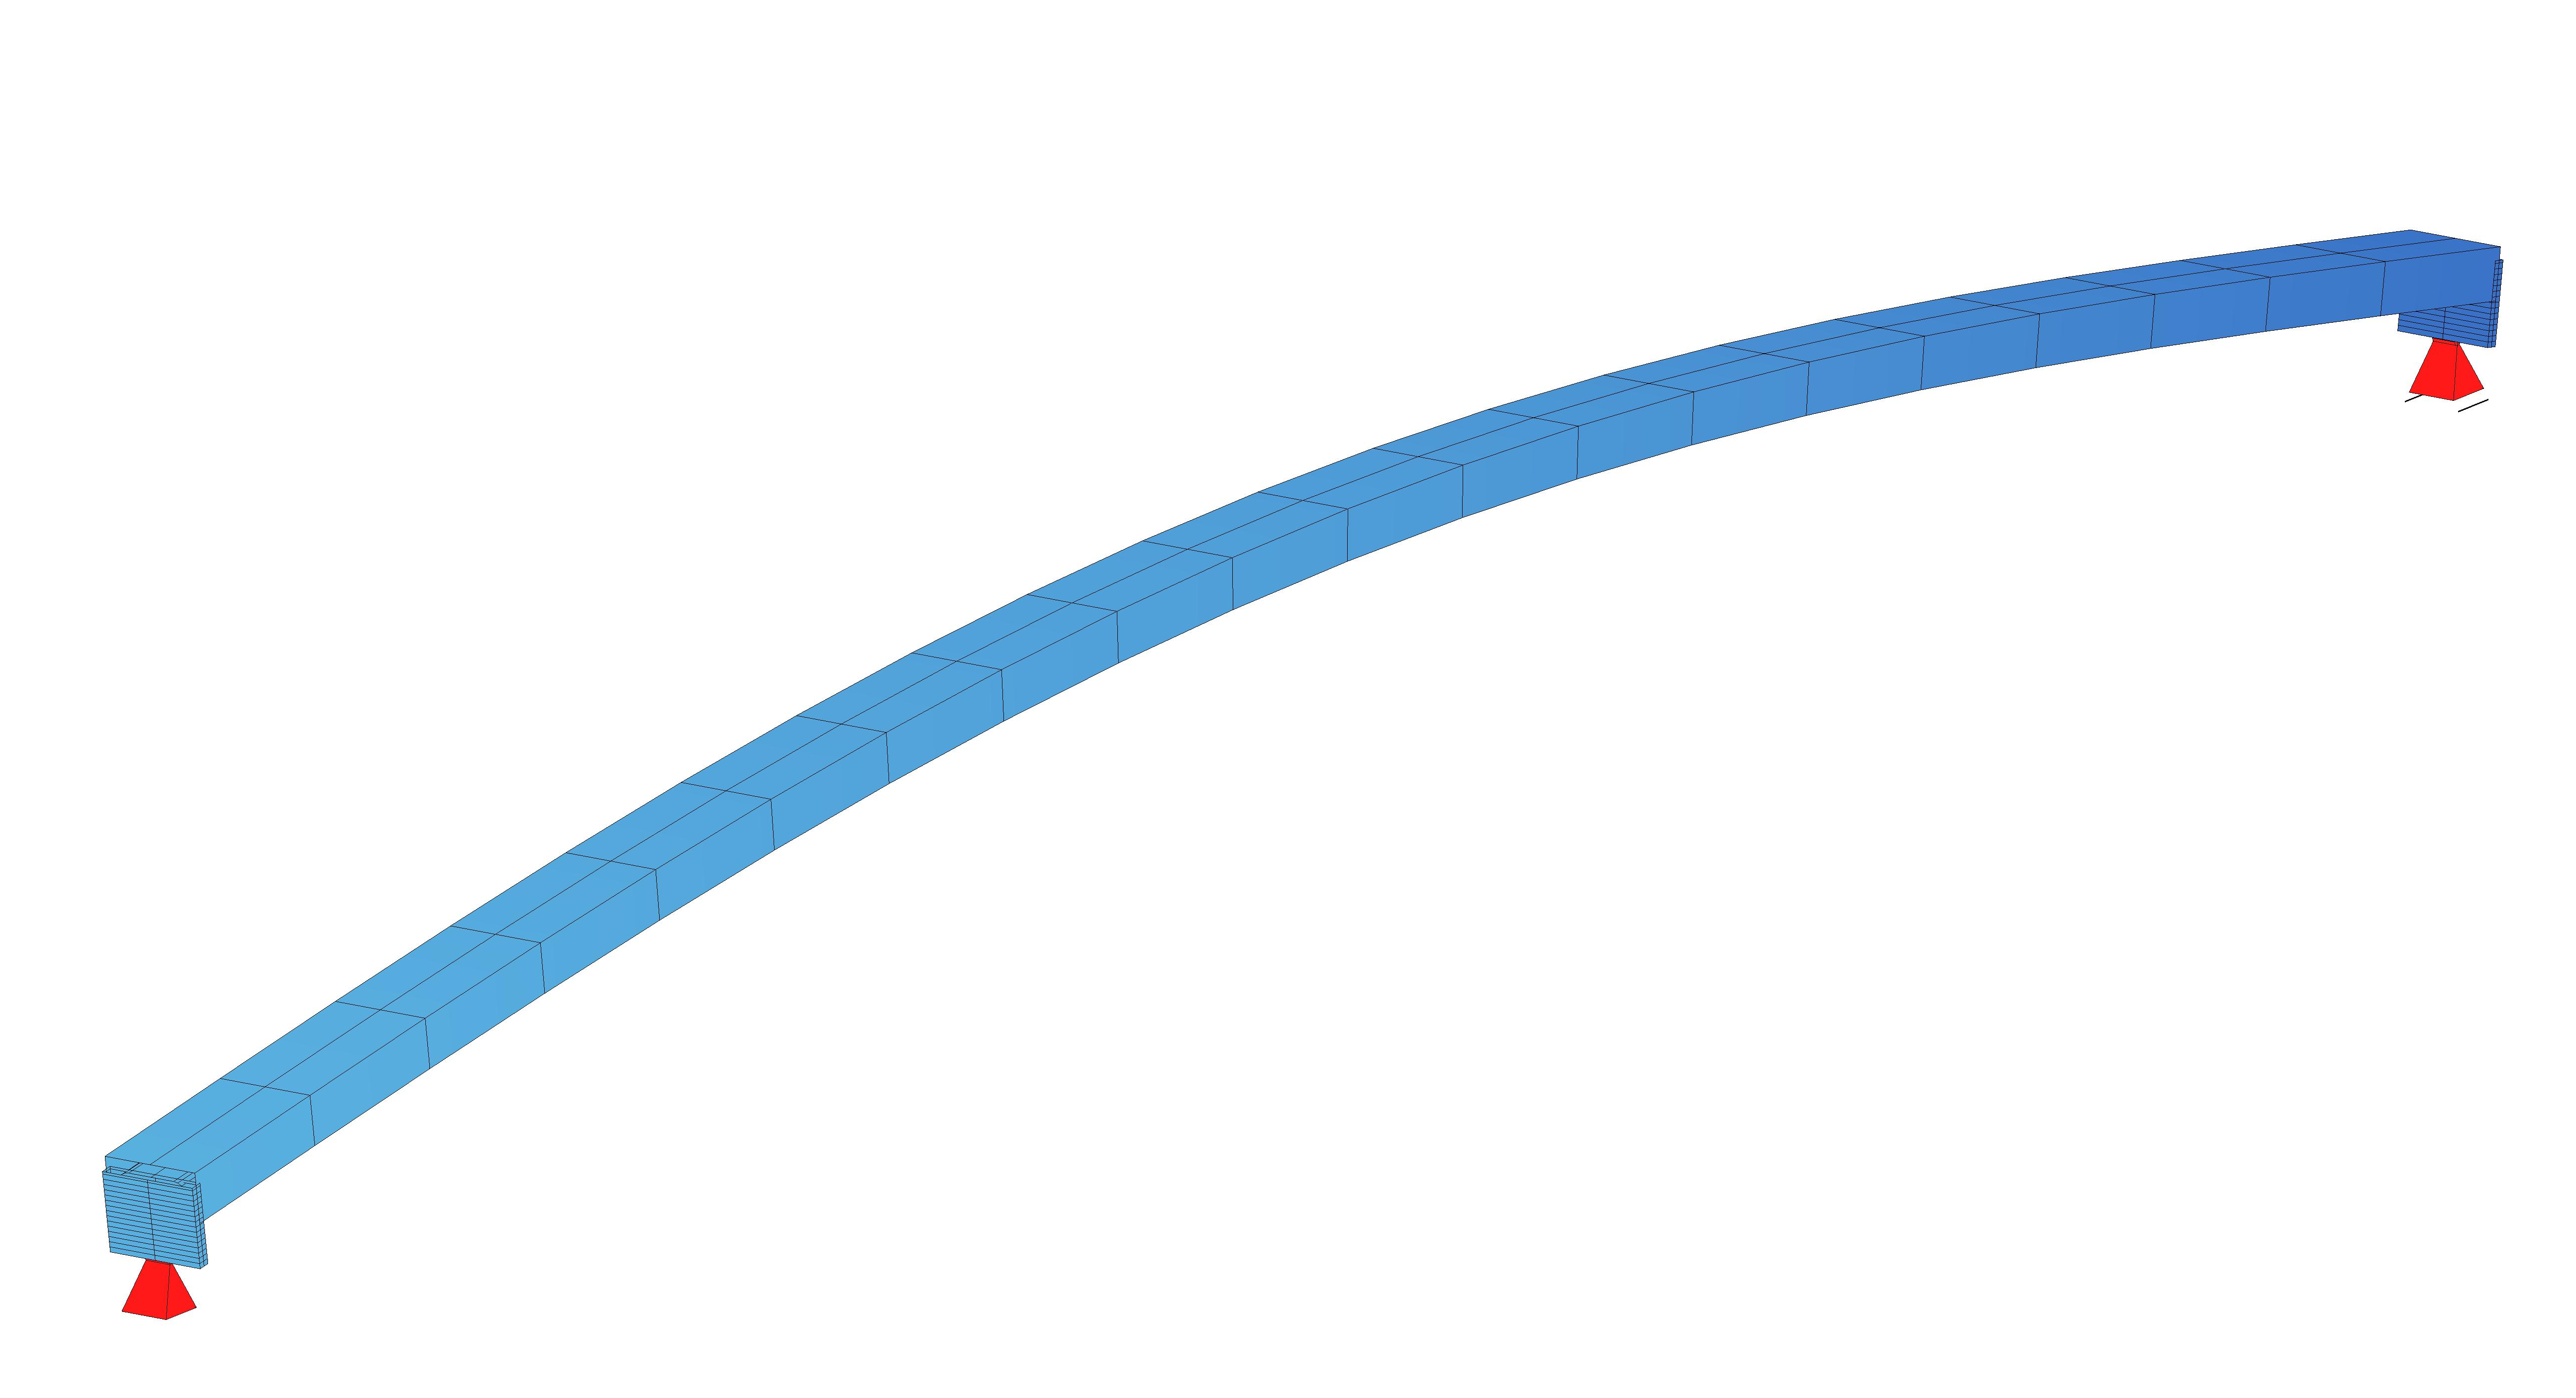
\includegraphics[width=0.33\linewidth]{/test_blue/sof_wis/image_small001.png}}%
	\subfloat[Mod 2, $f_2=54.93 \text{Hz}$]{\label{fig: test_blue_sof_mod2}%
		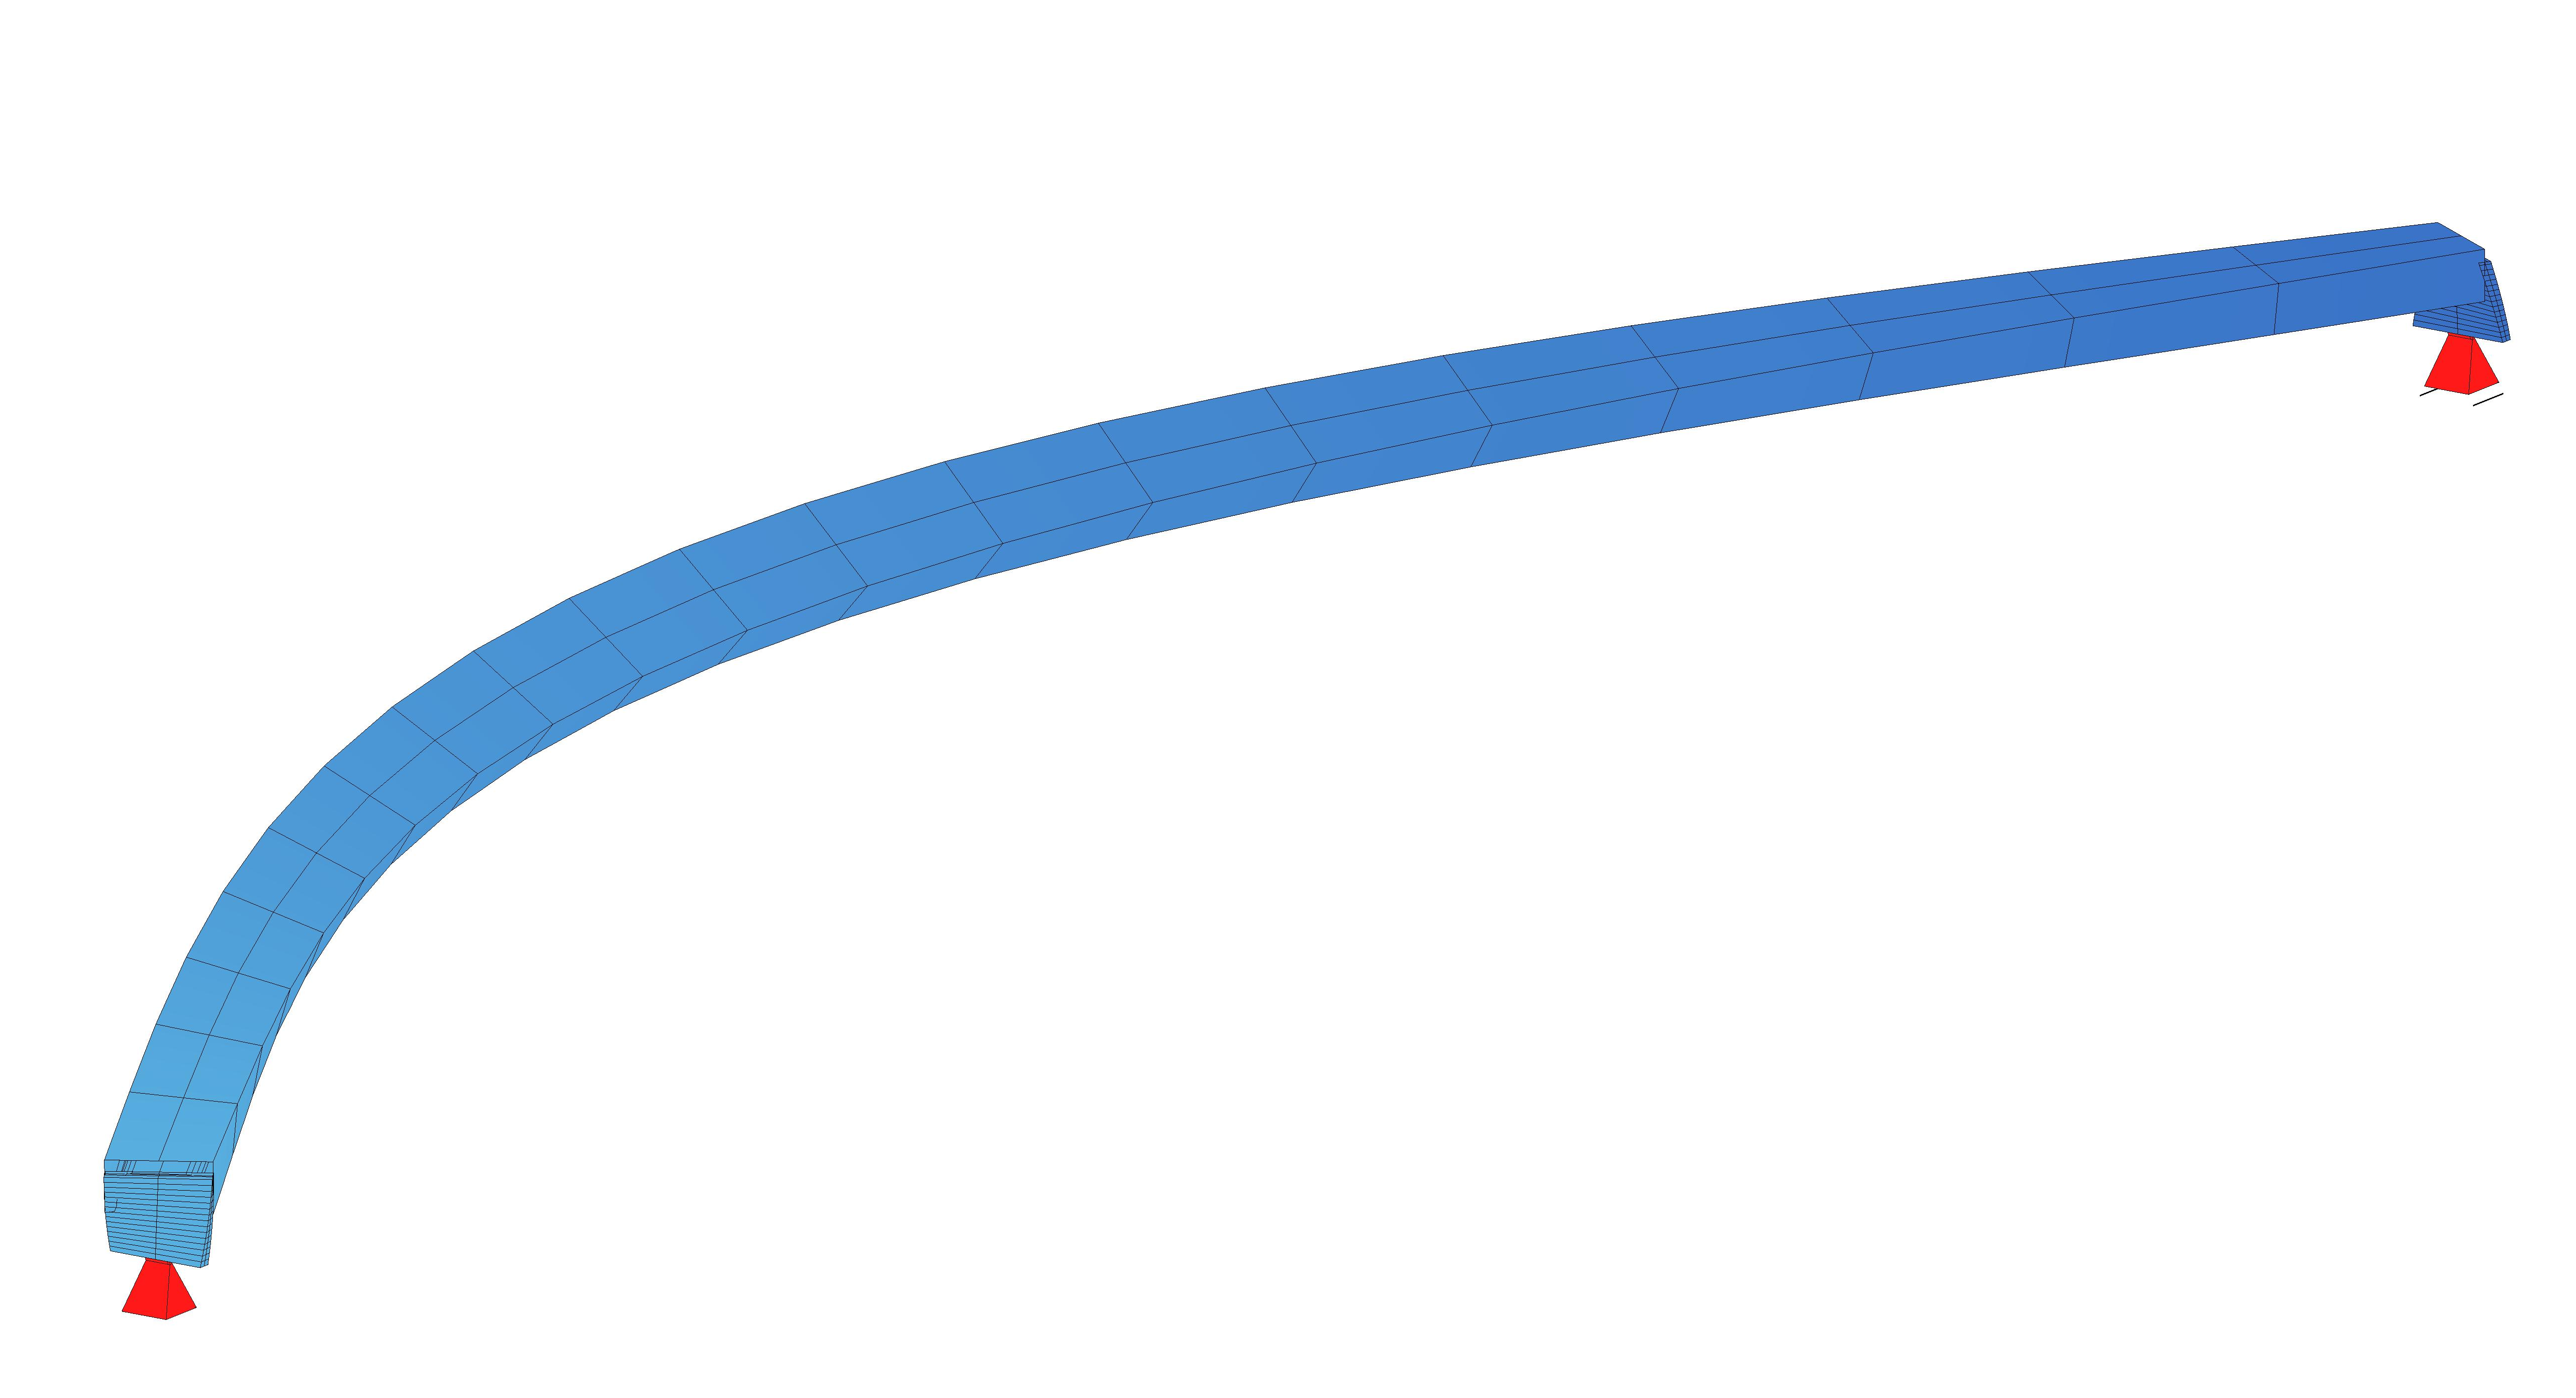
\includegraphics[width=0.33\linewidth]{/test_blue/sof_wis/image_small003.png}}%	
	\subfloat[Mod 3, $f_3=78.20 \text{Hz}$]{\label{fig: test_blue_sof_mod3}%
		\includegraphics[width=0.33\linewidth]{/test_blue/sof_wis/image_small004.png}}\\		
	\subfloat[Mod 4, $f_4=161.35 \text{Hz}$]{\label{fig: test_blue_sof_mod4}%
		\includegraphics[width=0.33\linewidth]{/test_blue/sof_wis/image_small005.png}}%
	\subfloat[Mod 5, $f_5=200.38 \text{Hz}$]{\label{fig: test_blue_sof_mod5}%
		\includegraphics[width=0.33\linewidth]{/test_blue/sof_wis/image_small006.png}}%
	\subfloat[Mod 6, $f_6=212.24 \text{Hz}$]{\label{fig: test_blue_sof_mod6}%
		\includegraphics[width=0.33\linewidth]{/test_blue/sof_wis/image_small007.png}}\\
	\subfloat[Mod 7, $f_7=217.12 \text{Hz}$]{\label{fig: test_blue_sof_mod7}%
		\includegraphics[width=0.33\linewidth]{/test_blue/sof_wis/image_small008.png}}%
	\subfloat[Mod 8, $f_8=336.59 \text{Hz}$]{\label{fig: test_blue_sof_mod8}%
		\includegraphics[width=0.33\linewidth]{/test_blue/sof_wis/image_small009.png}}%
	\subfloat[Mod 9, $f_9=410.22 \text{Hz}$]{\label{fig: test_blue_sof_mod9}%
		\includegraphics[width=0.33\linewidth]{/test_blue/sof_wis/image_small010.png}}\\
	\subfloat[Mod 10, $f_{10}=451.89 \text{Hz}$]{\label{fig: test_blue_sof_mod10}%
		\includegraphics[width=0.33\linewidth]{/test_blue/sof_wis/image_small011.png}}\\
	
	\caption{Rozwiązanie analizy modalnej modelu testowego}
	\label{fig: modal_mods_blue_beam}
\end{figure}

Odpowiedź konstrukcji na wymuszenie losowe wyznaczono metodą time-step Newmarka-Wilsona. Zdecydowano o sprawdzeniu modów w zakresie do około 250Hz. Z tego względu przyjęto krok całkowania jako $\Delta t = 1/2500 s$. Zgodnie z kryterium Nyquista taki krok pozwala identyfikować drgania teoretycznie do częstotliwości 1250 Hz. Niemniej jednak, sygnał wyjściowy powinien zostać nadpróbkowany znacznie bardziej niżeli dwukrotnie. Aby zapewnić dokładność rezultatu, odpowiedź z rozwiązania numerycznego powinna być wyznaczona z próbkowaniem ok 10-15 razy większym niż częstotliwość najwyższego, interesującego modu \parencite{Kacprzyk1983,Rakowski2016,Bajer2012,Zotowski2017c}. Większość modów odczytanych z analizy modalnej mieści się w zamierzonym zakresie do 250 Hz. Kilka modów powyżej 250 Hz zostanie również uwzględnione w analizie dla pokazania zmniejszenia dokładności z uwagi na zbyt rzadkie próbkowanie. W każdym kroku struktura była obciążana losowym przypadkiem obliczeniowym z bazy 5000 wcześniej wygenerowanych. Tłumienie konstrukcji przyjęto jako masowo-sztywnościowe według metody Rayleigha (\ref{eq: rayleigh_damping}). Współczynniki metody wyznaczono zakładając tłumienie $\text{LDT}=3\%$ dla częstotliwości 20 Hz i 160 Hz. Chcąc sprawdzić charakter obciążenia wykonano analizę FFT sygnału złożonego z wartości obciążenia czterech węzłów w funkcji czasu. Widma częstotliwościowe przedstawiono na rysunku \ref{fig: fft_load_input_blue_beam}. Całkowity czas analizy przyjęto równy 25s ($25\cdot2500=62500$ kroków czasowych). Widmo częstotliwościowe nie ujawnia żadnej dominującej częstotliwości i można uznać je za równe w całym zakresie.
\begin{figure}[h]
	\centering
	\subfloat[Węzeł 7, kierunek Y]{\includegraphics{/test_blue/input_load/input_load_1.pdf}}%
	\subfloat[Węzeł 7, kierunek Z]{\includegraphics{/test_blue/input_load/input_load_2.pdf}}\\
	%\subfloat[Węzeł 11, kierunek Y]{\includegraphics{/test_blue/input_load/input_load_3.pdf}}%
	%\subfloat[Węzeł 11, kierunek Z]{\includegraphics{/test_blue/input_load/input_load_4.pdf}}%
	\captionsetup{justification=centering}
	\caption{Transformaty Fouriera funkcji wymuszenia przykładowych węzłów w modelu testowym}
	\label{fig: fft_load_input_blue_beam}
\end{figure}

Dla obliczonego modelu odczytano przebieg przyspieszeń w dziewięciu węzłach pośrednich, na kierunku pionowym i poprzecznym. Do programu wprowadzono stworzone sygnały z informacją o lokalizacji punktów odczytu. Jako punkt referencyjny na kierunku $Y$ wybrano punkt odległy o 0.3L od podpory, a na kierunku pionowym $Z$ punkt odległy o 0.4L od podpory. O wyborze punktów referencyjnych decyduje warunek, że nie mogą one znajdować się w węzłach żadnej analizowanej postaci drgań. Doboru parametrów identyfikacji dokonano przy pomocy diagramu stabilizacyjnego (Rys. \ref{fig: stab_diags_blue_beam}). Na ostatecznym diagramie w wersji filtrowanej (Rys. \ref{fig: stab_diags_blue_beam_b}) wyraźnie widać 8 zidentyfikowanych, stabilnych modów. Odczytano minimalny rząd modelu zawierający wszystkie stabilne mody jako $n=20$. Diagram tworzony iteracyjnie pozwolił ostatecznie wyznaczyć parametry metody, które przynoszą pewne, stabilne rozwiązanie. Dobrane parametry użyto w celu wyznaczenia ostatecznego rozwiązania identyfikacji.

\begin{figure}[ht]
	\centering
	\subfloat[Diagram niefiltrowany]{\includegraphics[width=\linewidth]{/test_blue/stab_diag/fig_stab_diagram_nonfiltr_time_20_20_50.pdf}}\\
	\subfloat[Diagram filtrowany]{\includegraphics[width=\linewidth]{/test_blue/stab_diag/fig_stab_diagram_filtr_time_20_20_54.pdf},\label{fig: stab_diags_blue_beam_b}}%
	\captionsetup{justification=centering}
	\caption{Diagram stabilizacyjny metody NExT-ERA testowego modelu numerycznego: (a) diagram niefiltrowany, (b) diagram filtrowany}
	\label{fig: stab_diags_blue_beam}
\end{figure}

Wprowadzono wyznaczone parametry do programu. Uzyskano odpowiedzi impulsowe dla każdego punktu, których przykłady wraz z odpowiadającą im transformatą Fouriera przedstawiono na rysunku \ref{fig: cross_corr_blue_beam}. 

\begin{figure}[H]
	\centering
	\subfloat[Węzeł 7, kierunek Y]{\includegraphics[width=0.5 \linewidth]{/test_blue/ccf/fig_CCF_CSD_00003_20_04_28.pdf}}%
	\subfloat[Węzeł 7, kierunek Z]{\includegraphics[width=0.5 \linewidth]{/test_blue/ccf/fig_CCF_CSD_00004_20_05_38.pdf}}\\
	\subfloat[Węzeł 11, kierunek Y]{\includegraphics[width=0.5 \linewidth]{/test_blue/ccf/fig_CCF_CSD_00007_20_08_26.pdf}}%
	\subfloat[Węzeł 11, kierunek Z]{\includegraphics[width=0.5 \linewidth]{/test_blue/ccf/fig_CCF_CSD_00008_20_08_44.pdf}}%
	\captionsetup{justification=centering}
	\caption{Przykłady otrzymanych funkcji cross-korelacji w dziedzinie częstotliwości i dziedzinie czasu}
	\label{fig: cross_corr_blue_beam}
\end{figure}
Funkcje posiadają wyraźnie gasnący, okresowy charakter. Na odpowiadających im widmach zaznaczają się wyraźnie dominujące częstotliwości. Wyznaczone funkcje IRF zostały wprowadzone do metody ERA. Wyniki obliczono dla minimalnego rzędu modelu równego $n=20$ zgodnie ze wskazaniami diagramu stabilizacyjnego (Rys. \ref{fig: stab_diags_blue_beam}). Spośród wszystkich modów wybrano te, które na diagramie ujawniają się jako rzeczywiste i stabilne. Wyniki w formie postaci drgań własnych na kierunku pionowym $Z$ i poprzecznym $Y$ oraz dla obu kierunków w układzie biegunowym przedstawiono na rysunku \ref{fig: mods_blue_beam}. 

\begin{figure}[p]
	\centering
	\begin{tabular}[c]{c}
		\subfloat[Mod 1, $f_1=19.701 \text{Hz}$]{\label{fig: test_blue_mod1}%
			\begin{tabular}[b]{c c c}
				\includegraphics[width=0.35\linewidth]{/test_blue/blue_modes/fig_mod_0_time_22_08_38.pdf}%
				\includegraphics[width=0.35\linewidth]{/test_blue/blue_modes/fig_mod_0_time_22_08_55.pdf}%
				\includegraphics[width=0.3\linewidth]{/test_blue/polar/fig_polar_mod_0_time_22_07_54.pdf}%
		\end{tabular}}\\
		
		\subfloat[Mod 2, $f_2=54.958 \text{Hz}$]{\label{fig: test_blue_mod2}%
			\begin{tabular}[b]{c c}
				\includegraphics[width=0.35\linewidth]{/test_blue/blue_modes/fig_mod_2_time_22_09_15.pdf}%
				\includegraphics[width=0.35\linewidth]{/test_blue/blue_modes/fig_mod_2_time_22_09_26.pdf}%
				\includegraphics[width=0.3\linewidth]{/test_blue/polar/fig_polar_mod_2_time_22_09_04.pdf}%
		\end{tabular}}\\
		\subfloat[Mod 3, $f_3=77.331 \text{Hz}$]{\label{fig: test_blue_mod3}%
			\begin{tabular}[b]{c c}
				\includegraphics[width=0.35\linewidth]{/test_blue/blue_modes/fig_mod_4_time_22_09_56.pdf}%
				\includegraphics[width=0.35\linewidth]{/test_blue/blue_modes/fig_mod_4_time_22_10_36.pdf}%
				\includegraphics[width=0.3\linewidth]{/test_blue/polar/fig_polar_mod_4_time_22_09_47.pdf}%
		\end{tabular}}\\
		\subfloat[Mod 4, $f_4=157.995 \text{Hz}$]{\label{fig: test_blue_mod4}%
			\begin{tabular}[b]{c c}
				\includegraphics[width=0.35\linewidth]{/test_blue/blue_modes/fig_mod_6_time_22_10_59.pdf}%
				\includegraphics[width=0.35\linewidth]{/test_blue/blue_modes/fig_mod_6_time_22_11_12.pdf}%
				\includegraphics[width=0.3\linewidth]{/test_blue/polar/fig_polar_mod_6_time_22_10_52.pdf}%
		\end{tabular}}\\
	\end{tabular}
	\caption{Zidentyfikowane charakterystyki modalne belki testowej}
	\label{fig: mods_blue_beam}
\end{figure}

\begin{figure}[p]\ContinuedFloat
	\centering
	\begin{tabular}[c]{c}
		\subfloat[Mod 5, $f_5=197.881 \text{Hz}$]{\label{fig: test_blue_mod5}%
			\begin{tabular}[b]{c c c}
				\includegraphics[width=0.35\linewidth]{/test_blue/blue_modes/fig_mod_8_time_22_11_37.pdf}%
				\includegraphics[width=0.35\linewidth]{/test_blue/blue_modes/fig_mod_8_time_22_11_45.pdf}%
				\includegraphics[width=0.3\linewidth]{/test_blue/polar/fig_polar_mod_8_time_22_11_32.pdf}%
		\end{tabular}}\\
		\subfloat[Mod 6, $f_6=205.290 \text{Hz}$]{\label{fig: test_blue_mod6}%
			\begin{tabular}[b]{c c c}
				\includegraphics[width=0.35\linewidth]{/test_blue/blue_modes/fig_mod_10_time_22_12_47.pdf}%
				\includegraphics[width=0.35\linewidth]{/test_blue/blue_modes/fig_mod_10_time_22_12_15.pdf}%
				\includegraphics[width=0.3\linewidth]{/test_blue/polar/fig_polar_mod_10_time_22_14_19.pdf}%
		\end{tabular}}\\
		\subfloat[Mod 7, $f_7=310.834 \text{Hz}$]{\label{fig: test_blue_mod7}%
			\begin{tabular}[b]{c c c}
				\includegraphics[width=0.35\linewidth]{/test_blue/blue_modes/fig_mod_16_time_22_21_41.pdf}%
				\includegraphics[width=0.35\linewidth]{/test_blue/blue_modes/fig_mod_16_time_22_22_09.pdf}%
				\includegraphics[width=0.3\linewidth]{/test_blue/polar/fig_polar_mod_16_time_22_21_32.pdf}%
		\end{tabular}}\\
		\subfloat[Mod 8, $f_8=384.619 \text{Hz}$]{\label{fig: test_blue_mod8}%
			\begin{tabular}[b]{c c c}
				\includegraphics[width=0.35\linewidth]{/test_blue/blue_modes/fig_mod_24_time_22_22_41.pdf}%
				\includegraphics[width=0.35\linewidth]{/test_blue/blue_modes/fig_mod_24_time_22_22_48.pdf}%
				\includegraphics[width=0.3\linewidth]{/test_blue/polar/fig_polar_mod_24_time_22_22_25.pdf}%
		\end{tabular}}\\
	\end{tabular}
	\caption{Zidentyfikowane charakterystyki modalne belki testowej kont.}
\end{figure}






\subsection{Testy eksperymentalne metody NEXT-ERA} \label{sect: next_era_lab_test}
W warunkach laboratoryjnych wykonano pomiary na belce rzeczywistej (Rys. \ref{fig: blue_beam_lab_photo}). Belka została usytuowana na stabilnym podłożu. Aby ograniczyć możliwość przesuwu elementów podparcia w trakcie oddziaływania, punkty podparcia zostały dociążone ciężkimi stalowymi elementami. System pomiarowy składał się z wzmacniacza pomiarowego PMX firmy HBM (Hottinger Baldwin Messtechnik GmbH, Darmstadt, Germany), kabli i niskoszumnych, piezorezystywnych czujników akcelerometrycznych firmy TE CONNECTIVITY. Do obsługi wzmacniacza i akwizycji danych użyto program HBM Catman Easy. Czujniki przymocowano magnetycznie do belki. Zastosowano dwa czujniki 3-osiowe (traktowane jako 2-osiowe) i jeden 1-osiowy. Zakres pomiarowy akcelerometrów wynosi $\pm 2 \text{g}$, a gwarantowane szumy są określone jako mniejsze niż $25\mu \text{g RMS}$. Stanowisko pomiarowe zostało zaprezentowane na rysunku \ref{fig: blue_beam_lab_photo_a}, a szczegóły konstrukcyjne belki i jej podparcia na rysunku \ref{fig: blue_beam_lab_photo_b}
\begin{figure}[h]
	\centering
	\includegraphics[width=0.3\textwidth]{/test_blue/lab_photo/DSC07487.jpg}
	\includegraphics[width=0.3\textwidth]{/test_blue/lab_photo/DSC07477_1.jpg}
	\includegraphics[width=0.3\textwidth]{/test_blue/lab_photo/DSC07502.jpg}
	\captionsetup{justification=centering}
	\caption{Szczegóły konstrukcyjne belki testowej}
	\label{fig: blue_beam_lab_photo_b}
\end{figure}
\begin{figure}[h]
\centering	
	\includegraphics[width=0.3\textwidth]{/test_blue/lab_photo/DSC07486.jpg}
	\includegraphics[width=0.3\textwidth]{/test_blue/lab_photo/DSC07500.jpg}
	\includegraphics[width=0.3\textwidth]{/test_blue/lab_photo/DSC07475.jpg}
	\captionsetup{justification=centering}
	\caption{Elementy aparatury pomiarowej}
	\label{fig: blue_beam_lab_photo_a}
\end{figure}



\subsubsection{Częstotliwość próbkowania}
Częstotliwość próbkowania $f_s$ określa jak często rejestrowana będzie wartość mierzona. Zwykle zakłada się równy odstęp pomiędzy próbkami $\Delta t$. W kontekście pomiarów dynamicznych konstrukcji ważne jest aby zarejestrować drgania o wszystkich interesujących częstotliwościach. Teoretycznie gwarantuje to przyjęcie dwukrotnie większej częstotliwości próbkowania $f_s$ niż najwyższa interesująca częstotliwość odpowiedzi układu $f_{max}$. Graniczna częstotliwość nazywa się częstotliwością Nyquista i wynosi $f_N = 0.5f_s$. Jednakże systemy akwizycji danych najczęściej posiadają filtry antyaliasingowe, które mają swoje odbicie w pobliżu częstotliwości Nyquista. \cite{Brincker2015} podają, że z tego względu częstotliwość Nyquista musi o 20\% większa niż wymagana teoretycznie. Podsumowując minimalna zaleca częstotliwość próbkowania powinna być równa:
\begin{equation} \label{eq: oma_min_sampling}
	f_s > 2.4 f_{max}
\end{equation}
Przyjmując założoną minimalną granicę interesujących modów jako 250Hz wyliczono częstotliwość próbkowania jako $f_{s,min}=2.4\cdot250\text{Hz}=600\text{Hz}.$ W badaniach przyjęto znacznie wyższą częstotliwość równą $f_s$=2400Hz chcąc, podobnie jak w przypadku modelu teoretycznego, móc zidentyfikować również kilka wyższych modów.
\subsubsection{Długość pomiarów}
Czas serii pomiarowej przyjęto zgodnie z zaleceniami opisanymi w \cite{Brincker2015}. Według autorów minimalny czas gwarantujący poprawne określenie tłumienia, bez ryzyka negatywnego wpływu obciążeń metody Welch'a, musi być dłuższy niż 20 okien czasowych użytych przy wyznaczeniu funkcji korelacji. Z tego względu zalecana minimalna długość pomiaru dana jest nierównością \ref{eq: minimum_oma_time_series}.
\begin{equation} \label{eq: oma_min_time_series}
	T_{tot} > \frac{20}{2\xi f_{min}}=\frac{10}{\xi f_{min}}
\end{equation}
gdzie $f_{min}$ oznacza najniższą częstotliwość drgań własnych układu. Dla podanego układu minimalna częstotliwość drgań własnych wyznaczona teoretycznie wynosi $f_{min}=19.7 \text{Hz}$, a przewidywana minimalna liczba tłumienia wynosi $\xi \approx 0.005$. Minimalna długość serii pomiarowej wynosi więc $T_{min} = \frac{10}{0.005\cdot 19.7} = 101.5 \text{s}$. 

\subsubsection{Stosunek sygnału do szumu pomiarowego}
Wyznaczono również stosunek poziomu sygnału do szumu posługując się wzorem:
\begin{equation} \label{eq: oma_dynamic_range}
	SN = 20 \log{\frac{\sigma_s}{\sigma_n}}
\end{equation}
gdzie $\sigma_s$ oznacza wartość RMS sygnału zmierzonego, a $\sigma_n$ jest wartością RMS szumu tła. Według zaleceń ANSI S2.47 wartość ta nie powinna być mniejsza niż 10 dB. \cite{Brincker2015} zalecają by w przypadku OMA stosunek sygnału do szumu nie był mniejszy niż 30-40 dB.

\subsubsection{Przebieg badań}
Przeprowadzono analizę sygnałów NExT-ERA podobnie jak miało to miejsce dla modelu numerycznego. Zastosowano dwa czujniki referencyjne. Jeden, mierzący pionowe i poprzeczne przyspieszenia w ciągu całych badań znajdował się w odległości 0.4L od podpory. Drugi, mierzący jedynie przyspieszenia poziome znajdował się w odległości 0.3L od podpory. Zwiększenie liczby czujników referencyjnych pozwala uniknąć sytuacji, gdzie jedyny czujnik referencyjny będzie znajdował się w węźle jakiegoś modu, co nie pozwoli go później zidentyfikować \parencite{Caicedo2011}. W takiej sytuacji drugi czujnik może w innym wariancie identyfikacji posłużyć jako referencyjny, a wyniki z obu wariantów należy scalić. Trzeci, ruchomy czujnik był przestawiany 10 razy tak, że ostatecznie zmierzono przyspieszenia na obu kierunkach w 11 punktach odpowiadających węzłom modelu numerycznego oraz punktom podporowym. . 


Pomiary odbywały się w pomieszczeniu, w godzinach wieczornych. Z tego powodu amplitudy przyspieszeń wywołane oddziaływaniem otoczenia były znikome. Dla zastosowanego układu pomiarowego zmierzony w laboratorium szum charakteryzuje się wartością RMS $\sigma_n=0.00138\,  \text{m}/\text{s}^2$. Sygnał nie zmieniał swojej mocy niezależnie od tego czy czujnik był umieszczony na obiekcie czy na stabilnym podłożu. Z tego względu w badaniach zastosowano sztuczne wymuszenie. \cite{Brincker2015} w przypadku badań laboratoryjnych zalecają szuranie lub gładzenie obiektu. W badaniach szurano po strukturze zgniecionym papierem pakowym. Wiotka struktura elementu wymuszającego nie powinna wpłynąć na dodatkowe tłumienie drgań. RMS jednominutowego sygnału pomierzonego ze sztucznym wymuszeniem wyniósł $\sigma_n=0.0539\,  \text{m}/\text{s}^2$. Dla takich rezultatów obliczony wg formuły (\ref{eq: oma_dynamic_range}) stosunek sygnału do szumu jest równy $SN = 20\log{\frac{0.0539}{0.0014}}=31.84\,\text{dB}$. Wyznaczona wartość jest większa niż zalecana.

\subsubsection{Rezultaty badań}
Diagramy stabilizacyjny metody NExT-ERA pokazano na rysunku \ref{fig: stab_diags_lab_blue_beam}. Zidentyfikowano 4 stabilne mody. Zidentyfikowane częstotliwości i postaci drgań zamieszczono na rysunku \ref{fig: blue_beam_research_mods}. Rezultaty porównano również z obliczeniami numerycznymi w tabeli \ref{tab: blue_beam_comparison}. 
\begin{figure}[h]
	\centering
	\subfloat[Diagram niefiltrowany]{\includegraphics[width=\linewidth]{/test_blue/stab_diag_lab/fig_stab_diagram_nonfiltr_time_17_49_58.pdf}}\\
	\subfloat[Diagram filtrowany]{\includegraphics[width=\linewidth]{/test_blue/stab_diag_lab/fig_stab_diagram_filtr_time_17_49_52.pdf}}%
	\captionsetup{justification=centering}
	\caption{Diagram stabilizacyjny metody NExT-ERA rzeczywistej belki testowej: (a) diagram niefiltrowany, (b) diagram filtrowany}
	\label{fig: stab_diags_lab_blue_beam}
\end{figure}

\begin{figure}[p]
	\centering
	\begin{tabular}[c]{c}
		\subfloat[Mod 1, $f_1=20.467 \text{Hz}$]{\label{fig: blue_beam_research_mod01}%
			\begin{tabular}[b]{c c c}
				\includegraphics[width=0.35\linewidth,trim=0 0 0 25,clip]{/test_blue/blue_modes_lab/fig_mod_0_time_18_20_13.pdf}%
				\includegraphics[width=0.35\linewidth,trim=0 0 0 25,clip]{/test_blue/blue_modes_lab/fig_mod_0_time_18_20_19.pdf}%
				\includegraphics[width=0.3\linewidth]{/test_blue/polar_lab/fig_polar_mod_0_time_18_20_26.pdf}%
		\end{tabular}}\\
		\subfloat[Mod 2, $f_2=22.236 \text{Hz}$]{\label{fig: blue_beam_research_mod02}%
			\begin{tabular}[b]{c c c}
				\includegraphics[width=0.35\linewidth,trim=0 0 0 25,clip]{/test_blue/blue_modes_lab/fig_mod_2_time_18_21_14.pdf}%
				\includegraphics[width=0.35\linewidth,trim=0 0 0 25,clip]{/test_blue/blue_modes_lab/fig_mod_2_time_18_21_24.pdf}%
				\includegraphics[width=0.3\linewidth]{/test_blue/polar_lab/fig_polar_mod_2_time_18_21_30.pdf}%
		\end{tabular}}\\
		\subfloat[Mod 3, $f_3=76.736 \text{Hz}$]{\label{fig: blue_beam_research_mod03}%
			\begin{tabular}[b]{c c c}
				\includegraphics[width=0.35\linewidth,trim=0 0 0 25,clip]{/test_blue/blue_modes_lab/fig_mod_8_time_18_20_48.pdf}%
				\includegraphics[width=0.35\linewidth,trim=0 0 0 25,clip]{/test_blue/blue_modes_lab/fig_mod_8_time_18_20_55.pdf}%
				\includegraphics[width=0.3\linewidth]{/test_blue/polar_lab/fig_polar_mod_8_time_18_20_59.pdf}%
		\end{tabular}}\\
		\subfloat[Mod 4, $f_4=163.584 \text{Hz}$]{\label{fig: blue_beam_research_mod04}%
			\begin{tabular}[b]{c c c}
				\includegraphics[width=0.35\linewidth,trim=0 0 0 25,clip]{/test_blue/blue_modes_lab/fig_mod_16_time_18_21_53.pdf}%
				\includegraphics[width=0.35\linewidth,trim=0 0 0 25,clip]{/test_blue/blue_modes_lab/fig_mod_16_time_18_21_58.pdf}%
				\includegraphics[width=0.3\linewidth]{/test_blue/polar_lab/fig_polar_mod_16_time_18_22_02.pdf}%
		\end{tabular}}\\
		
	\end{tabular}
	\caption{Zidentyfikowane charakterystyki modalne belki testowej}
	\label{fig: blue_beam_research_mods}
\end{figure}

Analizując rezultaty można zauważyć, że zidentyfikowano poprawnie 3 giętne pionowe postaci drgań. Pomimo bardzo dobrej zgodności częstotliwości i formy drgań ich tłumienie jest jednak znacząco większe niż zakładane LDT$=3\%$ w modelu numerycznym. Z uwagi na dużą wartość tłumienia dokonano prostej weryfikacji. Na rysunku \ref{fig: blue_beam_natural_vib} pokazano przyspieszenia pionowe środkowego punktu belki, drgającego swobodnie po wymuszeniu siłą impulsową. 
Sygnał odfiltrowano do 25Hz uzyskując drgania w pierwszej postaci. Odczytano wartości kolejnych amplitud o numerach 1, 10 i 20. Dla obu przedziałów 1-10 i 10-20 wyznaczono logarytmiczny dekrement tłumienia: $\textrm{LDT}_{1-10} = \frac{1}{10-1} \ln{\frac{3.156}{1.378}}=0.092 \quad
\textrm{LDT}_{10-20}=\frac{1}{20-10}\ln{\frac{1.378}{0.544}}=0.093$. Wyznaczone tłumienia są zbliżone do wartości wynikającej z analizy NExT-ERA.


\begin{figure}[h]
	\centering
	\includegraphics[trim=0 0 0 17,clip]{/test_blue/fig_00_12_14_0.978.pdf}
	\captionsetup{justification=centering}
	\caption{Odpowiedź swobodna belki testowej}
	\label{fig: blue_beam_natural_vib}
\end{figure}


 Jedyna giętna postać poprzeczna nie odpowiada strukturalnie żadnej z wyznaczonych w analizach numerycznych. Mimo to sklasyfikowano ją jako mod 2 w tabeli \ref{tab: blue_beam_comparison}. Charakteryzuje się ona ruchem wszystkich punków pomiarowych, w jednym kierunku i o zbliżonej amplitudzie. Dotyczy to także punków nad miejscami podparcia. Mimo to mod został zidentyfikowany jako stabilny i charakteryzuje się bardzo wysokim tłumieniem (LDT$=0.44$). Istnieje kilka elementów, które mogły wpłynąć na brak spodziewanej identyfikacji poziomych modów giętnych belki. Głównym jest różniąca się struktura fragmentów podporowych. Podpora belki laboratoryjnej była złożona z połączenia śrubowego i nie była sztywno przymocowana do podłoża. W modelu numerycznym w tym miejscu ustalono sztywne więzy w układzie belki swobodnie podpartej. Postać i wysokie tłumienie moda nr 2 może świadczyć, że belka wahała się na boki w całości i nie udało się wymusić drgań poprzecznych o bardzo wysokich częstotliwościach.

\section{Podsumowanie testów metody NExT-ERA}
Zidentyfikowane częstotliwości drgań własnych oraz tłumienia zestawiono w tabeli \ref{tab: blue_beam_comparison}. 

Częstotliwości wynikające z analizy modalnej i zidentyfikowane z odpowiedzi modelu numerycznego charakteryzują się bardzo dobrą zgodnością. Dla niskich częstotliwości różnice nie są większe niż 1\%. Wraz ze wzrostem częstotliwości wzrastają również różnice do maksymalnie 8\%. Jest to prawdopodobnie spowodowane zbyt niską częstotliwością próbkowania (zbyt dużym krokiem czasowym) dla modów o wysokich częstotliwościach. W takim przypadku różnica nie wynika z błędów identyfikacji tylko z błędów w wyznaczeniu odpowiedzi dynamicznej konstrukcji. Obserwując postaci uzyskane z analizy modalnej można zauważyć, że Mod 7 i Mod 10 mają charakter skrętny. Posługując się modelem belkowym i odczytując przyspieszenia węzłów wyłącznie na kierunku $Y$ i $Z$ nie ma możliwości zaobserwować tych postaci. Przeprowadzona identyfikacja potwierdza ten fakt, nie wskazując tych modów jako stabilnych rozwiązań. Z tego względu w tabeli zbiorczej zostały one oznaczone myślnikiem jako brakujące. Zidentyfikowane tłumienia różnią się do maksymalnie do 23\% od zakładanych wartości wynikających z formuł teoretycznych. Uzyskanie dobrej zgodności zidentyfikowanego tłumienia jest z reguły bardziej problematyczne niż ma to miejsce w przypadku częstotliwości. W przedmiotowym przypadku większość tłumień zidentyfikowanych nie różni się o więcej niż 10\% od wartości teoretycznych.

W badaniach laboratoryjnych zidentyfikowano 4 stabilne mody. Model numeryczny pomimo dobrego odwzorowania wymiarów geometrycznych konstrukcji nie był kalibrowany względem obiektu rzeczywistego. Niemniej, pomimo braku kalibracji modelu numerycznego, częstotliwości modów pionowych są bardzo bliskie wartościom z analizy modalnej. Maksymalna różnica wynosi 4\%. Tłumienia modów pionowych są zdecydowanie większe niż zakładane teoretycznie. Ich porównanie jest podane orientacyjnie i nie ma daje podstaw do wyciągnięcia wniosków na temat identyfikacji. Dla sprawdzenia efektu identyfikacji tłumienia w warunkach rzeczywistych porównano Logarytmiczny Dekrement Tłumienia odpowiedzi swobodnej układu ze zidentyfikowanym tłumieniem pierwszego modu (Rys. \ref{fig: blue_beam_natural_vib}). Stosunek obu wartości wynosi $\text{LDT}_{\text{ident}}/\text{LDT} = 0.097/0.093=1.04$. Zawarty w tabeli mod 2 nie ma odpowiednika w analizach teoretycznych co uzasadniono w punkcie \ref{sect: next_era_lab_test} i jego wystąpienie uznano za efekt niedoskonałego eksperymentu. Warto zaznaczyć, że mod 1 i mod 2 są bliskie pod względem częstotliwości przy zastosowanym spektrum całkowitym, a ich identyfikacja i rozróżnienie nie sprawiło problemu.
Podsumowując, na podstawie przytoczonych testów uznano zaimplementowany algorytm jako skuteczny i przystąpiono do badań właściwych. Identyfikacja modalna rzeczywistego obiektu mostowego została opisana w punkcie \ref{sect: identyfikacja_modalna_wk2}.

%\resizebox{\textwidth}{!}{%
% Please add the following required packages to your document preamble:
% \usepackage{booktabs}
\begin{table}[]
	\caption{Porównanie zidentyfikowanych parametrów modalnych obiektu testowego}
	\label{tab: blue_beam_comparison}
	\resizebox{\textwidth}{!}{%
	\begin{tabular}{@{}c|c|c|cccc|cccc@{}}
		\toprule
		\multicolumn{1}{l|}{} & \textbf{\begin{tabular}[c]{@{}c@{}}Analiza\\ modalna\end{tabular}} & \textbf{\begin{tabular}[c]{@{}c@{}}Zakładane\\ tłumienie\end{tabular}} & \multicolumn{4}{c|}{\textbf{Model MES}}                                      & \multicolumn{4}{c}{\textbf{Badania}}                                        \\ \midrule
		\multicolumn{1}{l|}{} & \textbf{Częst.}                                                    & \textbf{LDT}                                                           & \textbf{Częst.}   & \textbf{Stosunek} & \textbf{LDT}     & \textbf{Stosunek} & \textbf{Częst.}   & \textbf{Stosunek} & \textbf{LDT}     & \textbf{Stosunek} \\ \midrule
		\multicolumn{1}{l|}{} & \textbf{{[}Hz{]}}                                                  & \textbf{{[}-{]}}                                                       & \textbf{{[}Hz{]}} & \textbf{{[}\%{]}} & \textbf{{[}-{]}} & \textbf{{[}\%{]}} & \textbf{{[}Hz{]}} & \textbf{{[}\%{]}} & \textbf{{[}-{]}} & \textbf{{[}\%{]}} \\ \midrule
		\textbf{Mod 1}        & 19.77                                                              & 0.0303                                                                 & 19.701            & 100\%             & 0.0291           & 96\%              & 20.467            & 104\%             & 0.097            & 333\%             \\ \midrule
		\textbf{Mod 2}        & 54.93                                                              & 0.0189                                                                 & 54.958            & 100\%             & 0.0232           & 123\%             & 22.236            & 40\%              & 0.440            & 2335\%            \\ \midrule
		\textbf{Mod 3}        & 78.20                                                              & 0.0199                                                                 & 77.331            & 99\%              & 0.0190           & 96\%              & 76.739            & 98\%              & 0.151            & 760\%             \\ \midrule
		\textbf{Mod 4}        & 161.35                                                             & 0.0302                                                                 & 157.995           & 98\%              & 0.0240           & 79\%              & 163.584           & 101\%             & 0.185            & 614\%             \\ \midrule
		\textbf{Mod 5}        & 200.38                                                             & 0.0361                                                                 & 197.881           & 99\%              & 0.0325           & 90\%              & -                 & -                 & -                & -                 \\ \midrule
		\textbf{Mod 6}        & 212.24                                                             & 0.0379                                                                 & 205.29            & 97\%              & 0.0410           & 108\%             & -                 & -                 & -                & -                 \\ \midrule
		\textbf{Mod 7}        & 217.12                                                             & 0.0386                                                                 & -                 & -                 & -                & -                 & -                 & -                 & -                & -                 \\ \midrule
		\textbf{Mod 8}        & 336.59                                                             & 0.0577                                                                 & 310.834           & 92\%              & 0.0473           & 82\%              & -                 & -                 & -                & -                 \\ \midrule
		\textbf{Mod 9}        & 410.22                                                             & 0.0697                                                                 & 384.619           & 94\%              & 0.0628           & 90\%              & -                 & -                 & -                & -                 \\ \midrule
		\textbf{Mod 10}       & 451.89                                                             & 0.0765                                                                 & -                 & -                 & -                & -                 & -                 & -                 & -                & -                 \\ \bottomrule
	\end{tabular}}
\end{table}

%Optymalizacja metodą roju cząstek
\chapter{Optymalizacja metodą roju cząstek - Particle Swarm Optimizaton}
\section*{Wprowadzenie}
Znalezienie najlepszej możliwej konfiguracji elementów konstrukcyjnych, zapewniającej poprawnie przeniesienie obciążeń statycznych, zapewniającej komfort dynamiczny i najlepiej możliwie taniej jest zadaniem, które na co dzień towarzyszy projektantom mostów. Takie zadanie może kojarzyć się intuicyjnie z pojęciem optymalizacji, czyli wyborem najlepszego z wielu rozwiązań, pozwalającego osiągnąć cel lub cele. \cite{Szymczak1995} określa następuje elementy, jakie powinno zawierać poprawnie sformułowane zadanie optymalizacji projektu
\begin{itemize}[noitemsep]
	\item kryteria optymalizacji - miarę spełnienia danego celu,
	\item parametry optymalizacji - parametry systemu, które są stałe lub niezależne od projektanta, 
	\item zmienne projektowe - parametrów systemu zależne od projektanta,
	\item ograniczenia - elementy określające zakres dopuszczalnych rozwiązań. 
\end{itemize}
Kryterium optymalizacji powinno w sposób wymierny pozwolić na ocenę danego rozwiązania. Podstawowymi kryteriami stosowanymi w przypadku konstrukcji może być koszt jej wykonania, ilość materiału czy nakład pracy. Kryterium, które decyduje o wyborze najlepszego rozwiązania nazywane jest funkcją celu. W przypadku wielu kryteriów, jednym z rozwiązań upraszających proces optymalizacji jest stworzenie jednej funkcji celu, łączącej wszystkie kryteria z zastosowaniem wag dla poszczególnych elementów. Odbywa się to zazwyczaj na zasadzie kombinacji liniowej:
\begin{equation}
	F=\sum_{i=1}^{n}w_i F_i
\end{equation}
gdzie $w_i$ to współczynnik określający wagę kryterium $F_i$. W pracy został zastosowane rozwiązanie optymalizacji wielokryterialnej. W takim przypadku optymalizacja polega na minimalizowaniu lub maksymalizowaniu jednocześnie kilku funkcji celu. Zagadnienie zostanie omówione teoretycznie w dalszej części pracy. 

W przypadku konstrukcji, parametry projektowe to założone wartości opisujące ustrój, które nie ulegają zmianie w procesie optymalizacji.  Mogą być one narzucone przez względy technologiczne bądź normowe \parencite{Szymczak1995}, lub wynikać z innych założeń projektowych. Z kolei zmienne projektowe $x_i$, jak sama nazwa wskazuje, mogą się zmieniać w procesie optymalizacji i zależą od projektanta. Wybór konkretnych $m$ zmiennych projektowych tworzy rozwiązanie w postaci wektora $\vect{x}=[x_1,x_2,\dots,x_m]^T$, będącego punktem w przestrzeni $m$-wymiarowej.

Z reguły wartości zmiennych projektowych muszą spełniać szereg obostrzeń. Wynikają one ponownie ze względów technologicznych, normowych lub innych uznanych za istotne przez projektanta. Z tego powodu, na zmienne projektowe $\vect{x}$ narzucone są ograniczenia. Wektor, który spełnia wszystkie ograniczenia nazywany jest dopuszczalnym. W analizie konstrukcji budowlanych ograniczeniami mogą być wymogi wytrzymałościowe, eksploatacyjne - zarówno statyczne jak i dynamiczne - czy też warunki stateczności. 

Wszystkie powyższe elementy definiują problem optymalizacji. Każdy z nich może przyjmować różne postaci co będzie miało znaczący wpływ przede wszystkim na wybór metody rozwiązania problemu. \cite{Tesch2016} zaproponował następującą klasyfikację problemów optymalizacji zależnie od rodzajów elementów je definiujących:
\begin{itemize}
	\item Liczba funkcji celu
	\begin{itemize}
		\item pojedyncza funkcja celu,
		\item wiele funkcji celu.
	\end{itemize}
	\item Liczba ekstremów lokalnych
	\begin{itemize}
		\item funkcja unimodalna - funkcja unimodalna jest ciągła i posiada jedno ekstremum w rozpatrywanym przedziale,
		\item funkcja multimodalna - problem posiada więcej niż jedno ektremum lokalne w rozpatrywanym zakresie,
	\end{itemize}
	\item Liniowość funkcji celu
	\begin{itemize}
		\item problem programowania liniowego - funkcja celu i ograniczenia są liniowe,
		\item problem programowania nieliniowego - funkcja celu lub ograniczenia nie są liniowe,
	\end{itemize}
	\item Rodzaj zmiennych projektowych
	\begin{itemize}
		\item ciągłe - zmienne projektowe są liczbami rzeczywistymi w zadanym przedziale,
		\item dyskretne - zmienne projektowe są liczbami całkowitymi w zadanym przedziale,
		\item mieszane - w problemie występują zarówno zmienne ciągłych jak i dyskretnych ,
	\end{itemize}
\end{itemize}
Klasyfikacje zawarte w klasycznych pozycjach dotyczących optymalizacji podają również podział ze względu na to czy zmienne projektowe są liczbami czy funkcjami \parencite{Szymczak1995,Findeisen1980}.

Dzięki informatyzacji i komputerom możliwe jest zastosowanie optymalizacji w procesach o dużej złożoności i trudności projektowanych obiektów. 
\section{Meta-heurystyczne metody optymalizacji}
\section{Particle Swarm optimization}
\subsection{Opis metody}
\subsection{Zastosowania}
\subsection{Przykład teoretyczny}
	
%Badania wiaduktu WK2
\chapter{Wiadukt WK2 w ciągu Pomorskiej Kolei Metropolitalnej}

\section{Charakterystyka obiektu}
Obiekt badawczy stanowi kolejowy wiadukt łukowy w ciągu linii Pomorskiej Kolei Metropolitalnej w km 1+696,02. Przęsło wiaduktu stanowi stalowy ustój łukowy z jazdą dołem. Widok z boku na konstrukcję stalową wiaduktu pokazano na rysunkach \ref{fig: wk2_side_view}. Główne wymiary charakteryzujące konstrukcję to: 
\begin{itemize}[noitemsep]
	\item rozpiętość teoretyczna: $L_t=70.00 \text{m}$, 
	\item długość całkowita:  $L_c=71,60 \text{m}$, 
	\item wysokość w kluczu:  $H=11.00 \text{m}$,
	\item rozstaw osiowy dźwigarów: $B_t = 7.35 \text{m}$,
	\item szerokość całkowita: $B_c=10.21 \text{m}$. 
\end{itemize}
 \begin{figure}[h]
	\centering
	\subfloat{\includegraphics{/WK2/rysunki/widok_z_boku_croped.pdf}} 
	\captionsetup{justification=centering}
	\caption{Widok z boku na konstrukcję stalową dźwigara łukowego wiaduktu WK3}
	\label{fig: wk2_side_view}
\end{figure}

 Przekrój poprzeczny dźwigarów łukowych zaprojektowano jako skrzynkowy (rys. \ref{fig: wk2_cross_sect}). Pomost wykonano jako ortotropowy, z blachy wzmocnionej żebrami podłużnymi i poprzecznicami o przekroju teowym. Poprzecznice rozmieszczono w rozstawie 2.5 m. Ściąg łuku stanowią belki dwuteowe, po jednej dla każdego dźwigara łukowego. Przekrój ściągu zmienia się z dwuteowego na skrzynkowy w strefie podporowej. Na rysunku \ref{fig: wk2_cross_sect_deck} przestawiono przekrój poprzeczny pomostu i ściągu w strefie podporowej. 
  \begin{figure}[h]
 	\centering
 	\subfloat{\includegraphics[height=0.6\textheight]{/WK2/rysunki/przekroj_dzwigara_croped.pdf}} 
 	\captionsetup{justification=centering}
 	\caption{Przekrój poprzeczny konstrukcji stalowej wiaduktu WK2 w środku rozpiętości}
 	\label{fig: wk2_cross_sect}
 \end{figure}
 \begin{figure}[h]
 	\centering
 	\subfloat{\includegraphics[height=0.25\textheight]{/WK2/rysunki/przekroj_poprzeczny_croped.pdf}} 
 	\captionsetup{justification=centering}
 	\caption{Przekrój poprzeczny przez pomost w strefie podporowej wiaduktu WK2}
 	\label{fig: wk2_cross_sect_deck}
 \end{figure}
 
 W zrealizowanym wariancie pomost został podwieszony do łuku za pomocą prętowych, prostych wieszaków o średnicy 100 mm. Po każdej ze stron zamontowano 12 wieszaków w rozstawie co 5 m. Wieszaki zostały połączone z dźwigarem i ściągiem sztywnym połączeniem spawanym. Rzeczywisty widok zrealizowanego przęsła pokazano na rysunku \ref{fig: wk2_foto_widok_front}, detale konstrukcyjne w obrębie strefy podporowej na rysunku \ref{fig:  wk2_foto_wezglowie}, a połączenie wieszaka ze ściągiem na rysunku \ref{fig: wk2_foto_wieszak}.

\begin{figure}[h]
	\centering
	\subfloat{\includegraphics[height=0.35\textheight]{/WK2/zdjecia/widok_front2.jpg}} 
	\captionsetup{justification=centering}
	\caption{Widok od frontu na wiadukt WK2}
	\label{fig: wk2_foto_widok_front}
\end{figure}
\begin{figure}[h]
	\centering
	\subfloat[Widok z góry]{\includegraphics[height=0.2\textheight]{/WK2/zdjecia/wezglowie.jpg}} 
	\qquad
	\subfloat[Widok z dołu]{\includegraphics[height=0.2\textheight]{/WK2/zdjecia/detal_wezglowie_dol.jpg}}
	\captionsetup{justification=centering}
	\caption{Szczegóły konstrukcyjne w obrębie połączenia łuku ze ściągiem}
	\label{fig: wk2_foto_wezglowie}
\end{figure}
\begin{figure}[h]
	\centering
	\subfloat{\includegraphics[height=0.2\textheight]{/WK2/zdjecia/zakotwienie_wieszak.jpg}}
	\captionsetup{justification=centering}
	\caption{Detal połączenia wieszaka łuku z pomostem}
	\label{fig: wk2_foto_wieszak}
\end{figure}
Na obiekcie po wybudowaniu przeprowadzono badania odbiorcze. Próbne obciążenia odbyły się w dniu 14.04.2015 i zostały przeprowadzone przez zespół naukowców z Politechniki Śląskiej i Politechniki Gdańskiej \parencite{azinski2015}. Wykonano badania statyczne i dynamiczne. Wyniki jednych i drugich pomiarów posłużą jako elementy kalibracji modelu lub spełnią rolę punktu odniesienia dla wyników badań zrealizowanych w ramach tej pracy. W ramach pomiarów statycznych zrealizowano dwa interesujące, z punktu widzenia tej pracy, ustawienia obciążenia. Ustawienie U1 z obciążeniem zorientowanym symetrycznie na obiekcie oraz ustawienie U2 z obciążeniem wywołującym maksymalne ugięcia w $1/4$ rozpiętości przęsła. Pomiary przemieszczeń wykonywano w 6 punktach zlokalizowanych w $1/4$, $1/2$ i $3/4$ rozpiętości przęsła, po obu jego stronach. Czujniki zamocowano do konstrukcji w osiach ściągów, na dolnych lub górnych pasach. Obciążenie statyczne stanowiły dwie lokomotywy spalinowe typu: SM-48 i BR232. Pomierzone ugięcia statyczne zostaną użyte jako dodatkowe kyterium kalibracji modelu numerycznego.
W ramach badań dynamicznych mierzono przyspieszenia konstrukcji po wymuszeniu obciążeniem impulsowym. Impuls generowano przez upadek jednej osi koparki dwudrogowej i zeskoków drezyny z progu. Na postawie przebiegów drgań swobodnych zidentyfikowano częstotliwości drgań własnych przęsła i towarzyszące im tłumienia. Do identyfikacji użyto algorytmu ERA. Zidentyfikowane częstotliwości drgań i tłumienia przęsła posłużą do porównania z wynikami badań przeprowadzonymi w ramach tej pracy.


\section{Budowa modelu numerycznego}

Na potrzeby analiz numerycznych zbudowano model MES w środowisku SOFiSTiK (rys. \ref{fig: model_wk2_visualization}) Model przestrzenny składa się kilku rodzajów elementów skończonych. Z jednowymiarowych elementów belkowych wykonano łuki, stężenia, belki ściągu, wzmocnienia wezgłowii i żebra pomostu ortotropowego. Z elementów kratowych stworzono wieszaki. Blachę pomostu wykonano z czterowęzłowych elementów powłokowych. Połączenia pomiędzy końcami wieszaków i osiami łuku oraz ściągu zrealizowano przez połączenia kinematyczne translacji i rotacji węzłów. Podparcia pionowe w miejscach łożysk mostu zrealizowano za pomocą sztywnych więzów węzłów. Nie zablokowano przesuwów podłużnych i poprzecznych za pomocą blokady przemieszczeń. Zamiast tego na obu kierunkach zamocowano elastyczne elementy o bardzo dużej sztywności. Dostosowanie do istniejących warunków łożyskowania opisane zostało w dalszej części rozdziału. Usztywnienia wezgłowii zamodelowano za pomocą rusztu elementów belkowych o przekroju składającym się z dwóch blach odsuniętych od siebie na szerokość przekroju skrzynkowego łuku. Elementy strukturalne konstrukcji (takie jak ściągi, pomost, dźwigary łukowe, elementy podparcia itd.) podzielono w modelu na grupy pozwalające odnosić się do nich jako całości. Przekroje elementów belkowych przyjęto zgodnie z dostępną dokumentacją (!!!). Wymiary przekrojów zmiennych po długości zostały interpolowane liniowo. Widoczne na rysunku (\ref{fig: model_wk2_static_scheme}) dodatkowe połączenia kinematyczne są przygotowaniem dla możliwości podłączenia innych konfiguracji wieszaków.



\begin{figure}[h]
	\centering
	\subfloat[Widok A]{\includegraphics[width=0.5\linewidth]{/WK2/model/SCIAG_PAR_v01_vis_1.jpg}}%
	\subfloat[Widok B]{\includegraphics[width=0.5\linewidth]{/WK2/model/SCIAG_PAR_v01_vis_2.jpg}}
	\captionsetup{justification=centering}
	\caption{PODMIENIC NA RZECZYWISTE WYMIARY KONSTRUKCJI!!!!! Wizualizacja przestrzennego modelu numerycznego wiaduktu WK2 Pomorskiej Kolei Metropolitalnej}
	\label{fig: model_wk2_visualization}
	
\end{figure}
\begin{figure}[h]
	\centering
	\includegraphics[width=0.8\linewidth]{/WK2/model/SCIAG_PAR_v01_schemat_1.jpg}
	\captionsetup{justification=centering}
	\caption{Schemat statyczny modelu numerycznego wiaduktu WK2 Pomorskiej Kolei Metropolitalnej}
	\label{fig: model_wk2_static_scheme}
\end{figure}

Obciążenie ciężarem własnym konstrukcji zostało wygenerowane na podstawie ciężarów wprowadzonych przekrojów elementów liniowych bądź grubości elementów powłokowych. Dodatkowe elementy takie jak przepony i zakotwienia wieszaków dodane zostały jako obciążenia węzłowe. Osobny przypadek obciążenia stanowi pomost roboczy dodany jako ekwiwalentne obciążenie węzłowe i momenty zginające. Ostatnim obciążeniem stałym jest ciężar tłucznia. Z uwagi na ułożenie toru po łuku w planie, rozkład tłucznia na obiekcie nie jest regularną, symetryczną bryłą. Dostępna dokumentacja obiektu nie dostarcza dokładnych informacji o ułożeniu podsypki na pomoście. Podsypka została w prosty sposób zinwentaryzowana przez pomiar grubości w niektórych punktach charakterystycznych. Na rysunku \ref{fig: wk2_cross_sect} zaprezentowano zinwentaryzowany układ tłucznia w przekroju przęsłowym. Zastosowana metoda pomiaru objętości tłucznia nie jest dokładna i na pewno nie odzwierciedla realnego rozkładu ciężaru podsypki na obiekcie. Z tego względu podzielono obciążenie tłuczniem na dwa osobne przypadki: równomiernie rozłożone obciążenie na całym pomoście i obciążenie równomierne o szerokości (!!!) usytuowane wzdłuż osi toru. Wartość obciążenia tłuczniem przyjęto z normy (!!!).



\section{Badania - identyfikacja modalna: wybór punktów, opis badań, wyniki identyfikacji}
Przed przystąpieniem do procesu optymalizacji układu statycznego dźwigara łukowego model należało skalibrować. Z uwagi na zakres planowanych analiz kluczowe dla analizy dynamicznej jest aby model w odpowiedni sposób odzwierciedlał rzeczywistość w zakresie parametrów modalnych. Mając do dyspozycji rzeczywisty obiekt, zdecydowano o wykonaniu badań terenowych, które pozwolą na identyfikację częstotliwości i postaci drgań własnych oraz towarzyszącego im tłumienia. Obiekt jest w ciągłej eksploatacji. Z tych względów zdecydowano o wykorzystaniu Operacyjnej Analizy Modalnej do identyfikacji parametrów modalnych przęsła.
Przed przystąpieniem do badań przygotowano plan zawierający kluczowe punkty, bez których spełnienia badania mogą zakończyć się niepowodzeniem lub wyniki mogą być trudne w interpretacji. \cite{Brincker2015} sporządzili listę zaleceń, które należy wypełnić w trakcie przygotowań eksperymentu OMA aby zakończył się on powodzeniem. Podobne zalecenia w swojej pracy sformułował \cite{Poprawa2018}. W kontekście założonych celów i wybranego obiektu badawczego główne z nich to:
\begin{itemize}
\item opracowanie strategi prowadzenia badań i akwizycji danych,
\item uzgodnienia administracyjne - wstęp na obiekt i możliwość prowadzenia badań pod ruchem,
\item dobranie sprzętu pomiarowego.
\end{itemize}

Zarządca obiektu zezwolił na prowadzenie badań pod ruchem w towarzystwie sygnalisty. Średnie natężenie ruchu na obiekcie w trakcie badań to około 1 przejazd na 30 min. Wybór sprzętu pomiarowego ograniczał się do zastosowania posiadanego sprzętu do akwizycji przyspieszeń opisanego w punkcie (!!!). Najistotniejszym punktem przygotowania badań było opracowanie strategii badań. Według \cite{Brincker2015} plan badań OMA powinien zawierać następujące punkty:
\begin{itemize}
	\item sporządzoną siatkę pomiarową,
	\item kolejność ustawień czujników w seriach pomiarowych,
	\item określenie liczby osób potrzebnych do przeprowadzenia eksperymentu,
	\item zapewnienie bezpieczeństwa w trakcie badań,
	\item określenie parametrów akwizycji danych (częstotliwość próbkowania, długość pomiarów, liczba powtórzeń serii pomiarowych itd.)
\end{itemize}

Dostępny system pomiarowy składał się z dwóch akcelerometrów 3-osiowych i z dwóch czujników 1-osiowych.  Mając do dyspozycji ograniczoną liczbę jednocześnie mierzonych punktów należało przeprowadzić symulację najlepszego rozmieszczenia punktów pomiarowych na obiekcie. Przykłady metod pozwalających na optymalne rozmieszczenie punktów pomiarowych w analizach dynamicznych zaprezentowano w literaturze i najczęściej opierają się one na wyznaczeniu reprezentatywnego wskaźnika, dzięki któremu da się porównać różne ustawienia. Między innymi \cite{Kammer1991,Papadopoulos1998} zaproponowali użycie Modalnej Energii Kinetycznej \teng{Modal Kinetic Energy}, \cite{Udwadia1994} macierzy informacyjnej Fishera \teng{Fisher Information Matrix}, a \cite{Penny1994,Allemang2003} macierzy MAC dla zestawu modów. \cite{Zhang2017} przedstawili zwięzłe zestawienie powyższych metod i zaproponowali opcję optymalizującą lokalizację punktów pomiarowych przy wielu ustawieniach pomiarowych, zarówno dla punktów pomiarowych jak i punktów referencyjnych. Autorzy zwracają również uwagę, że przy wielu punktach pomiaru ścisła ocena wszystkich możliwych ustawień jest wymagająca obliczeniowo bądź niemożliwa. Z tego względu stosowane są algorytmy heurystyczne bądź meta-heurystyczne. W poniższej pracy wykorzystano metodę wykorzystującą kryterium MAC. Podobne postępowanie przedstawił w swojej pracy \cite{Poprawa2018}. Polega ono na wyznaczeniu teoretycznych postaci drgań własnych na przykład z dostępnego modelu MES. Dla zbioru możliwych położeń czujników odczytywane są przemieszczenia znormalizowane danej postaci drgań. Ze zbioru możliwych położeń wybierane są punkty, gdzie umieszczone mają zostać czujniki. Następne odczytywane są dla nich przemieszczenia znormalizowane (z analizy modalnej) dla wszystkich interesujących modów. Posiłkując się opisem postaci drgań w wybranych punktach tworzona jest macierz współczynników MAC. Każdą postać porównuje się ze wszystkimi innymi i najczęściej z samą sobą. W ten sposób na przekątnej macierzy pojawiają się wartości równe 1 - idealne dopasowanie według kryterium MAC - co dla identycznych wektorów jest oczywiste. Poza przekątną wartości MAC mieszczą się między 0, a 1. Celem analizy jest, aby poza przekątną wartości były możliwie małe. Przy małym dopasowaniu, zidentyfikowane postaci będą miały szanse być zidentyfikowane jednoznacznie przy mocno ograniczonej liczbie punktów pomiarowych i bliskim położeniu modów w dziedzinie częstotliwości.


\begin{figure}[h]
	\centering
	\includegraphics{/WK2/rysunki/punkty_pomiarowe_automac_croped.pdf}
	\captionsetup{justification=centering}
	\caption{}
	\label{fig: wk2_automac_points_all}
\end{figure}




Zastosowane kryteria: max mac 0.6, rowno na obie strony, maksymalna srednia z wektorow punktow. Dodac zmiennosc w kombinacjach maksymalnego momentu jako przestroge.


\begin{figure}[h]
	\centering
	\subfloat[System akwizycji danych: komputer i wzmacniacz pomiarowy HBM PMX]{\includegraphics[width=0.48\linewidth]{/WK2/zdjecia/system_pomiarowy.jpg}} \quad 
	\subfloat[3 osiowy akcelerometr piezorezystancyjny]{\includegraphics[width=0.48\linewidth]{/WK2/zdjecia/czujnik_3_osie.jpg}} 
	\captionsetup{justification=centering}
	\caption{System pomiarowy użyty do identyfikacji modalnej wiaduktu WK2}
	\label{fig: wk2_foto_aparatura}
\end{figure}



\begin{figure}[h]
	\centering
	\includegraphics[width=\textwidth]{WK2/correlogram_badania.pdf}
	\captionsetup{justification=centering}
	\caption{Diagram AUTOMAC dla pierwszych dziesięciu wektorów postaci drgań własnych, odczytanych z modelu dla wybranych punktów pomiarowych}
\end{figure}
\begin{figure}[h]
	\centering
	\includegraphics[width=\textwidth]{WK2/diagram_non_filtered.pdf}
	\captionsetup{justification=centering}
	\caption{Diagram stabilizacyjny metody NExT-ERA.}
\end{figure}
\begin{figure}[h]
	\centering
	\includegraphics[]{WK2/diagram_filtered2.pdf}
	\captionsetup{justification=centering}
	\caption{Diagram stabilizacyjny metody NExT-ERA.}
\end{figure}
\begin{figure}[h]
	\centering
	\includegraphics[]{WK2/identified_mode_1.pdf}
	\captionsetup{justification=centering}
	\caption{Diagram stabilizacyjny metody NExT-ERA.}
\end{figure}

\section{Kalibracja modelu numerycznego z wykorzystaniem PSO}
\section{Wielokryterialna optymalizacja modelu: opis + wyniki}
\chapter{Podsumowanie i wnioski}
Podsumowania wnioski


%Podsumowanie i wnioski
\chapter*{Podsumowanie i wnioski}
\addcontentsline{toc}{chapter}{Podsumowanie i wnioski}  
\markboth{Podsumowanie i wnioski}{Podsumowanie i wnioski}
Podsumowania wnioski

\printbibliography[heading=bibintoc]
\end{document}

